\PassOptionsToPackage{dvipsnames}{xcolor}
\documentclass[10pt,a4paper,oneside]{report}

\usepackage[section] {placeins}
\usepackage{amsmath} % math symbols
\usepackage{booktabs} % commands to better structure tables
\usepackage[english]{babel} % break words when going over a line.
\usepackage{caption}
% \usepackage{cite} % we want to cite our bibliography
\usepackage{enumerate} % we want lists.
\usepackage{enumitem} % less gap between items
\usepackage{fancyhdr}
\usepackage{fancyvrb} % for fancy verbatims and centering them
\usepackage{float} % for placing figures/tables at the specified place in text with [H]
%\usepackage[headings]{fullpage} % wider
\usepackage[top=2in, bottom=1.5in, left=1in, right=2in]{geometry}
\usepackage{graphicx} % in order to insert images
\usepackage[linkcolor={blue},citecolor={blue},urlcolor={red}]{hyperref}
\usepackage{listings} % to add code snipes and such
\usepackage{minitoc}
\usepackage{natbib} % citep used when author-date citation styles are required?
\usepackage{pgfplots} % in order to create nice tikz plots
\usepackage{pgfplotstable}
\usepackage{pgf-pie}
\usepackage{tablefootnote} % for handling footnote in tables
\usepackage{tabularx}
%\usepackage{todonotes} % todo boxes
\usepackage{soul}
\usepackage{subcaption}
\usepackage{verbatim} % Enable verbatim text for code etc.
\usepackage{pbox}     % Can be used in tables to have multiple lines in one box
\usepackage{multirow} % Span a row over multiple rows
\usepackage{amssymb}
\usepackage{pifont}   % Can add check symbol
\usepackage{tikz}
\usepackage[utf8]{inputenc} % utf-8 for special names
\usepackage{xcolor,colortbl} % highlight table rows and columns
\usetikzlibrary{calc,trees,positioning,arrows,chains,fit,shapes.geometric,%
    decorations.pathreplacing,decorations.pathmorphing,shapes,%
    matrix,shapes.symbols}
% \usepackage[utf8]{inputenc}
%\usepackage[dvipsnames]{xcolor}
\pgfplotsset{compat=1.9} % latex suggest for compatibility

\pagestyle{headings} % Footer is blank, header displays information according
% to document class (e.g., section name) and page number top right.
\DeclareMathOperator*{\argmin}{arg\,min}

\newcommand{\dualGraphWidth}{3.1in} % to make dualgraph look similar
\newcommand{\argmax}[1]{\underset{#1}{\operatorname{arg}\,\operatorname{max}}\;} % pretty argmax
\newcommand{\graphWidth}{5in} % to make dualgraph look similar
\newcommand{\cmark}{\color{ForestGreen}\ding{52}} % Awesome green check mark
\newcommand{\xmark}{\color{RedOrange}\ding{55}}   % Awesome red cross mark
% Package configutations
\newcommand{\notimplies}{\mathrel{{\ooalign{\hidewidth$\not\phantom{=}$\hidewidth\cr$\implies$}}}}
\newcommand{\HRule}{\rule{\linewidth}{0.5mm}} % Header
\definecolor{Gray}{gray}{0.90} % table row color

\lstset{
  basicstyle=\ttfamily\tiny,
  breaklines=true,
  aboveskip=25pt,
  belowskip=25pt
} % code box
\hypersetup{urlcolor=blue, colorlinks=true} % Colors hyperlinks in blue
\restylefloat{table}

%Quotes
\makeatletter
\renewcommand{\@chapapp}{}% Not necessary...
\newenvironment{chapquote}[2][2em]
  {\setlength{\@tempdima}{#1}%
   \def\chapquote@author{#2}%
   \parshape 1 \@tempdima \dimexpr\textwidth-2\@tempdima\relax%
   \itshape}
  {\par\normalfont\hfill--\ \chapquote@author\hspace*{\@tempdima}\par\bigskip}
\makeatother

% Custom variables
\def \thesistitle{Fashion recommendations using extremly sparse implicit datasets}
\def \authorname{Thomas Almenningen, Martin Christian Havig and Herman Schistad}
\def \supheri{Heri Ramampiaro}
\def \suphelge{Helge Langseth}
\def \degreename{Computer Science}
\def \groupname{Artificial Intelligence Group}
\def \deptname{IDI}

% \newcommand*{masterChapters}{chapters}

% PDF-metadata
\hypersetup{pdftitle={\thesistitle}}
\hypersetup{pdfauthor=\authorname}

\begin{document}

%----------------------------------------------
% TITLE PAGE
%----------------------------------------------

\begin{titlepage}
\begin{center}
\mbox{}\\[6pc]
\begin{center}
\Huge{\thesistitle}\\[2pc]

\Large{\authorname}\\[1pc]
\large{\today}\\[2pc]

MASTER THESIS\\
Department of Computer and Information Science\\
Norwegian University of Science and Technology
\end{center}
\vfill

\noindent Principal supervisor: \suphelge \\
\noindent Secondary supervisor: \supheri

  %{\Huge Twilm} \\
  %\medskip
  %  \vspace{\stretch{0.2}}
%
 %   { \Large \bfseries PROJECT}
  %  \HRule \\[0.5cm]
  %{ \huge \bfseries ONELINER ABOUT \\[0.4cm]}

   % \HRule \\[0.5cm]

   % \begin{minipage}{0.4\textwidth}
   %     \begin{flushleft} \large
   %         \emph{Authors}\\
   %         Martin Christian \textsc{Havig} \\
   %     \end{flushleft}
   % \end{minipage}
   % \begin{minipage}{0.4\textwidth}
   %     \begin{flushright} \large
   %         \emph{Supervisor:} \\
   %         Some  \textsc{One}
   %     \end{flushright}
   % \end{minipage}

    %\vfill
   % \today \\\ \\\
\end{center}
\end{titlepage}

\clearpage

%----------------------------------------------
% ACKNOWLEDGEMENTS
%----------------------------------------------

\renewcommand{\abstractname}{Acknowledgments}
\begin{abstract}

Our deepest gratitude goes to our supervisors at NTNU \textit{Heri Ramampiaro}
and \textit{Helge Langseth}, who throughout nearly a full year of research has
not only supported us, but with their enthusiasm and knowledge made us
understand and appreciate the field of recommender systems.

Equally our sincerest appreciation to our supervisor at Telenor Research
\textit{Hai Thanh Nguyen}, who has given us valuable insight and guidance
through weekly meetings the last six months. Not only has his expertise in the
field of machine learning made our end result better, but his role as
coordinator between; the Sobazar headquarters in Oslo; various researchers at
Telenor; and our supervisors at NTNU have been invaluable.

In addition, we thank \textit{Anders Kofod-Petersen} who has given his
constructive and useful insights on a range of topics spanning from the layout
and focus of our thesis to inner workings of algorithms and metrics. We also
thank \textit{Humberto Castejon} and \textit{Cyril Banino-Rokkones} for their
support and ideas when initiating this project. Valuable input and help was
provided by the Sobazar team and especially \textit{Markus Krüger} and
\textit{Matias Holte} who we had a meaningful and interesting meeting with
halfway through. Finally our thanks to \textit{Rana Juwel} who has assisted us
with possible content-based approaches for recommending based on the
Sobazar-dataset.

There are many people to thank, but in summary we had the luxury of having
multiple researchers and supervisors, not only interested in the project, but
in helping us throughout these last months. We are grateful for all your
support and contributions. Again, thank you.

\end{abstract}

%----------------------------------------------
% ABSTRACT
%----------------------------------------------

\renewcommand{\abstractname}{Abstract}
\begin{abstract}

In recommender systems we seek to predict the rating or preference that a user
would give to an item. With the advent of modern application such as movie and
music streaming, E-commerce, social networks and many other platforms ---
recommender systems have gained an important role in both a commercial and
academic setting. When analyzing various approaches to \textit{how} an
application generates recommendations, the prevalent technique is explicitly
asking the users for a numeric rating and from these observed \textit{explicit}
values predict how the user would rate other items.  However, this procedure
often requires important changes to the application frontend in addition to an
active assessment effort from all users. In this thesis we instead look at how
these ratings can be inferred from looking at session data and the transaction
history for every user.

We analyze which recommender models are suitable for such an untraditional data
source, whilst accounting for a sparse dataset with few events --- often called a
cold start environment. Multiple ways of generating ratings are presented
taking into account recentness in the data as an important factor. This,
combined with traditional recommender system approaches makes for a new and
interesting way of making recommendations in small datasets with high sparsity.
We then provide valuable insight into using and evaluating implicit ratings in
recommender system algorithms, spanning from simple global-averages to
state-of-the-art matrix-factorizations. A promising result is finally made,
supported by a range of relevant metrics, promoting further research into the
area of implicit ratings on sparse and small datasets.

Finally, a discussion is made on the various evaluation metrics for both
implicit ratings and our recommender models, as here as well the untraditional
approach of choosing implicit ratings as input to our models makes many of the
conventional metrics inefficacious.

\marginpar{heri-notes: Hovekonklusjon og hovedfunnene skal med her}

\end{abstract}
\pagenumbering{roman}

%----------------------------------------------
% TABLE OF CONTENTS
%----------------------------------------------

\setcounter{tocdepth}{2}
\dominitoc
\minilof
\minilot
\tableofcontents
\clearpage
\listoffigures
\listoftables

\setcounter{tocdepth}{1}

%----------------------------------------------
% CHAPTERS
%----------------------------------------------

% !TEX root = ../report.tex

\chapter{Introduction}
\label{chap:introduction}
\minitoc
\setcounter{page}{1}
\pagenumbering{arabic}
\clearpage

\newcommand{\ecommercenorway}[0]{
  \begin{figure}[H]
    \centering
    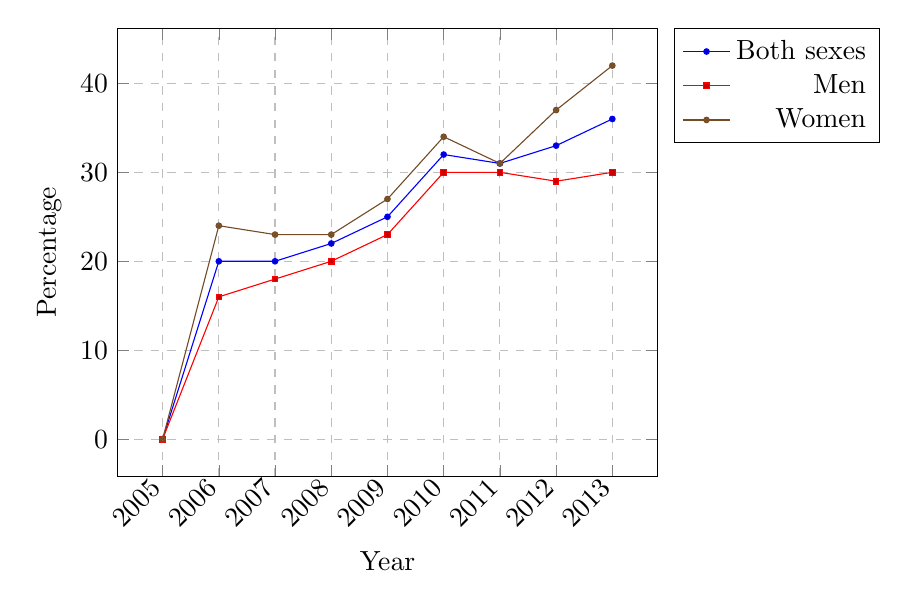
\begin{tikzpicture}
      \begin{axis}[
        xlabel={Year},
        ylabel={Percentage},
        legend style={cells={anchor=east}, legend pos=outer north east,},
        xtick=data,
        x tick label style={rotate=45, anchor=east, /pgf/number format/1000 sep=},
        mark size=1.0pt,
        grid=major,
        grid style={dashed},
      ]
      \legend{Both sexes, Men, Women}
      \addplot coordinates {
        (2005, 0)
        (2006, 20)
        (2007, 20)
        (2008, 22)
        (2009, 25)
        (2010, 32)
        (2011, 31)
        (2012, 33)
        (2013, 36)
      };
      \addplot coordinates {
        (2005, 0)
        (2006, 16)
        (2007, 18)
        (2008, 20)
        (2009, 23)
        (2010, 30)
        (2011, 30)
        (2012, 29)
        (2013, 30)
      };
      \addplot coordinates {
        (2005, 0)
        (2006, 24)
        (2007, 23)
        (2008, 23)
        (2009, 27)
        (2010, 34)
        (2011, 31)
        (2012, 37)
        (2013, 42)
      };
      \end{axis}
    \end{tikzpicture}
    \label{fig:ecommerce-in-norway}
    \caption{E-commerce purchases in Norway since 2005~\cite{statisticsNorway}}
  \end{figure}
}

\section{Motivation}
\label{sec:motivation}

% What are recommender systems good for?
In today's day and age the increasing amount of data overwhelm our human
processing capabilities in many information seeking tasks. To cope with this
overload researchers have introduced recommender system to filter the ever
increasing information and only present a small selection of items which
reflects the users tastes, interests and priorities. Recommender systems are an
active research field and has been successfully applied to many different
services ranging from e-commerce sites such as \emph{Amazon}, movie and
TV-series streaming services like \emph{Netflix} and in different music
applications such as \emph{Last.fm} and \emph{iTunes}.

% What is telenors incentive?
Many of the largest commerce Web sites have been using recommender systems to
help their customers find products to purchase for nearly two decades.
Schafer et al.~\cite{Schafer1999} identified three ways, in which recommender
systems increase E-commerce sales: (1) Browser into buyers: Recommender systems
can help customers find products they wish to purchase, (2) Cross-sell:
Recommender systems improve cross-sell by suggesting additional products for
the customer to purchase and (3) Loyalty: In a world where the competitor only
is one click away, gaining customer loyalty is an essential customer strategy.
Recommender systems improve loyalty by creating a value added relationship
between the site and the customer.

% What is the app and what makes it unique?
SoBazaar is a new \textit{fashion e-commerce application} for web and hand held
devices developed by Telenor, Norway's largest Telco company. The application
aggregates fashion products from various brands and stores into one \emph{news
feed} with recommended products, enabling the user to shop clothes and
accessories effortlessly and without the need of registering an account on
multiple web stores. Currently the application makes global recommendations
based on popular products and trends within social networks --- however, the goal
before launching the application this upcoming summer (\the\year) is to improve
these ratings making them personalized and grounded in a larger array of
features. This has as noted the potential of improving sales, activity and user
satisfaction.

% Discuss potential in fashion and e-commerce sales.
\ecommercenorway{}

The growth potential of such an application is immense in Norway. Numbers from
Statistics Norway~\cite{statisticsNorway} which are presented in the above
figure, shows a steady increase in the number of e-commerce sales of about 8\%
per year, from 2005. Still the competition, especially within personalized
recommendations, is insubstatial at both a national and international level, as
we will see in a detailed comptetitor analysis in
Section~\ref{subsec:competitors}. This underlines the importance of both the
discoveries made in this thesis and the application itself.

% Limited amount of data -> we need to utilize other sources. Implicit!
As the application is not yet officially released there is a limited amount of
user-item interaction from a set of beta users. In addition users do not have
the possibility to explicitly rate items on a numeric scale, a scheme often
employed by machine learning engineers and application developers in order to
understand their users preferences. Combining these two factors makes the
recommendation scenario both interesting and unique, since we need to utilize
the implicit information contained in user behavior such as clicking, wanting
or buying an item. Limited data both in number of users, but also in activity,
makes the system prone to what is called \textit{cold-start issues}, where
making recommendations with limited information is resolved by a variety of
techniques.

% The fashion domain have certain challenges.
This scenario differs from making recommendations on movies, books and music,
not just in the lack of rich explicit ratings, but also in the context of the
domain the recommendations will be done, namely the fashion domain. Firstly,
fashion consumption is largely determined by seasons. E.g. one does not buy
winter jackets in the middle of summer. Most clothes do also go out of
fashion, the same can not be said for \emph{all} movies. Secondly, there are a
whole different set of important aspects regarding the items or products when
recommending in the fashion domain, such as: brand, color and size.

% Brand and price are important!
Finally, users are highly price and brand-aware. This can be exemplified by
looking at an average movie consumer, where typically the director of the movie
does not greatly affect the way the movie is consumed. However, in the fashion
domain the consumer might mainly look at the product brand when deciding what
to consume. Price preferences are also related to this property where some
users prefer making \textit{a good deal} on periodic sales whilst other buys
clothes not only for individual satisfaction, but to show of or make a
statement.

% What are our goals and purpose?
In our system, there are two sources of information available for making
recommendations: an aggregated product database and event logs capturing user
activities. Out first goal is to find a technique for translating the implicit
feedback into preferences. These preferences are then combined with product
features and techniques for mitigating the cold-start problem. Finally the
user-item preferences are utilized in making recommendations where challenges
related to both domain and data sources are considered.

% Example scenario
For the users of SoBazaar the final product should not infer with the already
established user interface. Instead the news feed will evolve from today
showing the same recommendations to all users, to showing \textit{personalized
recommendations} to every user, based on their \textit{behavior} in the
application. For every user-item interaction the user is implicitly changing
his/hers preference-profile and will then, by just using the application, get
novel and more robust recommendations. Further, as personalized recommendations
hopefully will increase both sales and user activity we will, with a larger set
of data, be able to understand more user patterns and consequently gain a
deeper understanding of the domain.

\section{Problem Statement and Goals}

% Overall problem statement
The primary aim of this thesis is proposing a system, producing personalized
fashion recommendations based on user behaviour and product features, when both
resources are extremely limited in both quality and volume.

% Introduce goals related to domain
In order to propose such a system, one need a exhaustive understanding of both
the fashion domain and available data. In addition a study is required looking
at existing solutions, competitors and idientify potential competitive
advantages. Finally a discussion on how to overcome found challenges with
respect to both understanding the implicit feedback and making recommendations
is needed. Hence, our domain specific goals can be defined as:

% Domain-specific goals
\begin{itemize}
	\item \textbf{G1}: Gain a better understanding of the fashion domain.
  \item \textbf{G2}: Identify the specific challenges of making fashion recommendations.
  \item \textbf{G3}: Study how existing technologies can be adapted to mitigate or
  overcome these challenges.
\end{itemize}

% Introduce goals related to cold-start
In most recommender systems one base future recommendations on existing
feedback already given by the user. An important however is what to recommend
when no feedback has been given, which is the case for any new user. The same
issue is apparent when a new item is added to the application, where we need a
strategy for introducing it to users although the product is not connected to
any existing feedback. Finally, the closely related problem of making
recommendations in scenarios where feedback is extremely sparse need to be
addressed. First impressions are important both for retention and customer
satisfaction and consequently, seperate goals were set specifically concerning
cold-start issues.

\begin{itemize}
  \item \textbf{G4}: Study existing solutions to the cold-start.
  \item \textbf{G5}: Identify the best suited methods with regards to both application
  feedback and domain.
\end{itemize}

% Introduce goals related to implicit feedback
There is no explicit way for users to \textit{rate} or give \textit{negative
feedback} to items in SoBazaar. This forces us to look at user behaviour and
more specifically interactions on items such as \textit{clicking},
\textit{wanting} or \textit{purchasing}. We would like to learn how these
events could be used to predict the users true preferences. Using implicit
feedback yields the following goals:

\begin{itemize}
  \item \textbf{G6}: Explore the existing solutions of how to infer user preference from
  implicit feedback data.
  \item \textbf{G7}: Identify different methods of combining various event types into
  \emph{implicit ratings}.
  \item \textbf{G8}: Find metrics in order to evaluate the \emph{implicit ratings}.
\end{itemize}

% Introduce limitations
\paragraph{Limitiations} Our problem statement and consequent goals establish
the main theme of this thesis, but simultaneously they introduce some
limitiations. Hence, the reader should be familiar with what this thesis
\textit{does not set out to do}.

% Small and sparse dataset
The main limitiation of this thesis are primarly linked to having only one
available dataset with both sparse and modest data. As a result, making
conclusions based user behaviour proved difficult due to lack of statistical
significance on many observations. Limitiations in both time available and
number of existing users with sufficient activity made is also impossible to
conduct a thorough user study, which could confirm possible found user
patterns.

% No external sources of information (or weak quality)
In addition, as seen in the overview, external sources of information such as
social networks and trust-based networks are not considered --- as the dataset
provided did not warrant this. As the products in the SoBazaar application are
aggregated from multiple sources, and hence product databases, the quality of
information are notably diverse. Consequently, since extracting basic content
features different from product titles became close to impossible without large
engineering efforts, the \textit{main focus} does not lie on hybrid recommender
systems (combining content and user-based recommendations), although some work
is done in this area.

\section{Application Overview}

\begin{figure}[H]
  \centering
  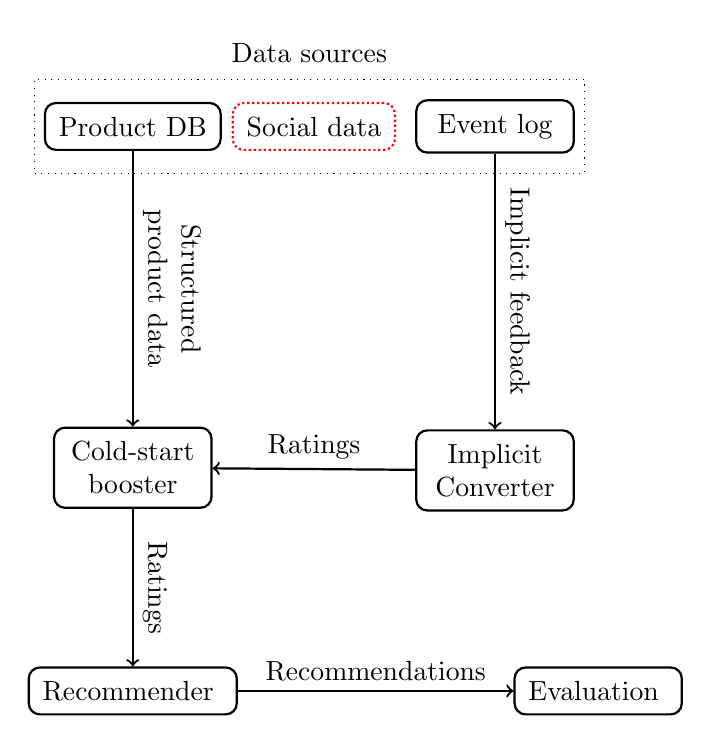
\begin{tikzpicture}[
    % Manually overriden in most of the nodes :-)
    node distance=2.3cm,
    block/.style={
      rectangle,
      draw,
      thick,
      inner sep=5pt,
      align=center,
      rounded corners,
      minimum width=2cm,
    },
    % Special style for the social networks
    social/.style={
      draw=red,
      densely dotted,
    },
    % Box surrounding the data sources.
    dsbox/.style={
      draw,
      dotted,
      minimum height=1.2cm,
    }
  ]

  % Create nodes - first, data sources.
  \node(db)     [block] {Product DB};
  \node(social) [block,social, right of=db] {Social data};
  \node(log)    [block,right of=social] {Event log};

  % Our various 'systems'
  \node(coldstart) [block, below = 3.5cm of db] { Cold-start\\booster };
  \node(converter) [block, below = 3.5cm of log] { Implicit\\Converter };
  \node(recommender) [block, below = 2cm of coldstart] { Recommender };
  \node(evaluation) [block, right = 3.5cm of recommender] { Evaluation };

  % Box around data sources.
  \node (datasources) [dsbox, fit=(db) (social) (log)] {};
  \node at (datasources.north) [above, inner sep=2mm] {Data sources};

  % Draw the links between systems and data sources.
  \path[->,thick]
     (log) edge [] node [sloped, above] {Implicit feedback} (converter)
     (db) edge [] node [sloped, above, text width=3cm, align=center] {Structured\\product data} (coldstart)
     (converter) edge [] node [sloped, above] {Ratings} (coldstart)
     (coldstart) edge [] node [sloped, above] {Ratings} (recommender)
     (recommender) edge [] node [sloped, above] {Recommendations} (evaluation);

  \end{tikzpicture}
  \caption{Application overview, showing input and output from different
  components in the proposed system}
\end{figure}

\section{System Overview}

\marginpar{Include filterbots in a more detailed system overview?}

This thesis proposes a system for making recommendations based on implicit
data, where the input is implicit feedback collected on a set of users and
items and the output is personalized recommendations to all users, proposing
new and relevant products to their preferences.

\begin{figure}[H]
  \centering
  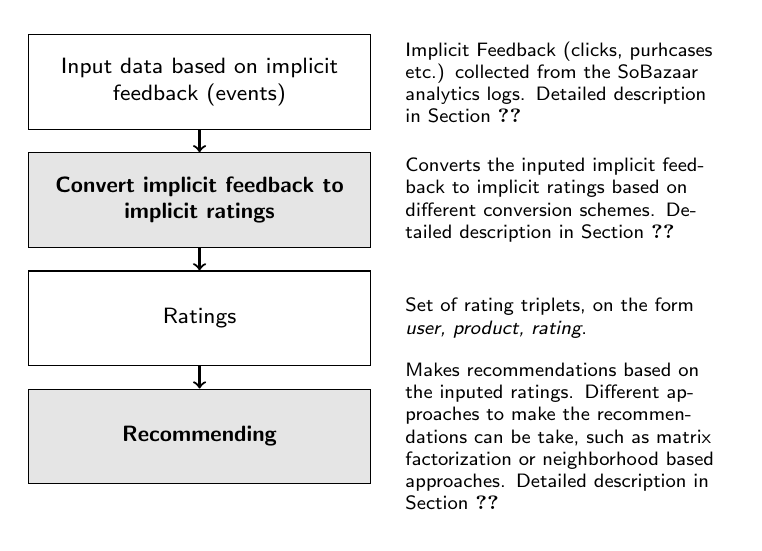
\begin{tikzpicture}
    [node distance = 1cm, auto,font=\footnotesize,
    % STYLES
    every node/.style={node distance=1.5cm},
    % The comment style is used to describe the characteristics of each process
    comment/.style={rectangle, inner sep= 5pt, text width=4cm, node distance=0.25cm, font=\scriptsize\sffamily},
    % The nonProcess style
    nonProcess/.style={rectangle, draw, inner sep=5pt, text width=4cm, text badly centered, minimum height=1.2cm, font=\footnotesize\sffamily},
    % The process style is used to draw the processs' name
    process/.style={rectangle, draw, fill=black!10, inner sep=5pt, text width=4cm, text badly centered, minimum height=1.2cm, font=\bfseries\footnotesize\sffamily}]

    % Draw processs
    \node [nonProcess] (inputData) {Input data based on implicit feedback (events)};
    \node [process, below of=inputData] (implicitConverter) {Convert implicit feedback to implicit ratings};
    \node [nonProcess, below of=implicitConverter] (ratings) {Ratings};
    \node [process, below of=ratings] (recommendations) {Recommending};

    \node [comment, right=0.25 of inputData] (comment-inputData) {
      Implicit Feedback (clicks, purhcases etc.) collected from the SoBazaar
      analytics logs. Detailed description in Section~\ref{sec:sobazaar-data}
    };

    \node [comment, right=0.25 of implicitConverter] (comment-implicitConverter) {
      Converts the inputed implicit feedback to implicit ratings based on
      different conversion schemes. Detailed description in
      Section~\ref{sec:implementation-implicit}
    };

    \node [comment, right=0.25 of ratings] (comment-ratings) {
      Set of rating triplets, on the form \textit{user, product, rating}.
    };

    \node [comment, right=0.25 of recommendations] (comment-recommendations) {
      Makes recommendations based on the inputed ratings. Different
      approaches to make the recommendations can be take, such as matrix
      factorization or neighborhood based approaches. Detailed description in
      Section~\ref{sec:making-recommendations}
    };

    % Draw the links between processs
    \path[->,thick]
      (inputData) edge (implicitConverter)
      (implicitConverter) edge (ratings)
      (ratings) edge (recommendations);

  \end{tikzpicture}
  \caption{Overview of the system. Boxes in white represents input and output
  data. Boxes in gray represents processes}
\end{figure}

Traditionally in most recommender systems this process does not include the
first two stages of our system, hence going directly from a set of explicitly
provided ratings to a set of recommendations. However, as we will see, making
ourselves non-dependent on explicit ratings can both provide us with a good
set of recommendations and take us one step closer to true artificial
intelligence, as we require no extra effort from the users --- rather learning
preferences from their behavior.

\section{Outline}
\begin{table}[H]
  \centering
  \begin{tabular}{lp{11cm}}
  \toprule
    \textbf{Chapter}      & \textbf{Description} \\
  \midrule

    Chapter \ref{chap:introduction} & The~\nameref{chap:introduction} chapter gives an overview of the
    project to the reader. It also outlines the purpose and motivation of the
    project.  \\[1.5ex]

    Chapter \ref{chap:thesobazaardata} & \nameref{chap:thesobazaardata} chapter presents the results from our
    dataset analysis. \\[1.5ex]

    Chapter \ref{chap:SotA} & The \nameref{chap:SotA} chapter documents knowledge,
    research and technology that are relevant to the project, and how and why
    some of them were prioritized over others when it comes to how they are
    used in the project. \\[1.5ex]

    Chapter \ref{chap:implementaion} & The \nameref{chap:implementaion} chapter describes the design of the
    system and how the design has been implemented. \\[1.5ex]

    Chapter \ref{chap:resulteval} & The \nameref{chap:resulteval} chapter discus the development process,
    testing of results and major issues. \\[1.5ex]

    Chapter \ref{chap:conclusion} & The \nameref{chap:conclusion} chapter sums up the project and describes the
    findings and reflects on them. It also describes further work.
    \\[1.5ex]

    Appendix & \textbf{The Appendix} contains extended information such as a full list of the requirements. \\

  \bottomrule
  \end{tabular}
  \caption{Overview of structure and chapters in the thesis}
  \label{table-reportstructure}
\end{table}

% !TEX root = ../report.tex

\chapter{The SoBazaar Data}
\label{chap:thesobazaardata}
\minitoc

This chapter will in greater detail explore the SoBazaar application and
explore the current state of the dataset used in this thesis. Further,
interesting discoveries are presented, which all has an impact on \textit{how}
we go forth and build a recommender engine for a fashion application. In order
to best understand the domain in question, and answer research goal \textbf{G1}
and \textbf{G2}, this chapter serves an important role for future chapters.
Many identified properties of the dataset explored in this chapter will give
reason to the majority of choices made throughout the thesis.

\clearpage


\begin{chapquote}[30pt]{About SoBazaar}
  "SOBAZAAR is a newly developed social shopping experience -- a daily fashion bazaar on your mobile."
\end{chapquote}

SoBazaar is an online marketplace for fashion, but with a social twist. You can
find stores like Moods of Norway, BIK BOK, Bianco and many more, which all have
their own \textit{storefront} in the application. The application lets you
browse through thousands of products, presenting them in a \textit{newsfeed},
which in todays state yields global recommendations to all users based on the
opinions of professional fashion experts. If you find something you like you
can purchase it directly from the application or store it for later with the
\emph{heart it} function, which in this thesis is refered by its backend name
\textit{product wanted}. The following screenshots highlights some
functionality currently found in the application. In the leftmost screenshot a
set of items are presented in the newsfeed, together with the name of a user
(not necessarily connected to the logged in user) who has liked these items.
The two remaining screenshots, also taken from the newsfeed, shows how brands
are able to notify users on sales and new products, in addition to showing the
most popular products at the moment.

\begin{figure}[H]
  \centering
  \begin{minipage}{.30\linewidth}
      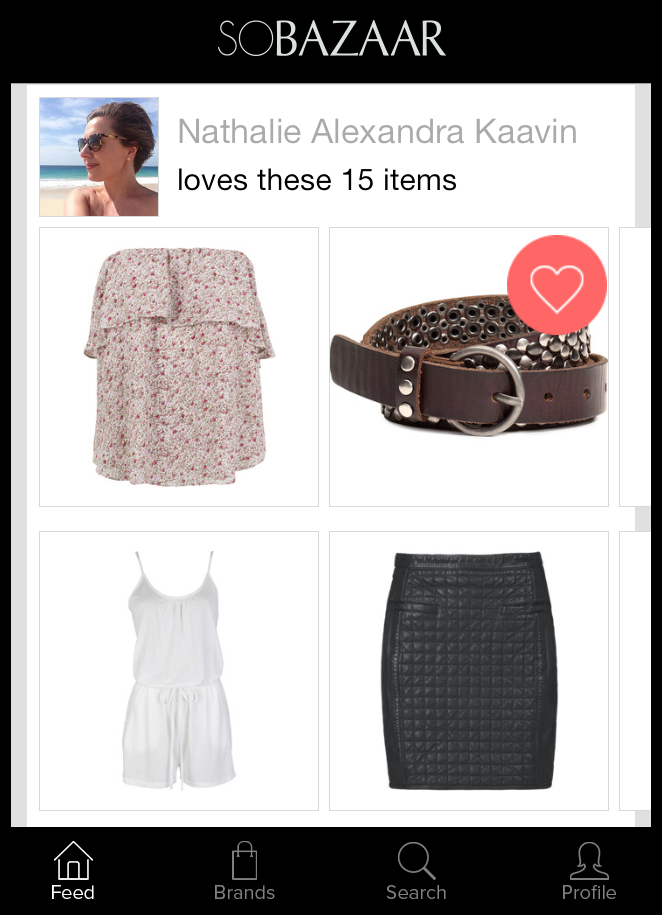
\includegraphics[height=1.5\linewidth]{image/SoBazaarfeed.png}
  \end{minipage}
  \hspace{.02\linewidth}
  \begin{minipage}{.3\linewidth}
        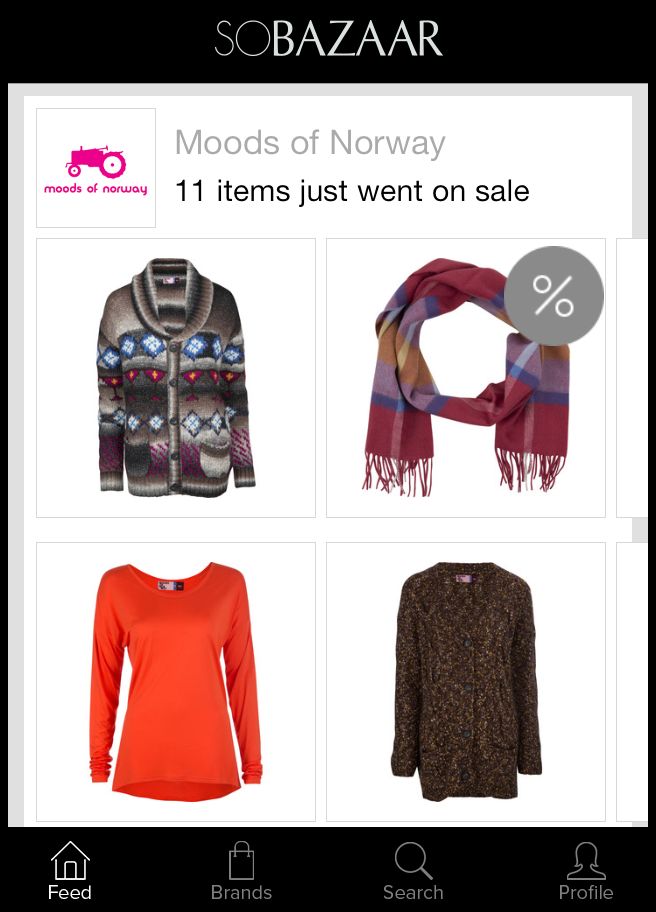
\includegraphics[height=1.5\linewidth]{image/SoBazaarsale.png}
  \end{minipage}
  \hspace{.02\linewidth}
  \begin{minipage}{.30\linewidth}
      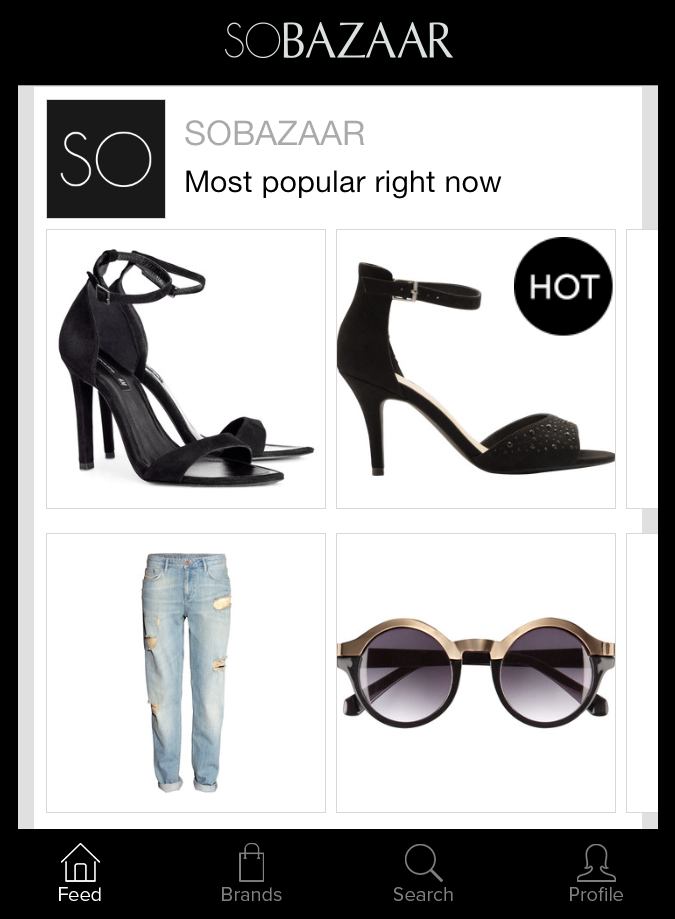
\includegraphics[height=1.5\linewidth]{image/SoBazaarmostpop.png}
  \end{minipage}
  \caption[SoBazaar newsfeed screenshots - version 0.5.1]{Screenshots from the
  SoBazaar newsfeed.}
  \label{figure:SoBazaarfeed}
\end{figure}

Users are also able to browse \textit{by brand} or storefront, as shown in the
leftmost screenshot below. A storefront is different from a brand-store by
combining products from a variety of brands into categorical sales or
\textit{packages} such as \textit{«summer sale»}. One of these storefronts are
coined \textit{Editor's picks}, which as we have mentioned, are curated by
professionals. If a brand or storefront is clicked one is taken to a custom
listing, presenting all products available together with their price and
optional status such as \textit{Hot} or \textit{New}.

\begin{figure}[H]
  \centering
  \begin{minipage}{.30\linewidth}
  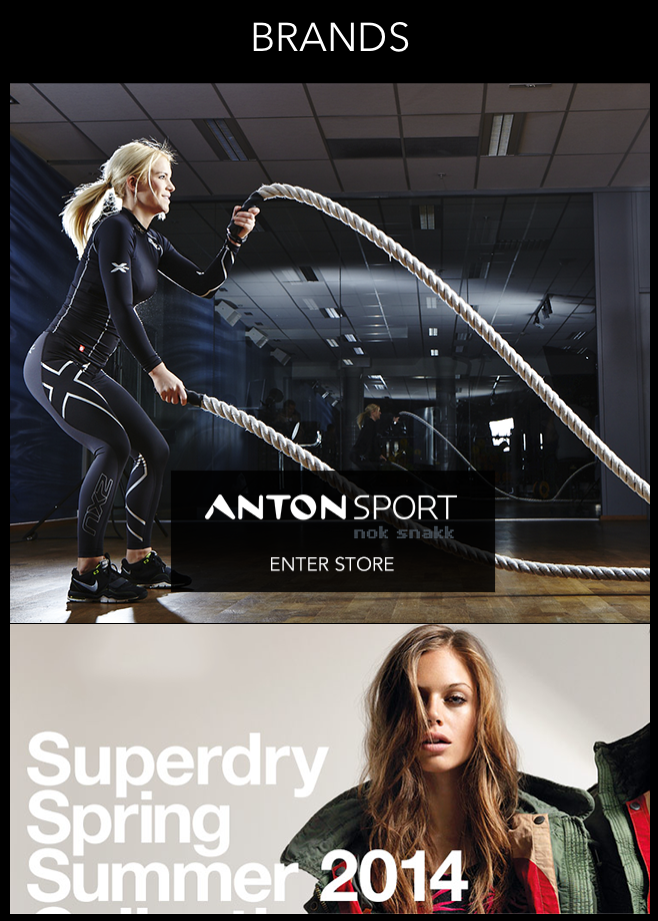
\includegraphics[height=1.5\linewidth]{image/SoBazaarbrands2.png}
  \end{minipage}
  \hspace{.02\linewidth}
  \begin{minipage}{.3\linewidth}
    
\includegraphics[height=1.5\linewidth]{image/SoBazaareditor.png}
  \end{minipage}
  \hspace{.02\linewidth}
  \begin{minipage}{.3\linewidth}
      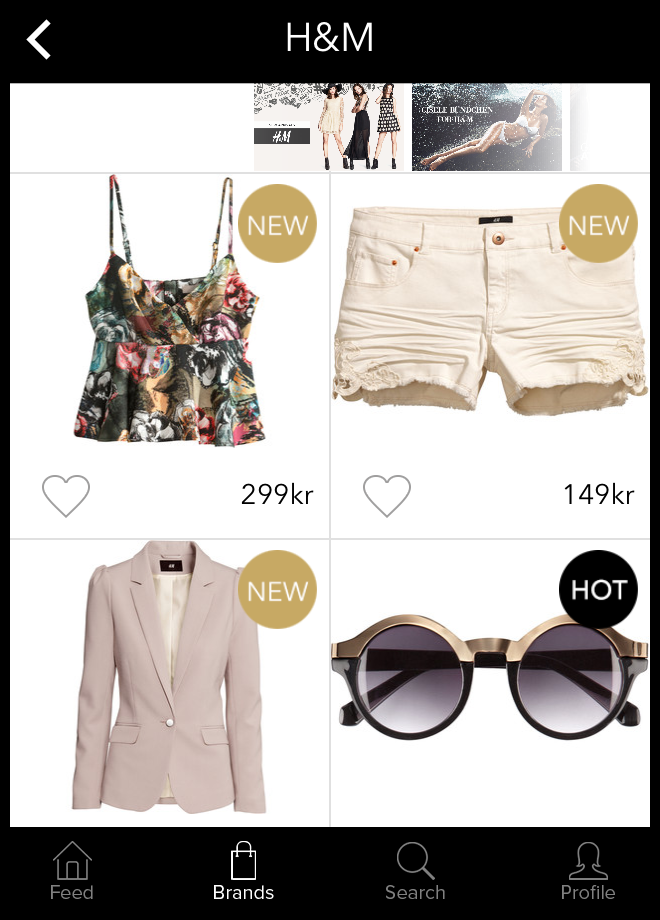
\includegraphics[height=1.5\linewidth]{image/SoBazaarStore.png}
  \end{minipage}
  \caption[SoBazaar storefront screenshots - version 0.5.1]{Screenshots from the SoBazaar Application. From the left to right: the brand browser, editors picks and the H\&M storefront}
  \label{figure:SoBazaarfeed}
\end{figure}

From the product screen you can choose to buy the item, being redirected to an
external online shop for completing the purchase. The product screen currently
features a \emph{«People who like this also love»} section, in addition to show
other products from the same store. Clicking the map marker a map showing
nearby physical stores selling the item is expanded. Furthermore, the
info-button yields a more detailed description of the product and pressing the
rightmost arrow one has the possibility of sharing the item with friends via.
various social networks. The application also features a personal page for
earlier saved or \emph{wanted} items, named \textit{My love list}. Finally, the
application supports simple search queries on product descriptions, titles and
brand names. As can be seen from the rightmost image it is also possible to
filter the results by status, brand and category (type of attire).

\begin{figure}[H]
    \centering
    \begin{minipage}{.30\linewidth}
          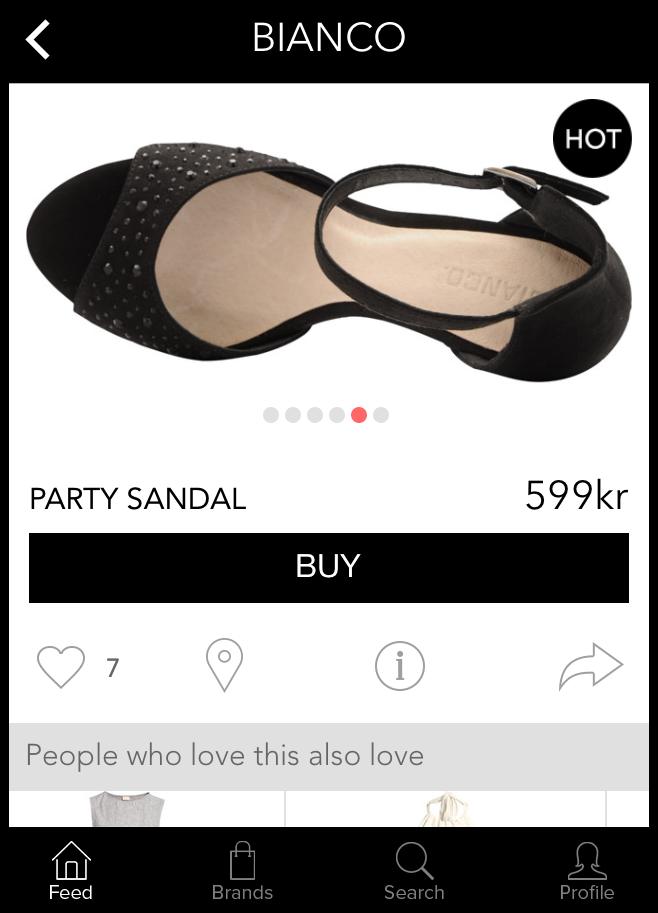
\includegraphics[height=1.5\linewidth]{image/SoBazaarproduct.png}
    \end{minipage}
    \hspace{.02\linewidth}
    \begin{minipage}{.3\linewidth}
      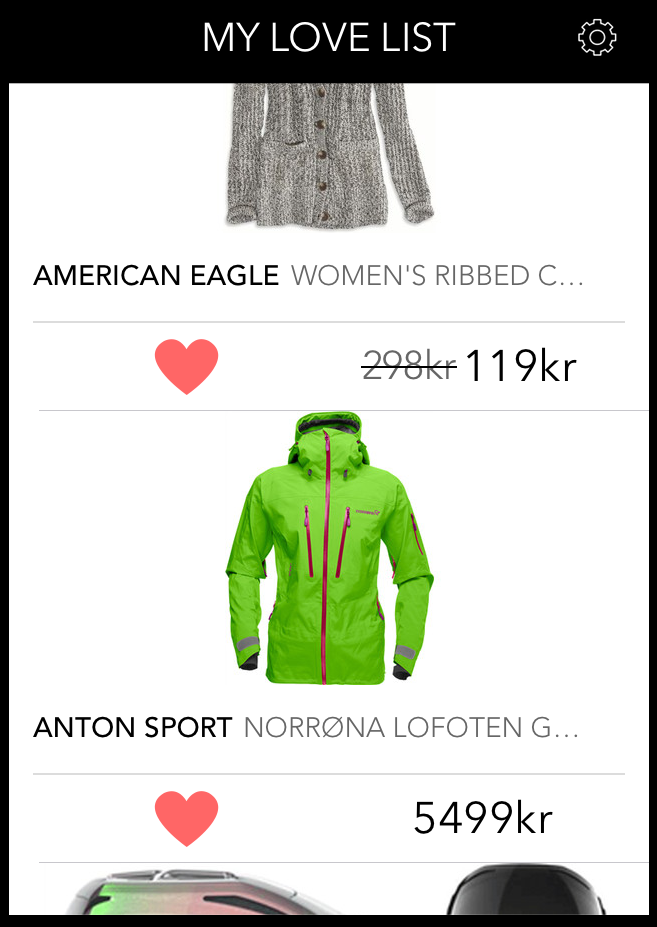
\includegraphics[height=1.5\linewidth]{image/SoBazaarlovelist.png}
    \end{minipage}
    \hspace{.02\linewidth}
    \begin{minipage}{.3\linewidth}
        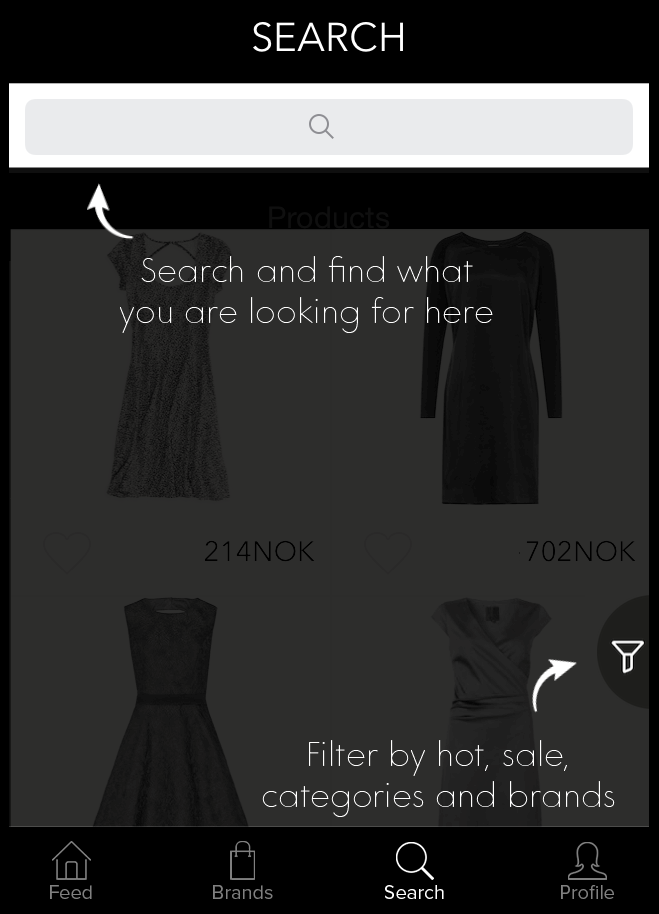
\includegraphics[height=1.5\linewidth]{image/SoBazaarsearch.png}
    \end{minipage}
    \caption{Screenshots showing product details, love list and search
    functionality}
    \label{figure:SoBazaarfeed}
\end{figure}

The application is currently in a beta phase and is planned for a final release after the summer.

\section{Preprocessing}
\label{sec:preprocessing}

In data mining, preprocessing is an important procedure which lays the
foundation for further data analyzation. The saying \emph{garbage in, garbage
out}~\cite{GIGO} especially applies here, as the quality of input data can make or
break the final results. This is due to a variety of reasons, ranging from
non-complete raw-values, events outside target groups or outliers having
user-beahviours which makes learning stereotypical patterns impossible.

The following pre-processing steps were performed before continuing to analyze
the dataset:

\begin{itemize}
  \item Anonymization of all personal information, including positional data.
  \item Removal of all events made in test or staging environments.
  \item Removal of suspicious users having activity levels multiples above
  normal. The majority of these events were made in the early phase of the
  application.
\end{itemize}

As part of the preprocessing, a unique \textit{session identfier} field was
added to the data, indicating which events were done in the same timespan
without closing the application. This, as we will see in later sections helps
us understand multiple usage patterns.

\section{Dataset Overview}

The data from SoBazaar is based on all actions, also called events, made by the
users. They can range from accessing a storefront, scrolling the page or
purchasing a product. Combined, they form the basis of which we develop all
techniques in this thesis. When an event is triggered a set of information is
stored regarding the event, describing the \textit{context} of which the event
was fired, where the most relevant event-metadata, in terms of recommender
systems, are presented in the table below.

\begin{table}[H]
    \centering
    \begin{tabular}{l p{11cm}}
        \toprule
        Variable     & Explanation   \\
        \midrule
        \emph{product\_id}        & Unique id of the item on which the event
                                    was triggered \\
        \emph{user\_id}           & Unique id of the user who triggered the event \\
        \emph{event\_id}          & What kind of event was
                                  triggered~\tablefootnote{Complete list of the
                                  different types of events can be found in
                                  table~\ref{table:events}} \\
        \emph{price}              & The price (in NOK) of the item \\
        \emph{retailer\_brand}    & Unique id of the item retailer. A retailer
                                    is a distributer of products, such as H\&M,
                                    Cubus or Moods Of Norway \\
        \emph{storefront\_id}     & The storefront id of the storefront entered.
                                    A \textit{retailer\_brand}s can have multiple
                                    \emph{store\_fronts}. \\
        \emph{event\_location}    & The location of the user when the event was triggered \\
        \emph{ts}                 & Unix timestamp in milliseconds of when the event was triggered \\
        \emph{session}            & Which session number the event belongs
                                  to~\tablefootnote{This is the value added in the preprocessing
                                  phase~\ref{sec:preprocessing}. For two events to end up in the same
                                  session, the event has to be triggered within a certain period of time,
                                  and both be after the same application started-flag} \\
      \bottomrule
    \end{tabular}
    \caption[Event Metadata]{Metadata collected from an event. The complete list can be found in table~\ref{table:completeEventData}}
    \label{table:eventData}
\end{table}

These events are used to derive information regarding both users and products
-- and combined and structured they form what we call \textit{implicit
feedback}. After preprocessing the data we look at some key figures, in order
to better understand its properties.

    \begin{table}[H]
        \centering
        \begin{tabular}{l l}
            \toprule
            Attribute       & Count   \\
            \midrule
            Total number of product events &    40773 \\
            Unique users ids    &    2021 \\
            Unique item ids     &    6092 \\
            Unique storefronts  &    147~\tablefootnote{A storefront is a access point, with different clusterings of items. Stores can have multiple storefronts} \\
            Unique retailer brands  &    24 \\
            \hline
            Item clicks     &    25491 \\
            Item wants   &    13262 \\
            Item purchases   &    2020 \\
            \hline
            First event & Mon, 07 Oct 2013 10:59:57 GMT \\
            Last event & Mon, 19 May 2014 22:51:19 GMT \\
            Lifetime of data & 224 days \\
            \hline
            Average item click count per user   &    12.6130 \\
            Average item want count per user     &    6.5620 \\
            Average item purchase count per user     &    0.9995 \\
            \hline
            Average item interaction count per user     &    20.1746 \\
            Average user interaction count per item     &    6.6928 \\
            \bottomrule
        \caption[Dataset summary]{Overview of the key figures in the SoBazaar dataset}
        \label{table:datasetSummary}
        \end{tabular}
    \end{table}

    As seen from table~\ref{table:datasetSummary} the average amount of \emph{purchases} per user are below one. Using purchase information alone to make recommendations will therefore in most cases render the recommendations incomplete. If one or more users have more than one purchases, then some users will of course have none purchases. Making personalized recommendations for these users will then be unattainable.

    \emph{Clicks} and \emph{wants} on the other hand have a much higher occurrence. These two events together with \emph{purchases} tops a count of 20 on average per user, and opens for the possibility of more dense personalized recommendations, but the data is still rather sparse.

\section{Visualizations and analysis}
    % New graphs when/if:
    % Price range of items in stores
    % unique Stores count for users
    %     price span for user
    %         Timespann of sessions for users (avg, max, min)
    %         Events per session (avg, max, min)
    %         Item viewtime for user in session
    %         Stores visited per session
    %         revisit time of items for user
    %         relationship with view, want and purchase
    %         time of session over lifetime of app
    %         user preferred price in session
    %         price vs view, want and purchase
    %         avg viewtime for an item (i know)
    %         Similarity of user favorite store, items viewed and items wanted?
    %         time of session over lifetime of app for all users (slope-style)
    % check for price distribution based on location.
    % make price user graph
    % price for store dist
    This section will look at the SoBazaar data through visualizing the data and clearly communicating the information trough graphical means.
    It will start with the properties of the users seen in the data, then move over to the products and finally the time properties of the data.

\subsection{User properties}
    The properties of the users of the SoBazaar application can help understand how the application is used, and to get a better understanding of how to make predictions for them.

    The first figure visualizing the user behavior is a figure of the event distribution, and shows the events the users are triggering, and to what extend they do so.
    \begin{figure}[H]
        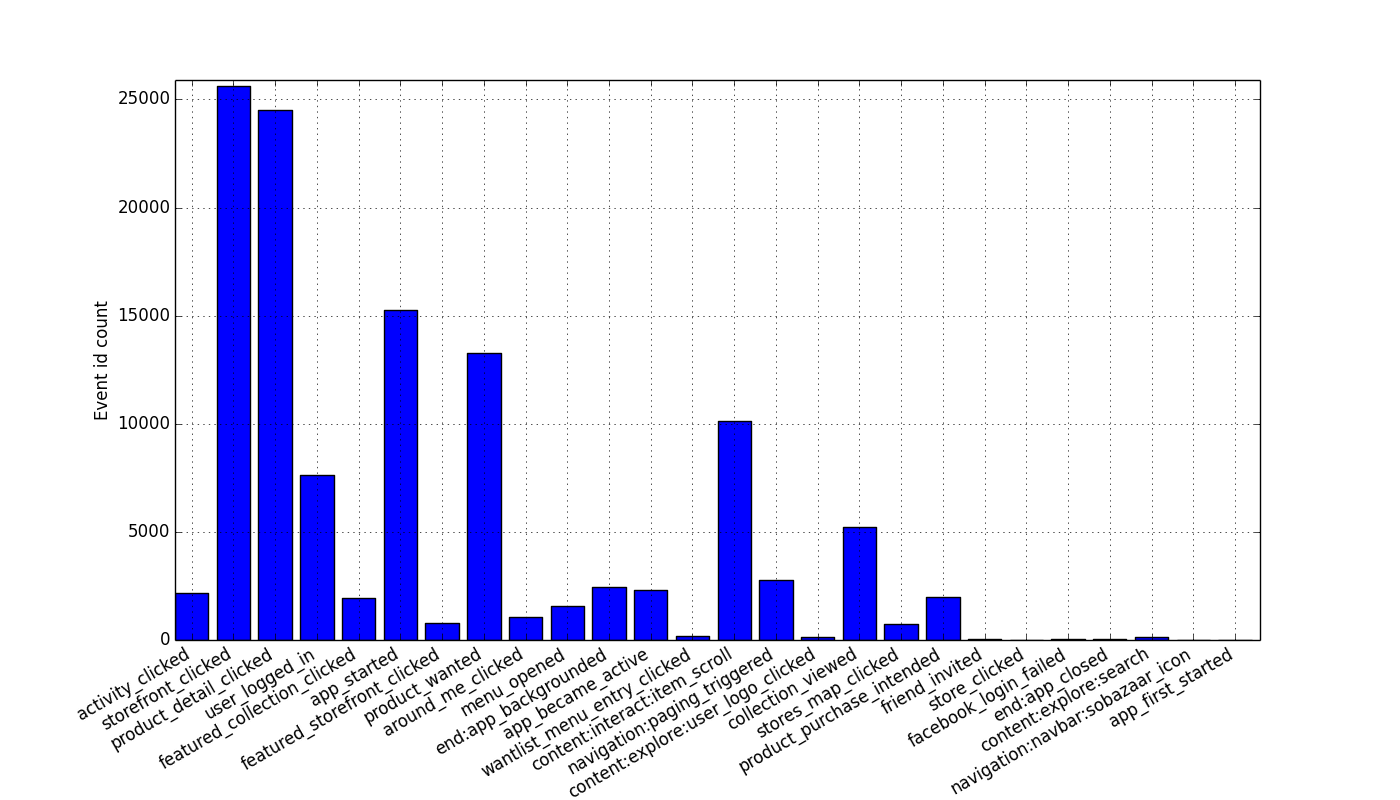
\includegraphics[width=5in]{image/event_iddistribution.png}
        \centering
        \caption{Event distribution}
    \label{figure:eventIDDistribution}
    \end{figure}
        In the figure above (figure~\ref{figure:eventIDDistribution}) we see the count for each of the different events which can be triggered in the SoBazaar application\footnote{With the exception of the event types with a trigger count lower than 200, which are merged into on bar and labeled \emph{other}}.
        As seen from the graph the \emph{product\_detail\_clicked}-event and the \emph{storefront\_clicked}-event are the two most common events to be triggered.
        As mentioned earlier in~\ref{table:eventData}, the \emph{storefront} is the main access point to a set of products, and the high values for this \emph{event\_id} is as expected.
        The fact that accessing the \emph{storefront} is the most occurring event, over clicking an item, indicates that many users browse the items through looking at the thumbnails rather than accessing the actual item.

        The \emph{product\_wanted}-event is the fourth most occurring event, and is about half the size of the \emph{product\_detail\_clicked}-event, this does not imply that half of the users accessing an item also adds the accessed item to their want list, since it is possible to want an item without accessing the item.
        \emph{product\_purchase\_intended} on the other hand has to come after a \emph{product\_detail\_clicked}, so it is therefore safe to assume that about 8\% of item accesses progressed into an intended purchase.

        Some of the evens shown above are newly added events, and the data has to mature more for more certain conclusion to be drawn.

        The distribution of events for the users are show in the next figure, and is intended to give a better overview of to what extent the users interact with the applications, and how the usage is distributed amongst the users.

    \begin{figure}[H]
        \centering
        \begin{subfigure}{.5\textwidth}
            \centering
            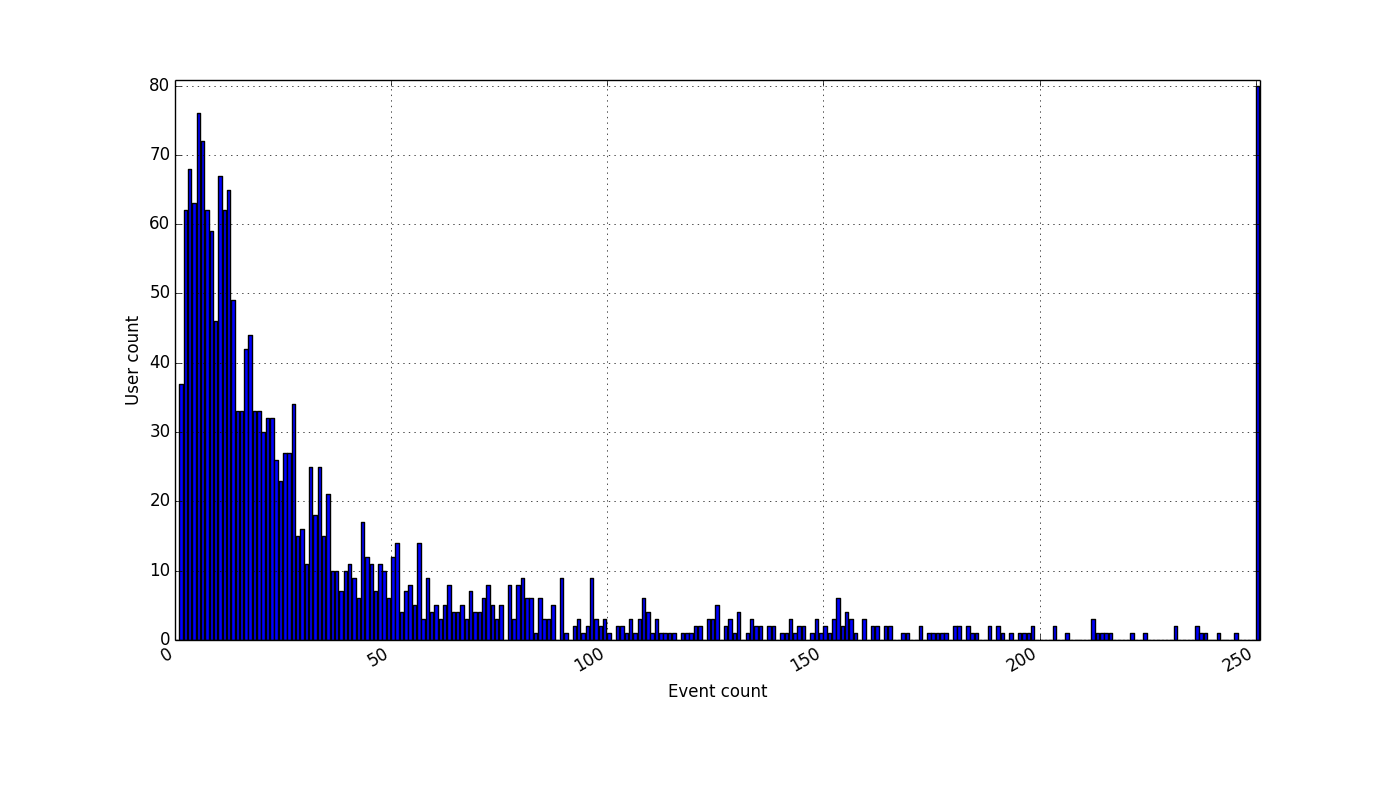
\includegraphics[width=\dualGraphWidth]{image/user_iddistribution.png}
            \caption{Distribution of events on users}
    \label{figure:userEventDist}
        \end{subfigure}%
        \begin{subfigure}{.5\textwidth}
            \centering
            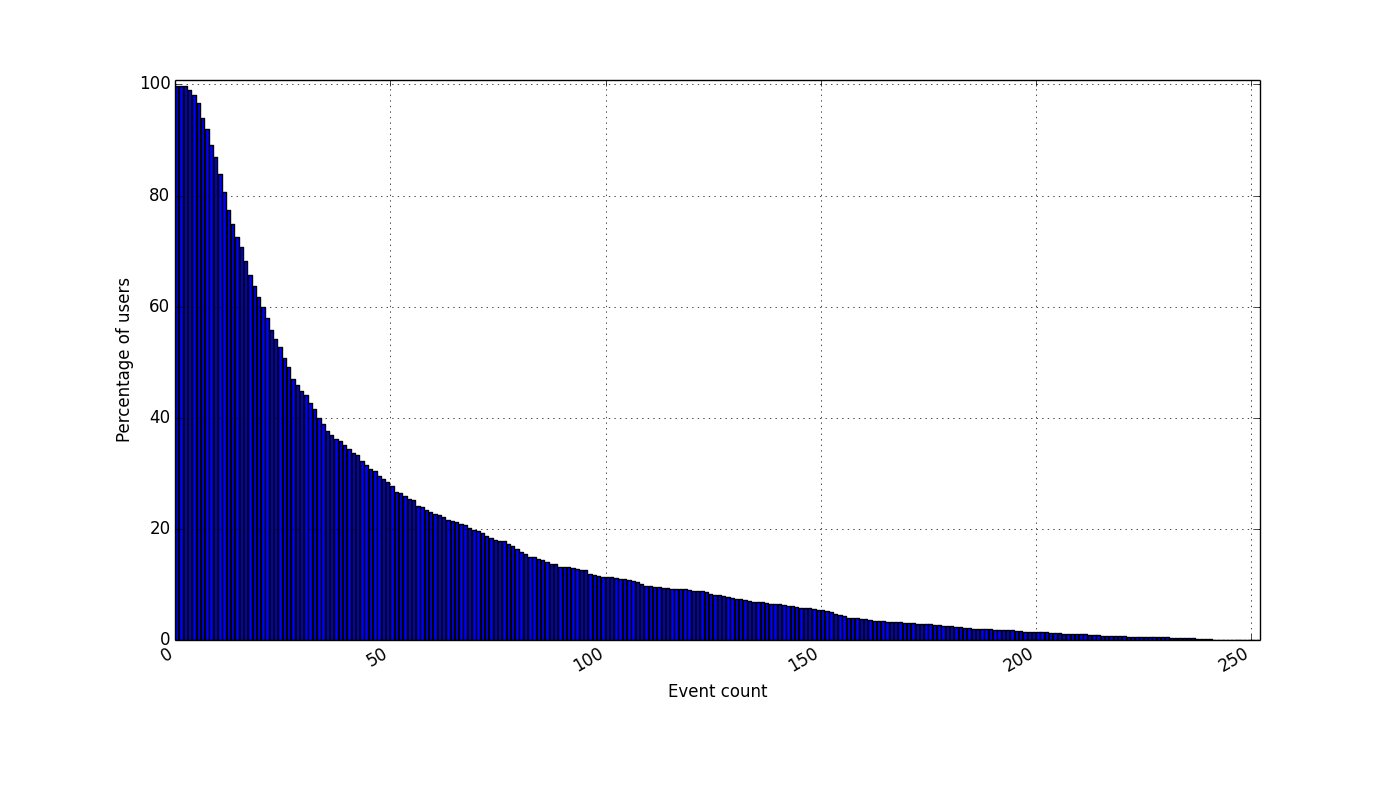
\includegraphics[width=\dualGraphWidth]{image/user_idcumdistribution.png}
            \caption{Cumulative distribution of events on users}
    \label{figure:userEventCumDist}
        \end{subfigure}
        \caption{Graphs presenting the distribution of events per user}
    \end{figure}
        Figure~\ref{figure:userEventDist} is showing the actual amount of users with the different counts of events.
        78\% of the users have 50 or less events, with the mean being at 5 events.
        The figures are showing the values from 0 to 250 since 96\% of the users resides in this subset of the data.

        As seen from figure~\ref{figure:eventIDDistribution} most of the events are not directly related to products, from table~\ref{table:datasetSummary} we can see that there are over 6000 products, and as mentioned above, 78\% of the users have less than 50 events. Based on these three facts, we can assume that the data is extremely sparse and measures to deal with this must be implemented.

        The distribution of events on the users tells us how the users interact with the applications, and how the events are distributed, but events are all actions taken by the users, and some of these might not be interesting when making recommendations for the users.
        A reduced view of the one seen in the figures above are shown in the figures below, where the only events considered are item interaction events.

    \begin{figure}[H]
        \centering
        \begin{subfigure}{.5\textwidth}
            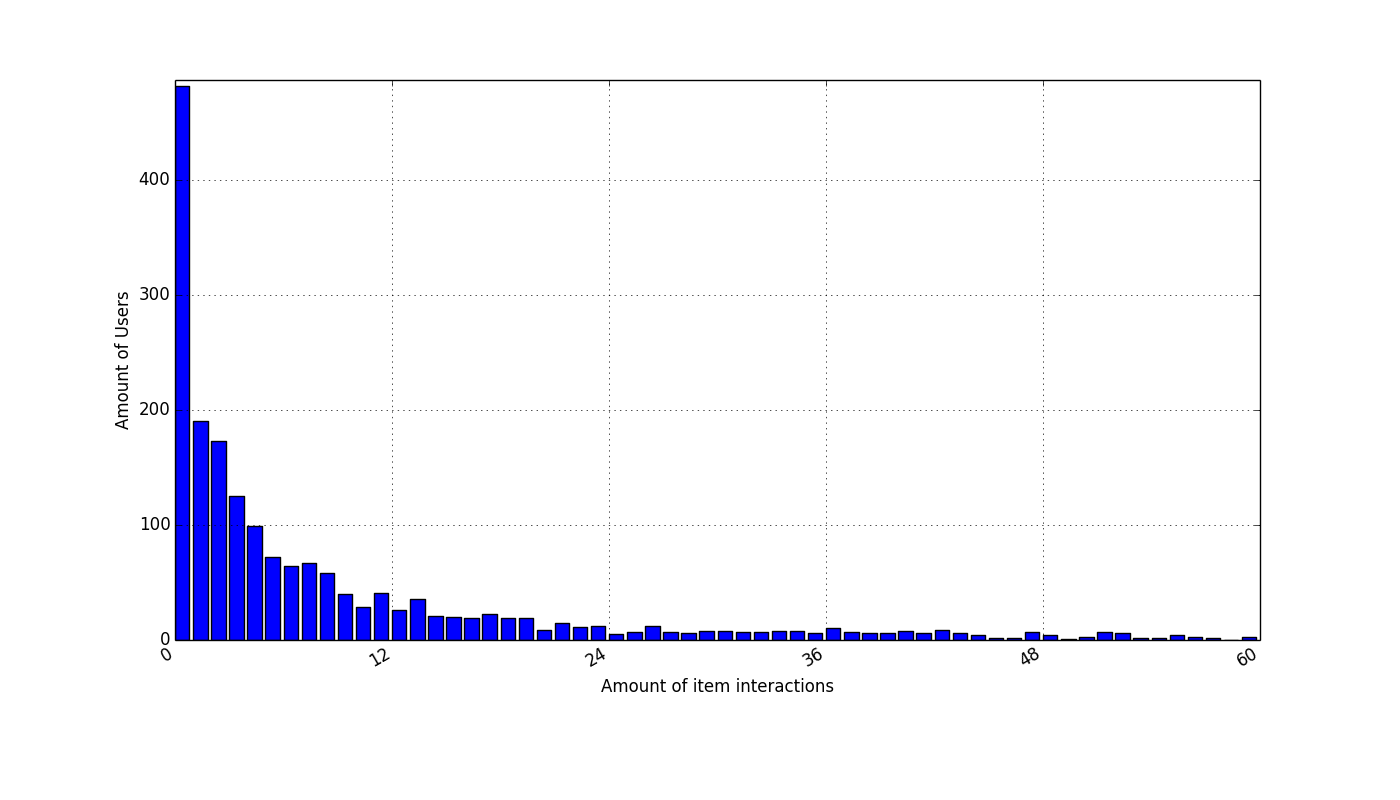
\includegraphics[width=\dualGraphWidth]{image/ratingsPerUserdistribution.png}
            \centering
            \caption{Count of item interactions for users}
    \label{figure:ratingsPerUser}
        \end{subfigure}%
        \begin{subfigure}{.5\textwidth}
            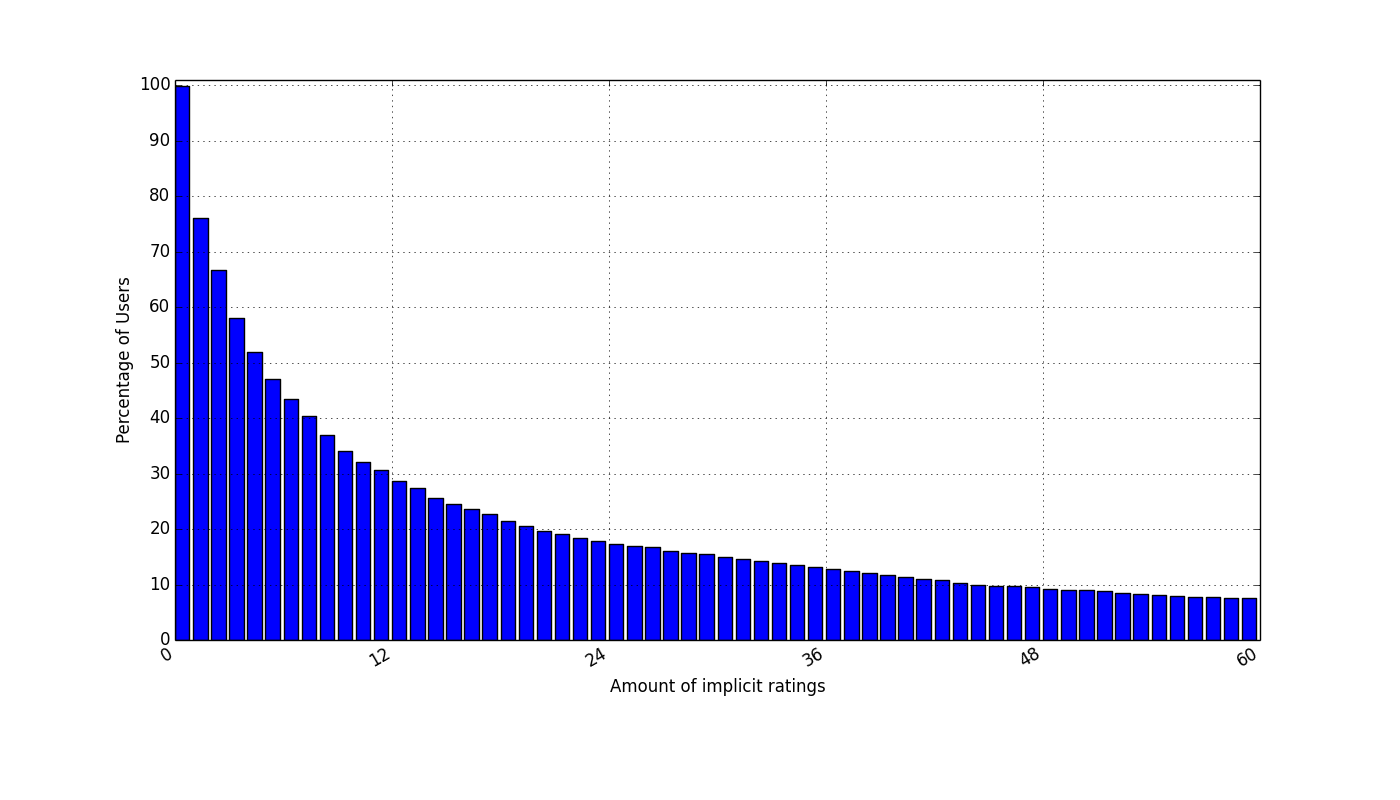
\includegraphics[width=\dualGraphWidth]{image/ratingsPerUsercumdistribution.png}
            \centering
            \caption{Cumulative count of item interactions for users}
    \label{figure:ratingsPerUserCum}
        \end{subfigure}
        \caption{Figures presenting the number of product interactions for the users in the data}
    \end{figure}
        In the figures above the rightmost bar present 0 product interactions.
        The graphs are limited to only showing interaction amounts up till 60 to give focus to the numbers where more than 90\% of the users resides.

        As seen from figure~\ref{figure:ratingsPerUserCum}, over 20\% of the users have never interacted with an item, and about 10\% of the users have more than 50 item interactions.

        Even though the data is sparse, as seen from the previous figures, the fact that the majority of the users have in some way interacted with at least one item, opens for the possibility of connecting users based on their item interactions.

        Now that we have looked at the distribution of events both as a whole, and as a reduced view, we might benefit from looking at how often the users use the application. The figure below shows the number of sessions for the users.

    \begin{figure}[H]
        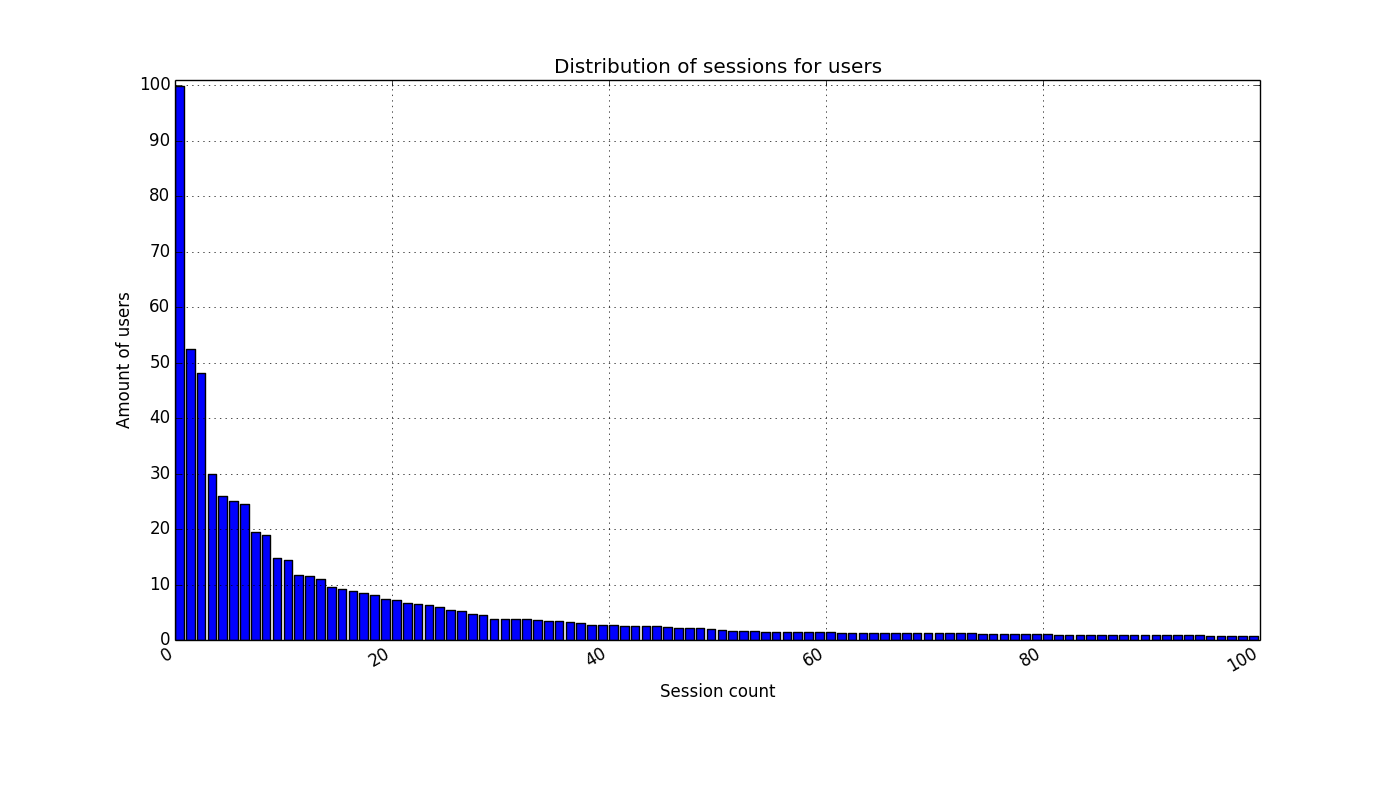
\includegraphics[width=5in]{image/sessiondistribution.png}
        \centering
        \caption{Distribution of sessions for users}
    \label{figure:sessCountDist}
    \end{figure}
        The figure above shows the count of sessions for the users of the SoBazaar application, with the users with more than 30 sessions removed.

        More than 90\% of the users of SoBazaar have a session count of 20 and less.
        This means that they have not logged on to the applications more than 20 separate times, over the time the data was collected, and strengthens the hypothesis that the data from SoBazaar is sparse.

        In figure~\ref{figure:sessCountDist} the 4 first bars sums up to 1000, which is the amount of users who has had 4 or less sessions on the application in total. In other words -- half of the users used the application less than 4 times.

        After having looked at the usage distribution of the users , we move over to the user account lifetime, to see actually how long a user is active on the application in terms of time from first to last recorded event for the user.

    \begin{figure}[H]
        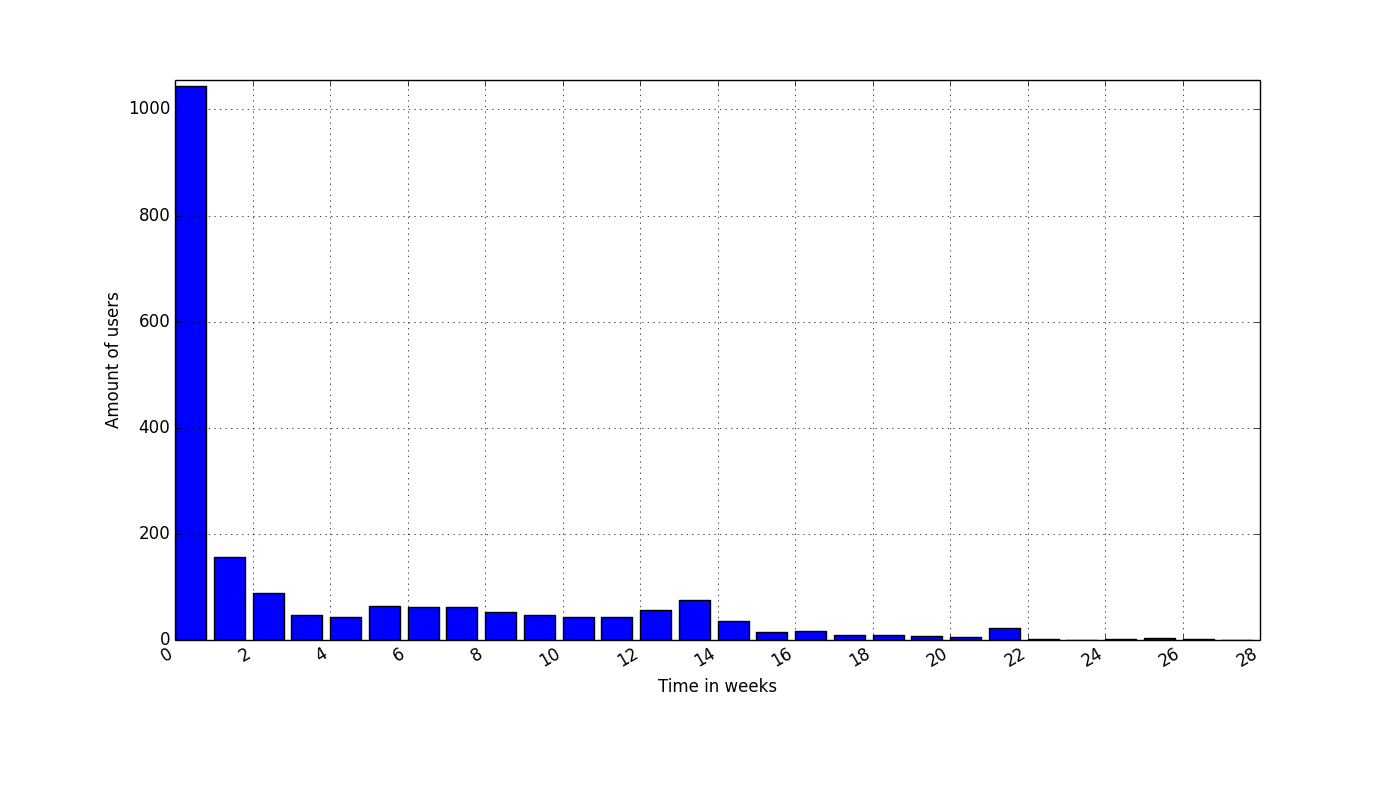
\includegraphics[width=5in]{image/userTimespansdistribution.png}
        \centering
        \caption{Distribution of user account lifetime}
    \label{figure:userTimespandist}
    \end{figure}
        The figure above displays the lifetime of the user accounts in the application in weeks, where the lifetime is measured from the first occurrence of the unique user id till the last event triggered by that user.

        From this figure it is apparent that over half of the user accounts have a lifespan of less than a week.

        Lifetime of the accounts mapped together with their usage might tell us more than just the account life time alone, so the next figure displays just that.

    \begin{figure}[H]
        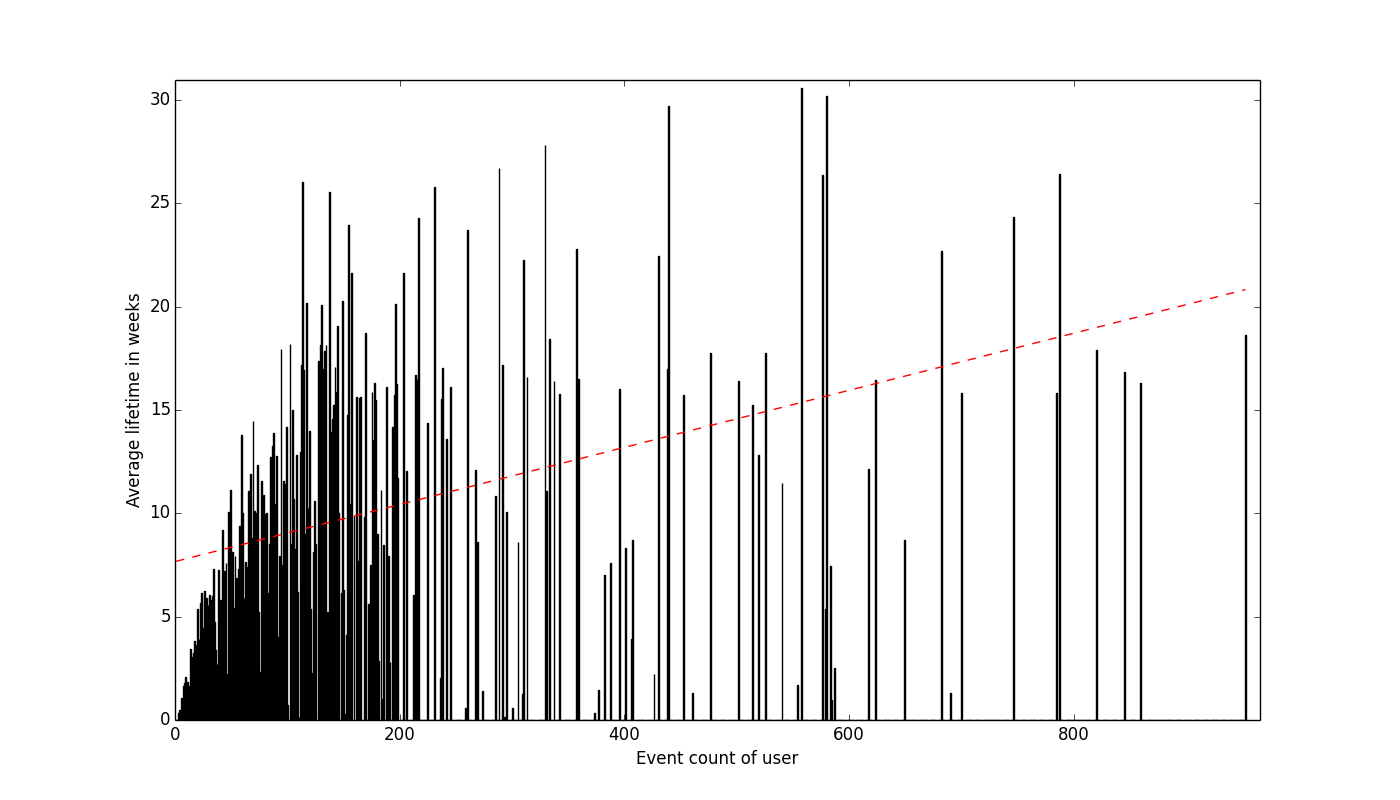
\includegraphics[width=5in]{image/avglifetimeoncountuser.png}
        \centering
        \caption{Average lifetime of user accounts sorted on event count}
    \label{figure:avglifetimeoncountuser}
    \end{figure}
        The figure above shows the lifetime of the user accounts together with their application interaction count.
        Users more to the right have a higher event count.
        Some outliers have been removed to give focus to the majority of the users. As mentioned earlier, 78\% of the users have triggered 50 or less events.

        The red line is the regression line of the user account lifetimes, and is there to show how the account life span increases with the amount of events.

        As seen in the data set overview table~\ref{table:eventData}, the location of the user at event trigger is stored in the data. The locations of the users are shown in the figure below.

    \begin{figure}[H]
        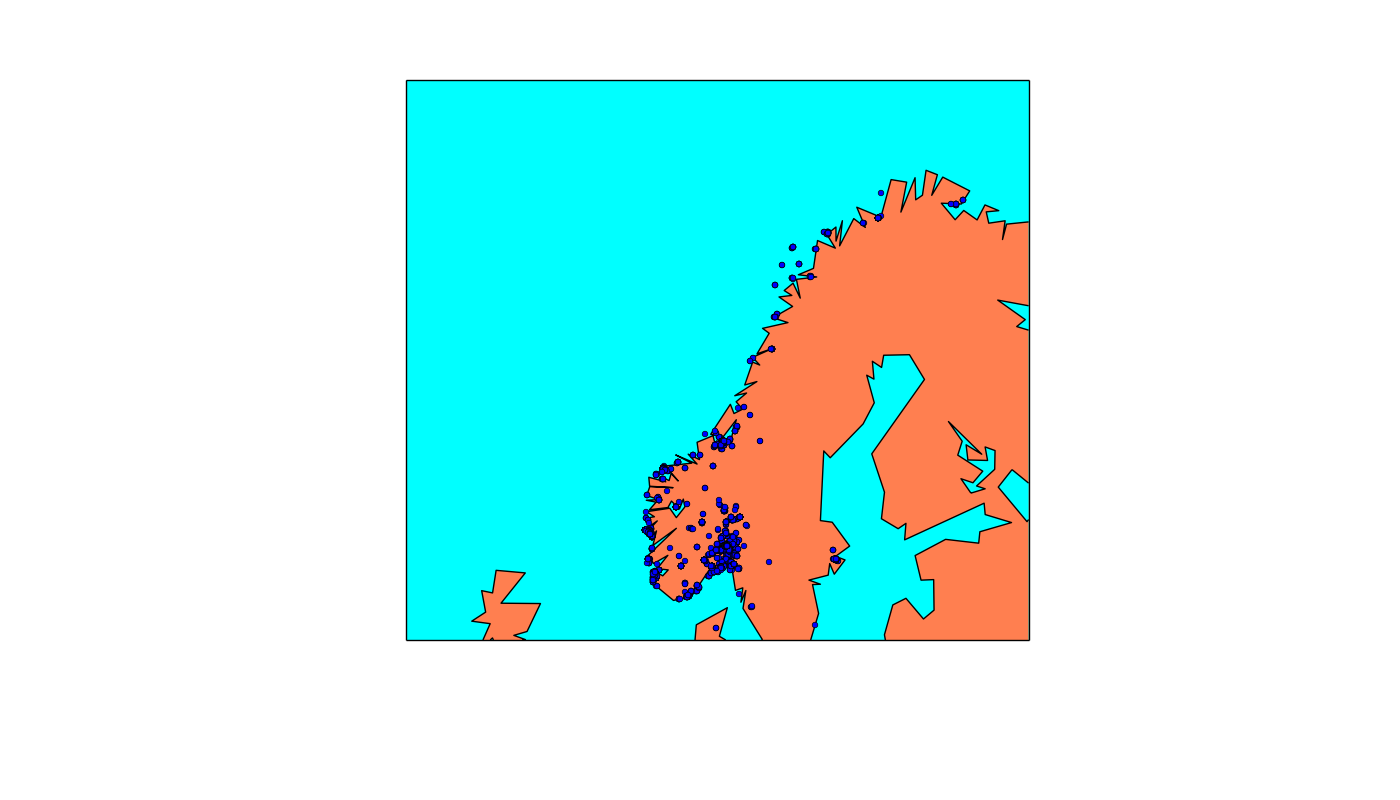
\includegraphics[width=5in]{image/simpleGeoPlotNorway.png}
        \centering
        \caption{Plot of event location in and around Norway}
    \label{figure:croppedGeoplot}
    \end{figure}
        Figure~\ref{figure:croppedGeoplot} shows the location of the user at the time the different events was triggered.
        It is cropped to show events triggered in and around Norway.
        We can see that the majority of the users are located in and around the capital city of Norway, Oslo.

        If the event is triggered from a phone, the event is as precise as the GPS hardware location of the phone, and would be helpful information to understand more about the user.

\subsection{Product properties}
    The properties of the products can tell help to tell how the products are being interacted with, and the distribution of events on them.

    The next two figures presents the distribution of price of the products in the database.

    \begin{figure}[H]
        \centering
        \begin{subfigure}{.5\textwidth}
            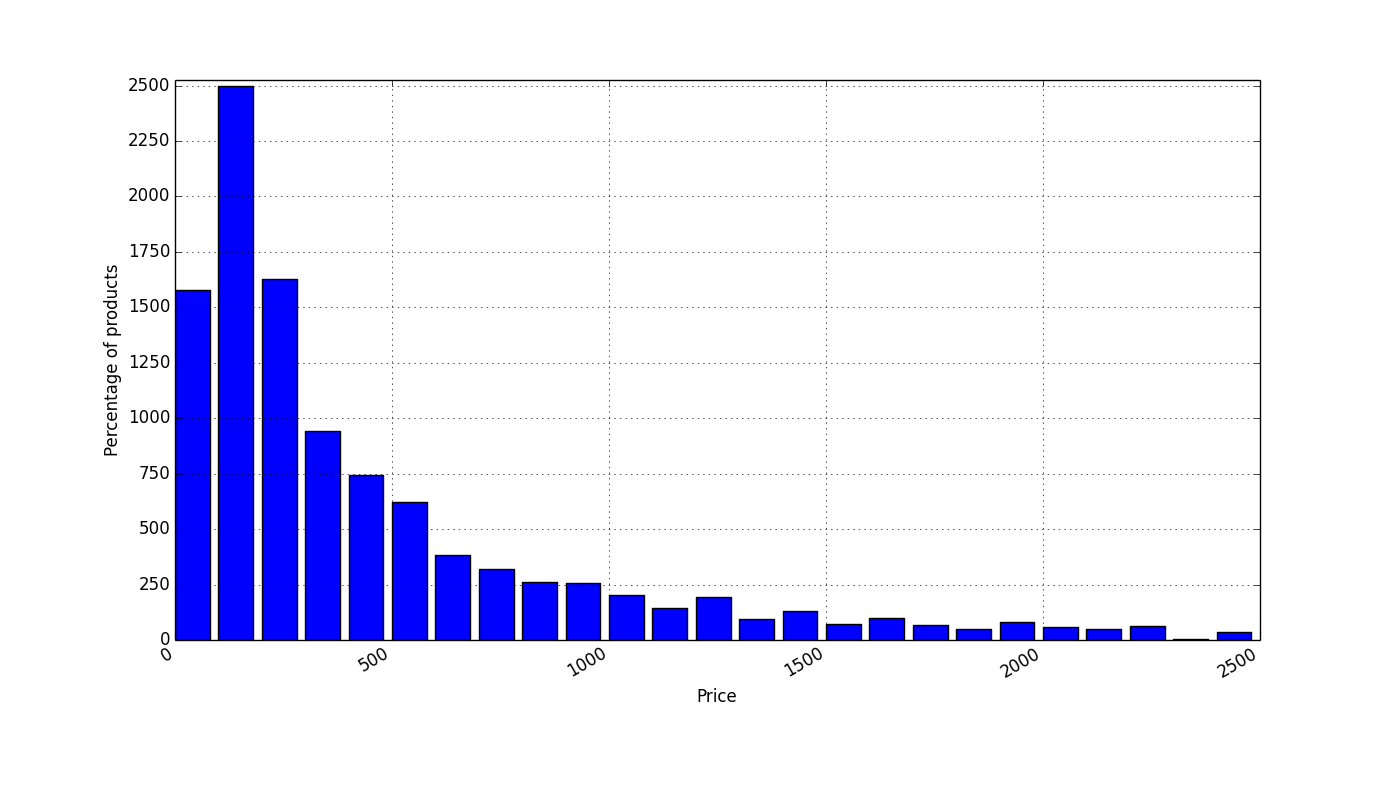
\includegraphics[width=\dualGraphWidth]{image/priceDistributiondistribution.png}
            \centering
            \caption{Price distribution of products}
    \label{figure:pricePerProduct}
        \end{subfigure}%
        \begin{subfigure}{.5\textwidth}
            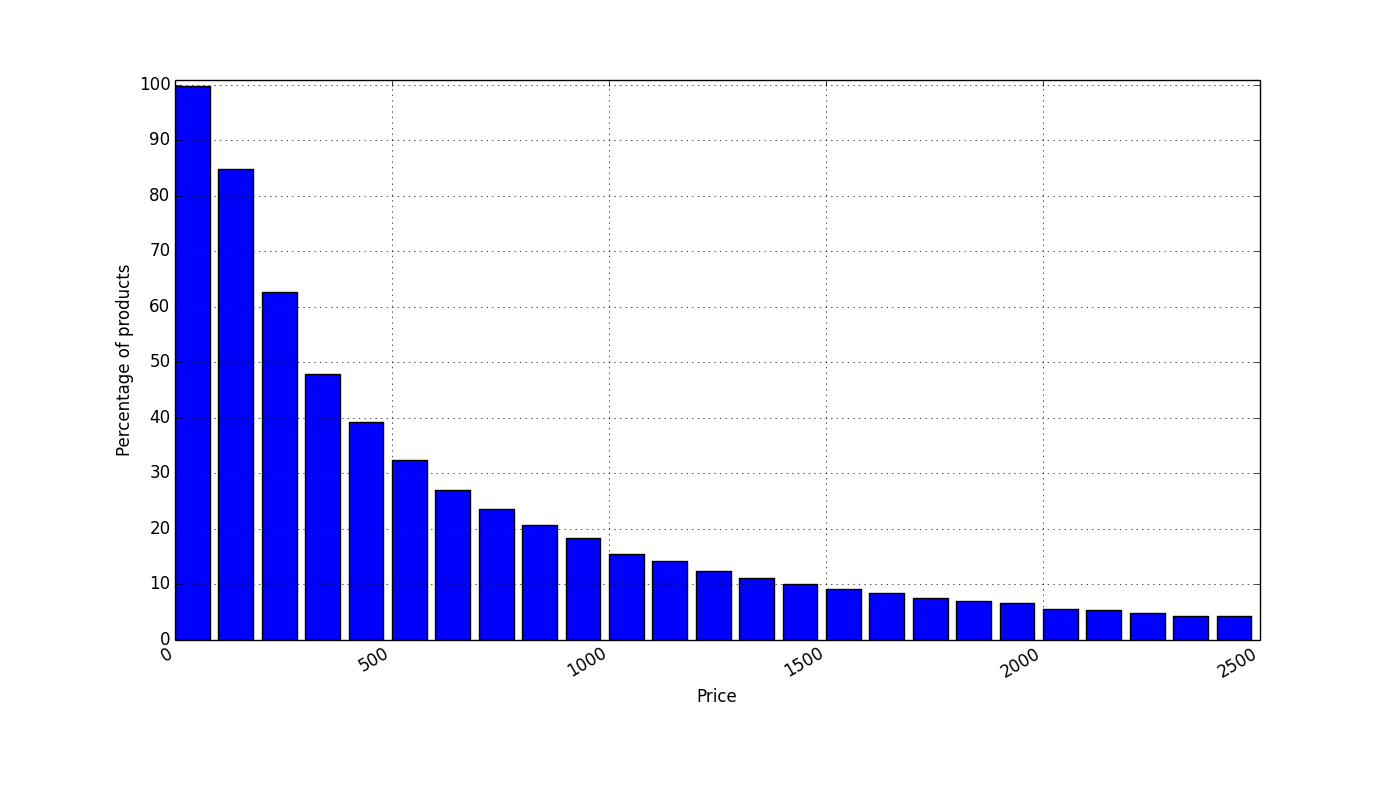
\includegraphics[width=\dualGraphWidth]{image/cumpriceDistributiondistribution.png}
            \centering
            \caption{Cumulative price distribution of products}
    \label{figure:pricePerProductCum}
        \end{subfigure}
        \caption{Figures presenting the distribution of price for the items i SoBazaar}
    \end{figure}
        Here we see how the products are distributed in regards to their price.
        134 of the products have a price over 2 500 NOK and have been left out of this graph.

        The price range of the application varies a lot, but 82\% of the items have a price lower than 1 000 NOK.

        Next figures up are two ways of presenting the distribution of events on the items in the dataset.

    \begin{figure}[H]
        \centering
        \begin{subfigure}{.5\textwidth}
            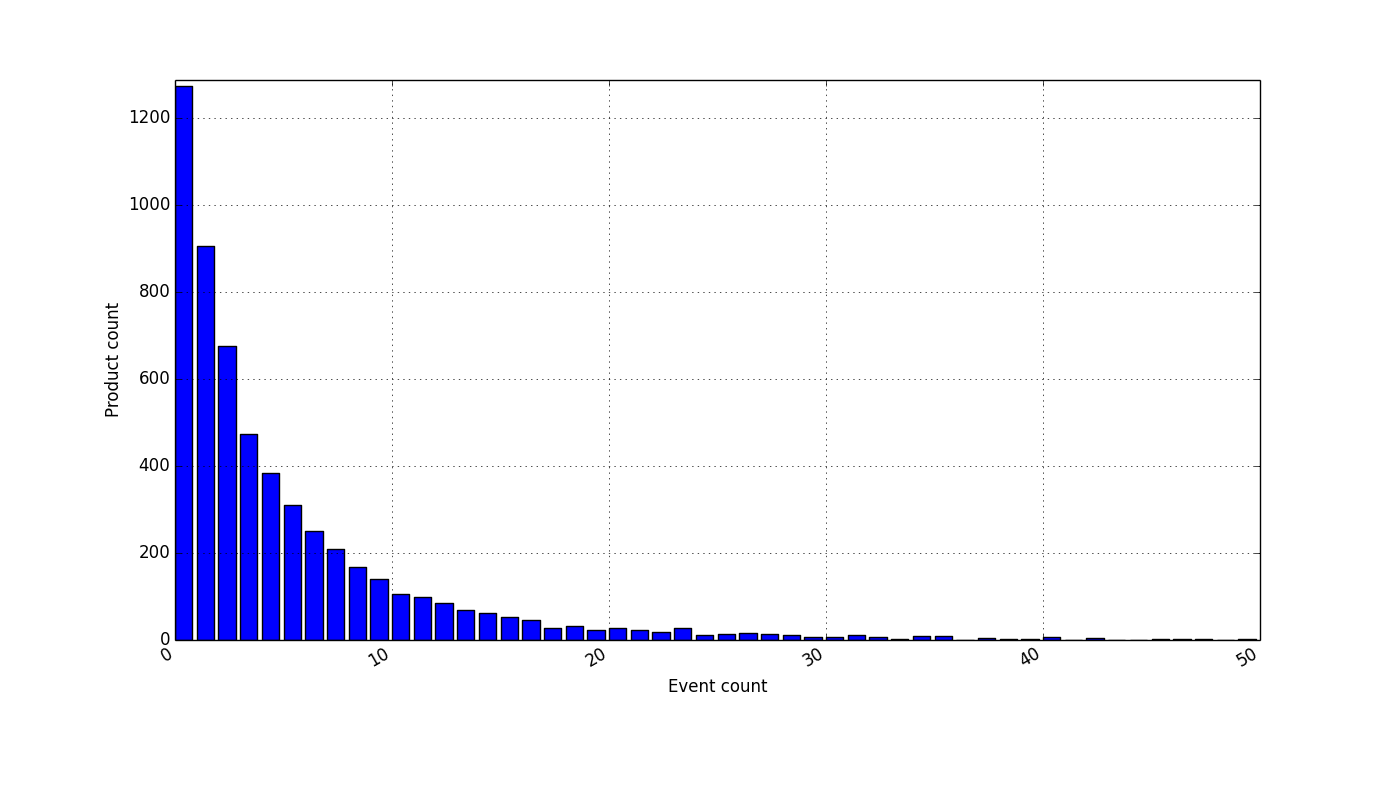
\includegraphics[width=\dualGraphWidth]{image/product_iddistribution.png}
            \centering
            \caption{Count of events on products}
    \label{figure:eventsPerproduct}
        \end{subfigure}%
        \begin{subfigure}{.5\textwidth}
            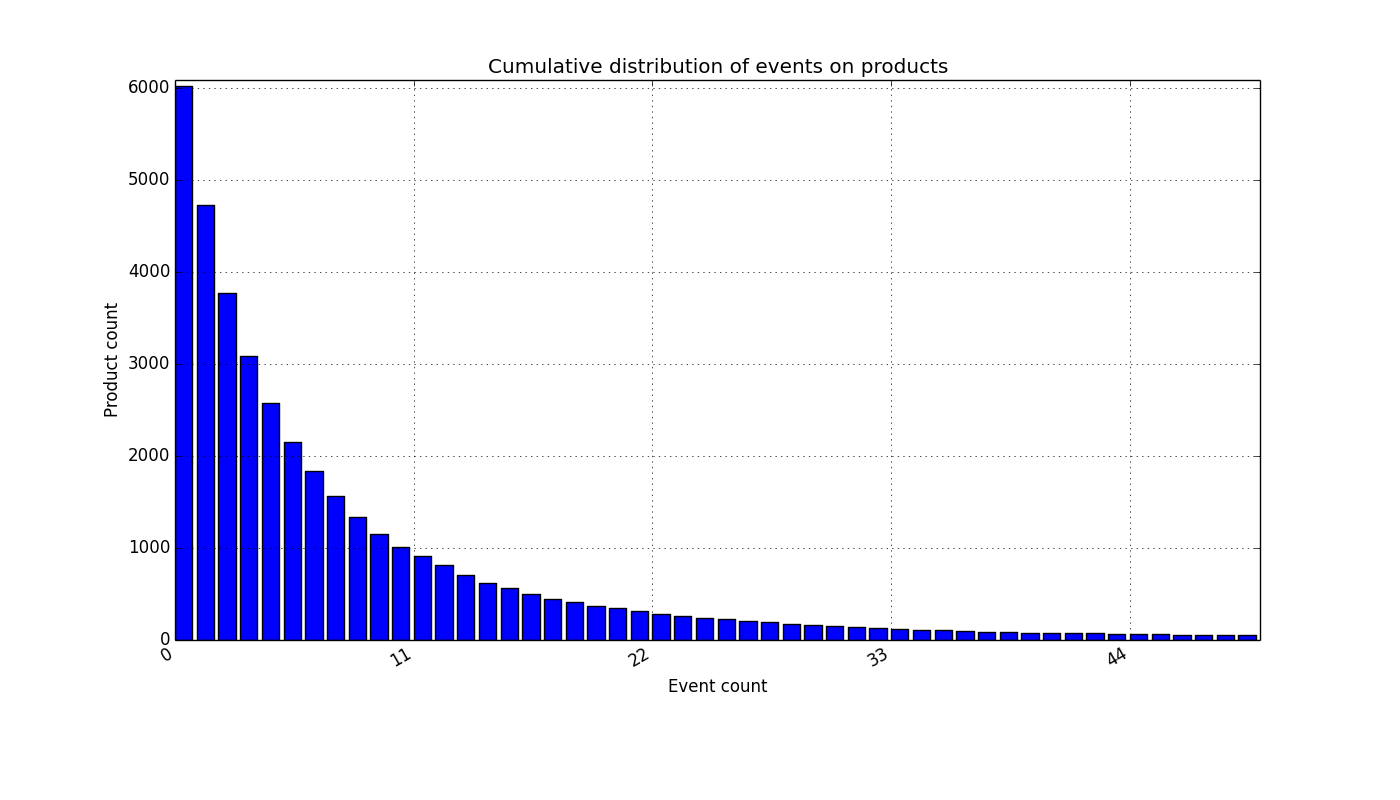
\includegraphics[width=\dualGraphWidth]{image/product_idcumdistribution.png}
            \centering
            \caption{Cumulative count of events on products}
    \label{figure:eventsPerproductCum}
        \end{subfigure}
        \caption{Figures presenting the distribution of events for the products i SoBazaar}
    \end{figure}
        80\% of the products only have an interaction count of 10 or less, where interaction count is \emph{product\_detail\_clicked}, \emph{product\_wanted} and \emph{product\_purchase\_intended}.
        This means that there will not be more than 10 events for the majority of the items, with no more than 10 datapoints to connect with other items for the majority of the items, recommendations done through connecting items to other items through item interaction, might prove problematic.

        When the majority of the events only has 10 events and there are over 6 000 items and 2 000 users, the probability that multiple users have interacted with similar items will be marginal, but promotes the importance of utilizing all the feedback to bolster the recommender.

\subsubsection{The Pareto principle and Long tail on sales}
    In e-commerce the distribution of sales or product interactions can often be described by the Pareto principle and the phenomenon of long tail.
    Pareto's principle is used to tell how the distribution is in the \emph{head}~\footnote{Take for example figure~\ref{figure:eventsPerproduct}, the \emph{head} is the left most part where the curve is steep} of the graph, and the long tail phenomenon is used to tell how the distribution is in the \emph{tail}~\footnote{Take for example figure~\ref{figure:eventsPerproduct}, the \emph{tail} is the right most part where the curve flattens out} of the graph.

\paragraph{Pareto's Principle}
    Pareto's principle applies when the 20\% most frequent products account for more than 80\% of the ratings, sales or interactions in the dataset~\cite{newman05power}.

    \begin{figure}[H]
        \centering
        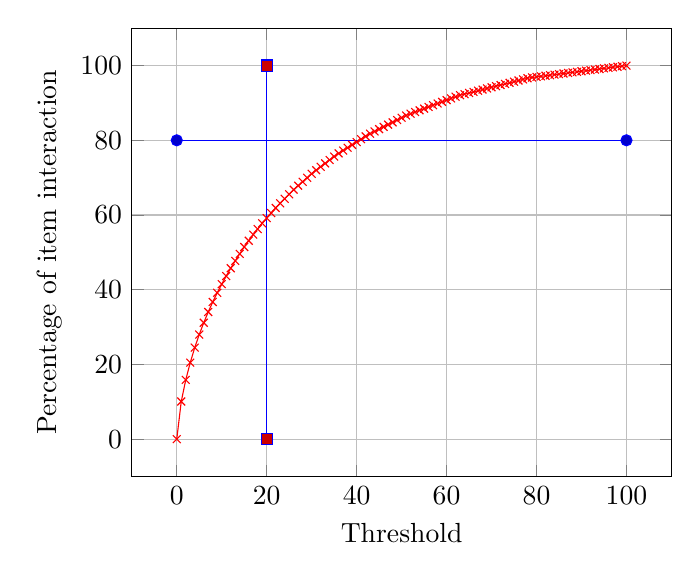
\begin{tikzpicture}
            \begin{axis}[
                xlabel=Threshold,
                ylabel=Percentage of item interaction,
                grid=major,
            ]
            \addplot+[color=blue,sharp plot] coordinates
                {(0,80) (100,80)};
            \addplot+[color=blue,sharp plot] coordinates
                {(20,0) (20,100)};
            \addplot[color=red,mark=x] coordinates {
                    (0.0, 0.0)
                    (1.0, 10.089827139370456)
                    (2.0, 15.879525954256096)
                    (3.0, 20.48914274211811)
                    (4.0, 24.52004126512845)
                    (5.0, 28.004931686083083)
                    (6.0, 31.16775281181592)
                    (7.0, 34.053795636967514)
                    (8.0, 36.72848048712981)
                    (9.0, 39.184258863196035)
                    (10.0, 41.49409958986488)
                    (11.0, 43.66303499987419)
                    (12.0, 45.76151775155373)
                    (13.0, 47.72412751931158)
                    (14.0, 49.60370379689505)
                    (15.0, 51.44553757894472)
                    (16.0, 53.116272047907806)
                    (17.0, 54.75178018770601)
                    (18.0, 56.2614800090582)
                    (19.0, 57.79634149409959)
                    (20.0, 59.17016833153008)
                    (21.0, 60.52889817074705)
                    (22.0, 61.887628009964025)
                    (23.0, 63.14571119442417)
                    (24.0, 64.35347105150593)
                    (25.0, 65.56123090858767)
                    (26.0, 66.78912009662079)
                    (27.0, 67.84842613793623)
                    (28.0, 68.90521601288278)
                    (29.0, 69.9620058878293)
                    (30.0, 71.03640892735828)
                    (31.0, 72.00261681302368)
                    (32.0, 72.90843670583499)
                    (33.0, 73.8142565986463)
                    (34.0, 74.73517348967114)
                    (35.0, 75.64099338248245)
                    (36.0, 76.49900611428427)
                    (37.0, 77.25385602496037)
                    (38.0, 78.02128676748107)
                    (39.0, 78.77613667815716)
                    (40.0, 79.53098658883326)
                    (41.0, 80.29841733135395)
                    (42.0, 81.05326724203005)
                    (43.0, 81.77540698991017)
                    (44.0, 82.37928691845104)
                    (45.0, 82.9932315124676)
                    (46.0, 83.59711144100848)
                    (47.0, 84.20099136954934)
                    (48.0, 84.80487129809023)
                    (49.0, 85.41881589210678)
                    (50.0, 86.02269582064767)
                    (51.0, 86.62657574918853)
                    (52.0, 87.11974435749693)
                    (53.0, 87.57265430390258)
                    (54.0, 88.02556425030824)
                    (55.0, 88.47847419671389)
                    (56.0, 88.9389326422263)
                    (57.0, 89.39184258863196)
                    (58.0, 89.84475253503761)
                    (59.0, 90.29766248144327)
                    (60.0, 90.75812092695568)
                    (61.0, 91.21103087336134)
                    (62.0, 91.66394081976699)
                    (63.0, 92.06149510605641)
                    (64.0, 92.36343507032684)
                    (65.0, 92.66537503459729)
                    (66.0, 92.96731499886772)
                    (67.0, 93.27428729587601)
                    (68.0, 93.57622726014644)
                    (69.0, 93.87816722441687)
                    (70.0, 94.18010718868732)
                    (71.0, 94.48707948569559)
                    (72.0, 94.78901944996603)
                    (73.0, 95.09095941423647)
                    (74.0, 95.39289937850691)
                    (75.0, 95.69987167551518)
                    (76.0, 96.00181163978563)
                    (77.0, 96.30375160405606)
                    (78.0, 96.61072390106435)
                    (79.0, 96.8170495433158)
                    (80.0, 96.96801952545103)
                    (81.0, 97.11898950758624)
                    (82.0, 97.27247565609038)
                    (83.0, 97.4234456382256)
                    (84.0, 97.57441562036082)
                    (85.0, 97.72538560249603)
                    (86.0, 97.87887175100018)
                    (87.0, 98.0298417331354)
                    (88.0, 98.18081171527061)
                    (89.0, 98.33429786377475)
                    (90.0, 98.48526784590997)
                    (91.0, 98.6362378280452)
                    (92.0, 98.7872078101804)
                    (93.0, 98.94069395868455)
                    (94.0, 99.09166394081976)
                    (95.0, 99.24263392295498)
                    (96.0, 99.3936039050902)
                    (97.0, 99.54709005359435)
                    (98.0, 99.69806003572957)
                    (99.0, 99.84903001786478)
                    (100.0, 100.0)
            };
            \end{axis}
        \end{tikzpicture}
        \caption{Pareto's principle values graphed}
    \label{figure:paretosPrinciple}
    \end{figure}

    \begin{table}[H]
        \centering
        \begin{tabular}{lll}
        \toprule
        Threshold &   Products in threshold~\tablefootnote{\label{footnote:pt}The amount of products residing within the percentage threshold} &      Percentage of interactions \\
        \midrule
        20\%    &    1206   &    59.1701\% \\
        41\%    &    2472   &    80.2984\% \\
        \bottomrule
        \end{tabular}
        \caption{Pareto's principle values}
    \label{table:paretosPrinciple}
    \end{table}

    Figure~\ref{figure:paretosPrinciple} show the percentages of interactions within the given thresholds.
    As we can see from table~\ref{table:paretosPrinciple}, the 20\% most frequently interacted with items represents 59.1701\% of the item interaction in total.
    We have to move up to 41\% to reach 80\% of the interactions, and the Pareto's principle does therefore not apply to the SoBazaar dataset.

    Even though Pareto's Principle does not apply to this data, is the information regarding where the majority (the 80\%) of the item interaction resides valuable.
    To reach the majority of the item interaction we have to cover over 41\% of the most popular items, which might in turn lead to bad most popular results.

\paragraph{Long Tail}
    The definition of long tail is that the most frequently-occurring items represent less than 50\% of occurrences in logs~\cite{DBLP:journals/corr/abs-1203-4487}.

    \begin{table}[H]
        \centering
        \begin{tabular}{llll}
        \toprule
        Average product interaction   & Products in threshold~\tablefootnote{See footnote~\ref{footnote:pt}} & Coverage & Percentage of interactions \\
        \midrule
        6.6928   &    4194   & 68.8443\% &   28.5408\% \\
        \bottomrule
        \end{tabular}
        \caption{Long tail values}
    \label{table:longtail}
    \end{table}

    As the table above shows the SoBazaar data does not posses a clear long tail behavior.
    The average interaction count of the products is 6.6928 and there is 4194 products with less than this number of interactions, but these items does only cover 28.5408\% of the total interactions.

    The next figure displays an overview of which events are triggered on the \emph{storefronts} in the SoBazaar application.

    \begin{figure}[H]
        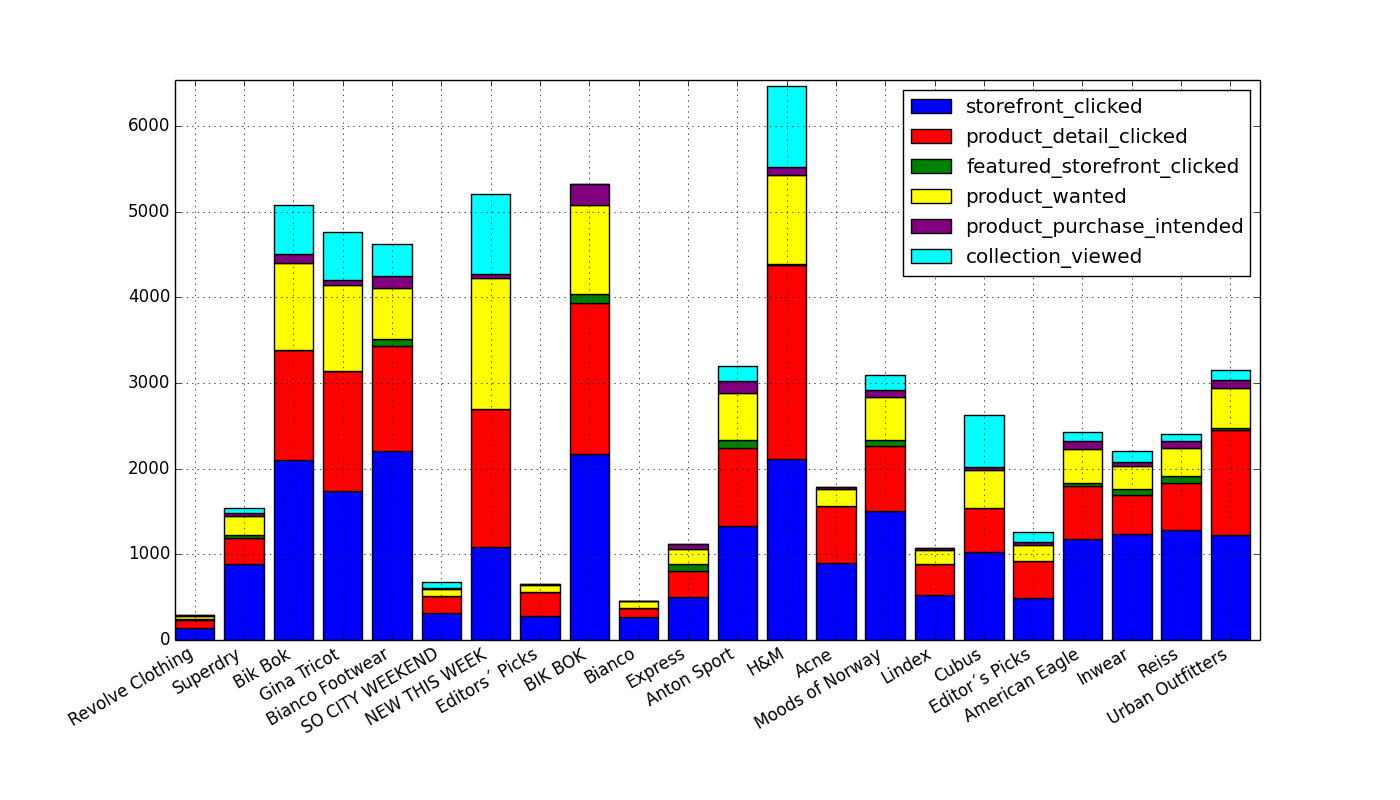
\includegraphics[width=5in]{image/storefront_nameandEventdistribution.png}
        \centering
        \caption{Distribution of events on storefronts}
    \label{figure:eventOnStoreFrontDist}
    \end{figure}
        The figure above presents the event distribution on the different storefronts.
        The events are segmented to show the different event counts on the different storefronts, and stacked to show the complete count, to be able to clearly see how the events are distributed over the different stores.
        We can see that \emph{H\&M} is the most popular store in total, but \emph{BIK BOK} has the most \emph{product\_purchase\_intended}-events.
        One interesting find to take from this graph is the \emph{storefront\_clicked} to the item interaction related events (\emph{product\_detail\_clicked}, \emph{product\_wanted} and \emph{product\_purchase\_intended}) ratio.
        For instance \emph{Bik Bok} has a much higher item interaction count than storefront access count, whereas stores such as \emph{Reiss} and \emph{Inwear} are mostly accessed and the items not interacted with.
        Different aspects affecting this might be price, style and item presentation.

\subsection{Time properties}
    It is not only important to look at if a user has accessed an item, or if a user has a certain preference, time might also tell something about the preferences of the user.

    The next figure shows the average lifetime of the products in the SoBazaar database.

    \begin{figure}[H]
        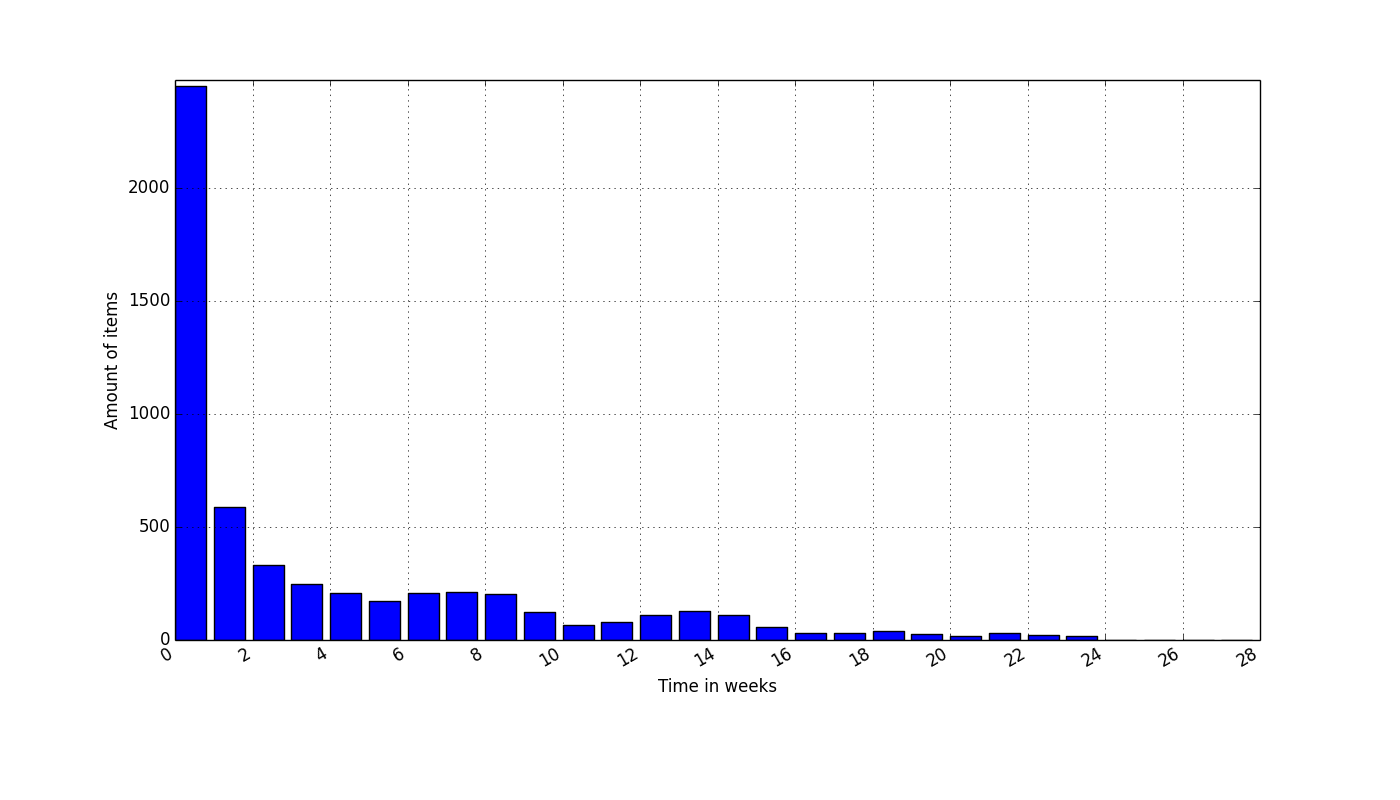
\includegraphics[width=5in]{image/itemTimespansdistribution.png}
        \centering
        \caption{Count of the different time spans of the items}
    \label{figure:itemLifes}
    \end{figure}
        This figure shows the count of products which has the different time spans.
        This figure makes it clearer than figure~\ref{figure:itemTimeSpanEventCount} how long the majority of the the products have lived.

        Almost 2 500 products have a life span of less than a week, which shows how important it is to handle the recentness of the products to be able to follow the ever-changing trends.

        Including the amount of item interactions mapped together with the lifespan of the items is the next figure up, to better see how the lifespan of the items change with the amount of item interactions on them.

    \begin{figure}[H]
        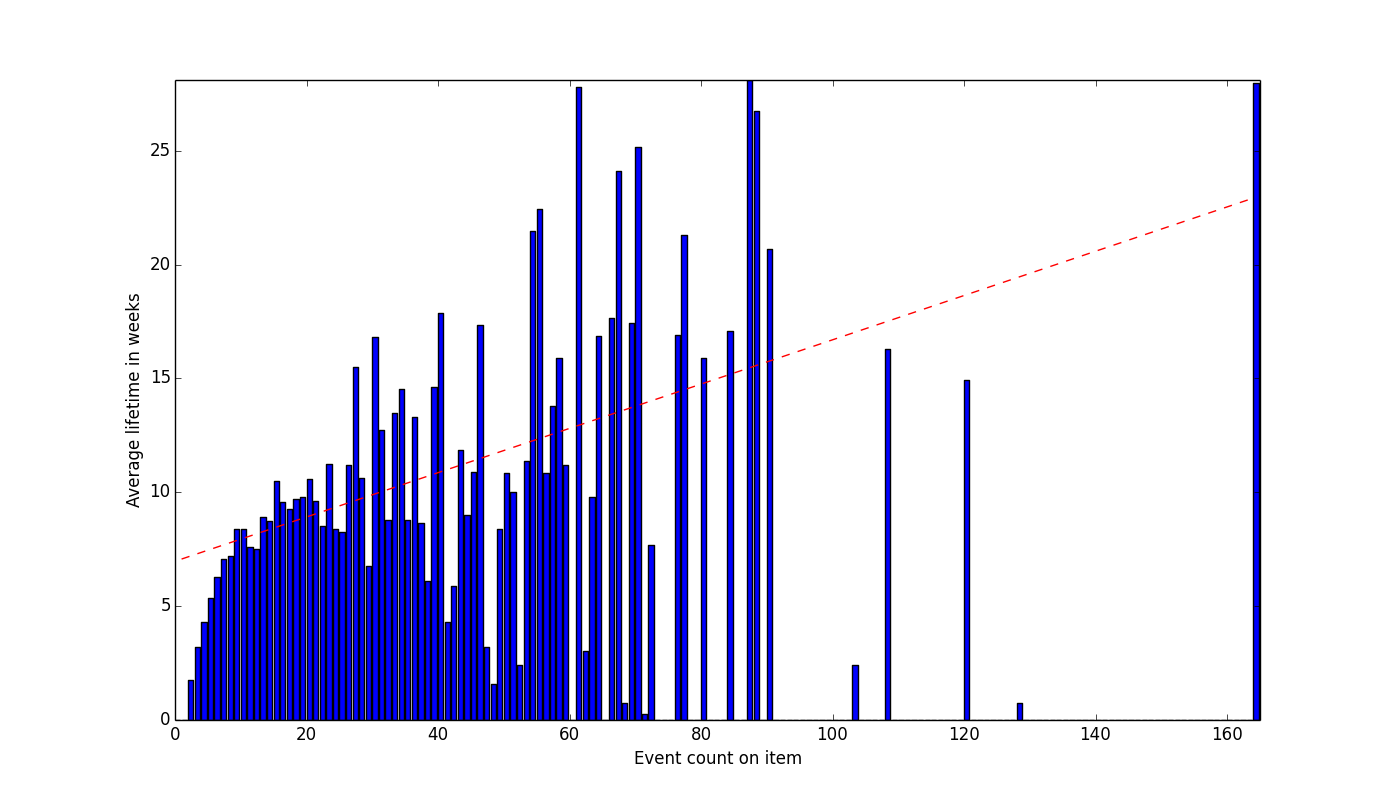
\includegraphics[width=5in]{image/avglifetimeoncount.png}
        \centering
        \caption{Average life time of products grouped on event count}
    \label{figure:averageLifetimBasedoncount}
    \end{figure}
        This figure shows the life span of the products grouped and sorted on the number of interactions on the items.
        The life span of an item is the time from the first event on the item till the last event on the item.
        The red line is the regression line of the average life spans at the different interactions counts.
        The gap between 117 to 160 is because no items have an interaction count of that amount.

        As we can see from the regression line, the average life span of an item increases with the count of item interactions, which is somewhat expected since they are in many ways intertwined, but there are indications of a reduction of interest with time, which advocates the idea that recentness is important.

        The figure above averaged the lifespan of the items and presented them with together with their respective count, the next figure keeps them separate, to not lose the lifespan distribution.

    \begin{figure}[H]
        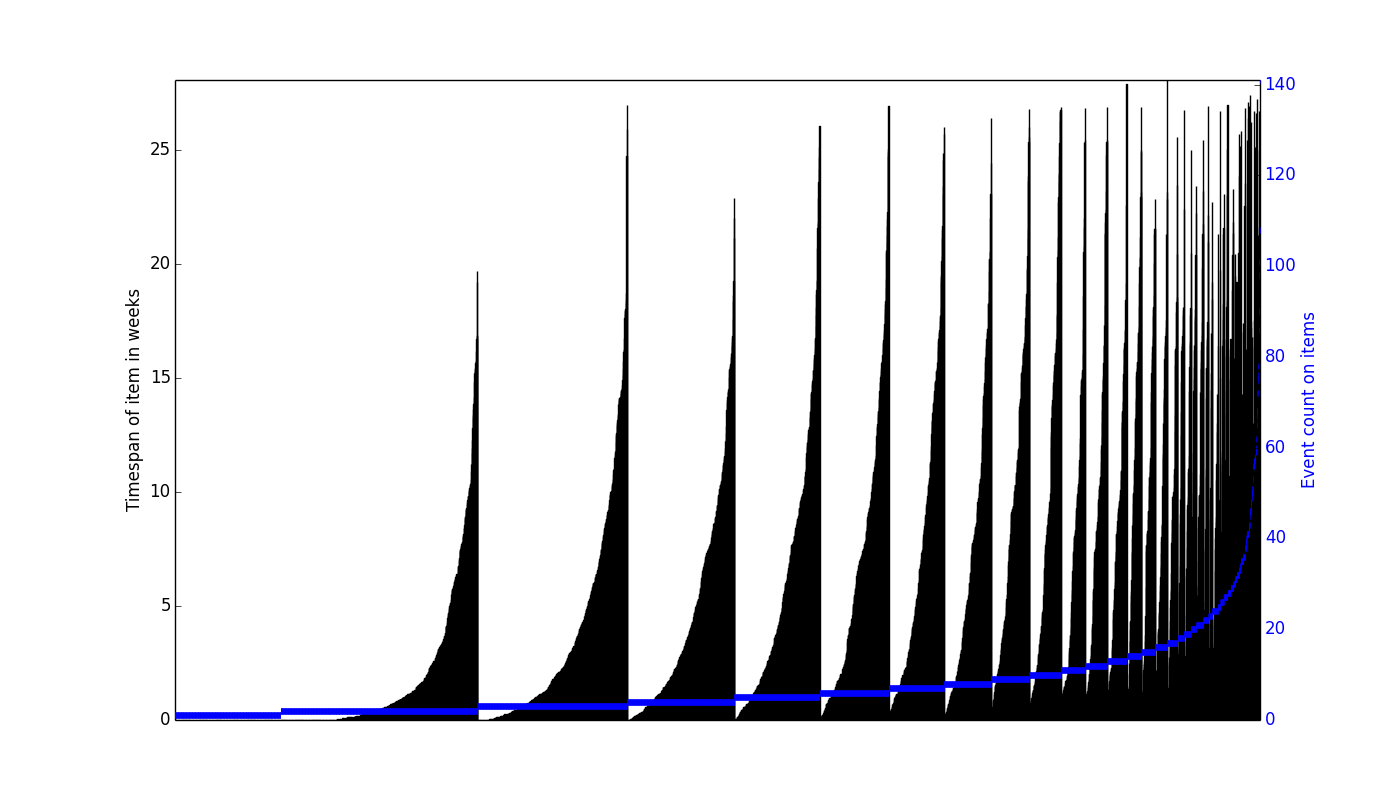
\includegraphics[width=5in]{image/itemTimeSpansortedoneventcount.png}
        \centering
        \caption{Life time of items mapped with event count}
    \label{figure:itemTimeSpanEventCount}
    \end{figure}
        This figure shows the total life span of each item mapped together with the amount of events triggered on them.
        As mentioned earlier, the life span of an item is the time since the first event on the item till the last event on the item.
        This figure is showing the same data as in figure~\ref{figure:averageLifetimBasedoncount}, but instead of taking the average life span at the give product interactions count, the products are mapped separately, to show the diversity in life span given the different product interaction counts.

        Time is shown in weeks, so the longest time span of an item is about 27 weeks, which is close to the time span of the events gathered from SoBazaar.
        Even though an item has a long time span does not mean that the item has been of measurable interest to the users in the SoBazaar application, but we see that the more interaction on the item, the longer the average life time, but the recentness of an item is important.
        Even though some item has a lot of interaction, they item can have a quite low lifespan, which promotes the importance of looking into recentness.

        Next figures presents how long in average the user use before taking an action such as \emph{purchase} or \emph{want}.

    \begin{figure}[H]
        \centering
        \begin{subfigure}{.5\textwidth}
            \centering
            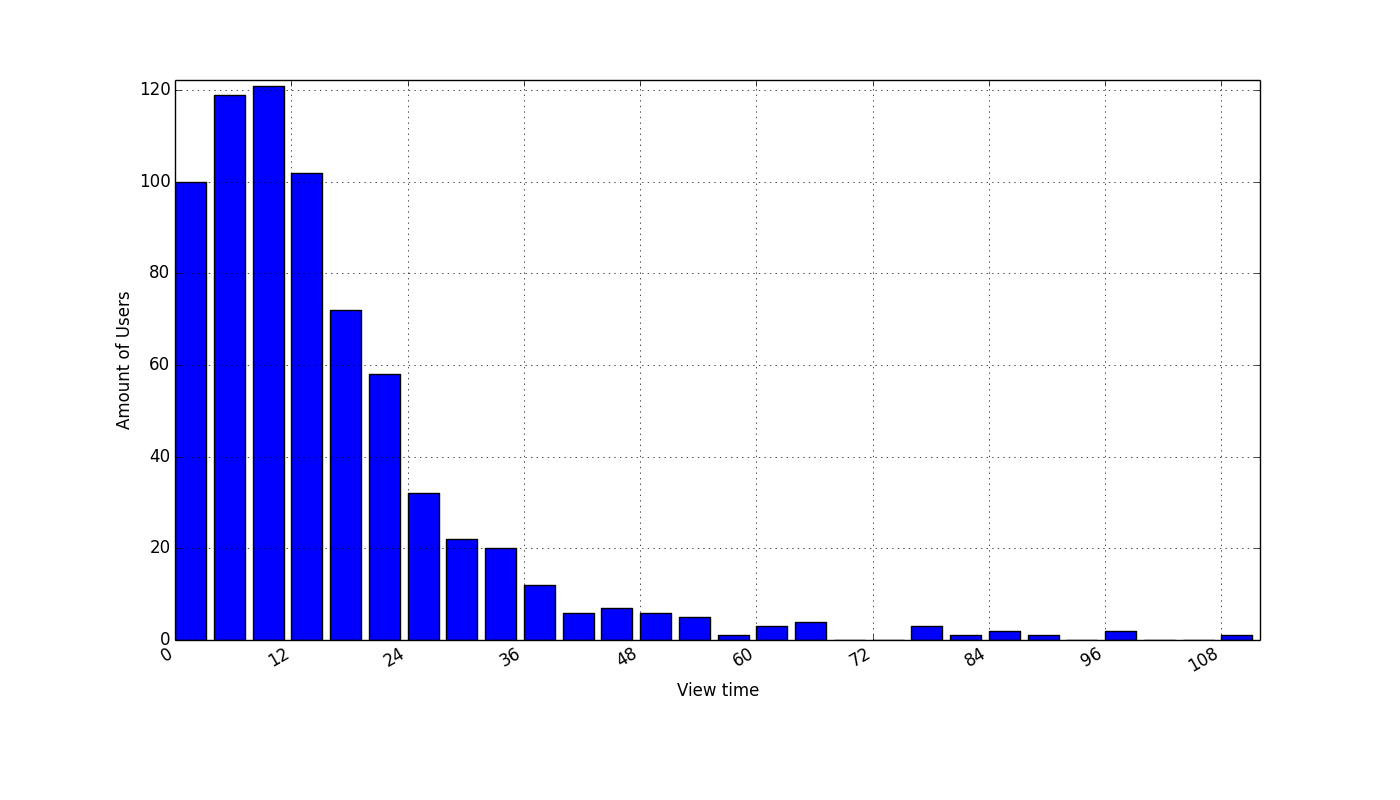
\includegraphics[width=\dualGraphWidth]{image/product_wanteddistribution.png}
            \caption{View times before wanting an item}
    \label{figure:viewWant}
        \end{subfigure}%
        \begin{subfigure}{.5\textwidth}
            \centering
            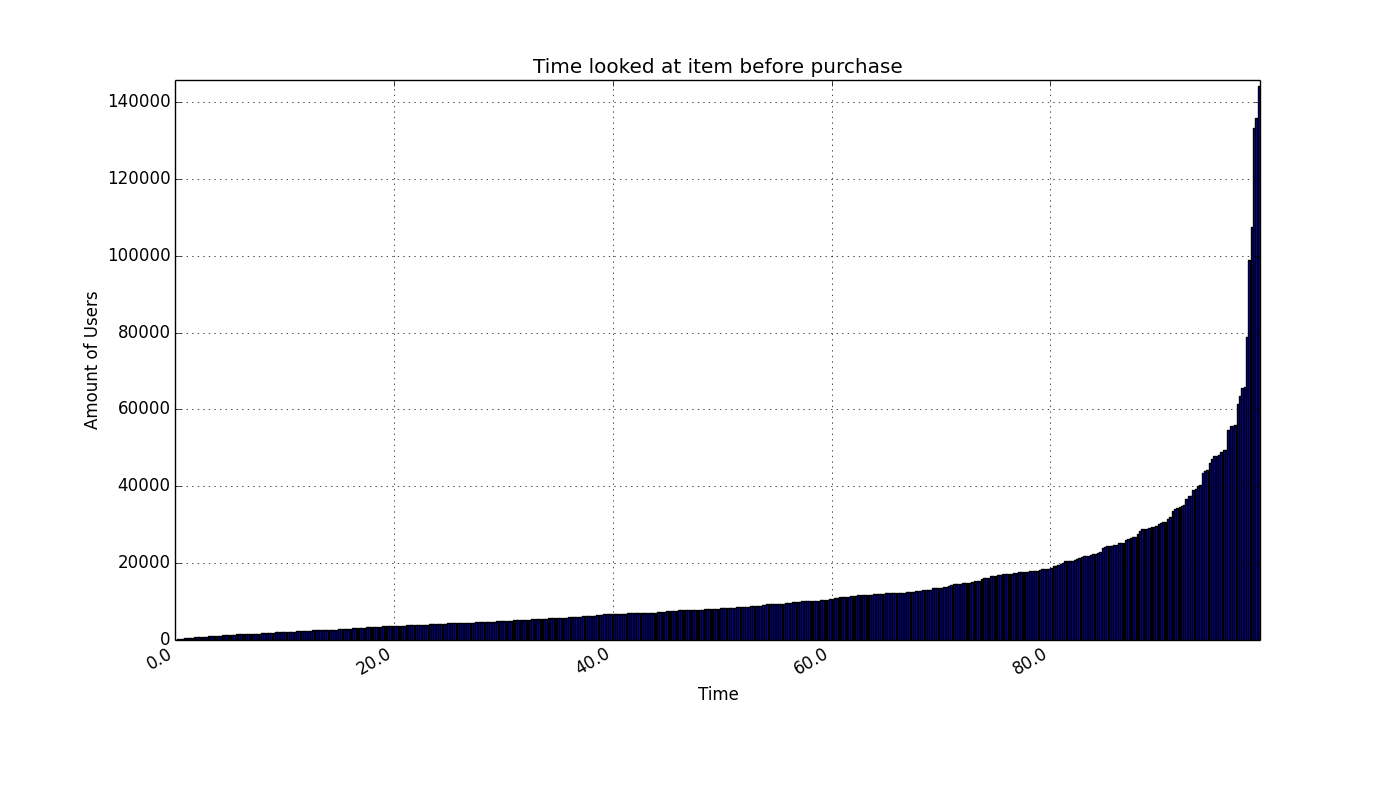
\includegraphics[width=\dualGraphWidth]{image/product_purchase_intendeddistribution.png}
            \caption{View times before purchasing an item}
    \label{figure:viewBuy}
        \end{subfigure}
        \caption{Average view times of products before want or purchase}
    \end{figure}
        The figures above shows the average time of the users of the SoBazaar application before pressing either \emph{want} or \emph{purchase}.

        The average times between the two are quite similar, but we can see that the user is on average somewhat faster to press \emph{purchase}.
        The data set on \emph{product\_purchase\_intended} is considerably smaller than \emph{product\_wanted}, so the trends seen here are inconclusive at best.

        The figures above presented the actions \emph{purchase} and \emph{want}, the next figure presents the \emph{bounce rate}, or in other words, how fast the user on average triggered a non related event to the item currently being watched.
    \begin{figure}[H]
        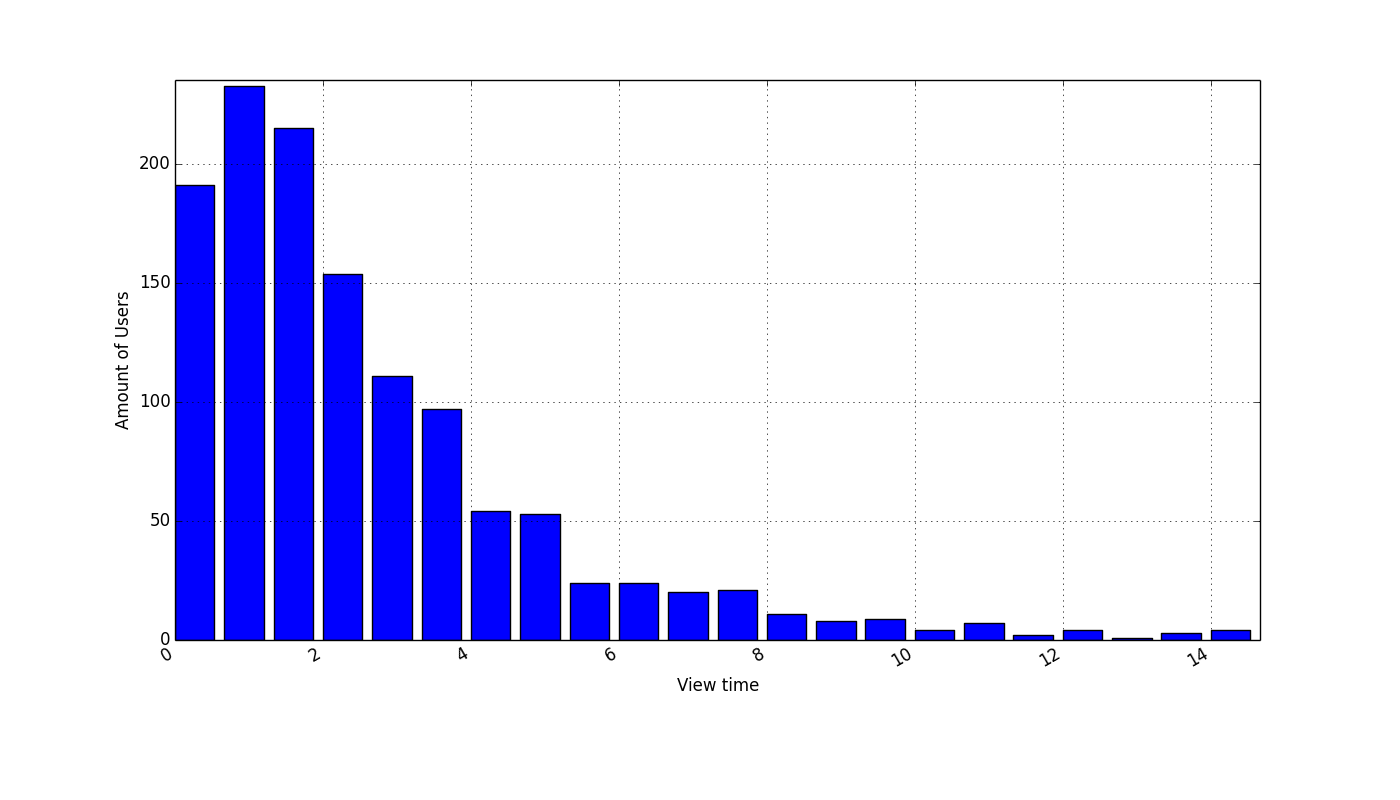
\includegraphics[width=5in]{image/product_detail_clickeddistribution.png}
        \centering
        \caption{View times before leaving an item (Bounce Rate)}
    \label{figure:bounceRate}
    \end{figure}
        This figure shows the time the users use before not taking any more action towards the item (\emph{purchase} or \emph{want}).
        The majority of the users have a view time of less than 6 seconds before they moves on to another item.

        When comparing this figure with figure~\ref{figure:viewWant} and figure~\ref{figure:viewBuy} we see a more definite difference.
        The users are much faster to look at a new item when not pressing \emph{want} or \emph{purchase}.
        This could indicate a disinterest towards the item.

    \begin{figure}[H]
        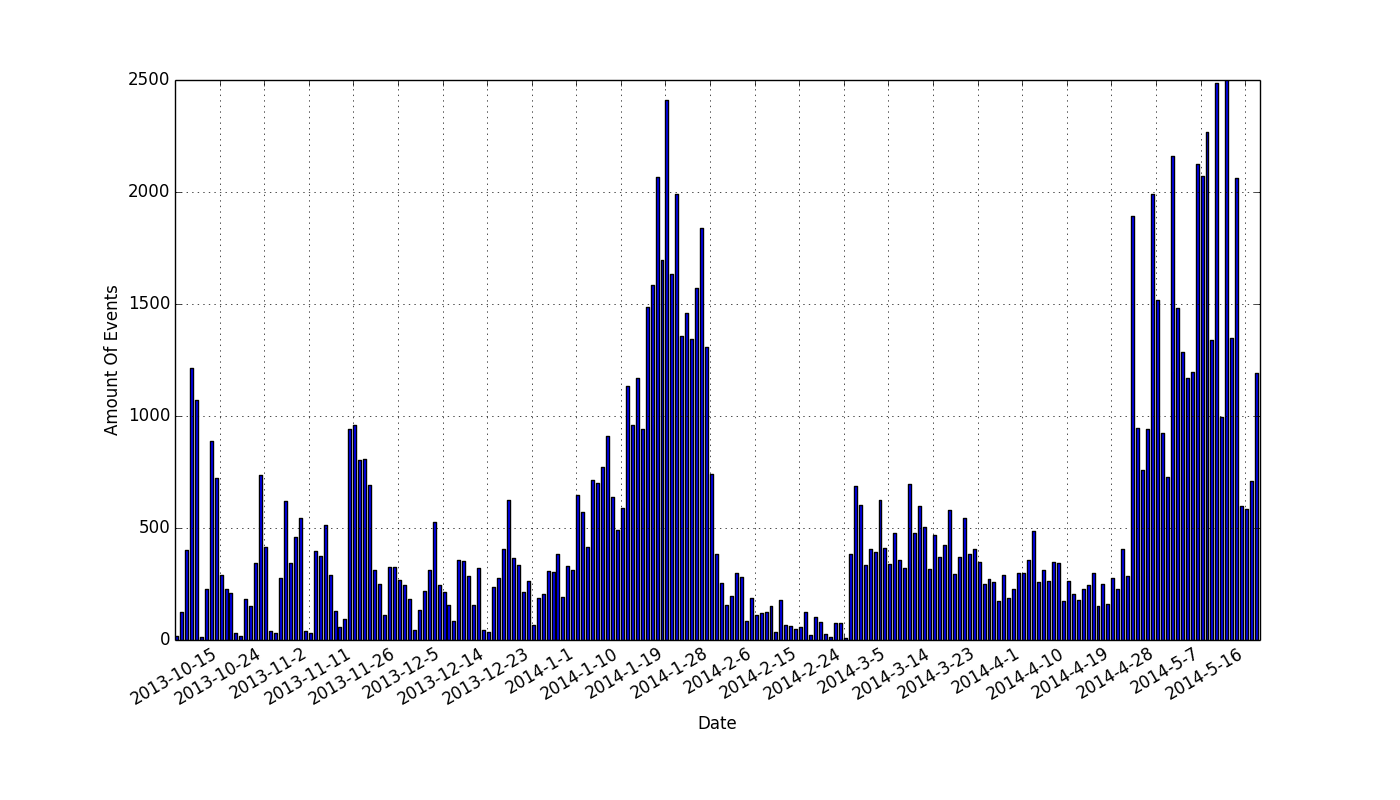
\includegraphics[width=5in]{image/eventsPerDay.png}
        \centering
        \caption{Distribution of events per day}
    \label{figure:eventOnDaysDist}
    \end{figure}
        This figure shows the event distribution per day over the time period the events were stored.
        The spikes we see happens on a weekly basis, and is centered around the weekends, which is natural since this is an entertainment applications.
        The larger spike from the start of January to the start of March and end of April to the end of May might be due to increase in publicity or other outside factors.

   \begin{figure}[H]
        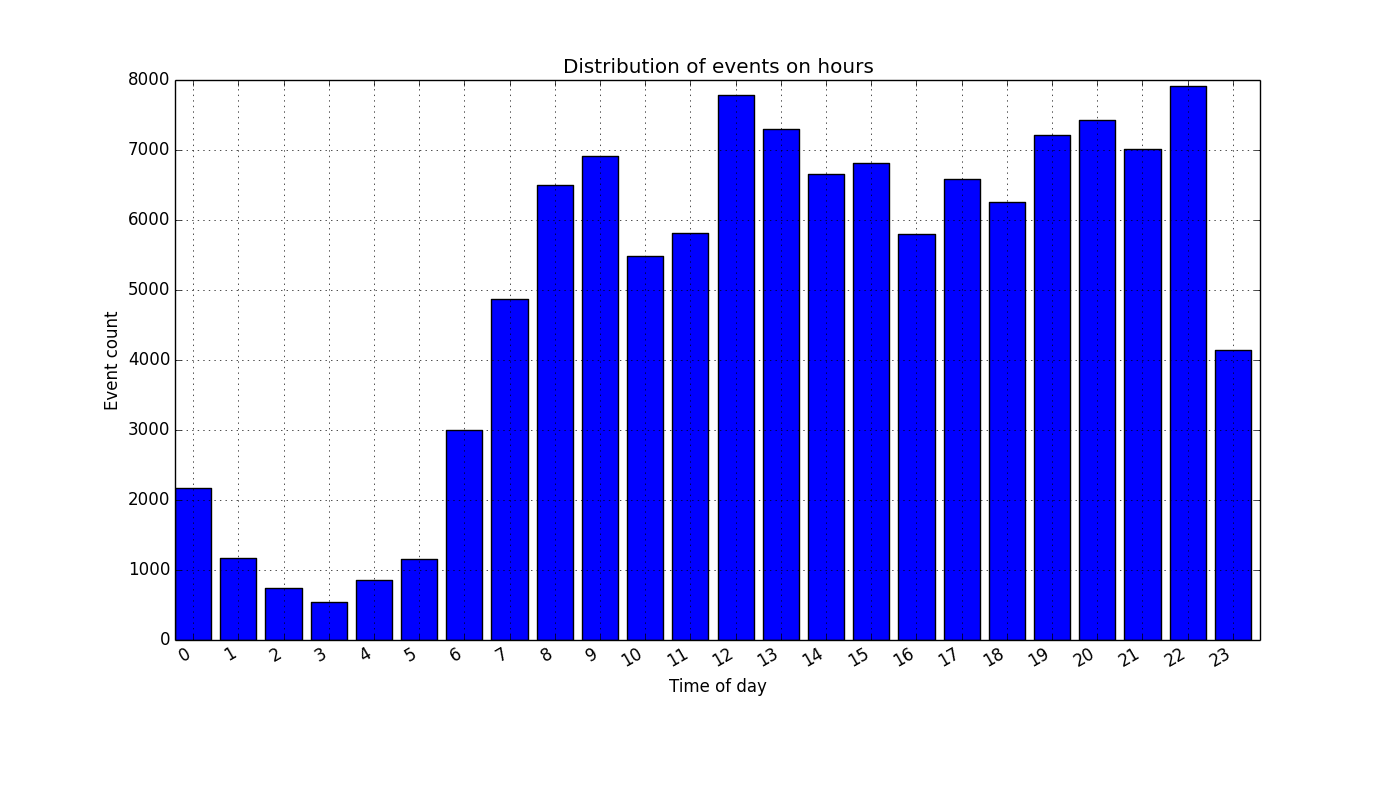
\includegraphics[width=5in]{image/hrdistribution.png}
        \centering
        \caption{Events at time of day}
    \label{figure:timeOfDayDistr}
    \end{figure}
        The figure above presents the amount of events during the given hours.

        One interesting discovery from this figure is the shape. One might have expected the application usage to have a sinus wave shape, but it has instead an increase in usage around 22 o'clock, which support the claim done based on figure~\ref{figure:eventOnDaysDist}, that SoBazaar is an entertainment application.

\subsection{Discussion}
    The repetitive pattern though out the preceding subsections is that the data is sparse, with low life span of user accounts and items, which is no surprise since the application as a product is in such an early stage.
    This sparsity must be handled to be able to make good recommendations, since it is so central when it comes to making predictions.

    Throughout the data exploration section we also saw that time plays a central role, in context of life span and the users and the items.
    The time an item lives varies greatly, but over one third of the items are active for no more than 1 week, which makes it important to consider how new an item is when making predictions.


\section{Conversion Rate Properties}
\label{sec:conv-rate}

In many domains the number of activities on an item given a specific user
implies preference. The activity in question may be the number of plays in a
music service~\cite{parra2011walk} or the amount of minutes used watching a
specific TV-show~\cite{study-on-implicit-tv}. We want to validate this
hypothesis in the SoBazaar data, determining if the \textit{number of clicks}
on an item implies higher preference, that is an higher probability of buying
the item.

If the hypothesis holds true, we can use this fact in order improve
classification of our models in future sections. In addition we can customize
the user interface so that if a user has clicked the item, we should with a
higher frequency show the item to the user -- as he/she is more probable of
buying it once seen in detail.

In order to validate the hypothesis we iterate through all users and look at
their respective events, summarizing the number of times the user has clicked
an item $n$ times and of these how many times the user also bought it. We do
this for all values of $n$, where $n \in [1,6]$ and obtain the following table
of conversion rates and standard errors.

\begin{table}[H]
  \centering
  \begin{tabular}{lllll}
    \toprule
    N & Clicks & Purchases & Rate & Standard Error \\
    \midrule
    1 & 15602 & 1039  & 0.0667 & 0.20\% \\
    2 & 2672  & 323   & 0.1208 & 0.63\% \\
    3 & 433   & 84    & 0.1939 & 1.89\% \\
    4 & 173   & 36    & 0.2081 & 3.10\% \\
    5 & 65    & 19    & 0.2923 & 5.63\% \\
    6 & 54    & 20    & 0.3703 & 6.57\% \\
    \bottomrule
  \end{tabular}
  \label{tab:prob-purchase}
  \caption{Probabilties of purchase, given $N$ visits on item}
\end{table}

The standard error gives a useful indication on how certain we can be that the
results are statistically significant, and is calculated based on the sample
size (number of clicks) and the amount of conversions. Given the rate as $r$
and sample size as $S$ we calculate the standard error $e$ as:

\begin{equation}
  e = \sqrt{\frac{r(1 - r)}{S}}
\end{equation}

Using the standard error we want to perform an hypothesis test determining if
the results are significant within our accepted confidence of 95\%. In other
words we want to be 95\% sure that the patterns found in the data are not just
random. Our two hypothesis which we want to test are thus:

$\mathbf{H_0:}$ The differences in conversion rates between our first
(baseline) and second scenario is random.

$\mathbf{H_1:}$ The difference is significant, such that one scenario have a
higher probability of conversion.

and we want to do multiple tests when $n \in [2,6[$, using $n-1$ as baseline
and $n$ as the second scenario. For each test we calculate the
\textit{P-value}, which is the probability of obtaining a result at least as
extreme as the one that was actually observed. When the P-value becomes less
that our predetermined significance level ($0.05$ when we do a 95\%
significance test) we can reject our null-hypothesis, which is what we want to
do. In order to find this P-value we use the Standard Score, also called the
\textit{Z-score}, which is the number of standard deviations an observation is
above the mean. As we have two samples we can calculate the difference in
conversion rates and use the cumulated standard error in order to find the
Z-score:

\begin{equation}
  \label{eq-z-score}
  Z = \frac{r_b - r_v}{\sqrt{e_{b}^{2} + e_{v}^{2}}}
\end{equation}

where $r_b$ and $r_v$ are the conversion rates for the baseline and second
scenario respecivly. $e_b$ and $e_v$ are equally the standard errors for the
two scenarios. Using standard normal deviate (normallly distributed random
variable with expected value 0 ($s$) and standard deviation 1 ($h$)) we can
find the cumulative probability for validity of the model - the P-value.

We calculate the P-value using $n=1$ as baseline and $n=2$ as our second
scenario. The Z-score is calculated by Equation~\ref{eq-z-score} and we obtain
our result:

\begin{equation}
  Z = \frac{0.0667-0.1208}{\sqrt{0.0020^2 + 0.0063^2}} = \frac{-0.05}{\sqrt{0.4369}} = -8.1848
\end{equation}

This is a very low Z-score, and when we are this many standard deviations away
from the mean in a standard normal deviate the P-value or area under the curve
is approximated to 0. This is a value lower than our predetermined significance
level ($0.05$) and thus we can reject the null-hypothesis and state with
statistical accuracy and correctness that there is a higher probability of
buying the item given that the user has clicked on the item twice, rather than
having clicked on the item only once. In our first scenarios we have sufficient
data to come to this conclusion, however, when comparing later scenarios we see
that our numbers stop being significant as a result of the dataset being too
small.

\begin{table}[H]
  \centering
  \begin{tabular}{lllll}
  \toprule
  Baseline & Alternative & Z-score & P-value & Significant \\
  \midrule
  1 & 2 & -8.1848 & 0.0000 & \cmark \\
  2 & 3 & -3.6516 & 0.0001 & \cmark \\
  3 & 4 & -0.3889 & 0.3487 & \xmark \\
  4 & 5 & -1.3096 & 0.0952 & \xmark \\
  5 & 6 & -0.9013 & 0.1837 & \xmark \\
  \bottomrule
  \end{tabular}
\end{table}

Our conclusion is then that when a user has clicked on an item two times there
is a higher probability of buying it compared to when the user has only
clicked it once. This is also true when the user has clicked an item three
times, but we can not defend it statistically for any higher value of clicks.

\section{Session Findings}
    \label{sec:sessionFindings}
    \begin{figure}[H]
        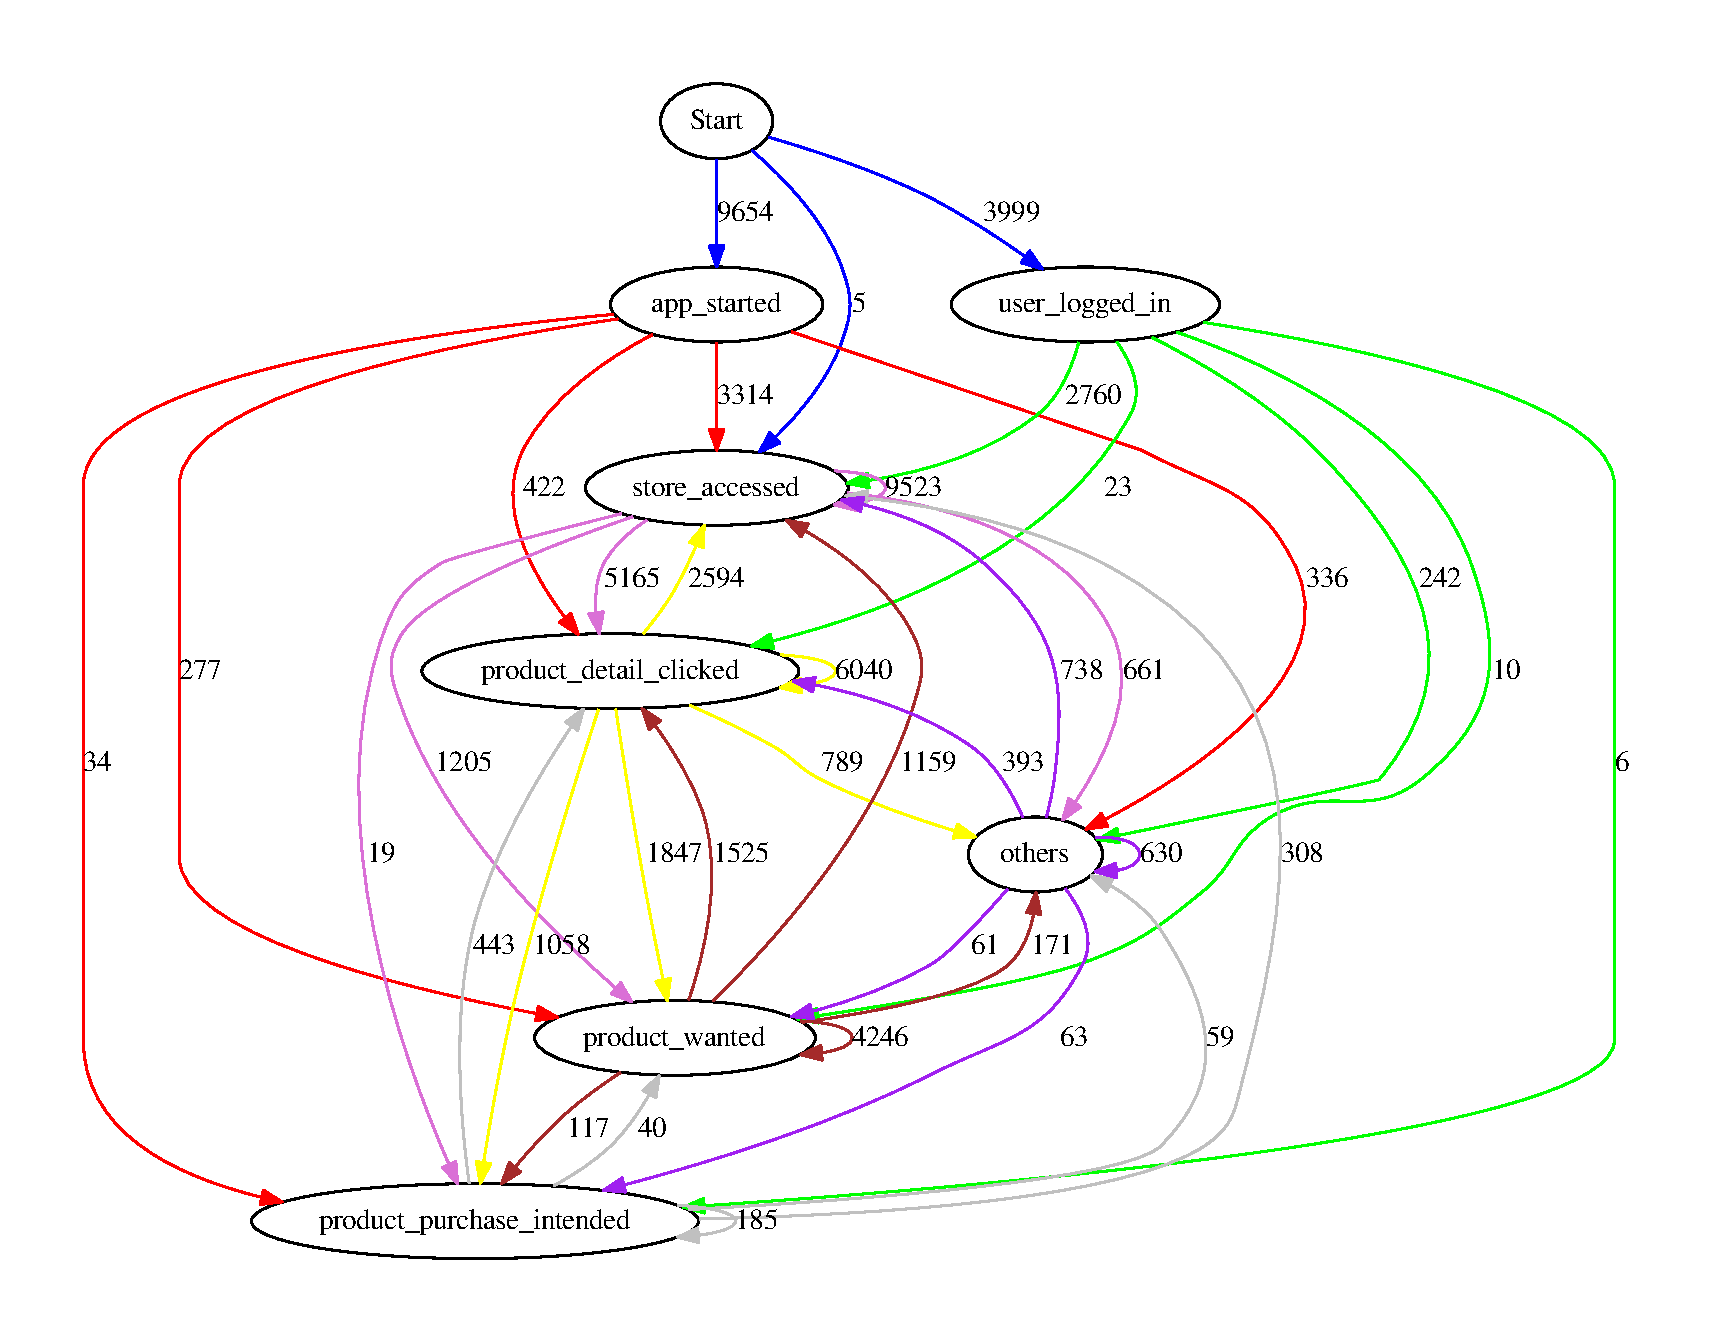
\includegraphics[width=5in]{image/statesInteractionTrue-gvfile.pdf}
        \centering
        \caption{A minimized view of the different states of the system and how they interact with each other.}
        \label{figure:minStatesInteractions}
    \end{figure}
        The figure above presents the events as states and shows the interactions between them.
        The weights on the edges between the states are the count of state changes from the sending state to the receiving state.
        As we can see from the figure, states can access themselves.
        This figure is a minimized view to better present the state interactions regarding products, where states such as \emph{activity\_clicked}, \emph{around\_me\_clicked} and \emph{stores\_map\_clicked}, have been left out to give focus to item interaction related states.
        For a more complete view without reduced states see~\ref{figure:statesInteractions}.

        The \emph{Init}-state is the initialization of the application, which leads to the \emph{Start}-state, which is a reduction of the variations of events which indicates that a session is started, such as \emph{user\_logged\_in}, \emph{app\_started} and \emph{app\_first\_started}.
        From this most of the users enter the \emph{store\_accessed}-state, which is the shared state of all the store related states.
        As we can see from the figure, in 12 477 cases the users enters a store after already having entered a store, which means that the user did not access any of the items in the first entered store, and we see that this is a common way of browsing the products in the application. Since this leaves little indication about the user preferences, other ways of gathering this must be utilized.
        While this thesis was being written additional events was added, one of these was \emph{content:interact:item\_scroll}, which has proven to be of good help to derive user preferences~\cite{Claypool01inferringuser}.

        If we focus on the states \emph{product\_wanted} and \emph{product\_purchase\_intended}, we see that 160 occurrences of being in the \emph{product\_wanted}-state progressed into the \emph{product\_purchase\_intended}-state.

%     Init Hypothesis:

%     Must make different rules for the different stores:
%     "Bik Bok", "Cubus", "Gina Trik", "H\&M", "Bianco" has a broad specter of extra
%     functions inside the web store, whereas others might not, only shows the
%     product and a add to chart button.  This might divide the use pattern of the
%     users into a:

%     "product\_detail\_clicked" $\Rightarrow$ "product\_purchase\_intended" $\Rightarrow$ "product\_wanted"

%     "product\_detail\_clicked" $\Rightarrow$ "product\_purchase\_intended" $\notimplies$ "product\_wanted",

%     and

%     "product\_detail\_clicked" $\Rightarrow$ "product\_wanted"

%     based on the store accessed.

%     Use this to make a "rule set" with a probability.
%     Then again use this to recommend items for the users with that given
%     probability.

%     Find a "most popular session"-pattern
%     Find a "most likely to come after"-pattern

\section{Conclusion}
\label{sec:dataset-conclusion}

%Summarize the findings
%What can be used?


% !TEX root = ../report.tex

\chapter{State Of The Art}
\minitoc
\label{chap:SotA}

This section will present and discuss previous work in the field of recommender
systems. First out is recommender system fundamentals which cover the main recommender
system techniques which the techniques described later in the chapter are based.
Next up is a round up of some existing solutions to the cold start problem, followed
by fashion recommender systems, session based approaches and lastly a summary
of how recommender systems can be evaluated.

\clearpage

% !TEX root = ../../report.tex

\section{Recommender Systems foundations}
\label{sec:recsys}
Recommender systems have become an important research topic since the
introduction of Tapestry \cite{Goldberg1992}, the first collaborative filtering
system back in 1992. Recommender systems now play an important role in many of
the most popular web-sites such as Amazon, YouTube, Netflix, TripAdvisor,
Last.fm, and IMDb. In its most common formulation the recommendation problem is
reduced to the problem of estimating the preference/rating of items that have
not been seen by a user. Usually, this estimation is based on one or more of
the following assumptions:

\begin{itemize}
\item You are like your friends
\item You are like people who do similar things that you do
\item You like things that are similar to things you already like
\item You are influenced by experts and the opinions of others.
\end{itemize}

Once we have estimated these ratings we can recommend the items with the
highest rating to the user. These recommendations relate to various
decision-making processes, such as what items to buy, what music to listen to,
or what online news to read. Recommender systems are usually classified into
the following categories, based on how the recommendations are made
\cite{Adomavicius2005}.

\begin{itemize}
\item \emph{Content-based recommendations:} The user will be recommended items with similar content to the ones the user preferred in the past;
\item \emph{Collaborative recommendations:} The user will be recommended items that people with similar testes and preferences have liked in the past;
\item \emph{Hybrid approaches:} These methods combine collaborative and content-based methods.
\end{itemize}

\subsection{Content Based Filtering}

In a content-based system, we must construct a user \emph{profile}
$ContentBasedProfile(c)$ or each user $c$, which is a record or collection of
the attributes which characterizes each item $Content(s)$ of all the items
$s_{i} \epsilon S$ previously rated by user $c$. For example in a fashion
recommender system the content-based recommender system tries to understand the
commonalities among the items user $c$ has rated highly in the past (color,
brand, store, price, etc.). Then recommend items that have a high degree of
similarity to these items. $ContentBasedProfile(c)$ can be designed as a vector
of weights $(w_{c1} ... w_{ck})$, where each weight $w_{ci}$ denotes the
importance of the keyword $k_{i}$ to user $c$.

Items that can be recommended to the user can often be stored in a database
table. Figure \ref{figure:contentbaseddb} shows a simple database with rows
describing 5 items that have been rated by 3 users. The column names starting
with $X_{n}$ are the properties of the items, often referred to as
"attributes".

\begin{figure}[H]
    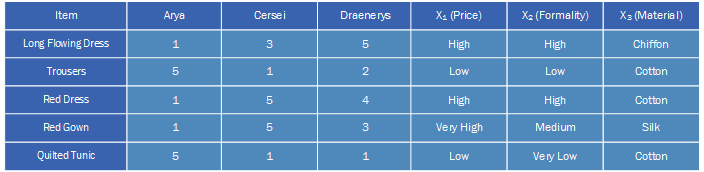
\includegraphics[width=5in]{image/contentbaseddb.png}
    \centering
    \caption[A clothing database]{A clothing database. Rows are items, columns are users and item attributes}
    \label{figure:contentbaseddb}
\end{figure}

From the rating matrix and content properties one can then construct a
$ContentBasedProfile(c)$ for each user $c$, for the user Arya one could imagine
it would look something like this.

\begin{figure}[H]
    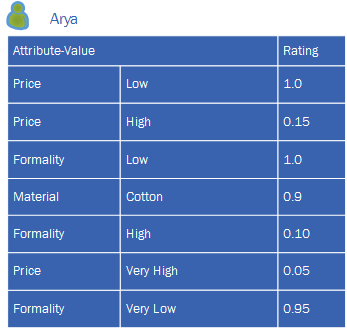
\includegraphics[width=2in]{image/contentprofile.png}
    \centering
    \caption[Content Profile Example]{Content Profile Example}
    \label{figure:contentprofile}
\end{figure}

The recommendation process consists of matching up the attributes of the user
profile against the attributes of an item. The result is a relevance judgment
that represents the user's level of interest in that object. The utility $u(c,
s)$ of item $s$ for user $c$ is estimated based on the utilities $u(c, s_{i})$
assigned by user c to items $s_{i} \epsilon S$ that exhibit a similarity to
item $s$. E.g. for the user Arya items with the attributes low price and low
formality could safely be recommended as they fit her user profile, and have
similar characteristics to the items which she previously have rated highly.
The utility function $r(u, i)$ is usually defined as:

\begin{equation}
r(u,i) = score(ContentBasedProfile(u), Content(i)).
\end{equation}

\subsection{Collaborative Filtering}
\label{subsec:cf}

The goal of collaborative filtering methods is to suggest new items or to
predict the utility $u(c, s)$ of a certain item s for a particular user c based
on the user's previous activities and/or likings and similarity to other users.
In a typical CF scenario, there is a list of $n$ users $C = {c_{1}, ... c_{n}}$
and a list of $m$ items $S = {s_{1},...s_{m}}$. Each user $c_{i}$ has a list of
items $S_{si}$, which the user have expressed her opinion about, which makes up
our rating matrix of size $S \times C$. More formally, the utility $u(c, s)$ of
item $s$ for user $c$ is estimated based on the utilities $u(c_{j}, s)$
assigned to item $s$ by the users $c_{j} \epsilon C$, which can be considered
"similar" to the active user $c$. This is exemplified in Figure
\ref{figure:ratingmatrix}. For example, in our fashion recommender system, in
order to recommend clothes to user $c$, the collaborative filtering method must
find the "peers" of users $c$, which share the same tastes in clothes (user
which tend to enjoy similar clothes). Then, recommend the clothes that are most
liked among these "peers".

\begin{figure}[H]
    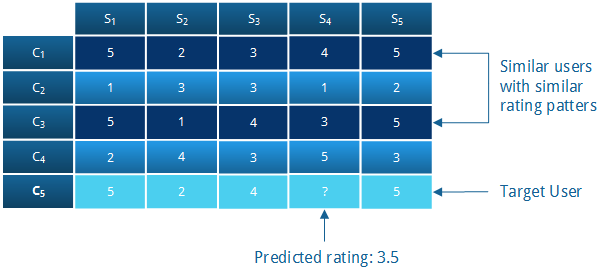
\includegraphics[width=5in]{image/ratingmatrix.png}
    \centering
    \caption[Collaborative filtering rating matrix]{Collaborative filtering rating matrix}
    \label{figure:ratingmatrix}
\end{figure}

Researchers have devised a number of collaborative filtering algorithms that
can be divided into two main categories: Memory-based and Model-based
algorithms \cite{Su2009}.\linebreak[4]

\begin{figure}[H]
    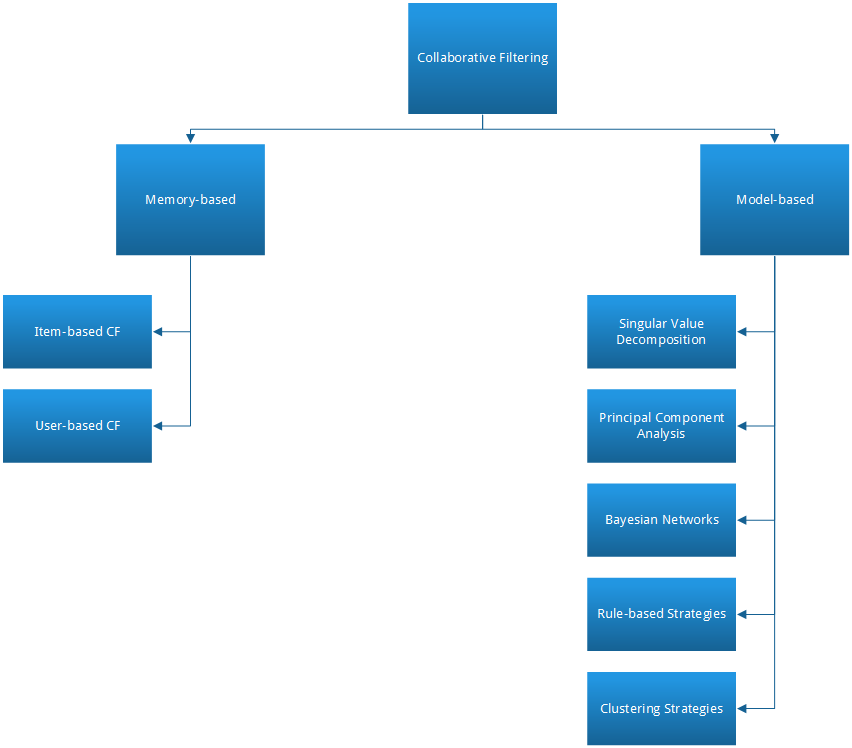
\includegraphics[width=5in]{image/cftaxonomy.png}
    \centering
    \caption[Classification of collaborative filtering techniques]{Classification of collaborative filtering techniques}
    \label{figure:cftaxonomy}
\end{figure}

\subsubsection{Memory-based Methods}

Memory-based Collaborative Filtering methods utilize the entire user-item
database to generate predictions. More formally, the value of an unknown
utility $u(c,s)$ for user $c$ and item $s$ is usually computed by taking the
weighted average of the utilities assigned by the $N$ most similar users for
the same item $s$. The similarity between user $c$ and $c'$, $sim(c, c')$ is
used as the weight. The more similar a user $c'$ is to $c$, the more weight is
given to the utility $u(c', s)$, and thus, will carry more weight in the
prediction for $u(c,s)$.

\begin{equation}
\label{equation:cfratingprediction}
u(c,s) = k * \sum_{c' \epsilon C} sim(c, c') * u(c',s)
\end{equation}

Where k serves as a normalization factor, usually being $1/|C|$. Various
approaches have been used to compute the similarity $sim(c, c')$ between the
users. Generally these approaches are based on the rating similarities for
items both users have rated. The most popular similarity measure is The Pearson
Correlation Coefficient. Equation \ref{equation:pearson} shows how to calculate
the Pearson Correlation Coefficient between two users $c$ and $c'$, Here
$S_{cc'}$ is the set of items both users have in \emph{common}.

\begin{equation}
sim(c, c') = \frac{\sum_{s \epsilon S_{cc'}} (u(c, s)-\bar{u_{c}})(u(c',s)-\bar{u_{c'}})}{\sqrt[•]{\sum_{s \epsilon S_{cc'}} (u(c, s)-\bar{u_{c}})^{2}(u(c',s)-\bar{u_{c'}})^{2}}}
\label{equation:pearson}
\end{equation}

Where $u_{c}$ is the mean utility of user $c$. The Pearson Correlation
Coefficient and other similarity measures such as consine based approaches are
more commonly known user-based collaborative filtering.\newline

Item-based Top-N Recommendation methods calculates the similarity between items
instead of users. In these approaches, the historical information is analyzed
to identify the relations between items such that a purchase of another item
(or set of items) often leads to the purchase of another item. These models are
often used since they quickly can recommend a set of items, and have shown to
produce recommendation results comparable or better than traditional user-based
approaches \cite{Karypis2001}.

The algorithm first computes the $k$ most similar items for each item according
to the ratings given by users they both share. Once the most similar items are
found, the prediction is then computed by taking the weighted average of the
target user's ratings on these similar items.

\begin{equation}
u(c,s) = \frac{\sum_{all similar items, S} (sim(s,S)u(c, S)}{\sum_{all similar items, S}(|s,S|)}
\end{equation}

Items that often are rated similarly by users are considered more similar than
items which share few similar ratings. Figure \ref{figure:itemsim} illustrates
the process of finding the item-similarities.

\begin{figure}[H]
    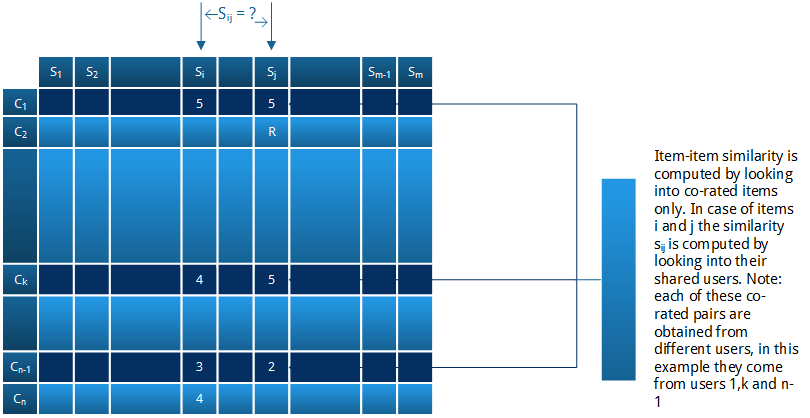
\includegraphics[width=5in]{image/itemsim.png}
    \centering
    \caption[Item-item similarity]{Item-item similarity}
    \label{figure:itemsim}
\end{figure}

There are a number of ways of computing the similarity between items. E.g. by
means of cosine-based similarity. In this case, two items are though of as two
vectors in an $C$ dimensional user space. The similarity between the items is
found by computing the cosine of the angle between the two vectors.

\begin{equation}
sim(s',s) = cos(\vec{s'},\vec{s}) = \frac{\vec{s'} \cdot \vec{s}}{\|\vec{s'}\|^{2} * \|\vec{s}\|^{2}}
\end{equation}

The item similarities can then used to find the Top-N recommendations. Each
user has a set of items $S_{c}$ previously rated by the user which we want to
compute top-N recommendations for. First, we identify the set $C$ of candidate
items recommended items by taking the union of the $k$ most similar items and
removing each of the items in the set $S_{c}$ the user already has rated; then
calculate the similarities between each item of the set $C$ and the set
$S_{c}$, using only the $k$ most similar items for each item in $S_{c}$. The
resulting set of items in $C$ are sorted in descending order of similarity and
will be the recommended as the item-based Top-N list \cite{Karypis2001}.

\subsubsection{Model-based Methods}


As the name implies, Model-based approaches provide recommendations by first
developing a model of the user ratings, which is then used to make predictions.
These algorithms develop a model of user ratings rather than identify a
neighborhood of similar users or items. These models can be built using various
strategies, such as Singular Value Decomposition (SVD), Principal Component
Analysis (PCA), Rule-based Strategies, Clustering Strategies and Bayesian
Networks.

Latent factor models is probably the most representative approach. Latent
factor models transform both items and users to a latent factor space. The
latent factor space tries to explain the ratings by characterizing both items
and users on factors automatically inferred from the data. The most popular
latent factor models are based on matrix factorization techniques
\cite{Koren2009}.

The main idea behind matrix factorization is just as its name implies,
factorize a matrix, finding two or more matrices such that when you multiply
them you get back the original matrix. Matrix factorization can be used to
discover latent factors underlying the interactions between the users and
items. These factors \emph{explain} how a user rates an item (i.e. that a user
would give high ratings to a certain shirt if he likes the brand, or if the
color is nice). If we can discover these factors, we should be able to predict
a rating with respect to a certain user and a certain item based on the
correlation between their factors.

A matrix factorization model map both users and items to a joint latent factor
space of dimensionality $f$, where $f$ is the number of latent factors. The
number of latent factors are usually determined by using a hold-out dataset or
cross-validation by evaluating the prediction error experimenting with
different values. It is also worth mentioning that this in some ways can be
seen as a trade-off between model building complexity and accuracy as having
more features makes the model building more expensive. Each user $c$ is
associated with a vector $p_{c} \epsilon \mathbb{R}^{f}$, and each item $s$ is
associated with a vector $q_{s} \epsilon \mathbb{R}^{f}$. Giving us a matrix Q
containing the user factors and a matrix P containing the item factors as
exemplified in Figure \ref{figure:matrixdecomp}.

\begin{figure}[H]
    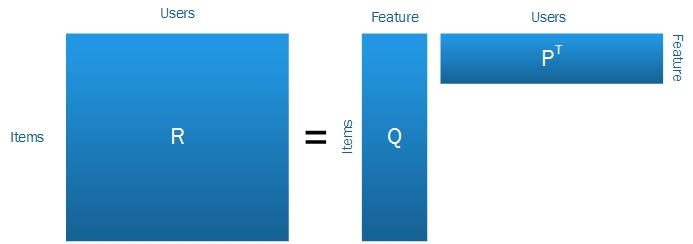
\includegraphics[width=5in]{image/matrixdecomp.jpg}
    \centering
    \caption[Matrix decomposition of the rating matrix $R$]{Matrix decomposition of the rating matrix $R$}
    \label{figure:matrixdecomp}
\end{figure}

User-item interactions are modeled as inner products in that space. For a given
item $s$, the elements of $q_{s}$ measures the extent to which the item
possesses those factors, positive or negative. Likewise, for a given user $c$,
the element $p_{c}$ measures the extent of interest that user has in items that
are high on the corresponding factors. The resulting dot product $\hat{u(c,s)}$
captures the overall interest of the user in the characteristics of the items.

\begin{equation}
u(c,s) = p_{c}^{T}q_{s} = \sum_{k=1}^{f} q_{sk}p_{kc}
\end{equation}

The problem then, is to discover the user factor matrix $P$ and the item factor
matrix $Q$ such that their product approximates the original rating matrix $R$.

\begin{equation}
R \approx Q \times P^{T} = \hat{R}
\label{equation:dotproduct}
\end{equation}

To learn the factor vectors the system minimizes the regularized square error
on the set of known rating $K$.

\begin{equation}
\label{equation:minimize}
min_{q, p} = \sum_{(c,s)\epsilon K} (u(c,s) - p^{T}_{c}q_{s})^{2} + \lambda ( \Vert q_{s} \Vert ^{2} + \Vert p_{c} \Vert ^{2})
\end{equation}

However, it is important to remember that our goal is generalize beyond the
observed ratings, in a way that we can predict future unknown ratings. The
system should therefore avoid overfitting the data by regularizing the learned
parameters, whose magnitudes are penalized. $\lambda$ controls the extent of
regularization, and much like $f$, often determined by cross-validation. Two
possible approaches to minimizing Equation \ref{equation:minimize} is to use
Stochastic Gradient Descent or Alternating Least Squares \citep{Koren2009}.\newline

Consider the following example where we have the following rating matrix R
shown in Table \ref{table:ratingMatrix} containing the rating of four users $C$
for four items $S$, giving us a $C \times S$ matrix with explicit ratings on a
  scale from 1 to 5.

\begin{table}[!htbp]
    \centering
    \begin{tabular}{|c|c|c|c|}
    \hline
    5.00    & 5.00  & 2.00 & -    \\ \hline
    2.00    & -     & 3.00 & 5.00 \\ \hline
     -      & 5.00  & -    & 3.00 \\ \hline
    3.00    & -     & -    & 5.00 \\ \hline
    \end{tabular}
    \caption{Rating matrix R ($C \times S$)}
    \label{table:ratingMatrix}
\end{table}

Given that $f = 3$, we might end up with the following matrix $P$ and $Q$

\begin{table}[!htbp]
\centering
\begin{tabular}{|c|c|c|}
\hline
1.81    &1.62   &0.74\\ \hline
2.66    &1.71   &-1.08\\ \hline
1.73    &-0.23  &0.78\\ \hline
3.16    &-0.24  &0.90\\ \hline
\end{tabular}
\label{table:ItemFeature}
\caption{User factor matrix $P$ ($C \times f$)}
\end{table}

\begin{table}[!htbp]
\centering
\begin{tabular}{|c|c|c|c|}
\hline
1.12    &   1.49    &   0.48\\ \hline
1.31    &-0.52  &0.59\\ \hline
1.13    &0.67&  -0.52\\ \hline
1.39    &0.05&  0.45\\ \hline
\end{tabular}
\label{table:UserFeature}
\caption{Item factor matrix $Q$ ($S \times f$)}
\end{table}

Equation \ref{equation:dotproduct} then gives us the following rating prediction matrix $\hat{R}$.

\begin{table}[!htbp]
\centering
\begin{tabular}{|c|c|c|c|}
\hline
4.79    &5.01   &1.97   &3.61 \\ \hline
1.97    &1.96   &2.85   &4.80 \\ \hline
2.75    &4.71   &1.40   &2.94 \\ \hline
2.93    &3.30   &2.74   &4.78 \\ \hline
\end{tabular}
\label{table:PredictionMatrix}
\caption{Rating prediction matrix $\hat{R}$}
\end{table}

As you can see the values of known ratings in Table \ref{table:ratingMatrix}
are fairly similar to the corresponding ratings in the rating prediction
matrix.

\subsection{Hybrid approaches}

A term \emph{hybrid recommender systems} is used to describe any recommender
system that combines multiple recommendation techniques together to provide
recommendations. Burke et al. \cite{Burke2002} identified seven different
classes of hybrid recommender systems:

\begin{itemize}
\item Weighted: The score of different recommendation components are combined numerically.
\item Switching: Switching between recommender systems depending on the situation.
\item Mixed: Recommendations from different recommenders are presented together.
\item Feature Combination. Features derived from different knowledge sources
are combined together and given to a single recommendation algorithm
\item Feature Augmentation: One recommendation technique is used to compute a
feature or set of features, which is then part of the input to the next
technique.
\item Cascade: Recommenders are given strict priority, with the lower priority
ones breaking ties in the score of the higher ones
\item Meta-level: One recommendation technique is applied and produces some
sort of model, which is then the input by the next technique
\end{itemize}

Most commonly hybrid systems are built by combining collaborative and
content-based methods in an attempt to mitigate the limitations the approaches
suffer individually. Adomavicius and Tuzhilin \cite{Adomavicius2005} lists the
following approaches to building hybrid recommender systems:

\begin{itemize}
\item Implementing the systems separately and combining their predictions
\item Incorporating content-based characteristics into a collaborative approach
\item Incorporating collaborative characteristics into a content-based approach
\item Constructing a general unifying model that incorporates both
content-based and collaborative characteristics
\end{itemize}

\subsection{Recommender System Challenges}

Below we briefly mention some of the main challenges one faces when working
with recommender systems.

\subsubsection{Scalability}

As the number of existing users and items blow up, traditional CF algorithms
suffer serious scalability problems. The model building phase of \emph{Traditional}
collaborative filtering methods have a complexity of O(MN) where $M$ is the number
of users and $N$ is the number of items. For systems with millions of users and items,
even a complexity of $n$ is too large. Another fundamental issue is how to embed the
core recommendation techniques in real operational systems and how to deal with massive
and dynamic sets of data produced by the interactions of users with items. Recommender
systems are expected in many cases to provide rapid recommendations online, it is
therefore also important to consider how fast the system provides recommendations.

Better scalability and improved accuracy make the item-item collaborative filtering
approaches more favourable in many cases. The computational complexity of item-to-item
based algorithms are up to two orders of magnitude faster than traditional user-based
algorithms \cite{Deshpande2004}. Dimensionality reduction techniques such as
SVD can deal with the scalability by providing more compact representations and
quickly produce good recommendations. However, most dimensionality reduction
techniques must undergo expensive matrix factorization steps.

\subsubsection{Sparsity}

In practice, many recommender systems deal with very large item collections.
This means that the number of ratings obtained is usually very small compared to the
number of ratings that it needs to predict. Efficient prediction of ratings from a small
number of examples is therefore important. The \emph{reduced coverage} problem
occurs when the number of users' rating may be very small compared to the number of items.
This may lead to that the recommender is unable to provide recommendations for a large
portion of the items. \emph{Neighbour transitivity} refers to the problem in which users
with similar tastes may not be identified due to a lack of co-rated items, making
collaborative filtering futile, since it relies on comparing users to predict unknown ratings.

\subsubsection{Cold-start}

Conceptually, the cold-start problem can be viewed as a special instance of the
sparsity problem, where most elements in a certain row or column are zero. The
cold-start problem further emphasizes the importance of the sparsity problem.
Whenever a new user or item enters the system, it is difficult to find similar
ones as there is little or no information available. New items can therefore
not be recommended until they have been recommended by a substantial amount of
users. Similarly, giving \emph{good} personalized recommendations to new users
based on a few ratings is difficult, since it does not give a good overall
picture of a users tastes and preferences. These problems are known as the
\emph{cold-start user} and \emph{cold-start item} problems.

\subsubsection{Shilling attacks}

In recommender systems where everyone can give ratings, people may give lots of
positive ratings to their own items and negative ratings to their competitors.
It is often necessary for collaborative filtering systems to introduce
precautions to discourage such kind of manipulation.

\subsection{Terminology}

%TODO - Any more RS related terminology that needs explaining?

\subsubsection{Explanations / Transparency}

Tintarev et al. \cite{Tintarev2007} lists seven roles a that can be played by explanations in recommender systems:

\begin{itemize}
\item Transparency: Explaining how the system works
\item Scrutability: Allowing the users to tell the system it is wrong
\item Trust: Increasing user confidence in the system
\item Effectiveness: Help users make good decisions
\item Persuasiveness: Convince users to try or buy
\item Efficiency: Helping users to make decisions faster
\item Satisfaction: Increasing the ease of use or enjoyment
\end{itemize}

In collaborative filtering systems the explanations is of the form "Other users
similar to you liked this item", while in content-based style explanations, the
item's attributes which most affected the item to be recommended to the user
are illustrated. For example, in a fashion recommender, an explanation may be
of the form "This shirt was recommended because it's a Ralph Lauren who you
seem to like".

% !TEX root = ../../report.tex
\section{The Cold-start Problem}

%Can the different approaches be classified? E.g. 3 main categories of approaches
    %Initial categorization
        %Interview process
        %Hybrid approaches
        %Key figures / Seed users
        %Filterbots
        %Trust-aware / Trust propagation

In the literature, the term cold is used about an object in a system, or a
whole system, which is new \cite{Schein2002, Park2006}. Cold-start scenarios in recommender systems are
situations in which little/no prior events, like ratings or clicks, are known
for certain users or items. The cold-start problem can be divided into three sub problems:

\begin{itemize}
  \item \emph{Cold-start system}: A situation where we only have new users and
  little or no ratings for the items.

  \item \emph{Cold-start item}: The problem of recommending items that are new
  to the system, which have not received any ratings.

  \item \emph{Cold-start user}: The problem of giving accurate recommendations
  to a user who is new to a recommender system.
\end{itemize}


For example in a scenario where the average item in an item collection have 5
000 ratings, a new item with only 5 ratings would be considered a
\emph{cold-item}. Likewise, in a recommender system where the average user has
rated 25 items, a user who only has rated 2 items, would be considered a
\emph{cold-user}.

The cold-start system problem is mainly a collaborative filtering problem, and
can be seen as a combination of the cold-start user and cold-start item problem
where the majority of the users are new to the system and have expressed few
preferences, resulting in a very sparse user-item matrix, rendering traditional
collaborative-filtering methods futile. Most traditional algorithms only work
effectively in environments where the datasets has high information density. In
fact, in extreme cases, when data is very scarce, simple non-personalized
recommendations based on global averages can outperform collaborative-filtering
algorithms \cite{Park2006}. The reason why the cold-start system problem is not
so evident in content-based systems is due to \emph{User Independence}, meaning
that the system only exploits ratings provided by the active user to build her
profile. Instead, collaborative filtering methods need ratings from other users
to find the "peers" of the active users.

In content-based systems, new items can easily be recommended using the content
information of the item, making it a popular solution to the \emph{cold-start
item} problem. This problem is more severe in collaborative-filtering systems
where items are only recommendable if they have been rated by substantial
amount of users. New items will therefore not be recommendable before multiple
users somehow stumble upon the new item while e.g. browsing the item
collection, unless additional measures are taken to solve this problem. To
\emph{solve} the new-item problem, there are two commonly used (simple)
solutions often used in E-commerce websites:\marginpar{heri-notes: cite}

\begin{itemize}

\item Advertising at the front-page of the website, putting the new items in an
eye catching position. This solution, however, may this result in that some
users, which don't like these new items, might leave the website.
\item Requesting the user to choose one or more of his/hers categories while
registering for the site, and recommend items from the selected categories.
This approach however, requires active user involvement and complicates the
sign up process. Many users might chose not to give up any personal interest
information, thus the user group covered by this solution could end up not
being large enough.
\end{itemize}

The cold-start user problem is present both in content-based and collaborative-filtering systems.
Since Collaborative Filtering is based on the idea that like-minded users have similar tastes and
preferences, a new user therefore naturally poses a challenge to a CF recommender, since the system has no knowledge about
the preferences of the new user, and can therefore not find any like-minded users. The system must therefore acquire some
information about the new user before it can start making personalized recommendations. In a typical domain, for example
in the domain of books, the number of items is very large (in the order of tens of thousands) while the number of items
rated by every single user is in general small (in the order of dozens or less). This means that it is very unlikely two
random selected users have rated any items in common and hence they are not comparable. The system will therefore most
likely struggle to find users with tastes that are \emph{truly} similar to the target user. Similarly, in content-based
systems, the lack of ratings given by the target user, means that the target user will have a limited content-profile,
since the users content profile is constructed using content-information from his/hers rated items. In both cases,
recommendation quality is most likely bound to suffer.\newline

\marginpar{heri-notes: hvordan kan dette problemet være relevant for oppgaven deres?}

This section will present a few different solutions to the cold-start problem, focusing mainly on \emph{complete} solutions to the cold-start problem.

\subsection{Trust Aware Recommender Systems}

One promising direction to solve the cold-start problem is the incorporation of
a trust network. A trust network can significantly help alleviate the
cold-start user problem, primarily since the trust statements between users can
be propagated and aggregated, and consequently connect more people and
products. By making clever connections in the trust network, newcomers can
immediately gain access to a wide range of connections.

%Due to the popularity of social networks such as Facebook, more and more
%researchers turn to incorporate the social relationships (e.g. trust) of users
%to help complement users’ preference in addition to item ratings, in order to overcome the limitations of existing recommender systems

For example, when looking for movie recommendations we often turn to our friends which we share a similar taste in movies with. Trust can be defined as: "believe in the reliability, truth, or ability of", and in the context of recommender systems a trusted user would be a user you trust to provide you with good recommendations. E.g. in the case of the Epinions dataset \cite{Epinions}, users can explicitly state whether they trust or distrust a user [1, -1], i.e. reviewers whose reviews and ratings they have consistently found to be valuable or reviewers which they find consistently offensive, inaccurate or not valuable. In decentralized environments where everyone is free to create content and there
is no centralized quality control entity, evaluating the quality of the content becomes an important issue. This phenomenon can be observed in online
marketplaces such as E-bay where users can create "fake" auctions and in peer-to-peer networks where peers can enter corrupted items. In these environments, it is often a good strategy to delegate the quality assessment task to users themselves. E.g. \emph{Ebay.com} allows users to express their level of satisfaction after every interaction with another user. Trust relationships of users are often employed in order to correlate more potential raters for the active users who require recommendations \cite{Massa2004, Massa2007}. Massa et. al. \cite{Massa2004} also show that some of the weaknesses of recommender systems such as data sparseness and their susceptibility to shilling attacks could be alleviated by incorporating trust.

% The formals
In \cite{Massa2004}, Massa et al. proposes a Trust-Aware recommender system
architecture.  To capture all the trust statements we need a $CxC$ matrix,
where $C$ is the number of users, since each user is allowed to express a trust
value in every other user. This matrix will make up our trust network among the
users. If $u$ trusts $v$, then there is a value $t_{u,v}$ for this trust which
is a real number in $[0,1]$. Zero means no trust and one means full trust. This
additional information can be organized in a trust network and a \emph{trust
metric} can be used to predict the trustworthiness of other users as well (for
example, friends of friends). The idea here is to not search for similar users
as CF does but to search for trust-able users by exploiting trust propagation
over the trust network. The items appreciated by these users are then
recommended to the active user.

% Web of Trust - Figure explanation
Consider the example shown in Figure \ref{figure:weboftrust}. User $A$ has
issued a trust statement in $B$ and $C$; hence $B$ and $C$ are in the web of
trust of $A$. Using these explicit trust statements, it is possible to predict
trust in unknown users by propagating trust, making it possible to infer
something about how much user $A$ could trust $D$.

\begin{figure}[H]
    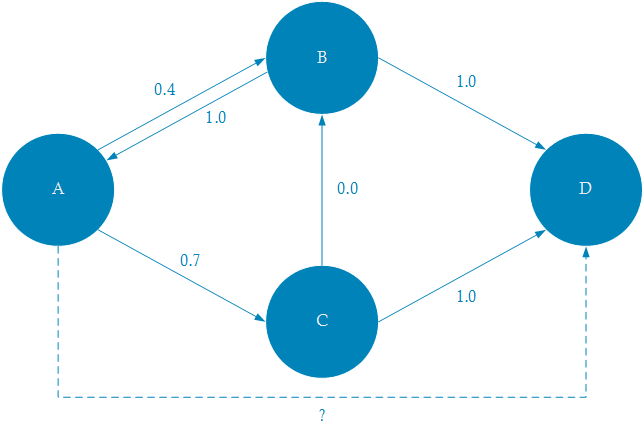
\includegraphics[width=2in]{image/webofTrust.png}
    \centering
    \caption[Trust Network]{Trust Network. Nodes are users and solid edges are trust statements. The dotted edge is one of the undefined and predictable trust statements (Adopted from \cite{Massa2004})}
    \label{figure:weboftrust}
\end{figure}

In addition to the trust network we will also have a rating matrix of size
$CxS$, where $S$ is the number of items. This rating will not differ from a
standard rating matrix, which are used in traditional collaborative filtering
systems. The value $u(c,s)$, is the rating given by user $c$ to item $s$, the
rating scale may differ from system to system.

% Architecture
The systems takes as input the trust network and the ratings matrix and
produces, as output, a matrix of predicted ratings that the users would assign
to the items. Figure \ref{figure:trustarchictecture} shows a conceptual
overview of the trust-aware recommender system architecture.

\begin{figure}[H]
    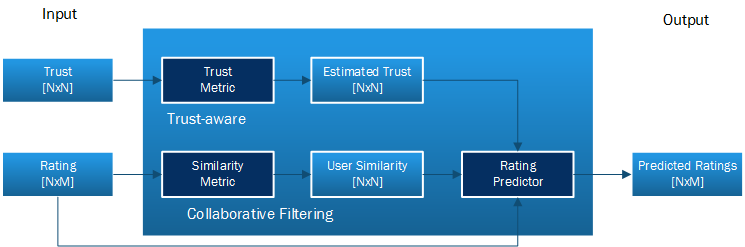
\includegraphics[width=5in]{image/trustawarearchitecture.png}
    \centering
    \caption[Trust-Aware Recommender System Architecture]{Trust-Aware
    Recommender System Architecture (Adopted from \cite{Massa2004})}
    \label{figure:trustarchictecture}
\end{figure}

The \emph{Trust Metric} module takes the trust network as input, and exploits
trust propagation in order to predict, for every user, how much she could trust
other users. Trust metrics can either be local and global. Global trust metrics
produces an estimated trust matrix with all the rows equal, meaning that the
estimated trust in a certain user (column) is the same for every user (row). A
simple local trust metric could e.g. for each user assign to every other user a
predicted trust based on her minimum distance from the source user. More
sophisticated ones could also be employed. If we again consider Figure
\ref{figure:weboftrust}, we could employ a local trust metric where the
predicted trust is based on the minimum distance from the source user. If we
set the maximum propagation distance $d$, a user at distance $n$ from the
source user will have a predicted trust value of:

\begin{equation}
t_{u,v} = \frac{d-n+1}{d}
\end{equation}

Giving users not reachable within the maximum propagation distance a trust of
$0$. Using user $A$ as the source user, the users at distance $1$ ($B$ and $C$)
would get a trust value of $(4-1+1)/4 = 1$, while the user at distance 2 (D)
would get a predicted trust value of $(4-2+1)/4 = 0.75$. Meaning that we will
have a linear decay in trust based on the distance from the source user.

Massa et al. \cite{Massa2007} experimented with both local and global trust
metrics. They used the PageRank algorithm as a global trust metric. PageRank
tries to infer the authority of every single user by examining the structure of
the network. The algorithm follows a simple idea: if a link from user $A$ to
user $B$ represent a positive vote casted by $A$ to $B$, then the global rank
of a page depends on the number (and quality) of the incoming links. The trust
values assigned by users to users are used to predict the trustworthiness of
unknown users. Their findings, not surprisingly, indicate that Global Trust
Metrics are not suited for the task of finding good neighbours, especially for
providing personalized recommendations, but is more suited to applications such
as \emph{Ebay.com} to find untrustworthy users. As a local trust metric they
used MoleTrust, which is a depth-first graph walking algorithm with a tuneable
trust horizon which allowed them to experiment with different propagation
distances. They found trusted users to be good predictors. For the cold-start
users they achieved a MAE of 0.674 when looking at friends of friends, compared
to traditional collaborative filtering which scored 1.094. The difference is
very high, and particularly relevant as it is important for recommender systems
to generate personalized recommendations as soon as possible for new users, so
that these users appreciate the system and keep using it.

The \emph{Similarity Metric} module computes the user similarities, this is one
of the standard steps of any traditional collaborative filtering technique,
user similarities can be found e.g. by using the Pearson Correlation
Coefficient. The intuition is that, if a user rates in a similar way to another
user, then her ratings are using for predicting the ratings for that users.

The \emph{Rating Predictor} can use the neighbours from the user similarity
matrix, the estimated trust matrix or a combination of both in order to
calculate the predicted ratings.

% Using a Trust Network to Improve Top-N Recommendation

Jamali et al. \cite{Jamali2009} propose two different methods for getting
around the cold-start user problem using a trust network. Their first approach
called \emph{Random Walk} only utilize the trust network to provide
recommendations. Starting from the active user $u$, we perform a random walk on
the trust network. Each random walk stops at a certain user. Then the items
rated highly by that user will be considered as recommended items, ordered
according to the ratings expressed by that user. Several random walks are
performed to gather more information and compute a more confident result. The
estimated rating of each item is the average of ratings for that item over all
raters considered. At the end, we output items with the highest estimated
rating as top-N recommended items. Their second approach called \emph{Combined
Approach} uses both user-user similarities and the trust network to provide
recommendations. In this approach we compute the top $K$ trusted users in the
network and rank the items rated by these trusted users to compute top-N
recommended items. The top $K$ trusted users can either be found by
\emph{Breadth First Search} or \emph{Random Walk in the social network}. We use
the collaborative filtering approach to compute another set of top-N
recommended items. Finally, we merge these two lists to produce a combined list
of top-N recommended items. Items returned by CF is denoted as $CF_{u}$, while
the items returned by Trust-based approach are denoted $TR_{u}$.

\begin{equation}
 \hat{u}(c,s) =
  \begin{cases}
   \frac{u_{tr_{c,i}}+u_{cf_{c,i}}}{2}     & i \in TR_{u};i \in CF_{u}         \\
   \hat{u_{tr_{c,i}}}                      & i \in TR_{u};i \not \in CF_{u}    \\
   \hat{u_{cf_{c,i}}}                      & i \in CF_{u};i \not \in TR_{u}     \end{cases}
\end{equation}

The top-N items with the highest value of $\hat{u}(c,s)$ will be returned as
the top-N recommended items. The authors also experimented with weighted
averaging in the case where the item appear in both $TR_{u}$ and $CF_{u}$.

The top-N items with the highest value of $\hat{u}(c,s)$ will be returned as
the top-N recommended items. The authors also experimented with weighted
averaging in the case where the item appear in both $TR_{u}$ and $CF_{u}$.
Their approaches showed great improvements in recall for cold-start users,
improving the performance by 50\% over standard CF methods. The main
improvements however, are the coverage of the trust-based approaches, while
still maintaining the same or even slightly better precision than the standard
CF methods.

% Trust-aware Recommender Systems + Trust-Aware Collaborative Filtering for Recommender Systems
% Article Comments:
%   Requires user involvement (explicitly express trust) - is this a acceptable?

%Massa et al. \cite{Massa2004, Massa2007} propose using trust information
%explicitly expressed by the users. Users are allowed to state how much they
%consider every other user trustworthy that, in the context of recommender
%systems, is related to how much they consider the ratings provided by a certain
%user valuable and relevant.

% Alleviating the Sparsity Problem of Collaborative Filtering Using Trust Inferences
% Article Comments:
%   - Pretty good general model for dealing with sparsity
%   - Requires no additional information such as product details, demographic information about userstrus


Papagelis et al. \cite{Papagelis2005} proposed to alleviate sparsity using
trust inferred from user-user similarity. This approach does therefore not
require users to explicitly express their trust in other users, unlike the
approaches described above, the trust information is inferred from the
underlying social network of the rating matrix. Their approach is based on the
assumption that the more similar two users are, the greater their established
trust would be considered.

\begin{figure}[H]
    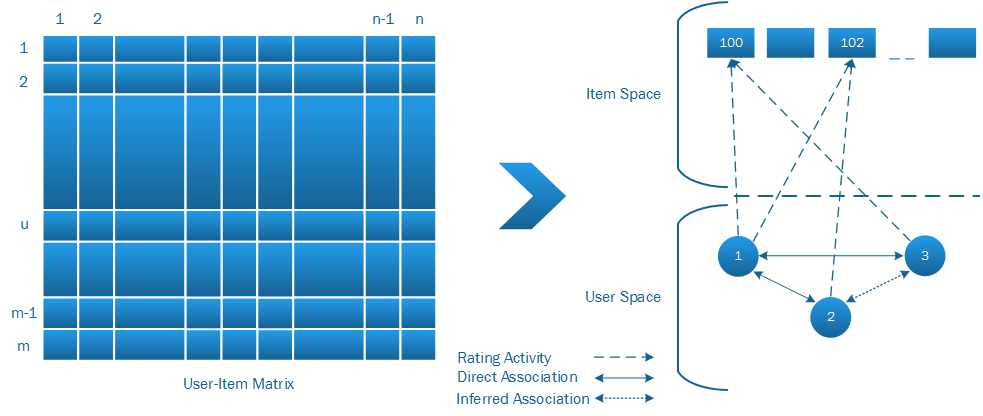
\includegraphics[width=5in]{image/trustnetwork.png}
    \centering
    \caption[Underlying Social Networks in Recommender Systems]{Underlying Social Networks in Recommender Systems}
    \label{figure:cfsocialnetwork}
\end{figure}

Due to the number of ratings that exist in recommendation systems, underlying
social networks are very sparse. There are cases in which insufficient or loss
of information is detrimental for the recommendation algorithms. Consider
Figure \ref{figure:cfsocialnetwork}, classic CF will associate only the users
which have co-rated an item (User $1$ and $2$ and user $1$ and $3$). To deal
with the problem of a sparse social network, it is possible to infer trust
between a source user $S$ and a target user $T$ through an intermediate user
$N$ (User $2$ and $3$ are connected through the intermediary user $1$), as
shown by the \emph{Inferred Association} arrow. According to this process,
trust is propagated in the network and associations between users are built,
even if they have no co-rated item. Trust paths can be of variable length,
depending on the number of associations that one needs to traverse in order to
reach the target user.

% Trust-paths
For example, if the trust $t_{(1,2)} = 0.7$ based on 5 co-rated items
and $t_{(1,3)} = 0.35$ based on 2 co-rated items, then the trust
between user $2$ and $3$ through $1$ is, $\frac{0.7*5}{5+2} + \frac{0.35*2}{7} = 0.6$.

In order to express the subjective notion of trust, the authors set up a
confidence model that is assigned to each direct association of the network
that expresses the reliability of the association. Confidence is related to the
number of co-rated items between two users. The confidence scores are all
expressed in relation to the most confident association for each user.

\begin{equation}
c_{(s,t)} = \frac{n(I_{s} \cap I_{t})}{n(I_{s} \cap I_{u_{MAX_CONF}})}
\end{equation}

Using the above example, assuming that the maximum number of co-rated items
user $1$ has with any user is 7, $c_{(1,2)} = \frac{5}{7}$.

% Results/Findings
The authors achieved improved accuracy for all sparsity levels. With a sparsity
level of $99.9\%$ the 2-HOP CF (friend of friends) increased the MAE
performance by $17\%$ over standard CF methods.

%TODO - READ: A Matrix Factorization Technique with Trust Propagation for Recommendation in Social Networks
%Jamali et al. propose a technique for incorporating trust using matrix factorization, called SocialMF.
%Leverage regularization model to fusing the one mode data by minimizing the gap between the taste of a user and the taste of her trusted friends
%In their model, the users which have not expressed any ratings feature vectors will be learned to be close to their trusted neighbors.

Victor et al. \cite{Victor2008} points out that cold-start users not only have
expressed few ratings, but also typically have expressed trust in few users. In
order for trust-aware recommenders to help cold-start users they need to have
expressed trust in atleast one user. But choosing who to connect to is often a
difficult task. To help cold-start users find trusted users, Victor et al.
propose using key figures or mavens (users who write many reviews), frequent
raters (users who evaluate many items) and connectors (users with
many trust connections). By connecting to these key figures, cold-start users
shown a significant increase in coverage while still maintaining good accuracy.
They also show that connecting to key figures are more beneficial to a
cold-start user than connecting to a random user.

\subsection{Filterbots}

% Na¨ıve Filterbots for Robust Cold-Start Recommendations

Park et al. \cite{Park2006} propose using filterbots to improve the cold-start
performance of collaborative filtering methods. Their filterbots are a varition
of RipperBots, described in detail in \cite{Good1999}. A filterbot is an
automated agent that rates all or most items using information filtering (IF)
techniques. The filterbots injects psuedo users or bots into the system. These
bots rate items algorithmically according to item features and user profiles.
For their movie recommendation systems the authors used 7 global bots which
e.g. rated movies based on average item rating, a critic bot that generates ratings
based on the average critic (pre-selected users) ratings, an award bot that
generates rating based on the awards a movie has won, and so on. These ratings
generated by these bots are injected into the user-item matrix along with
actual user-item ratings. Standard CF algorithms are then applied to generate
recommendations.

Their approach clearly demonstrated better robustness to all three cold-start situations than standard item-based
and user-based collaborative filtering. The improvements were most evident on
the datasets with a high degree of sparsity.

\subsection{Wisdom of the better few / Seed users}

% Wisdom of the Better Few: Cold Start Recommendation via Representative based Rating Elicitation

Liu et al. \cite{Liu2011} propose an approach in which they elect a few
representative users and items. The representative set should represent a set
of active users or items who well represent the entire population but with
little taste overlap. In their approach they wish to find a rank-k
factorization of the form $Y \approx XR$ or $Y \approx CX$ where $X$ is a
loading matrix consisting of free parameters and $R$ and $C$ which is the
component matrix consisting of actual rows or columns from $Y$. The
representative users and items are found using dimensionality reduction
techniques by reducing the column space of the rating matrix from $m$ to $k$.
And then applying basis selection based on the maximum-volume principle to
select the $k$ most representative users or items. In order to be able to
recommend new items to the users it must first be rated by the $k$
representative users, likewise for new users to be rated they need to rate the
$k$ most representative items. Their method therefore easily allows new users
and items to be \emph{folded in}.

\subsection{Intelligent Selection / Interview Process}\mbox{}\\

\begin{chapquote}[30pt]{Vanessa Redgrave}
  "Ask the right questions if you're going to find the right answers"
\end{chapquote}

% Getting to Know You: Learning New User Preferences in Recommender Systems

As pointed out by Rashid et al. \cite{Rashid2002}, the most direct way of
acquiring information for use in personalized recommendations from a new users
is to present item for the user to rate. However, they argue that the system
must be careful to present useful items to garner information. A food
recommender should probably not ask whether a new user likes vanilla ice cream
since most people like vanilla ice cream. Therefore, knowing that a new user
likes vanilla ice cream tells you very little about the user. The choice of
what questions to ask a new user, then, is critical. The authors performed a
study of different item selection strategies that collaborative filtering
recommender systems can use to learn about new users. They presented the users
with a questionnaire with items asking them to rate/select the ones they like.
Their strategies can be divided into five classes, which they evaluated based
on user effort and accuracy:

\begin{itemize}
\item \emph{Random:} strategies: Strategies that avoid bias in the presentation
of bias
\item \emph{Popularity:} Select among the top N items where the probability
that an item is selected is proportionate to the items popularity.
\item \emph{Pure entropy:} Present the items with the highest entropy that the
user has not seen
\item \emph{Balanced strategies:} A balanced approach combining both popularity
data and entropy.
\item \emph{Personalized:} As soon as some information is known about a user,
present items specifically tailored to that user using e.g. item-item
similarity
\end{itemize}

The authors found Popularity and balanced strategies to perform the best. Their
recommendation for an e-commerce recommender is to start recommending the most
popular items, rather than the highest rated ones, and then use item-item
strategies to personalize the recommendations as quickly as possible. This
study was later extended by Rashid et al. \cite{Rashid2008} where they more
closely examined information theoretic strategies for item selection. In the
article they introduced three new strategies, which again was evaluated based
on user effort and accuracy:

\begin{itemize}
\item \emph{Entropy0}: Entropy Considering Missing Values
%\item \emph{HELF:} Harmonic mean of Entropy and Logarithm of Frequency
\item \emph{IGCN:} Information Gain through Clustered Neighbors
\end{itemize}

The authors point out that approaches like popularity is likely to worsen the
\emph{prefix-bias}, meaning that popular items garner even more evaluations.
The accuracy differences between the approaches is fairly small, IGNC performed
the best closely followed by Entropy0 and Popularity. However, the expected
utility of the profiles built using popularity is much lower than the
information theoretic approaches.\newline

% User effort vs. accuracy in rating-based elicitation
The question then, is how many items you should ask a user to rate. Cremonesi
et al. \cite{Cremonesi2012} performed a set of experiments where they looked
at the trade-off between user-effort and accuracy. More specifically, how many
ratings are enough to provide good quality recommendations to new users? The
authors conclusion is that between 5 and 20 ratings are optimal for the movie
domain. They concluded that 10 ratings is \emph{enough}, but that this number
depends on the recommendation method and the dataset used.

\subsection{Hybrid Methods}

%TODO - Add some fancy math, wait until matrix factorization intro is in place (so we do not mess up notations)
%TODO - Find some sweet cf articles incorporating demographic information

Another line of search for solving the cold-start problem is to utilize
features of items and users. The content features can be used to capture the
similarities between users and items, thus reducing the amount of data required
to make accurate predictions. User data that may be collected typically
includes age, gender, nationality, marital status, income, educational level
and occupation. Item data could e.g. be the price of a product, title,
description, editorial ratings and so. The idea is that people with a more
common background share a more similar taste than someone with a random
background, and therefore good recommendations can be made as long as we know
something about the new user's background.

This section will present some latent factor models presented recently proposed
that incorporate both user/item features in addition to user-item interactions.
In Matrix factorization methods, the regularization is mostly based on a
zero-mean Gaussian prior on the factors, we refer often referred to as
ZeroMean. However in the following models the dyadic response matrix $Y$ is
estimated by a latent factor model such that $Y \approx U^{T}V$, where the
latent factor matrices, $P$ and $Q$, are estimated by regression such that $P
\approx FX$ and $Q \approx MZ$. $X$ and $Z$ denote user attribute and item
feature matrices, and $F$ and $M$ are weight matrices learned by regression.
The main difference between the following methods is how they estimate these
weight matrices.

% Regression-based Latent Factor Models

Agarwal et al. \cite{Agarwal2009} propose a class of latent factors models
called regression-based latent factor model (RLFM) that incorporates both
user/item features and past interaction data into a single model. Their
approach utilizes features of items and users as the prior distribution for
latent profiles in matrix factorization. Regularizing latent factors through
regression has important consequences when modeling sparse dyadic data. For
users/items with little data, one obtain reliable factor estimates by using the
regression estimates as a fallback. This allows the model to effectively deal
with both cold start and warm start situations. Their method assumes a Gaussian
prior, but replaces the zero mean with a feature-based regression, thus it
simultaneously regularizes both user and item factors through known features.
Users and items are anchored around a global feature-based one where profiles
are constructed by estimating deviations from the global ones in a smooth
fashion. The deviation depends on the amount of information available, e.g.
items/users with sparse data are aggressively "shrunk" to the global one. New
items and users start out with profiles based on their known features that gets
refined smoothly with the availability of more data. The model also supports
dynamic updates, which gives more weight to recent data. Their proposal is a
batched online learning scheme which updates the model on fixed time intervals
or after a predetermined amount of new observations have been made.

Their model outperformed all other models on both the MovieLens and EachMovie
datasets, and their dynamic model in particular significantly outperformed all
other models.

% fLDA: Matrix Factorization through Latent Dirichlet Allocation

Agarwal et. al \cite{Agarwal2010} propose a Matrix factorization method to
predict ratings in recommender system applications where a "bag-of-words"
representation of item meta-data is natural. Their method regularizes both user
and item factor simultaneously through user features and the bag of words
associated with each item. The key idea of their method is to let user factors
take values in an Euclidean space of existing factorization models, but assign
item factors through a richer prior based on Latent Dirichlet Allocation (LDA).
The main idea behind LDA is to attach a discrete latent factor to each word of
an item that can take $K$ different values ($K$-topics) and produce item topics
by averaging the per-word topics in the item. An article where 80$\%$ of the
words are assigned to politics and the rest to education would be though of as
a political article related to the issue of education. This allows us to model
the affinity between user $i$ and item $j$ as $s'{j}\hat{z_{j}}$, where
$\hat{z_{j}}$ is the multinomial probability vector representing the soft
cluster membership score of of item $j$ to the $K$ different latent topics.

% Matchbox: Large Scale Bayesian Recommendations
%   Online algorithm

Stern et al. \cite{Stern2009} presents a probabilistic model called Matchbox.
The system makes use of content information in the form of user and item
meta-data in combination with collaborative filtering information from previous
user behaviour in order to predict the value of an item for a user. Much like
\cite{Agarwal2009} the factors are regularized by incorporating more
flexibility in the Gaussian priors through regression on user and item factors.
Their model is dynamic, meaning that it allows an item's popularity, a user's
taste or user's personal rating scale to drift over time, as well as having the
option to be trained incrementally using Assumed Density Filtering (ADF). This
means that the value of weight matrices $F$ and $M$ will drift over time, this
is accomplished by the addition of Gaussian noise each time step. Inference is
accomplished a combination of message passing and expectation propagation.

The authors show that they can achieve state-of-the-art performance when
training the model in an on-line manner, which is especially beneficial for
dynamic domains where it is important to always have an up to date model.
Matchbox was able to train the model for the Netflix Dataset in about 2 hours
using 8 cores, meaning that it is able to add up to 14000 ratings per second.
These methods also provide quick recommendations, which is important in an
online applications, the system was able to generate 2,500,000 recommendations
in 0.25 seconds using Approximate KD Trees.

% Learning Attribute-to-Feature Mappings for Cold-Start Recommendations
%   Model for positive implicit feedback!
%   Demonstrates usefulness for new-item recommendations
%   See A. Item Recommendation from Implicit Feedback in the article for implicit feedback recommendations
%   k-NN worked best with MORE features than the linear mapping functions
%   Code can be found at: ismll.de/mymedialite

Gantner et al. \cite{Gantner2010} propose a method on how to map additional
information such as user and item features to the latent features of a matrix
(or higher dimensional) factorization model. At the core of their approach is a
standard factorization model, optimized to the recommendation task. The
extensions include a mapping function that compute adequate latent
representations for new entities from their attribute representations. This
mapping function could allow new items and users latent features to be found
only based on content-information and further on be used as if they were
normally trained latent features. The training of the factorization model with
a mapping extension consists of the following steps:

\begin{enumerate}
\item Training the factorization model using the data $S$, and then
\item Learning the mapping functions from the latent features of the entities
\end{enumerate}

The authors use BPR-MF, a matrix factorization model based on the Bayesian
Personalized Ranking (BPR) framework as their factorization model. The authors
experimented with two different ways of mapping item/user attributes to the
factor space (Only attribute-to-feature mapping for items are presented in the
article):

\begin{enumerate}
\item k-NN Mapping: Weighted k-NN regression for each factor. Determine the
k-nearest neighbors as the most similar items according to the cosine
similarity of the attribute vectors.
\item Linear Mapping: Each item factor is expressed by a weighted sum of the
item attributes. Suitable parameters for the mapping function is learned by
optimizing the model for the squared error on latent features.
\end{enumerate}

The authors found that linear mapping worked the best, and that their method
yields accuracy comparable to state-of-the-art methods.

\subsection{A Discussion on the Cold-start Solutions}

\subsubsection{Trust-aware recommenders}

%Summarize results
Massa et al. \cite{Massa2007} found trusted users to be good predictors. When
looking at directly trusted users they improved the MAE from 1.094 using
traditional collaborative filtering to 0.674 for cold-start recommendations. By
propagating the trust they were able to drasticly increase the coverage. The
average number of directly trusted users were 9.88, while the average number of
comparable users using the pearson correlation factor was 160.73. Propagating
at a distance of 2 it is possible to reach 399.89 users, increasing it to 3 and
4 respectively it is possible to reach respectively 4,386.32 and 16,033.94
users. Jamali et al. \cite{Jamali2009} got even better results with their
\emph{Trustwalker} approach by combining trust-based and item-based
recommendations. Massa et al. \cite{Massa2004} also argue that it is more
useful for a recommender system to ask for one trust statement than asking for
one rating for new users.

%How can this be implemented in our system?
Requiring users to explicitly express trust, is not something users necessarily
will frown upon. Services like Instagram, Facebook and many others offers a
\emph{follow} function to their users, filling their news feeds with content from
the users which they have chosen to follow. For SoBazaar we imagine that you
e.g. could chose to follow people either because they have a good taste in
clothes or that you simply are friends, and you want to keep up with what your
friends are buying. We imagine the \emph{follow user} functionality, that has
not yet been implemented, could be used to collect the trust statements. We
believe that trust aware recommender systems is something that should be looked
into at a later point when this functionality is in place, to further enhance
the recommendation quality.

%Scalability & Final Verdict
Propagating trust is expensive. The trust propagation must be computed in
addition addition to the user-user or item-item similarities, and it therefore
scales worse than collaborative filtering methods. It is however, a good general model for
sparsity and increasing robustness of recommender systems, with the downsides
being scalability challenges and the added complexity to the system.

\subsubsection{Interview Process}

%Summarize results
Rashid et al. \cite{Rashid2008} got the best results using information
theoretic approaches and argues that simpler methods such as most popular is
likely to worsen the prefix bias. The authors found Information Gain through
Clustered Neighbours (IGCN) to have the best performance overall, which scored
5 out of 5 stars for accuracy, and would be a good candidate to find items for
the user to rate.

%How can this be implemented?
Our rational behind including these articles is that we envision a simple "hot
or not" tinder like interface to be used to present items to new users when the
first log in to the system. And then ask new users that download the app to
rate e.g. 10 items when first logging in. It is worth mentioning that the
authors of these articles mainly worked on a solution to the cold-start new
user problem. The user-effort dimension of their evaluation could also largely
be ignored as they made a system for movie recommendations. The implications of
this is that a user must have watched a movie, in order to rate it. This is not
as important for the fashion domain, as taking a quick look at an item should
be sufficient to like/dislike it, so we should give more weight to the accuracy
of the system after the interview process than user effort. It is also worth
noting that calculating entropy using implicit ratings is tricky, since the
rating distribution does not range from dislike to like. We can therefore not
find \emph{high-entropy} or \emph{controversial} items which users either tend
to like or dislike, as we have no data about items users dislike.
We are also currently constrained to unobtrusively learn user-profiles from
the natural interactions of users with the system, meaning
that we can not require the user to rate e.g. 10 items before we can start
providing recommendations, as this functionality has not been implemented.

\marginpar{Discussion on suitedness of implicit ratings for entropy
calculations}.

%Scalability & Final Verdict
The scalability of the approach is also fairly good. It requires another module
in addition to collaborative filtering which is used in the non-personalized
step until the user have rated a predetermined amount of items. When enough
items have been rated the CF algorithm is used to produce recommendations. We
really like this approach as it is simple and elegant. Given that a information
theory approach is used this would be a good model for dealing with sparsity,
as the number of ratings would sky-rocket in addition to having ratings for a
large portion of the item collection (not only limited to the most popular
items). The negative aspects of this approach is mainly limited to the fact
that it requires active user involvement.

\subsubsection{Seed users}

In our opinion, this approach is not that suited for our domain, as it fairly
dynamic and we are working with a large item collection. For an item to be
recommendable it must be rated by all representative users, which is highly
unlikely given the size of the item collection itself. E.g. if we have 15
representative users and a spring collection launches containing 6000 items,
for all these items to be recommendable these 15 representative users must rate
all these items.

\subsubsection{Filterbots}

%TODO - Summarize results
Park et al. \cite{Park2006} clearly demonstrated the robustness of their Naive
Filterbot compared to item-based and user-based approaches in all three
cold-start scenarios. The results in \cite{Agarwal2009, Agarwal2010} also shows
that the Naive Filterbots performance is very close to the state-of-the-art
latent factor models.

%TODO - How can we implement this in our system?
To incorporate filterbots in our system we would first have to define what
filterbots we wound want to use. We could e.g. use a Brand-bot that calculates
ratings of brands over all users. The rating of a brand is the average rating
of the items of the given brand, which then is injected into the user-item
matrix. It is worth noting that selecting what bots to add to the system and
and coding them would require some engineering effort, and involve some testing
to validate your bots.

%TODO - Scalability & Final Verdict
Park et al. \cite{Park2006} claim that the added computational complexity of
adding seven global bots is almost negligible. The downside of this approach is
the additional engineering effort required and the fact that it's performance
is not on pair with the more sophisticated latent factor methods.

\subsubsection{Hybrid recommenders}

%TODO - Summarize results

Latent factor models are currently the main paradigm within the recommender
system field and are currently considered the state-of-the-art recommendation
methods. The hybrid methods achieved state-of-the-art performance as well as
having good fallback methods based on user and item features to solve the
cold-start problem.

%TODO - How can we implement this in our system?

To implement these recommenders we would first have to select and extract
user-features from Facebook and item-features from our item database. Another
concern of ours is that our dataset is currently to small for latent factor
methods, and is therefore likely to produce sub-optimal results.

%TODO - Scalability & Final Verdict
%   Which of the models are online?
As most latent factor models, model building is expensive. Matchbox and RLFM
have to option of being trained online, which should further could increase the
cold-start performance, as the model always will be up to date. Latent factor
models are also known to provide quick recommendations. These methods combine
state-of-the-art performance, elegant solutions to the cold-start problem
incorporating meta-information as fallback in addition to having the option to
be incrementally trained.

\subsubsection{Summary}

%TODO - Summary of all the methods, what can we use?
\marginpar{helge - I problem statementdelen bør dere definere (uten å bruke foreløpig ikke definerte termer) hva som er ønskede egenskaper, og prioriter disse. Ta igjen dette her. Col-start og user effort må være mest sentralt foreløpig eller? Holder å gi kvalitativ vurdering (type +/- eller ++/+/-), så fravær av sammenlignbare forsøk virker ikke viktig på meg. Domenet er for spesielt til at vi kan generalisere ggodt tror jeg}

It is hard to compare the performance of the different methods as they have
experimented with different datasets and evaluation measures...

\marginpar{What are the most important 'attributes' to consider?}
I would also argue that having the option to incrementally update the model is
an important feature to further improve cold-start performance. As having a
model that is already updated will instantly incorporate data about new users
and items.

Compare the models based on the following properties:

\begin{itemize}
    \item Accuracy: How accurate is the method...
    \item Cold-start performance: How well does it handle the cold-start related problems?
    \item Scalability: How well does the method scale for larger datasets
    \item User-effort: How much user involvement is required?
\end{itemize}

\begin{table}[H]
    \centering
    \begin{tabular}{|l|l|l|l|l|}
    \hline
    Method					& Accuracy & Cold-start performance & Scalability & User-effort \\ \hline
    Trust-aware RS 			& 		   & 						& \\ \hline
    Filterbots 				& 		   & 						& \\ \hline
    Seed users 				& 		   & 						& \\ \hline
    Intelligent selection 	& 		   & 						& \\ \hline
    Hybrid Methods 			& 		   & 						&	 \\ \hline
    \end{tabular}
    \caption[Evaluation of cold-start methods]{Evaluation of cold-start methods}
    \label{table:evaluationcoldstart}
\end{table}

We believe it would be interesting too see how the hybrid methods (RBLF) and Naive Filterbots could be
combined with our implicit ratings to improve the cold-start performance of our system.

% !TEX root = ../../report.tex

\section{Fashion Recommendation}

%When you enter a clothing store you are normally confronted with the following suggestions:
%    - New in/Seasonal highlights
%    - Special offer/discounts
%    - Bestsellers
%    - Are you looking for something in particular?

\marginpar{heri-notes: hvordan relateres dette til arbeidet deres?}

\subsection{Theory}
  \label{subsec:theory}
  This subsection will look into some background research on fashion.  And look
  into what fashion is and why a consumer behaves like the consumer does.

\subsubsection{What is fashion}
  There are a lot of different ways of defining what fashion really is.

  \begin{itemize}
      \item The entire spectrum of attractive clothes styles at any given time -
      Anne Hollander
      \item Fashion is dress in which the key feature is rapid and continual
      changing of styles - Elisabeth Wilson
      \item Fashion is usually first raised by a small group of people and then a
      trend is formed with more and more followers and copycats till it becomes
      outdated - Cheng \& Huang
      \item The social norm recognized and advocated by a particular social class
      at one time. It affects all the fields in society, especially and famously
      in clothing. Sometimes, short-lived fashion is referred to as style - Fang
      Ma \cite{Fang2012}
  \end{itemize}

  As seen from the different definitions mentioned above, what is reoccurring is;
  clothes, popularity, time and a cultural grouping.
  One of the main drives of fashion is the need and want for belonging, for the individuals to become a part of something bigger and sharing a common though or view.
  So fashion is what a \textbf{social group}, or a \textbf{set of groups}, recognizes and highly advocates \textbf{at any one time}.
  More generally, fashion is a popular style or practice, other categories such as music style and hairstyle can also be viewed as fashion, but in this case the focus will be directed towards clothing.

\subsubsection{Task of fashion marketing}
  Fashion is subject to constant change as seen from the different definitions of
  fashion.

  Some of these changes are due to human changes such as adoption of a new line
  of clothing, or something less controllable, such as the changing of the
  seasons.

  How much of a product should be made to satisfy the need of the consumer, but
  still remain a desirable product the consumer would find itself unique and
  special with?

  What is a reasonable price for the product, and how much is the name of the
  designer worth?  Who can distribute the product without the product loosing its
  value and fashion status?  These are just some of the questions the fashion
  industry has to answer.  Without them answered the potential of the product
  is more difficult to reach.  Which could lead the consumer not to feel the uniqueness and
  prestige of the item.  Fashion trends comes and goes, and the new fashion
  starts with the refusal of what is old.

  In fashion there is a big difference between men and women in what, where, when
  and how they buy.  How to understand the behaviour of the consumers and how they
  act can come from a vast set of areas, the main factors influencing the
  consumer according to \cite{kotler2009marketing} is:

  \begin{table}[H]
      \centering
      \begin{tabular}{l l}
      \toprule
        Factors        			& Examples \\ \midrule
        Physiological factors   & Physical protection, commodity \\
        Socio-cultural factors  & Family, friends, work, social groups  \\
        Personal factors        & Age, life cycle, occupation, personality \\
        Psychological factors   & Product reliance or sympathy \\  % more expensive because more expensive - increase self-confidence
        Rational factors        & Brand of product, quality, designer, price \\
      \bottomrule
      \end{tabular}
      \caption[Fashion Factors]{Main factors influencing the consumer when it comes to their buying behaviour}
      \label{table:FashionFactors}
  \end{table}
  When it comes to fashion it is mainly a socio-cultural phenomenon.

  One central factor when it comes to shopping and fashion is price, a rational factor.
  The consumer acts rational, when it comes to price and quality~\cite{Hanf1994}.
  In the case of fashion, and a product connected with prestige, this rational
  behavior might not apply.

  There is a set of product criteria a consumer evaluates when it comes to the
  acquisition of a product~\cite{dutton2006}, attributes found to have the most
  significant impact is styling, brand , price, place(store), fabrication/fiber
  content.  The complete list is shown in~\ref{table:ConsumersPurchaseDec}


  \marginpar{TODO: Fix some kind of left align centering og content}
  \begin{table}[H]
      \centering
      \begin{tabular}{ccc}
      \toprule
        \multicolumn{2}{c}{Concrete Attributes (Product Features)} & Abstract Attributes (Attitude-Based) \\
        \cmidrule(r{1em}){1-2}
        \multicolumn{1}{c}{Intrinsic (Hedonic)} & \multicolumn{1}{c}{Extrinsic} 				 	& \\ \midrule
        Style 				& Price						 	& Fun \\
        Color				& Brand 					 	& Entertainment \\
        Patten 				& Country of origin			 	& Enjoyment\\
        Fabric/fiber 		& Place(Store) 				 	& Need \\
        Appearance	   	 	& Salespeson's evaluation	 	&  Function\\
        Fashionability  	& Approval of others 		 	&\\
        Durability			& Coordination with wardrobe 	&\\
        Comfort				&								& \\
        Quality				&								& \\
        Fit					&								& \\
        Care 				&								& \\
      \bottomrule
      \end{tabular}
      \caption[Consumers' Purchase Decisions]{The attributes effecting the consumer when in the process of consuming products~\cite{dutton2006}}
      \label{table:ConsumersPurchaseDec}
  \end{table}

  The modern consumer finds pleasure with the consumption experience itself, not
  just the product, and this especially applies to the fashion domain.  The
  purchase is often not done by need, but for pleasure.

  The society nowadays is driven by consumption and change.
  Clothes lets the user claim a position of either respectability or outrageousness, economic and social values~\cite{barnard2002fashion}.
  The clothes of the user is a way of telling the world who the user is.
  Fashion marketing starts and ends at the customer.
  The market must identify the way the consumer dresses himself or herself, and the product has to be produced according to the wants and needs of the user.
  Since this want and need of the user is ever-changing and changing faster and faster, focus must be given to the users actions and want.

  More generally, the fashion marketing must answer the following questions~\cite{vignali2009fashion}:
  \marginpar{These are not really questions?}

  \begin{itemize}
    \item Find consumer needs
    \item The most adequate consumer segment and how to approach
    \item Ideal positioning to reach this segment
    \item Design level, colors, quality that the target segment requires
    \item Price to establish
    \item Channel distribution demands
    \item Marketing strategies and policies that best suit the market segment
  \end{itemize}

  For the market to best answer the customers need, the market must have the best answers to the list above.
  This makes the domain of fashion more difficult to make recommendations for than many other domain, such as movie recommendations and music.

\subsubsection{Consumer buying behavior}
  A lot of information about the consumers behavior is lost due to the reasons
  for their behavior is held in an unconscious or implicit level.  The reason for
  a person is interested in a specific product could be based on some distant
  memory of the consumers life.  This could affect how a consumer views a
  particular brand or product for better or worse.  Brand choices are often made
  intuitively, based on their subconscious, and the consumer cannot tell why
  they made that specific choice~\cite{vignali2009fashion}.

  Culture is one of the main factors to determine consumer behavior.  Culture can
  be segmented into three parts: Culture, subculture and social class.  All
  consumers are included in many smaller subcultures such as nationality,
  religious subcultures and geographical subcultures.  Subcultures can be a
  efficient way of constructing marketing campaigns and aim similar products at,
  since they tend to form market segments.  The forming of a subculture happens
  through individuals seeking out other individuals with similar tastes regarding
  a variety of aspects~\cite{vignali2009fashion}.

  There are a lot of different behavior emerging from subcultures, such as peer
  pressure.  Social psychology is used to understand the behavior of the
  individuals in subcultures~\cite{vignali2009fashion}.

  The brand of the product might also greatly affect what the consumer buys and
  what the consumer does not buy.  A study done on the behavior of the
  consumer~\cite{deLace2010} showed that knowing the brand of two almost
  identical products made the consumer crowd shift towards the more well known
  brand.  Whereas before knowing the actual brand of the product, the crowd had a
  more equal distribution on the products.

\subsubsection{Customer satisfaction}
  There are two main concepts when it comes to customer satisfaction: Transaction
  specific and cumulative specific.  The transaction specific satisfaction of the
  consumer is base on the expectations in the pre-purchase stage and the
  perceived performance of the product in the post-purchase stage.  Where the
  cumulative looks at the purchase as a whole, such as: the product, the purchase
  and the service received~\cite{kumari2012}.  The transaction specific focuses
  on the post-purchase, if the expectations of the product during the
  pre-purchase is met in the post-purchase stage, the likeliness of a repeat
  purchase is increased.

\subsection{Challenges}
  There is a set of challenges when it comes to making recommendations in the
  fashion domain compared to other domains.

\subsubsection{Recentness of items}
  As seen from the different definitions of fashion, time is central in fashion.
  Therefore is time also central when it comes to making recommendations in this
  domain.  What is of interest for the customer one month might not be of
  interest the next.  The interest of the customer is not only affected by what
  is categorized as current fashion, but might be affected by other aspects, such
  as the current season.  The recentness of an item and how long an item is of
  interest for a customer is greatly affected by the customers social groups, and
  the trend in this group.

\subsubsection{How to use user feedback}
  The feedback from the user will mainly be implicit~\ref{sec:implicit}.  As seen
  earlier in this section, it can be assumed that an increased interest in an
  item has some correlation with increased interaction with the item.  To what
  degree this increased interest can be mapped to a more tangible feedback
  varies from customer to customer.
  How the item interaction feedback retrieved will be used is explored in section~\ref{sec:implicit}

  %   - What do we look at? What information is the most useful
  %       - Item category, item keywords, brand... ?
  %   - Changing interest of users

\subsubsection{Product semantics}
  The product database consist of items from multiple stores with multiple
  languages and multiple ways of labeling, describing and categorizing their
  products.  This poses an issue for recommending items based on their content.

  % Building Recommender Systems using a Knowledge Base of product semantics
  % http://images.accenture.ca/SiteCollectionDocuments/PDF/recommenderws02.pdf
  %   - Would probably require some more product semantics...
  %   - Unstructured content/multiple content providers
      % - How to select features for a content-based approach
          % E.g. keywords, when descriptions are in multiple languages
      % - Can rating infromation from similar items be used to decrease sparsity? (Content infromation - Hybrid approaches)

% mtodo: discussion
\marginpar{heri-notes: hvorfor er disse utfordringene relevante for oss?}

\subsection{E-commerce and the fashion industry}
\label{subsubs:fashionInEcom}

The term \textit{e-commerce} is used when referencing businesses trading
services and products via the internet. There are many different types of both
services and products traded - but considered both largest and fastest growing
is trading goods in the fashion industry. In the UK the online sector of
fashion has grown 258\% in five years, yielding a yearly growth of almost
29\%~\cite{Divante2014}.

As seen in Figure~\ref{fig:ecommerce-norway} the same growth can be observed in
Norway, where purchases in the e-commerce industry has had a steady increase
since 2005 - although no specific numbers on the fashion industry alone are
not available.

This large segment of e-commerce has many unique properties not found in other
domains, but of which the reader should be aware of - as they greatly affect
both which features and properties we can look at for making recommendations
and they form an important backbone for understanding the SoBazaar dataset.
We introduce this section by looking at one of the areas where the fashion
domain really stands out, but also where for SoBazaar an important property
about their target group can be observed.

\begin{figure}[H]
    \centering
    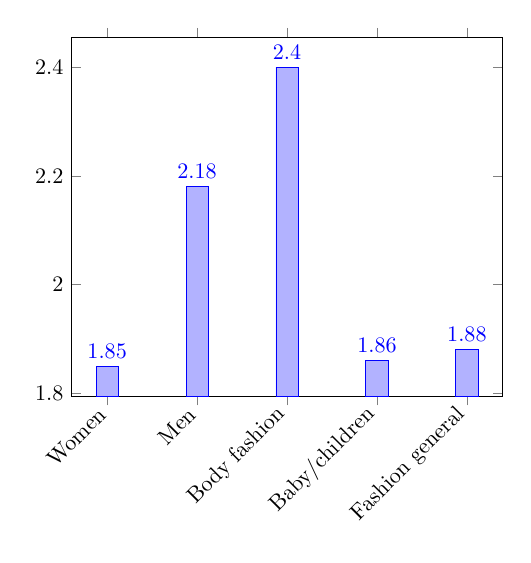
\begin{tikzpicture}[scale=0.8]
      \begin{axis}[
        ybar,
        symbolic x coords={Women, Men, Body fashion, Baby/children, Fashion general},
        x tick label style={rotate=45, anchor=east},
      ]
      \addplot +[nodes near coords] coordinates {
        (Women, 1.85)
        (Men, 2.18)
        (Body fashion, 2.40)
        (Baby/children, 1.86)
        (Fashion general, 1.88)
      };
      \end{axis}
    \end{tikzpicture}
    \caption{Conversion rate in various fashion segments}
\end{figure}

\marginpar{TODO: Conversion rate in SoBazaar?}
This figure is taken from~\cite{Jorij2012} and shows the conversion rate for
various segments in the fashion domain. The conversion rate is the portion of
users who visits a website, and reaches the target (makes a conversion) set
by the site. For most e-commerce application, SoBazaar included, a conversion
is counted when a purchase is made. The conversion rate $r$ can easily be
calulcated by $r = \frac{|Conversions|}{|Total visits|}$~\ref{nielsen2013}.
We can see that womens has the lowest conversion rate among the different
segments, indicating that there is a strong preference based shopping
tendency and that many users are \textit{browsing} and searching for the
right product. This hypthesis is strengthed by looking at the general
conversion rate in the e-commerce industry, which lies at 3\%. The potential
of a personalized recommender could in other words make browsing easier and
hence increase the conversion rate.

\begin{figure}[H]
  \begin{tabular}{cc}
    \resizebox{0.43\linewidth}{!}{
      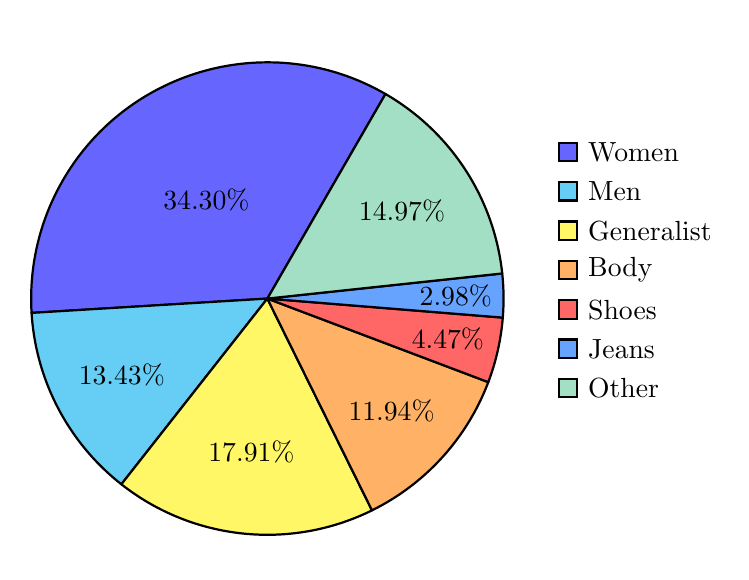
\begin{tikzpicture}
        \pie[text=legend, rotate=60]{
          34.30/Women,
          13.43/Men,
          17.91/Generalist,
          11.94/Body,
          4.47/Shoes,
          2.98/Jeans,
          14.97/Other
        }
      \end{tikzpicture}
    }
    \resizebox{0.49\linewidth}{!}{
      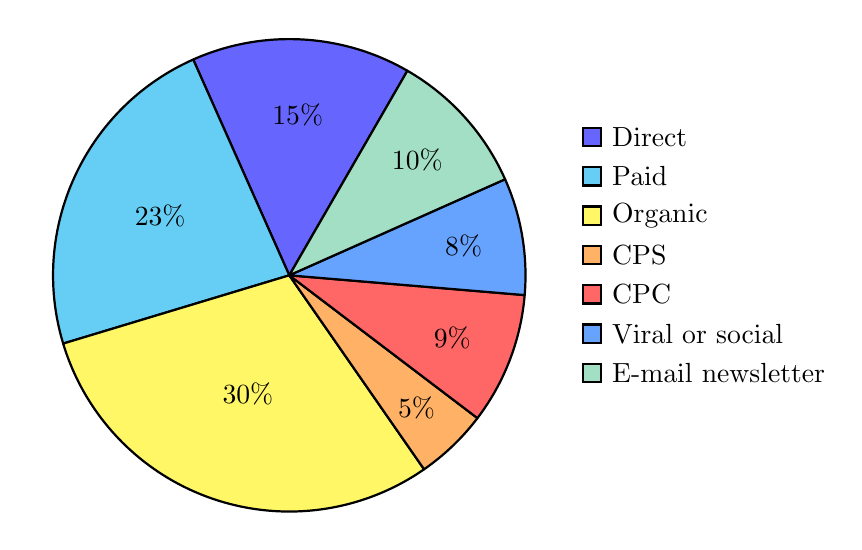
\begin{tikzpicture}
        \pie[text=legend, rotate=60]{
          15/Direct,
          23/Paid,
          30/Organic,
          5/CPS,
          9/CPC,
          8/Viral or social,
          10/E-mail newsletter
        }
      \end{tikzpicture}
    }
  \end{tabular}
  \caption{Distribution of target groups and traffic sources in the fashion
  domain}
\end{figure}

Both figures are taken from~\cite{Jorij2012}, basing its results from a study
with 70 participating fashion companies with the goal of doing a complete
benchmark of the industry. In the leftmost figure we see how the different
e-commerce fashion retailers focuses their products. We observe that a large
majority of e-commerce fashion companies are targeting women - as is
SoBazaar.  Underlining the comptetative market and the need to stand out to
the customer, by e.g. having personalized recommendations.

In the rightmost figure it is shown from where the customers originate in
online retails stores. The \textit{Paid} and \textit{Organic} are synonymous
with a user entering the site via. research or ads in the search engine, and
stands for 53\% of the traffic in e-commerce fashion - highlihting the
importance of a good reputation and digital profile. Direct traffic is as low
as 15\%, compared to the e-commerce industry in general where the same number
is 22.3\% \cite{Jorij2012}. This is explained by non-fashion products often
being offered in multiple stores and the users are thus browsing multiple
sites to find the best offer. Lastly we note that the viral/social segment is
rather small at 8\%, but compared to the e-commerce industry in general at
4\%. Hence we conclude that although a small of users interacts with fashion
companies by social media, it is a more important segment in this industry
compared to e-commerce in general.

\subsection{SoBazaar, the e-commerce application}
  As briefly mentioned in the introduction chapter~\ref{sec:motivation} SoBazaar is a fashion e-commerce application for web and hand held devices.
  The application is developed by Telenor and aggregates fashion products from various brands and stores, mainly fashion related.
  Users of the application can choose to log in with their social media account on Facebook~\footnote{Facebook is an online social media service with around 1.28 billion monthly active users~\cite{facebook}} to store and share their fashion findings in the application.
  This allows the user to have one entry point to get the latest updates on fashion, and see what the user's social network is up in regards to fashion.
  When the user finds an item especially interesting and is interested in purchasing the item, the user is redirected to the store from which the product originated.

  The fact that SoBazaar utilizes Facebook and a large set of fashion stores lets the users of the application gather at one place to find users with similar taste in fashion.
  As seen from~\ref{subsec:theory} one important aspect in fashion is the feeling of belonging, which is made easy through the utilization of Facebook.

\subsection{Competitors to SoBazaar}
  \label{subsec:competitors}

	\marginpar{TODO: Extend with Asos}
	\marginpar{TODO: Extend with Kwoller}
	\marginpar{TODO: Extend with Mallzee}
	\marginpar{TODO: Mention that many new apps have popped up recently, attempting to do the same as SoBazaar}

    As seen from~\ref{subsubs:fashionInEcom} SoBazaar is not the only e-commerce application for fashion, and has therefore some competitors.
    SoBazaar is built up of a collection of e-commerce store front applications and social interactions, but SoBazaar is not the first of its kind.
    There is a set of other similar applications providing the user with similar possibilities as SoBazaar.
    This section will be used to explore some of these systems, and look into their strengths and weaknesses regarding item recommendation for the user.

\subsubsection{Myntra} % (fold)
\label{par:myntra}
    "Myntra.com is a one stop shop for all your fashion and lifestyle needs" - about Myntra~\cite{myntra}.

    Myntra is one of India's largest e-commerce stores for fashion and aims to  provide a hassle free shopping experience for the user.
    They aim to bring the newest and most in-season fashion products available to the user trough the web store front.
    The brand base of Myntra consists of 500 leading brands from both inside and outside India.

    The web page uses a set of recommendation approaches to inform the user of what they might like, and to increase the user's awareness of different kinds of items. Such as, similar item and most popular.

    \begin{figure}[H]
        \centering
        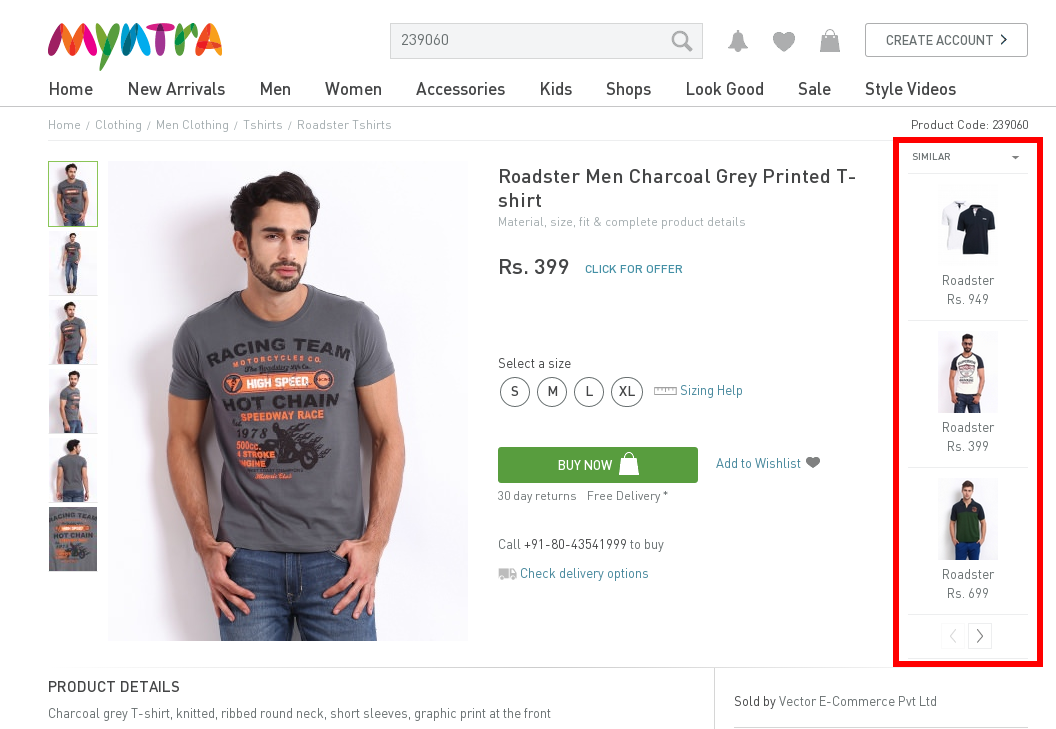
\includegraphics[width=5in]{image/myntiaSimilarExample.png}
        \caption[Example of Myntra's "similar item" approach]{In this figure we can see in red how Myntra is suggesting items which are similar to the item the user is currently looking at}
        \label{figure:myntiaSimilarEx}
    \end{figure}

    \begin{table}[H]
        \centering
        \begin{tabularx}{\linewidth}{>{\parskip1ex}X@{\kern4\tabcolsep}>{\parskip1ex}X}
            \toprule
            \hfil\bfseries Strengths
            &
            \hfil\bfseries Weaknesses
            \\\cmidrule(r{3\tabcolsep}){1-1}\cmidrule(l{-\tabcolsep}){2-2}
            %Strengths
	        Suggest similar items connected to the currently viewed \par
            Popular list for the different brands and stores \par
            Ability to add item to a "want list"\par
            &
            %Weaknesses
            No personalized recommendations \par
            \\\bottomrule
        \end{tabularx}
        \caption[Recommendation related strengths and weaknesses of Myntra~\cite{myntra}]{This table is the list of the recommendation related strengths and weaknesses of the e-commerce fashion web site Myntra~\cite{myntra}}
        \label{table:ecommerceMyntra}
    \end{table}
% paragraph myntra (end)

\subsubsection{Lyst} % (fold)
\label{par:lyst}
    "Lyst.com is a fashion shopping site that gives you your own shopping experience, so you can discover more of the fashion you love" - About Lyst~\cite{lyst}.

    Lyst offers items from thousands of the leading brands and stores of the world.

    The site allows the user to follow different stores or brands to receive the latest items they have to offer.
    The user is given a personalized "stylefeed", which displays items from the different brands or stores the user is following.
    It is also possible for the user to add items to the their profile.

    On first login the user is presented with a set of brands and store the user can like or dislike, to get the "stylefeed" started.
    On access of an item, the user is presented with related items, and the ability to add the item to a collection.
    When the user wants to buy an item, the site will redirect the user to the store selling the item.

    \begin{table}[H]
    	\centering
        \begin{tabularx}{\linewidth}{>{\parskip1ex}X@{\kern4\tabcolsep}>{\parskip1ex}X}
        \toprule
        	\hfil\bfseries Strengths
            &
            \hfil\bfseries Weaknesses
            \\\cmidrule(r{3\tabcolsep}){1-1}\cmidrule(l{-\tabcolsep}){2-2}
                    Can follow brands and stores \par
                    Connected with facebook \par
                    Ability to add item to a "want list" \par
                    "Stylfeed" based the user's follow list \par
                    Show related items \par
                    &
                    Limited personalized recommendations \par
                    \\\bottomrule
                \end{tabularx}
        \caption[Recommendation related strengths and weaknesses of Lyst~\cite{lyst}]{This table is the list of the recommendation related strengths and weaknesses of e-commerce fashion web site Lyst~\cite{lyst}}
        \label{table:ecommenreceLyst}
    \end{table}
% paragraph lyst (end)

\subsubsection{Farfetch} % (fold)
\label{par:farfetch}
    "farfetch.com forms the hub of a global fashion community that unites independent boutiques around the world with fashion lovers" - About Farfetch~\cite{Farfetch}

    Farfetch is a collection of over 1000 boutiques from all over the world gathered on one web page.
    The user can shop directly on the page, and get the item delivered to the doorstep with only one checkout process.

    When browsing an item the user is presented with a set of recommendations related to the current item, and previous browsing history.
    The item can be added to a "want list" or to the shopping chart.
    \begin{figure}[H]
        \centering
        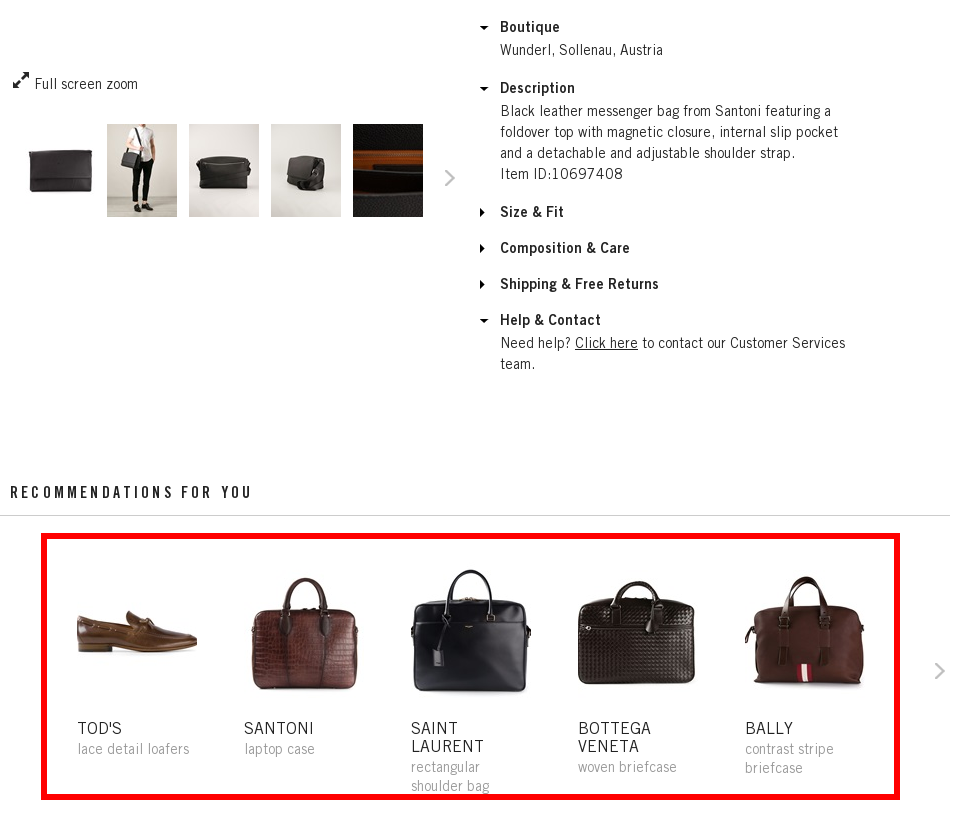
\includegraphics[width=5in]{image/farfetchedRecommendationExample.png}
        \caption[Example of Farfetch's recommendations]{In this figure we can see in red how Farfetch is recommending items which might be of interest to the user. As we can see the first item is a shoe, which was the last item accessed by the user, the next four items are related to the currently viewed item}
        \label{figure:farfetchedRecommendationExample}
    \end{figure}
    \begin{table}[H]
        \centering
        \begin{tabularx}{\linewidth}{>{\parskip1ex}X@{\kern4\tabcolsep}>{\parskip1ex}X}
        	\toprule
        	\hfil\bfseries Strengths
        	&
        	\hfil\bfseries Weaknesses
        		\\\cmidrule(r{3\tabcolsep}){1-1}\cmidrule(l{-\tabcolsep}){2-2}
        		%Strengths
                Ability to add item to a "want list" \par
                A feed with the most popular items \par
                A feed with new items \par
                A list of recommendations for the user \par
            	&
            	%Weaknesses
                No option to follow other users \par
             \\\bottomrule
        \end{tabularx}
        \caption[Recommendation related strengths and weaknesses of Farfetch~\cite{Farfetch}]{This table is the list of the recommendation related strengths and weaknesses of e-commerce fashion web site Farfetch~\cite{Farfetch}}
        \label{table:ecommenreceFarfetch}
    \end{table}
% paragraph farfetch (end)

\subsubsection{MyHabit} % (fold)
\label{par:myhabit}
    "MyHabit is a private fashion sale site offering up to 60% off hand-picked selections from designer and boutique brands." - About MyHabit~\cite{MyHabit}

    MyHabit was founded by Amazon in response to the desire from the users of Amazon to shop fashion in an easy manner.

    The site displays a feed.
    This feed is fed by a team from MyHabit, and is constantly updating with new sales and new products.
    The items put into the feed are handpicked.

    When browsing items on MyHabit, other similar items are suggested to the user.
    \begin{table}[H]
                    \centering
                    \begin{tabularx}{\linewidth}{>{\parskip1ex}X@{\kern4\tabcolsep}>{\parskip1ex}X}
                    \toprule
                    \hfil\bfseries Strengths
                    &
                    \hfil\bfseries Weaknesses
                    \\\cmidrule(r{3\tabcolsep}){1-1}\cmidrule(l{-\tabcolsep}){2-2}
                Shop on site \par
                Similar items \par
             &
                No personalized recommendations \par
            \\ \bottomrule
        \end{tabularx}
        \caption[Recommendation related strengths and weaknesses of MyHabit~\cite{MyHabit}]{This table is the list of the recommendation related strengths and weaknesses of e-commerce fashion web site MyHabit~\cite{MyHabit}}
        \label{table:ecommenreceMyHabit}
    \end{table}
% paragraph myhabit (end)

\subsubsection{Competitors Recommendation Overview} % (fold)
\label{par:competitors_recommendation_overview}
    In table~\ref{table:ecommerceCommpetiros} we see that there is a very low count of fashion related e-commerce applications, which actually produces personalized recommendations for their users.

    Most of applications are taking a simpler approach when making recommendations for the user, like most popular or similar items.
    There is no obvious relation between recommendations and that the site has a form of "want list", but the system which allows the users to follow each other are usually not in-application-purchase-applications.

    There where no indications of the "want list" being used directly to some personalized recommendations and neither was it any indication that the "follow list" of other users helped produce any personalized recommendations, other than recommending items from the followed user's feed.
    The "follow list" was also in some cases used to suggest other users to follow.
    The "want list" was primarily there so that the user could go back to a liked item, and maybe interact with it later.
    \begin{table}[H]
        \centering
        \begin{tabular}{l l l l l l l}
            \toprule
            Competitor &
            \multicolumn{1}{l}{\parbox{1.3cm}{ In App \\ Purchase}} &
            \multicolumn{1}{l}{\parbox{1.0cm}{ Most \\ Popular}} &
            \multicolumn{1}{l}{\parbox{1.0cm}{ Similar \\ Items}} &
            \multicolumn{1}{l}{\parbox{1.0cm}{ Want \\ List}} &
            \multicolumn{1}{l}{\parbox{1.9cm}{ Follow \\ Other Users}} &
            \multicolumn{1}{l}{\parbox{2.6cm}{ Personalized \\ Recommendations}} \\ \midrule

            Myntra  & \cmark & \cmark & \cmark & \cmark & \xmark & \xmark \\
            Flink   & \xmark & \cmark & ?? & \cmark & \cmark & \xmark \\
            Lyst    & \xmark & \cmark & \cmark & \cmark & \cmark & \xmark \\
            Motilo  & \xmark & \cmark & \xmark & \cmark & \cmark & \xmark \\
            Farfetch & \cmark & \cmark & \cmark & \cmark & \xmark & \xmark/\cmark~\tablefootnote{How the recommendations are produced is not mentioned} \\
            ModCloth  & \cmark & \cmark & \cmark & \cmark & \xmark & \xmark \\
            UsTrendy  & \cmark & \cmark & \cmark & \cmark & \xmark & \xmark \\
            Polyvore  & \xmark & \cmark & \cmark & \cmark & \cmark & \xmark \\
            Clothia  & \xmark & \cmark & \cmark & \cmark & \cmark & \xmark \\
            Trendabl  & \cmark & \cmark & \cmark & \cmark & \cmark & \xmark \\
            Zalando  & \cmark & \cmark & \cmark & \cmark & \xmark & \xmark \\
            Ellos  & \cmark & \cmark & \cmark & \cmark & \xmark & \xmark \\
            LookBook  & \xmark & \cmark & \cmark & \cmark & \cmark & \xmark \\
            Fahsiolista  & \xmark & \cmark & \xmark & \cmark & \cmark & \xmark \\
            ShopStyle  & \xmark & \xmark & \cmark & \cmark & \xmark & \xmark \\
            MyHabit  & \cmark & \xmark & \cmark & \xmark & \xmark & \xmark \\
            \bottomrule
        \end{tabular}
        \caption{Properties of different e-commerce application}
        \label{table:ecommerceCommpetiros}
    \end{table}
    Show in the table~\ref{table:ecommerceCommpetiros} above is the list of the different properties of some of the different competitors to SoBazaar. The properties are in regards of their recommendation ability, and how they let their user expand their item set
    A more complete list can be found in the appendix~\ref{app:sec:soCompetitors}.

% paragraph competitors_recommendation_overview (end)

% mtodo
% Diskusjon
%   behold 3 resten til appendix
      % utdyp om SoBazaar, hvordan passer de inn
      % Bruk data til å beskrive at det vi driver med er viktig.
%   Hvborfor har vi dette?
%   Dert er få anbefalinger
%   Dollars er et lukurativt market

  % Heri satte utropstegn ved:
  %   Flink
  %   Lyst og
  %   Motilo

\subsection{Fashion Recommender Systems}
    This subsection will look at different methods other fashion related systems have used to recommend fashion related products to the user.

\subsubsection{Photograph based approach}
    Fashion and the products it regards are highly dependent on visuals.  A fashion
    product would not be very interesting if no one saw it.  An approach to use the
    importance of how the product looks regarding recommending is to utilize images
    of the product.  Fashion Coordinates Recommender System Using Photographs from
    Fashion Magazines~\cite{Iwata:2011} is a system doing this.  They teach their
    system by using fashion magazines with full body images.  They segment the
    image into two parts, top and bottom.  From this the system learns which top
    matches to which bottom and collects visual features of the products.  From
    this the system can recommend other tops to go with a selected bottom, or other
    way around.  The proposed system scored better\footnote{Accuracy of 50\% on the
    top 5 suggested items, whereas naive and random managed 18\% and under 5\%
    respectively} than both a more naive approach and a random selection.  Runtime
    was at 0.04 seconds per recommendation.

\subsubsection{Hot-or-not}
    A recommender system called SuitUp~\cite{SuitUp} did a survey on some of their potential users.
    One interesting finding was that many of the users enjoyed the Hot-or-Not feature of the system.
    This feature gives the user a set of items and the option to either like or dislike.
    This did not only make the participants in the survey more engaged in the system, but also produced ratings, both negative and positive, for the system.
    For cold-start users and in a cold-start system this extra information and ratings make it much easier to make recommendations for the users.

\subsubsection{Scenario-Oriented Recommendation}
    Shen et al.~\cite{Shen:2007:AIG:1216295.1216368} proposed a recommender system which produce recommendations not only based on the metadata of the products, but also on user written input.
    Knowledge used to handle the user input, is derived from Open Mind Common Sense~\cite{Singh02openmind}.

    The user uploads his or her clothes and adds brand (e.g.Nike), type (e.g.jeans), material and a description about the item (e.g."I put these on when I get home").
    The systems makes recommendations based on the scenario the user is needing help to find suiting clothes to wear.
    The typical use case of the system is when a user is unsure about what to wear under different circumstances, but knows something about the scenario or occasion the clothes will be worn in.
    For instance: "I am going to the beach".
    It is also possible to interact with other users and the system relates similar users.

    The different describing fields about the items are given a six-tuple style value.
    The six tuples are: luxurious, formal, funky, elegant, trendy and sporty, where each is given a value from 0 to 10 based on how much the describing field of the items is the current tuple.
    The different describing fields are given a default value, which can be changed by the user if that this necessary. But it seems like this has to be done for all brands, material and type manually to initialize the system.

    This is an interesting approach to fashion and clothes recommendations but the need for user scenario input and a six-tuple description of the different describing fields, might not be desirable for the user or the system administrator in the long run.

    Yu-Chu et al.~\cite{Yu-Chu:2012:PCS:2376365.2376961} and Ying et al.~\cite{Ying2011} are other similar systems. Ying et al.~\cite{Ying2011} made a recommender based on the a similar concept, namely, what to wear in different situations.
    The system recommends two sets of top-to-toe clothing based on the current season, the occasion and the items the user has uploaded.
    The uploaded items must be given a set of descriptions, including the occasion to use the item.

    To recommend, the system uses the user profile of the user, which describes the interests of the user and the information given by the user about the different items in his or hers wardrobe.

\subsubsection{Photograph Recommendation Integrated with Occasion} % (fold)
\label{par:photograph_recommendation_integrated_with_occasion}
    Liu et al.~\cite{Liu:2012:HMC:2393347.2393433} combined the two approaches from Iwata et al.~\cite{Iwata:2011} and Ying et al.~\cite{Ying2011} and Shen et al.~\cite{Shen:2007:AIG:1216295.1216368} and suggested a system which recommend clothes both based on the photographies and the occasion the clothes are to be worn.

    They do this by incorporating fashion rules like, what can you wear to which occasion, and what can you wear as a complete set to different occasions.
    The recommender learn the clothing recommendations through a latent support vector machine framework.
    They use this framework to match four potential functions: visual features vs. attribute, visual features vs. occasion, attributes vs. occasion and attribute vs. attribute.
    These are used together in a scoring function for clothing recommendation.

    Their system preformed better than the baselines, but was highly dependent on the human detection accuracy, since the learner was learning from fashion photographs.
% paragraph photograph_recommendation_integrated_with_occasion (end)

% !TEX root = ../../report.tex

\section{Session Based Approach}
    Different ways of personalizing recommendations have been explored earlier in this chapter, such as: collaborative filtering and content based filtering.
    A common issue with these types recommendations is sparsity in the data, which can lead to poor recommendations.
    Through utilizing usage pattern of the user and producing sessions, some of the sparsity gaps can be filled.
    The patterns can help to understand the pre-purchase patterns, products they see and what they buy.
    This information can also produce interesting relationships between products.
    With this the user preferences can be gathered and be used to reduce the search space when recommending product for the user.

% \subsection{E-commerce}
%     About sessions

\subsection{Mining}
    How to gather information on the user.
    The data mining can be split into two main steps~\cite{Cho2002329}:
    \begin{itemize}
        \item \emph{Data Preparation} - In the data preparation step the sessions are built. They are built based on the usage during a single visit to the application, web page or system the user is accessing. It is the sequence of events produced by the user actions during the visit.
        \item \emph{Pattern Discovery} - In the pattern discovery step the system must use the sessions gathered in the previous step to discover association rules, sequential patterns, usage clusters, page clusters, user classification or any other pattern discovery method.
    \end{itemize}

    \subsubsection{Data Preparation} % (fold)
        \label{par:Data_Preparation}
        When a user accesses an application or web page, the system can store the footprints of the user.
        Within these footprints the system can embed information as browser used by user, location of the user, event triggered by user and time stamp.
        This bundle of information is called an event, a the set of event produced by the user during on application or web page visit, is called a session.

    \subsubsection{Pattern Discovery} % (fold)
        \label{par:pattern_discovery}
        \paragraph{Association Rules} % (fold)
            \label{subp:association_rules}
            The association rule describes how item X and Y are coupled, this coupling is the percentage of transactions that contain both item X and item Y.

            One simple way of discovering this association is through the aprior algorithm~\cite{Agrawal:1994:FAM:645920.672836}.

            With this set of rules for the items, item taxonomies can be used to infer knowledge regarding the items.
            For instance; sessions when buying blue skirts often include buying of red shoes.
        % easy example: http://nikhilvithlani.blogspot.no/2012/03/apriori-algorithm-for-data-mining-made.html
        \paragraph{Sequential Patterns} % (fold)
        \label{subp:sequential_patterns}
            The sequential patterns can be used to build Markov models to predict the next step the user will take based on the sequential pattern of the events from the sessions~\cite{Deshpande:2004:SMM:990301.990304}.

            An issue with using the Markov model is that if first-order is being used, the accuracy can be faulty, since the model will not be looking far enough behind.
            Handling this with an higher-order model might solve the inaccuracy due to too low order, but might cause an issue with high state space complexity, and might also reduce coverage.
            Which can be handled through training a set of K different Markov models, with K different orders, All-$K^{th}$-Order Markov model, but the space complexity issue will still be present.

            The Markov model predicts future actions through looking at past actions.
            So for first-order, the model looks at the last event performed to predict the next event of the user.
            The higher the order, the further back the model is looking in the event set and will produce a more complicated model, the higher the order.
            This can be handled through the usage of a selective Markov model~\cite{Deshpande:2004:SMM:990301.990304}

            One issue with the Markov model is that a user will not get predicted new items if the sessions used to predict future actions are only based on the own users sessions.
            One way of making use of the patterns and producing new recommendations is trough matching sequential patterns from users with one-another. \marginpar{something not right}


        \paragraph{Usage Clusters} % (fold)
        \label{subp:usage_clusters}
            The usage clusters are usually built up from the different features of the events in the session.
            Where the features are collected an used to model the user.

            \begin{table}[H]
                \centering
                \begin{tabular}{l|l}
                    \emph{Event features} & \emph{Description} \\ \hline
                    Amount of purchases & - \\ \hline
                    Amount of viewsts & - \\ \hline
                    Amount of wants & - \\ \hline
                    Time on items under the different conditions mentioned above & -\\ \hline
                    Overall average time on items & - \\ \hline
                    Click to buy rate & - \\ \hline
                    Search query~\cite{Zhang:2006:MSE:1135777.1136004} & - \\ \hline
                    What was done before a specific action & - \\ \hline
                    What was done before a specific action & - \\
                \end{tabular}
                \caption[Event Features]{Set of event features used for finding usage clusters and model the users behavior}
                \label{table:uasageCluster}
            \end{table}

        \paragraph{Page Clusters} % (fold)
        \label{subp:page_clusters}
            Page clustering will help the system to understand which pages belong together.
            For instance when searching for Harry Potter, the user might have interest in knowing more about the author J.K. Rowling, and the system might benefit from clustering queries of here with Harry Potter~\cite{Zhang:2006:MSE:1135777.1136004}.

        % \paragraph{User Classification} % (fold)
        % \label{subp:user_classification}

\subsubsection{Session Examples} % (fold)
    \label{par:session_examples}
    \marginpar{Show three common user session patterns (average purchase time, want time and view time)}
    A user session of a user randomly chosen user.
    \begin{lstlisting}
        { "event_id" : "app_started", "product_id" : "NULL", "ts" : NumberLong("1382689141084") }
        { "event_id" : "storefront_clicked", "product_id" : "NULL", "ts" : NumberLong("1382689144152") }
        { "event_id" : "storefront_clicked", "product_id" : "NULL", "ts" : NumberLong("1382689172026") }
        { "event_id" : "storefront_clicked", "product_id" : "NULL", "ts" : NumberLong("1382689179152") }
        { "event_id" : "product_detail_clicked", "product_id" : 2028030, "ts" : NumberLong("1382689192035") }
        { "event_id" : "product_purchase_intended", "product_id" : 2028030, "ts" : NumberLong("1382689197749") }
        { "event_id" : "product_detail_clicked", "product_id" : 2038024, "ts" : NumberLong("1382689263384") }
        { "event_id" : "storefront_clicked", "product_id" : "NULL", "ts" : NumberLong("1382689284693") }
        { "event_id" : "storefront_clicked", "product_id" : "NULL", "ts" : NumberLong("1382689297864") }
        { "event_id" : "storefront_clicked", "product_id" : "NULL", "ts" : NumberLong("1382689322201") }
        { "event_id" : "storefront_clicked", "product_id" : "NULL", "ts" : NumberLong("1382689326804") }
        { "event_id" : "storefront_clicked", "product_id" : "NULL", "ts" : NumberLong("1382689352841") }
        { "event_id" : "product_detail_clicked", "product_id" : 2028032, "ts" : NumberLong("1382689357563") }
        { "event_id" : "product_detail_clicked", "product_id" : 2038025, "ts" : NumberLong("1382689363957") }
    \end{lstlisting}

    purchase time: 14068.69687
    want time: 17859.1539

% ~\cite{Kelly:2003:IFI:959258.959260}


\subsubsection{Multi-Armed Bandit} % (fold)
    \label{par:multi_armed_bandit}
    \marginpar{might be interesting as an most popular approach, suggest the most popular at any one time, belongs with most popular approach}

\subsubsection{Analyzing}
    Analyzing the model of the user

\subsection{Recommending}
    Using the model to help personalizing the recommendation for the user

\subsection{Limitations}
    What are the limitations of a session based approach to recommendations.


% % !TEX root = ../../report.tex
\section{One-Class Collaborative Filtering}

% todo - hva vil vi med denne sekjsonen?

\subsection{About}
    There are many applications where the feedback from a user is in binary form.
    Take for instance a item purchase page without explicit feedback.  The only
    feedback from a user might only be if an item has been purchased or not, the
    data consists only of binary data.  Other cases can include page visitation or
    webpage bookmarking.  The fallout of this is that the data collected from the
    user is usually really sparse.  And one issue which arises from the binary
    feedback is the lack of known negative feedback.  Does the fact that a user
    visited a web page, but not another indicate that the user dislikes the
    unvisited page, or simply that the user oversaw it?  The negative feedback and
    the missing feedback are mixed together in the bigger part of the dataset.
    Which makes it difficult to identify what is what.  Recommendations, through
    finding the missing positives, done on these types of data is usually thought
    of as one-class collaborative filtering (OCCF).  OCCF can be viewed as an
    extreme case of class imbalance, in which the balance is only distributed over
    one class. \marginpar{checkout Extreme re-balancing for svms: a case study
    maybe}

\subsubsection{Common OCCF Scenarios}
    Some of the most common scenarios where the OCCF problems occurs are:
    Bookmarking, click history, product purchase, "like" and news reader.  The data
    produced from user feedback from all these scenarios can be on the binary form.

\subsection{Different approaches}
    To handle the problem with the sparse data mixed with the ambiguous missing
    data, several strategies has been proposed.

\subsubsection{Negative ratings}
    Since one of the main issues are with the missing data, a natural approach
    would be to gather more.  One way of doing so is by asking the user to rate
    more items.  This can be done through forcing the user to rate a set of
    predetermined items and/or produce negative ratings to uninteresting items.
    The issue with this approach is that putting the rating burden onto the user
    has shown to produce negative user
    experience~\cite{Kelly:2003:IFI:959258.959260}

\subsubsection{All missing as negative (AMAN)}
    One naive approach is to view all the missing values as negative values.
    Thereby saying all web pages ignored by the user are unwanted pages.  One issue
    with this approach is that it will render examples which are positive, but
    unknown, as false negatives.

\subsubsection{All missing as unknown (AMAU)}
    Another naive approach is to go in the opposite direction.  Viewing all missing
    values as unknown, thereby only utilizing the known values when recommending,
    the predictions on the unknown values will only be positive.  The data in an
    OCCF problem is also usually very sparse, therefore using only the positive
    examples will in many cases lead to an incomplete view of the data, and quality
    reduced recommendations.

\subsubsection{Weighted low-rank approximation}
    \cite{pan2008} \cite{Nati03weightedlow-rank}
    The idea behind this approach is to distribute different weights to the unknown
    values.

    More specifically, given two matrices, one rating matrix $R = SxC$, where $S$
    is a list of $m$ items, $S = {s_{1},...s_{m}}$ and $C$ is a list of $n$ users,
    $C = {c_{1}, ... c_{n}}$.
    $R$ has a corresponding weight matrix $W$, where $S$ is a list of $m$ items, $S
    = {s_{1},...s_{m}}$ and $CWz$ is a list of $n$ users, $C = {c_{1}, ... c_{n}}$.
    The values in $R$ are either 0 or 1, and the values in $W$ are between 0 and 1.
    With these two matrices, weighted low-rank approximation is meant to find a low
    rank matrix $X$.  Done through the Frobenius norm, which is minimizing the sum
    squared differences to the target matrix~\cite{frobeniusNorm}.  Other
    approaches to the weighting issue has been taken, such as low-density
    non-negative matrix factorization~\cite{Sindhwani:2010:OMC:1933307.1934641}.

    \begin{equation}
        J(X) = \sum_{mn} W_{mn}(R_{mn} - X_{mn})^2
        \label{equation:frobenius}
    \end{equation}

    Equation~\ref{equation:frobenius} can be optimized and solved efficiently
    though the use of wighted ALS~\citep{Koren2009}.  The positive values are set
    to 1 in the $R$ matrix, and the negative set to 0.
    Since the positive values have a high certainty of being correct, the
    corresponding wight from the matrix $W$ is set to 1.  For the unknown values
    the corresponding weight is set after a weighting schema.  Where the weight is
    lowered for more certain negatives.  This weight is between 0 and 1.  Another
    approach to handling the

    \begin{table}[H]
        \centering
        \begin{tabular}{l|l|l}
          \emph{Schemes}      & \emph{Pos Examples} & \emph{Neg Examples} \\ \hline
          Uniform               & $W_{mn} = 1$ & $W_{mn} = [0,1]$ \\ \hline
          User-Oriented         & $W_{mn} = 1$ & $W_{mn} = UO(\sum_{n} R_{mn})$ \\ \hline
          Item-Oriented         & $W_{mn} = 1$ & $W_{mn} = IO(m - \sum_{n} R_{mn})$ \\ \hline
          User-Item interaction & $W_{mn} = 1$ & $W_{mn} = E(I)$  \\ \hline
          User-Item similarity & $W_{mn} = 1$ & $W_{mn} = S(I,U)$  \\
        \end{tabular}
        \caption[Weighting Schemes]{Different ways of weighting ratings suggested by \cite{pan2008}}
        \label{table:WeightingSchemes}
    \end{table}

    Different weighting schemes are show in~\ref{table:WeightingSchemes}.

    The uniform approach considers all negative examples in the same way, and
    thereby assigns the same weight to all the negative examples.  The
    user-oriented scheme assumes that if a user has more ratings, the negative
    examples can be weighted to be more negative.  The item-oriented assumes that
    if there are more positive example for an item, the missing data is negative
    with a lower probability.  The last scheme, the user-item interaction
    approach, takes into consideration the events on the item to be considered.
    For instance clicks and views.

    \paragraph{User-Item similarity} % (fold)
        \label{subp:user_item_similarity}
        In the user-item similarity approach, the items content of the items and from the users are extracted based on the examples in the data where the positive examples are set to 1.
        From this there is built models for the users and the item.
        The similarity between the user and the item is then used to give the negative examples a weight~\cite{yuan2013}.

\subsubsection{Negative example sampling~\cite{pan2008}}
    In many cases the missing values are in fact negative values.  This approach
    will i most cases lead to a large rating matrix, and therefore high
    computational costs.  Therefore, instead of using all the ratings in the
    ratings matrix $R$, only all the actual positive values are selected.  This is
    combined with a subset of the presumed negative values.  This subset is based
    on a sampling probability matrix $P$.

    There are different sampling schemes.
    Using the same schemes as from weighted low rank approximation.

\subsubsection{Group Bayesian personalized ranking (GBPR)~\cite{Pan:2013:GGP:2540128.2540516}}
    Utilizing rich user interaction.  Group preference is the preference score of a
    group of user on an item.  GBPR assumes that the group preference is stronger
    than the observed user preference.

\subsubsection{Incorporating Rich User Information~\cite{deLace2010,Li2013}}
    When dealing with implicit feedback extra information is usually available
    regarding the user and item.  For instance search query, click history, view
    time and purchase history.  Two ways of incorporating this information has been
    proposed in~\cite{deLace2010}.  One is through linearly combining cores from
    the different sources, and the other is through embedding user information into
    collaborative filtering.

% \subsubsection{Em algorithms to predict negative examples}
    % \cite{Nati03weightedlow-rank}
    % % \todo{check out the approaches}
    % PEBL: positive example based learning for web page classification using SVM
    % Building text classifiers using positive and unlabeled examples
    % Presence-only data and the EM algorithm

    % \subsubsection{Low-density non-negative matrix factorization (ldNMF)}
    % \cite{Sindhwani:2010:OMC:1933307.1934641}
    % arg min
    % J W, H, {y ij } (i,j)∈U =
    % W ≥0,H≥0
    % y ij ∈{0,1},(i,j)∈U
    % λ W
    % 2
    % F
    % + γ H
    % 2
    % F
    % C ij V (X ij , w i T h j )
    % +
    % (i,j)∈L
    % C ij V (y ij , w i T h j )
    % +
    % (i,j)∈U
    % % \todo{make equation}
    % Equation.
    % $R = SxC$ % \todo{0 or 1} is the rating matrix, where $S$ is a list of $m$ items, $S = {s_{1},...s_{m}}$ and $C$ is a list of $n$ users, $C = {c_{1}, ... c_{n}}$.
    % $L$ is the set of positive ratings, while $U$ is the set of unlabeled rating.
    % $W$ and $H$ are the latent factors.
    % $V$ is a loss function (squared loss or generalized KL-divergence).
    % $C$ is the entry specific costs.
    % γ ≥ 0 and $λ$ tradeoff the regularizers againts the fata-fit terms.

\subsection{Discussion}
% todo discuss

% !TEX root = ../../report.tex
\section{Evaluation}
\label{evaluation}

	% What evaluation methodologies exist?
		% Offline Evaluation
		% 	Recommender System Datasets
		%		Explicit vs. Implicit
		% 	Offline Evaluation Measures
		%		Traditional evaluation measures
		%		Cold-start system evaluation
		%		Implicit feedback evaluation measures
		% Online Evaluation


%Some key questions in evaluating recommender systems on testbed data are: what
%to predict, how to grade performance and what baseline to compare with.

In most cases a system designer that wish to employ a recommender system must
choose between a set of candidate approaches. A first step towards selecting an
appropriate algorithm is to decide which properties are the most important for
the application. Recommender systems have a variety of properties such as
accuracy, robustness, scalability, etc. The following section will discuss how
to compare recommender systems based on the set of properties  relevant for the
application and how to evaluate the performance of the system. We have several
different experimental settings which can be used to evaluate recommender systems.
We will focus on two types of experiments:
Offline experiments where the system is evaluated without user interactions and
Online experiments where real users interact with the system. This section will
also cover some of the most frequently used evaluation metrics, a discussion on
the suitedness of different evaluation measures for implicit feedback, and
summary of the methodologies and evaluation measures used to evaluate the
cold-start performance of recommender systems.

Shani et al.\ \cite{Shani2011} lists the following guidelines for general
experimental studies:

\begin{itemize}
	\item Hypothesis: before running an experiment one must form an hypothesis. For
		example, an hypothesis can be that algorithm $A$ better predicts user ratings
		than algorithm $B$. In that case the experiment should test the prediction
		accuracy, and not look at other factors.

	\item Controlling variables: when comparing a few candidate algorithms on a
		certain hypothesis, it is important that all variables that are not tested
		are fixed.

	\item Generalization power: when drawing conclusions from experiments, we may
		wish that our conclusions generalize beyond the immediate context of the
		experiments. When choosing an algorithm for a real application, we may want
		our conclusion to hold on the deployed system, and generalize beyond the
		experimental data set. To increase the probability of generalization of the
		recommender results one must typically experiment with several data sets or
		applications.
\end{itemize}

\subsection{Offline Evaluation}
Offline experiments are performed using pre-collected dataset\(s\) and a protocol
that models the user behavior to estimate recommender performance through
different evaluation measures. Offline experiments are attractive because they
require no interactions with real users, and thus allows multiple  researchers to compare
a wide range of algorithms, using the same data, at a low cost. The downside of offline experiments
is that they can answer a very narrow set of questions, typically questions
about the predictive power of the algorithm, and does not measure other user
factors.

\subsubsection{Datasets for Offline Evaluation}

The main aim of a recommender system is to identify the set of items in a
dataset that might be interesting to a user based on their expressed
preferences. For a fashion recommender this would mean estimating how much a
user might like an item, by e.g.\\ predicting what rating a user might give an
item. In recent years, various test collections for different domains such as
books, music, movies have been made available to the public. These datasets
usually consist of user ratings in the form of $(UserID, ItemID, Rating)$,
but may also include a timestamp.

In recent years more or more datasets have been made available which contains
additional information such as demographic information about the users,
trust-networks, user-assigned tags and etc. Under we have listed a few selected
popular datasets containing additional information:

%TODO - Find more cool dataset

\begin{itemize}

\item MovieLens 100k dataset~\cite{Movielens}: The movielens dataset
	incorporates demographic information about the user in addition the
	traditional rating matrix

\item Epinions dataset~\cite{Epinions}: The Epinions dataset includes a
	trust-network, which specifices who-trust-whom in a social network based on
	customer reviews for the website Epinions.com

\item The Million Song Dataset~\cite{Bertin-Mahieux2011}: The million song
	dataset is a implicit feedback dataset. This data also includes information on the users,
	and audio features and song meta-data.

\item The Book-Crossing Dataset: The bookcrossing dataset consists of both implicit and explicit feedback,
	demographic information about users and some content based information about the books.
\end{itemize}

\paragraph{Explicit-feedback}
The definition of explicit is defined as `stated clearly and in detail, leaving
no room for confusion or doubt'. Explicit feedback are more precise than
implicit feedback, but more difficult to collect since it requires active user
involvement. One serious implication of this is that the amount of feedback
often is scarce since many users opt not to provide any feedback. Explicit
feedback mechanisms allow the users to unequivocally express their ratings on a
scale (usually in the form of a Likert scale (strongly disagree – strongly
agree). Thus explicit feedback is able to capture both negative and positive
feedback, while implicit feedback \emph{only} can be positive. It is worth
noting that explicit feedback tend to concentrate on either side of the rating
scale, as users are more likely to express their preference if they feel
strongly for or against an item~\cite{Jawaheer2010}.

\paragraph{Implicit-feedback}
Unlike explicit feedback, we do not have any direct input from the user
regarding their personal preferences. In particular we do not have any
substantial evidence of which items the user dislikes, such as low ratings.
What we do have is indications of whether a user likes an item trough clicks, wants and purchases. Where wants and purchases can be viewed as a form of explicit rating only counting positively.
Implicit-feedback is more easily collected than explicit-feedback, and usually more abundant.
Types of implicit feedback include purchase history, browsing history,
search patters, or even mouse movements. For example, a user who purchases
many clothes from the same brand probably likes that brand. For a larger
discussion surrounding the differences between implicit and explicit
feedback, see Section~\ref{implicit-feedback}

\subsubsection{Validation Methods}
Validation techniques are motivated by two fundamental problems; model
selection and performance estimation. Almost all pattern recognition techniques
have one or more free parameters, and we want a way to select the
\emph{optimal} parameter\(s\) or model for a given problem. Once we have chosen a
model, we wish to estimate how well it is doing.

\paragraph{The Holdout Method}
When using the holdout method you split the dataset into two groups; a training
set used to train the classifier and a test set used to estimate the error rate
of the trained classifier. The Netflix Prize Competition~\cite{Netflix}
provided a training set consisting of 100,480,507 ratings given by 480,189
users to 17,300 movies. The testset consisted of 2,817,131 items where the
ratings were unknown. The submitted predictions were scored against the true
ratings in terms of root mean squared error (RMSE), and the goal was to
minimize this error.

The holdout method has two basic drawbacks; (1) In problems with sparse
datasets we may not be able to afford the luxury of setting aside a portion of
the dataset for testing, (2) Since it is a single train-and-test experiment,
the holdout estimate can be misleading if we happen to get an `unfortunate'
split.

\paragraph{Cross-Validation}
K-fold Cross-Validation creates a K-fold partition of the dataset. For each of
the $K$ experiments, use $K-1$ folds for training and the remaining one for
testing. By setting $K=2$, this is the same as the holdout method. The estimated
error is found by taking the average error from all the experiments.

Leave-one-out is the degenerate case of K-fold Cross-Validation, where $K$ is
chosen as the total number of examples. For a dataset with $N$ examples we
perform $N$ experiments. For each experiment we use $N-1$ examples for training
and the remaining example for testing. Again, the true error is found by taking
the average error rate from the experiments.

In practice the number of folds often depends on the size of the dataset. For
large datasets, even 3-Fold Cross Validation will be quite accurate, which for
sparse datasets, one may wish to train as many examples as possible. A common
choice is $K$ value between 5 and 10.

\subparagraph{Advantages}
One positive aspect with k-fold cross-validation is that the result is averaged over the $K$ experiments. The strongest argument for using cross-validation is the potential of using the entire training set for testing (albeit not at once), creating the largest possible test set for a fixed training data set.

\subparagraph{Disadvantages}
The main disadvantage with K-fold Cross-Validation is the training algorithm has
to be run $K$ times, and thereby increasing the runtime for producing an
evaluation of the system. If the dataset is large, an increase of $K$ runs could
prove to be disadvantageous.
%TODO - more?

\paragraph{Bootstrapping~\cite{efron1994introduction}}

\marginpar{Helge: Føler at bootstrapping er på et annet nivå enn holdout og cross-validation. Passer det, og passer det her?}
\marginpar{Fix}
Bootstrapping is used to estimate properties of an estimate, such as bias, variance, confidence, intervals and prediction error. This is done trough measuring these properties when sampling from an approximated distribution,
creating an empirical distribution of the observed data.
Since the entire population is unknown it will not be possible to calculate the true error from the sample data.
The idea then is that with this information from sample data it is possible to say something about the population.
Since it will not be possible to perform inference on:

\emph{sample data} $\rightarrow$ \emph{population} this is modeled as:
\emph{re-sample data} $\rightarrow$ \emph{sample data}.
The \emph{re-sample data} is a re-sampling of the sample data.

In practice an example to bootstrapping is when we want to calculate the average height of the population worldwide.
The issue here is that it is not as doable to measure everyone, so a subset of the population is used.
Since the average on this number only will be an estimate of the actual world wide average a sense of error margin must be introduced.
Bootstrapping is then used to reduce the error of margin through re-sampling the sample data a large number of times~\footnote{Numbers vary on sample size, but is often 1 000 to 10 000}, and new averages are calculated.
With these averages a histogram can be produced, which provides an estimate of the distribution of this average.

\begin{figure}[H]
    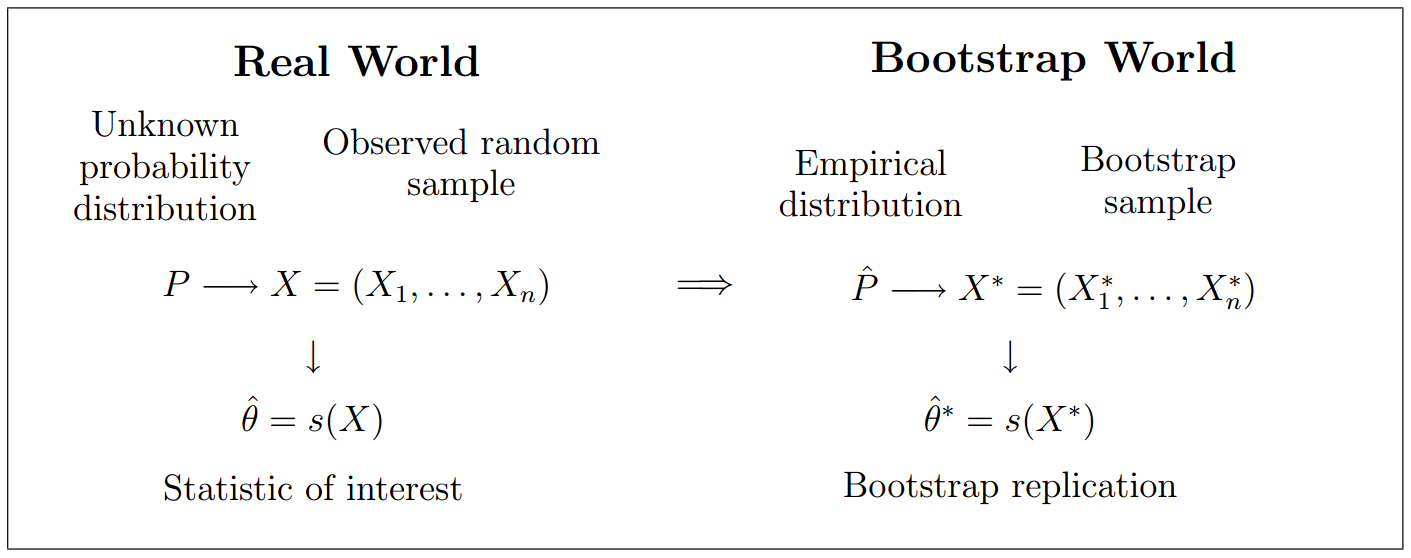
\includegraphics[width=5in]{image/bootstrap.png}
    \centering
    \caption[Bootstrapping principles]{A figure of the principles bootstrapping. Taken from~\cite{Eichler2003}}
    \label{figure:bootstrapping}
\end{figure}

\paragraph{Disadvantages}
	One prominent issue with bootstrapping is that important properties of the actual data might not be caught when undertaking the bootstrapping analysis
	~\footnote{"Bootstrapping" comes from the phrase, "to pull oneself up by one's bootstraps"~\cite{bootstrapSaying1843}}.


\paragraph{Finding the optimal parameter settings}

Finding the optimal parameters for a model is usually a crucial task in engineering approaches to classification and modeling tasks. An automated approach is particularly desirable when the number of parameters is high. In order to work well many algorithms and modeling techniques in computer science rely on a careful choice of their parameters. The usual approach is to select parameters based on some prior experience on the problem at hand with a limited heuristic search of possibly optimal parameters. When such prior knowledge is absent or cannot be directly applied to the technique being used, the optimal parameters have to be found by \emph{blind} search, by e.g. using genetic algorithms or some kind of exhaustive grid-search procedure.

The \emph{de facto} standard way of performing model selection optimization is grid search, which is simply an exhaustive searching through a manually specified subset of the hyperparameter space of a learning algorithm. To \emph{guide} the grid-search one typically uses a performance metric, typically measured by cross-validation on the training set. After evaluating the performance all the pre-specified combinations of parameter settings, the grid search algorithm outputs the setting that achieved the highest score in the validation procedure.

Many of the most popular Machine Learning libraries now come with methods for performing grid search.

\subsubsection{Offline Evaluation Metrics}

When evaluating a recommender system, you wish to estimate a user's
satisfaction for a given recommendation. Traditionally recommender systems have
been evaluated by means of predictive accuracy. However, there is now a widely
agreed that accurate predictions are crucial but insufficient to deploy a good
recommendation engine~\cite{Shani2011, McNee2006}. Some of the properties can
be traded-off, one such example is the trade-off between accuracy and
diversity. It is important to understand and evaluate these trade-offs and
their effect on the overall performance. This subsection will cover the most
popular metrics used for offline evaluation, a discussion of evaluation
measures for implicit feedback, and a summary of the cold-start evaluation
methodologies found in the literature.

\paragraph{Predictive Accuracy Metrics}

Predictive accuracy metrics measure how close the predicted ratings are to the
true user ratings. More formally, the system tries to predict ratings
$\hat{r(c,i)}$ for a test set $T$ of user-item pairs $(c, i)$ for which the
true ratings are known. Traditionally, mean absolute error (MAE) has be used to
evaluate the performance of collaborative-filtering algorithms, but other
measures such as root mean squared error (RMSE) are also commonly used.

\subparagraph{Mean Absolute Error (MAE)}

MAE measures how close the predictions are to the actual outcome.

\begin{equation}
    MAE = \frac{1}{n}\sum_{i=1}^{n}{|\hat{r(c,i)}-r(c,i)|}
    \label{equation:mae}
\end{equation}

$r(c,i)$ is the actual outcome and $\hat{r}(c,i)$ is the predicted value.
As the name suggest, $MAE$ calculates the average absolute error.

\subparagraph{Root Mean Squared Error (RMSE)}

Often used to measure difference between a set of predicted values with a set of actual values.

\begin{equation}
    MSE = \frac{1}{n}\sum_{i=1}^{n}{(\hat{r(c,i)} - r(c,i))^{2}}
    \label{equation:mse}
\end{equation}

\begin{equation}
    RMSE = \sqrt{MSE}
    \label{equation:rmse}
\end{equation}

In $MSE$~\ref{equation:mse} $\hat{r(c,i)}$ is the predicted value and $r(c,i)$ is the actual value.
Both $MAE$ and $MSE$ are used to measure how correct the predictions are compared to the actual values.
$RMSE$ is the square root of $MSE$ and is one of the most used metrics to compare recommender algorithms in collaborative filtering, and was the main metric used in the Netflix price competition to evaluate the performance of the competitors recommender systems. $RMSE$ is always bigger or equal to $MAE$, $RMSE$ penalize an error more than $MAE$.

% \todo{maybe some sweet table of the different algorithms with their eqations and their contributions}
% \begin{table}[H]
%     \centering
%     \begin{tabular}{l|l|l}
%     	% \rowstyle{\bfseries}
%     	Metric	& Equation & About \\ \toprule
%     	MEA 			& \parbox{6cm}{\equationMEA} & safd \\	\hline
%     	RMSE 			& \parbox{6cm}{\equationRMSE} & asdf \\
%     \end{tabular}
%     \label{table:predictiveAccuracyMetrics}
%     \caption [Predictive Accuracy Metrics]{adsf}
% \end{table}



\paragraph{Measuring Usage Prediction}
\label{para:measuring_usage}
% \subsubsection{Decision Based Metrics}
In many applications the recommender system does not predict the user's
preferences of items, but tries to recommend to users items that they may use.
This is often done by giving the user a top-K set of recommendations.
In an offline evaluation of usage prediction, we typically have a dataset
consisting of items each user has used. We then select a test user, hide some
of her selections, and ask the recommender to predict a set of items the user
will use. We then have four possible outcomes for the recommend and hidden
items.

\begin{table}[H]
	\centering
	\begin{tabular}{l l l}
	\toprule
					&	Relevant			&	Not Relevant \\ \midrule
	Recommended		&	True-Positive (TP) 	&	False-Positive (FP)	\\ 
	Not Recommended	&	False-Negative (FN)	&	True-Negative (TN)	\\ 
	\bottomrule
	\end{tabular}
	\label{table:usageprediction}
	\caption[Usage prediction (Confusion Matrix)]{This table is showing the different categories recommended items can end up in.}
\end{table}

\begin{table}[H]
	\centering
	\begin{tabular}{l l}
		\toprule
		True-Positive (TP)	& The recommended item is of interest to the user \\ 
		False-Positive (FP)	& The recommended item is not of interest to the user \\ 
		False-Negative (FN)	& The item is of interest to the user, but is not recommended \\ 
		True-Negative (TN)	& The item is not of interest to the user, but is not recommended \\
		\bottomrule
	\end{tabular}
	\label{table:predictionCategories}
	\caption[Prediction Categories]{}
\end{table}

This model assumes that not relevant items would not have been relevant if they had been
recommended to a user. This assumption may be false, such as when the set of
not relevant items contains some interesting items that the user did not select. For
example, a user may not have relevant an items because she was unaware of its
existence, but after the recommendation exposed that item, the user can decide
to select it. We can count the number of examples that fall into each cell in
the table and compute the Precision, Recall, Fallout and $ROC$.

\subparagraph{Precision}
Precision is the fraction of retrieved items that are relevant.
\begin{equation}
    Precision = \frac{TP}{TP+FP}
    \label{equation:precision}
\end{equation}
Precision takes all recommended items into account, but it can also be evaluated at a given cut-off point, only considering the top $n$ results returned. This measure is called precision at n or P@n.

\subparagraph{Recall}
Recall is the fraction of the items that are relevant to that are successfully recommended.
\begin{equation}
    Recall = \frac{TP}{TP+FN}
    \label{equation:recall}
\end{equation}
Recall can therefore be seen as the probability that a relevant item is retrieved by the recommender.

\subparagraph{Fallout}
Fallout is the amount of retrieved items which is not relevant amongst all the non relevant items (false positive).
\begin{equation}
    Fallout = \frac{FP}{FP+TN}
    \label{equation:fallout}
\end{equation}
Fallout can therefore be looked at as the probability that a non-relevant item is recommended.

\subparagraph{F-measure}
F-measure combines the precision and the recall.
\begin{equation}
    F_\beta = \frac{(1 + \beta^2) * (Precision * Recall)}{(\beta^2 * Precision + Recall)}
    \label{equation:f-measure}
\end{equation}
Based on the value of $\beta$ F-measure will weight precision or recall more. For a $\beta$ over 1 F-measure will emphasize precision over recall, and opposite for $\beta$ between 0 and 1.

\subparagraph{Accuracy}
Accuracy is the amount of correctly recommended items over all the items.
\begin{equation}
    Accuracy = \frac{TP+TN}{TP+TN+FP+FN}
    \label{equation:accuracy}
\end{equation}

\subparagraph{Receiver Operating Characteristics (ROC)}
The $ROC$ is the recall rate ($TPR$) against the fallout rate ($FPR$).
The goal is to maximize the recall while minimizing the fallout.
\begin{equation}
    TPR(T) = \int_T^\infty P_0(T)dT
    \label{equation:tpr}
\end{equation}
\begin{equation}
    FPR(T) = \int_T^\infty P_1(T)dT
    \label{equation:fpr}
\end{equation}
$T$ is a threshold parameter.
The ROC curve is $TPR$ plotted together with $FPR$ at various $T$.

\begin{equation}
    AUROC = \int_\infty^{-\infty} TPR(T)P_0(T)dTdT
    \label{equation:auroc}
\end{equation}
Equation~\ref{equation:auroc} can be used to calculate the area under the curve.
$AUROC$ is the probability that the recommender system will rank positive examples higher than negative examples.
The Area Under is a commonly used evaluation method for binary choice problems. If somebody makes random guesses,
the ROC curve should be a diagonal line stretching from (0,0) to (1,1), as shown by the blue line in Figure \ref{fig:aucroc}, scoring an AUC of 0.5. A perfect model will score an AUC of 1.0. In practice, almost all models will fit somewhere in between.

\begin{figure}[H]
\label{fig:aucroc}
  \centering
    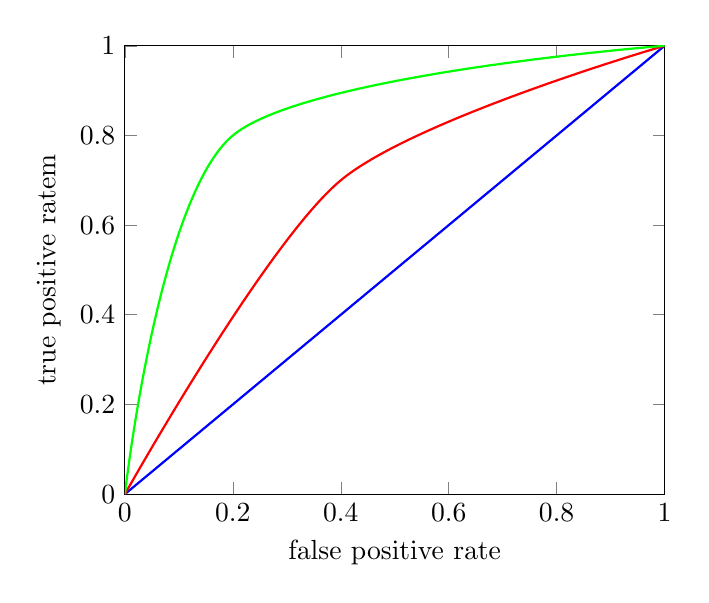
\begin{tikzpicture}
      \begin{axis}[
      	xlabel={false positive rate},
      	ylabel={true positive ratem},
      	ymin = 0, ymax=1, xmin=0, xmax=1,
      ]
      \addplot[thick,smooth,blue]{x};
      \addplot[thick,smooth,red] plot coordinates {
              (0,0)
              (0.4,0.7)
              (1,1)
          };
      \addplot[thick,smooth,green] plot coordinates {
                    (0,0)
                    (0.2,0.8)
                    (1,1)
                };
      \end{axis}
    \end{tikzpicture}
    \caption{ROC curves}
\end{figure}

\subparagraph{Limitations}
\label{subp:limitations}
As mentioned by Powers et al.~\cite{powers2007}, recall, precision, F-measure have a bias.
Recall, precision and F-measure ignore performance in correctly handling negative examples, they propagate the marginal Prevalences and biases, and they fail to take account the chance level performance.
Another drawback or limitation with the measuring of user predictions is that it does not take into account the ranking of the items. To handle this, rank based metrics can be used.

\paragraph{Rank Based Metrics}
\label{para:rank_based}
Rank accuracy metrics measure the ability of a recommendation method to produce
a recommended ordering of items that matches how the user would have ordered
the same items. Shani et al.~\cite{Shani2011} lists two different approaches
for measuring the ranking accuracy: Try determining the correct order of a set
of items for each user and measure how close a system comes to this correct
order, or we can attempt to measure the utility of the system's ranking to a
user.

Herlocker et al.~\cite{Herlocker2004} argue that rank accuracy metrics may be
overly sensitive for domains where the user just wants an item that is `good
enough' (binary preferences) since the user won't be concerned about the
ordering of items beyond the binary classification. These metrics are therefore
most suitable to evaluate algorithms that are used to present ranked lists to
the user in domains where the user preferences are expressed using numerical
values.

\subparagraph{AP correlation}
\label{subp:ap_correlation}
$AP correlation$~\cite{Yilmaz:2008:NRC:1390334.1390435} measures the overall precision and is a variant of $Kendall's$ $tau$.
It counts the amount of items correctly placed in a ordered predicted rank list $list1$ and a list of the actual rank ordering of the preferences of the user $list2$.
\begin{equation}
	AP = \frac{2}{N - 1} * \sum_{i=2}^{N}{(\frac{C(i)}{i - 1})} - 1
	\label{equation:ap}
\end{equation}
How to calculate the $AP correlation$ value is shown in ~\ref{equation:ap}.
$C(i)$ is the number of items ranked correctly above rank $i$.
The value of AP is between -1 and 1, where a score of 0 means that $list1$ can be considered a randomly generated list and 1 is a perfect match with the actual list $list2$.
% \paragraph{Limitations}
% todo maybe

\label{par:accuracy_ranking}

\marginpar{if this is the setup, write a little intro}

\subparagraph{Mean Percentage Ranking (MPR)}
\label{subp:mean_percentage_ranking_}
This measure is a recall-oriented metric.
A known issue with implicit feedback is that it often lack the actual user's preference.
This approach is used to measure the user satisfaction of items in an recommended ordered list.
\begin{equation}
	MPR = \frac{\sum_{u,i}{r_{ui} * rank_{ui}}}{\sum_{u,i}{r_{ui}}}
	\label{equation:mpr}
\end{equation}
How to calculate $MPR$ is shown in~\ref{equation:mpr}.
A list of all the items for user $u$ is ordered based on the rank $rank_{ui}$ of the $u$.
Where $rank_{ui}$ is the percentile rank of item $i$ in this list for $u$.
$rank_{ui} = 0$ means that $i$ is the most preferred item for $u$.
$r_{ui}$ indicates whether $u$ has consumed $i$ or not.
This makes a $MPR$ value of 0\% to be the most preferred value, and a value of 50\% meaning a near randomly produced list.

\subparagraph{Mean Average Precision (MAP)}

\label{subp:mean_average_precision_map_}
MAP~\cite{Manning:2008:IIR:1394399} measures quality across recall levels.

\begin{equation}
	ap@n = \sum_{k=1}^{n}{\frac{P(K)}{min(m,n)}}
	\label{equation:apn}
\end{equation}
\begin{equation}
	MAP@n = \sum_{i=1}^{N}{\frac{ap@n_i}{N}}
	\label{equation:map}
\end{equation}

How to calculate the $MAP$ value is shown in~\ref{equation:map}.
\ref{equation:apn} calculates the average precision at $n$ for a user.
From \ref{equation:apn}, $P(K)$ is the precision at $k$ in the item list, $n$ is the maximum number of predicted items and $m$ is the actual length of the predicted items list.
\ref{equation:map} calculates the mean of all the values from \ref{equation:apn}.

\subparagraph{Normalized Discounted Cumulative Gain (nDCG)}
\label{subp:normalized_discounted_cumulative_gain_}

$nDCG$ measures the graded relevance of the recommended item, the ranking quality or the usefulness of the recommended item based on its rank position.
It is often used to measure the performance of web search recommendation systems.

\begin{equation}
    DCG_k = \sum_{i=1}^{k}{\frac{2^{rel_i}-1}{log_2(i+1)}}
    \label{equation:dcg}
\end{equation}

\begin{equation}
    nDCG_k = \frac{DCG_k}{IDCG_k}
    \label{equation:ndcg}
\end{equation}

How to calculate the $nDCG$ value is shown in~\ref{equation:ndcg}.
Where $k$ is the maximum amount of suggested items, and $rel_i$ is the graded relevance of the result at position $i$.
$IDCG_k$, from~\ref{equation:ndcg}, is the ideal $DCG_k$ value.
This is the result list sorted on relevance.

\subparagraph{Half-life utility~\cite{Breese:1998:EAP:2074094.2074100}}

Assume that the further down an item is in the list the less chance there is for that item to be viewed by the user.
The rate of the decaying probability is exponential.

\begin{equation}
	HL_u = \sum_{i}{\frac{\delta(i)}{2^{\frac{i-1}{\alpha-1}}}}
\end{equation}

$\delta(i)$ is 1 if the user is interested in the item at position $i$ and 0 if not.
$\alpha$ is the viewing half-life, or half-life parameter.
The half-life utility of all the users are shown in~\ref{equation:HL}

\begin{equation}
	HL = 100 * \frac{\sum_u{HL_u}}{\sum_u{HL_u^{max}}}
	\label{equation:HL}
\end{equation}

$HL_u^{max}$ is the maximum possible value of the half-life utility value.
% \paragraph{Limitations}
% todo maybe
\marginpar{some overlapping of the algorithms (not really comparing two ranked list, but still evaluating a recommender system producing ranked lists)}

\marginpar{something like this perhaps}
% paragraph accuracy_ranking (end)


\paragraph{Beyond Accuracy}
There is an emerging understanding that good recommendations accuracy alone does not give the users of the recommender system an effective and satisfying experience \cite{Herlocker2004}. The following \emph{measures} attempts to assess a recommender systems usefulness beyond being able to provide accurate recommendations to the users.

\subparagraph{Coverage}
The term coverage can refer to several distinct properties of the system. Most
commonly, the term coverage refers to the proportion of items the
recommendation system can recommend, also known as \emph{item-space coverage}.
The simplest measure of catalog coverage is the percentage of all items that
can ever be recommended. Coverage can also be the proportion of users
interactions for which the system can recommend items, known as
\emph{user-space coverage}. In many applications the recommender system may not
provide recommendations for some users due to e.g.\\ low confidence in the
accuracy of predictions for that user. In such cases one may prefer a
recommender that can provide recommendations to a wider range of users. However, an increase in coverage is only beneficial if the accuracy does not drop significantly.

\subparagraph{Perceived quality}
To gather the perceived quality the system must ask the user to examine the recommended item, and give feedback regarding the their actual interest in the recommended item.
For the feedback from the user to be as complete as possible, the system must supply the user with the reason to why the item was suggested, and the metadata of the item.
When the user has this overview of the item, the user's feedback regarding the item can produce some quality measure.
One  way of having the user to give this feedback is to re-rate the recommended item on a similar scale as the item was rated.
A rating scale from 1 to 5 is often used for both~\cite{Schafer:1999:RSE:336992.337035}.

\subparagraph{Novelty and Serendipity}
Some recommender systems produce highly accurate recommendations and also have reasonable coverage - and yet that are useless for practical purposes. For instance, a music recommender can recommend Rihanna to every customer who have not yet listened to Rihanna. However, statistically, this is highly accurate as most people have listened to Rihanna or at least knows about her and have consciously chosen not to listen to her. Much more valuable would be a recommendation to a kick-ass indie-rock band that the active user would love, but will never hear about in the news. We therefore need a new dimension for analyzing recommender systems that consider "nonobviousness" of the recommendations. One such dimension is \emph{novelty}. Another related dimension is \emph{serendipity}. A serendipitous recommendation helps a user find a surprisingly interesting item the user might not have discovered otherwise. To clarify the difference between the two, a novel recommendation could be to recommend an unknown album from one of the users favorite artists, that the user likely eventually would have discovered herself. However, a recommendation by an unknown artist is more likely to be serendipitous. Serendipity is therefore a measure of how surprisingly the successful recommendations are.

As novelty is the the degree of new and interesting items recommended for the user, the system must ask the user for feedback to be able to make any assumptions around the novelty.
The novelty together with perceived quality allows the system to make informed decisions about the ratio of new items to recommend for the user.
The novelty is expected to change over time, some times the user would like to receive recommendation on new items, and other times recommendations closer to the user's preferences.
For the system to be able to detect these changes in preferences, and acting accordingly would be beneficial in regards of the user's satisfaction.
\begin{equation}
    Novelty(u) = \frac{1}{N}\sum_{i=1}^{N}{1 - Knows(u,i)}
    \label{equation:novelty}
\end{equation}
In~\ref{equation:novelty} $Knows(u,i)$ represents a binary functions which returns 1 if the user $u$ knows the item $i$, and 0 if not.
The set of items used for the calculation is the set of recommended items for the user.

The system should be able to produce items both items known to the user, and items unknown to the user.
For trust in the system and novelty respectively.

\begin{figure}[H]
    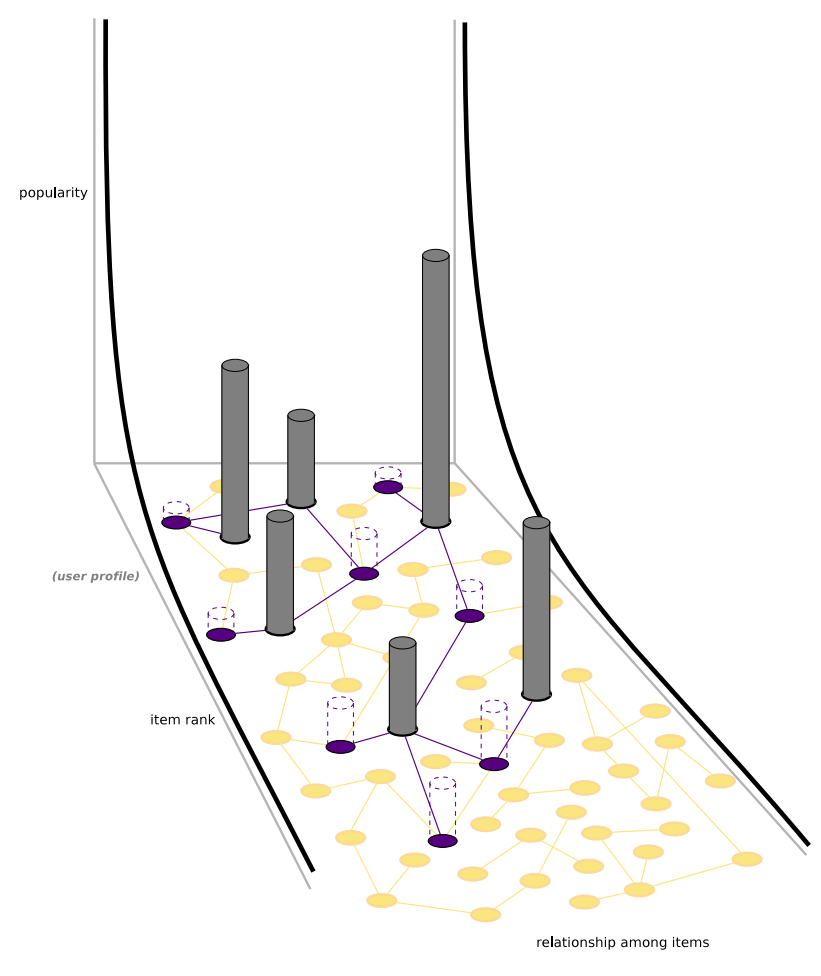
\includegraphics[width=5in]{image/longtailNoveltyFig.png}
    \centering
    \caption[Long tail]{Long tail show with the item similarity between items. Similarity shown though edges between the nodes. The gray columns represents the user profile, the violet represents items which might be of interest to the user, and the height is the relevance. Adapted from~\cite{celma2008}}
    \label{figure:longtailNovelty}
\end{figure}
\marginpar{todo - not sure if its ok to use this image (not self made) figure from music recommendation, but long tail applies to fashion}
\marginpar{todo - if so, something about longtail}

\subparagraph{Diversity}
Diversity is generally defined as the opposite of similarity. In some cases suggesting a set of similar items may not be as useful for the user, because it may take longer to explore the range of products. E.g. when presenting a list of 5 recommendations, the system should not recommend 5 Ralph Lauren shirts with different colors. As diversity may come at the expense of other properties such as accuracy, one should evaluate the decrease in accuracy vs. the increase in diversity.

Other evaluation methods worth knowing about includes confidence, trust, utility, robustness, adaptivity, scalability mentioned in \cite{Herlocker2004, Shani2011}.

\subparagraph{User-Centric Evaluation}
User-centric evaluation focuses on the perceived quality of the recommendation system~\cite{Pu:2011:UEF:2043932.2043962,Knijnenburg:2011:PPS:2043932.2043993}.
To gather this kind of information, user feedback is required.
User-centric evaluation is meant to handle the short comings of the offline evaluation metrics, such as predictive accuracy metrics.
User-centric evaluation can make evaluations on items which the user has not yet show interest in.
This allows user-centric evaluation to make evaluations on information about the system, such as the perceived quality and novelty of the recommendation system.
When the user feedback has been gathered the data must be analyzed.

\marginpar{move offline beyond accuracy to here maybe? }


\subsubsection{Evaluation using Implicit Feedback}
Accuracy metrics such as RMSE and MAE are not especially well suited for implicit feedback datasets, as they require knowing which items are undesired by a user~\cite{Hu2008}.
One way to handle the issue with missing negative feedback is through conversion of the implicit feedback to explicit feedback, and thereby producing a sense of negative feedback.
One issue with this is what is considered as negative feedback in the sense of implicit feedback.
The reason for a user not to access an item is not necessarily grounded in dislike, but could simply be an overlook.
On the other hand, if the user accessed the item for a short time without buying it, the user might not like it.
These questions raises the need for a different approach when wanting to measure a recommender system using implicit feedback.

Joachims et al.~\cite{Joachims07evaluatingthe} shows that clicks can be biased, and has to be interpreted relative to the order of presentation and relative to the other abstracts.

\marginpar{extend}

Two ways of measuring the system is through ranking and usage prediction described earlier.

\paragraph{Rank Based} % (fold)
	\label{par:Ranking_based}
	The ranking approach can be considered more suited to test recommendation systems using implicit feedback since a subset of the items are meant to be recommended to the user.
	This subset is usually a ranked top K list of items where the items in this list is the items the system predicts will be most liked by the user.

	One issue with this approach is that the items in the predicted top K list has to be ranked in some way, the same goes for the list this list is to be compared to.
	Thereby producing the requirement for a ranked list of preferred items from the user.
	If there is such a ranked list, ranking accuracy will help to tell how well the system is suggesting items for the user, such as~\cite{Yilmaz:2008:NRC:1390334.1390435}.
% paragraph paragraph_name (end)

\marginpar{maybe hard to differentiate between the names}

\paragraph{Accuracy Ranking} % (fold)
	\marginpar{HELGE: Språk!}
	\label{par:usage_prediction}
	When there is lack of explicit user feedback and a ranked list of the items cannot be produced, ranking the predicted list and scoring this list based on the actual user preferences can be used to evaluate the system.
	The actual user preferences are a list of binary preferences for the items.
	This list is often possible to construct from implicit feedback, but will seldom be a complete list, and most often be a list with only positives (not possible to produce not interesting).
	Some of the different approaches when dealing with implicit feedback are:
	Li et al.~\cite{deLace2010} who used $MPR$ and $MAP$ to calculate their performance.
	Pan et al.~\cite{Pan:2013:GGP:2540128.2540516} who used a set of top-k evaluation metrics: precision, recall, F1, nDCG, ROC and 1-call.
	Sindhwani et al.~\cite{Sindhwani:2010:OMC:1933307.1934641} who used roc curve and precision-recall curve to evaluate their experiments.
	Pan et al.~\cite{pan2008} who used $MAP$ and Half-life Utility.

	$nDCG$, $MAP$ and Half-life utility has a similar setup.
	They all have a decaying factor, and rewards the system in different ways for how high in the list a relevant recommended item is.

	On the other hand metrics as Precision alone has no decaying factor, and will not penalize a system with uninteresting items suggested higher in a ranked list.

	% \cite{Nati03weightedlow-rank} average squared difference
% paragraph usage_prediction (end)

	%TODO - What evaluation measures are suited for implicit feedback, and why are traditional evaluation measures such as RMSE, ... not as suitable when working with implicit feedback?

\subsubsection{Evaluation of Cold-start Recommendations}
\label{sec:cold-start-eval}
\marginpar{Helge: Pros og Cons plz}
\marginpar{Fix pros pg cons, for mye "synsing}

The cold-start problem can be considered a sub problem of coverage. The cold-start
problem occurs when the recommender system cannot draw any inferences for user or items
which it has not yet gathered sufficient information. When
evaluating the cold-start system performance one is interested in measuring the
system accuracy for these users and items.

The evaluation metric used depends on the type of feedback available.
Most experiments carried out have used \emph{traditional} explicit feedback datasets such as
MovieLens, EachMovie, Netflix etc. Accuracy metrics such as MAE~\cite{Rashid2002, Rashid2008, Massa2004,
Massa2007, Stern2009} and RMSE~\cite{Agarwal2009, Agarwal2010} are therefore
the most used ones. In the experiments where binary rating data have been used
Precision@N~\cite{Liu2011, Gantner2010}, ROC curves~\cite{Agarwal2009,
Gantner2010, Schein2002} and Area Under Curve (AUC) \cite{Liu2011, Gantner2010} seems to be the
preferred evaluation metrics.

Another way to discriminate between different recommender techniques is
coverage. The recommender system may not be able to make predictions for every
item. For this reason, it is important to measure the portion of ratings that
an RS is able to predict (ratings coverage). However, this quantity is not
always informative about the quality of a recommender system. A RS is likely to
be good at predicting nearly all the ratings for heavy users and not be able to
do the same for users who have rated few items. For this reason, one should
also compute the users coverage, defined as the portion of users which the RS
is able to predict at least one rating for. Good et al.~\cite{Good1999}
measure the item-space coverage, while Massa et al.~\cite{Massa2004,
Massa2007} measures both the item-space coverage and user-space coverage of
their methods.

Massa et.\ al~\cite{Massa2004} argue that performance measures such as Mean
Absolute User Error (MAUE) is a good measure for cold-start recommendations
since every user is taken into account once and a cold start user is as
influential as an heavy rater. Similarly, Park et al.~\cite{Park2006} measure
normalized MAE (NMAE) by macro-averaging, which first calculates the mean
average error of each users and taking the average of all users.

To simulate the cold-start scenario, different approaches have been employed:
One popular way to simulate a cold-start user scenario used by~\cite{Stern2009,
Lam2008} is to split the dataset in two disjoint sets, a training set
containing 90\% of the users and the remaining 10\% being in the test set. For
each test user one trains a model with a random subset $T\%$ of their ratings
e.g.\ $5\%$ or $75\%$, and then use the model to predict their remaining
ratings. The same methodology can also be used to simulate a cold-start item
scenario. Another highly similar way to simulate the cold-start user and
cold-start item scenario was used in~\cite{Rashid2002, Rashid2008}. For the
cold-start user scenario one selects a subset of the users with e.g.\ more than
200 ratings. One then trains the model with a subset of the ratings. In the
case of~\cite{Rashid2002} 30, 45, 60 and 90 ratings was used. After training
the model one computes the error on the hidden ratings for the same user.
Stern et. al. \cite{Stern1998} also used a similar method which they called Given $n$, in which
they trained their model using 2, 5 and 10 ratings for each test user and predict
the remaining values.

%Pros & Cons
The advantage of the latter approach is that they use a selection criteria for the test users
to avoid users with really few ratings which might be crucial on a cold-start dataset.
The obvious problem with this approach is that for cold-start datasets these users might stand for a large portion of the ratings. There are both pros and cons of using a fixed subset of ratings rather than using the percentage of ratings, the best choice will most likely depend on the dataset. Using a fixed subset of ratings would be preferable e.g. if the number number of ratings given by the users are fairly uniform.

Another \emph{simpler} approach employed by~\cite{Massa2007, Jamali2009} is to
determine a cutoff point for what is considered a cold-start user. E.g.\ that
every user with less than 5 ratings is considered a cold-start user. Then
separately measure the error on predictions made to these users.

%Pros & Cons
The problem with this approach is that it does not measure how well the recommendation quality improves as
users provide an increasing amount of ratings, giving a less detailed view of the systems performance.
The number of ratings predicted is also likely to be fairly small given a cold-start dataset.

To simulate a cold-start system scenario Agarwal et al.~\cite{Agarwal2009}
split the dataset in two using 75\% of the dataset for training and 25\% for
testing. They then train the model using 30\%, 60\% and 75\% of the data and
compare their performance on the testset.

%Pros & Cons
Good and simple model as it is likely to generate three different training sets
with different sparsity levels, which is exactly what we want to test. However,
if the training examples are drawn at random the experiment should be repeated multiple
times to avoid getting \emph{unfortunate} splits.


%Summary of articles read

%	What evaluation metrics are used?

%\cite{Rashid2008}: Accuracy metric: MAE, Expected Utility (Penalize false positives more than false negatives)
%\cite{Rashid2002}: Accuracy metric: MAE
%\cite{Massa2004}: Leave one out, MAE, MAUE, Rating Coverage, User Coverage
%\cite{Massa2007}: Leave one out, MAE, MAUE, Rating Coverage, User Coverage,
%\cite{Jamali2009}: Leave one out, Recall/Hit-ratio
%\cite{Agarwal2009}: Movie: RMSE, Yahoo: ROC curves, 5-fold cross validation
%\cite{Agarwal2010}: RMSE, True Positive Rate, True Positive Rate
%\cite{Liu2011}: Precision at N, Mean average precision, area under curve
%\cite{Park2006}: NMAE
%\cite{Good1999}: Coverage, MAE, ROC
%\cite{Stern2009}: MAE
%\cite{Ganter2010}: Precision at N (5 & 10), AUC (General ranking measure)
%\cite{Schein2002}: GROC (hit/miss rate)

%	What type of user feedback is used?

%\cite{Rashid2008}: Explicit feedback, MOVIELENS, Only users with 80 or more ratings
%\cite{Rashid2002}: Explicit feedback, MOVIELENS, Only users with 200 or more ratings
%\cite{Massa2004}: Explicit feedback, EPINIONS + Web of trust
%\cite{Massa2007}: Explicit feedback, EPINIONS + Web of trust
%\cite{Jamali2009}: Explicit feedback, EPINIONS + Web of trust
%\cite{Agarwal2009}: Explicit feedback, MovieLens + EachMovie, also incorporates user features
%\cite{Agarwal2010}: Explicit feedback + User features and bag of words rep of crawled movie data - MovieLens, Yahoo! Buzz (1 or -1), BookCrossing
%\cite{Liu2011}: Explicit feedback. Netflix...
%\cite{Park2006}: Explicit feedback, Yahoo!, MovieLens, EachMovie
%\cite{Stern2009}: MovieLens, Netflix,
%\cite{Ganter2010}: MovieLens - Binary (likes, not likes)
%\cite{Schein2002}: MovieLens, Movielens(Stripped of ratings -> implicit)

%	How do they similate the "cold-start situation"?

%\cite{Rashid2008}: Use the movies found when presenting 15, 30, 45, 60, 75 movies to provide predictions for the remaining movies in the list of each user
%\cite{Rashid2002}: Use the movies found when presenting 30, 45, 60, 90 movies to provide predictions for the remaining movies in the list of each user
%\cite{Massa2004}: Consider users who provided 2, 3 or 4 ratings, How does trust propagation of 1,2,3,4 affect rating & user coverage and predictive accurracy?
%\cite{Massa2007}: All users, cold users, heavy users, Controversial items, Black sheep, Trust propagation performance on entire dataset
%\cite{Jamali2009}: All users, cold start users (<5 ratings), recall for different neighborhood sizes
%\cite{Agarwal2009}: 25\% set aside for evaluation, train each model with 30\%, 60\%, 75\% of data, compare performance
%\cite{Agarwal2010}:
%\cite{Liu2011}: User cold start: Split users into disjoint sets (training, test). Item cold start: Split into disjoint sets
%\cite{Park2006}: Fraction of training data used [0.1 -> 1.0]. Cold-start user: Select users with more than 40 ratings in the training set and more than 1 in the test set. Split into 5, with 20\% of the users in each training set. Starting at 2 ratings, add 2 additional training set ratings per iteration until 40 ratings are added. Take the average of the 5 to compute the NMAE. Cold-start item: Items rated by more than 40 users in training data, and at least 1 user in test set. Split in 5. Starting from 2, add 2 more users per iteration. Take average NMAE from each split.
%\cite{Stern2009, Lam2008}: Divide users in two sets (90:10), train model on the 90\%. For each test user train the model on a random subset of T\% of their ratings for T = 5, T=75, then use the model to predict the remaining ratings for the user

%Clues
% http://delivery.acm.org/10.1145/570000/564421/p253-schein.pdf?ip=129.241.103.83&id=564421&acc=ACTIVE%20SERVICE&key=CDADA77FFDD8BE08%2E5386D6A7D247483C%2E4D4702B0C3E38B35%2E4D4702B0C3E38B35&CFID=419807217&CFTOKEN=62708098&__acm__=1394537427_86c608d0d7733db023faa5a09da46de7

\subsection{Online Evaluation}

Instead of doing offline evaluations on the system, one could also run large
scale experiments on a deployed system. Such experiments evaluate the
performance of recommender systems on real users which are oblivious to the
conducted experiment. The real effect of a recommender system depends on a
variety of factors such as user’s intent, the user’s context and how the
recommendations are presented to the user. All these factors are hard to
capture in an offline setting. Thus, the experiment that provides the strongest
evidence as to the true real value of the system is an online evaluation, where
the system is used by real users to perform real tasks.

\subsubsection{Online Evaluation Metrics}

Online studies in recommendations and advertisement usually measure the
click-through-rate (CTR) of the recommendations, which aligns with financial
incentives and implicitly factors in accuracy, novelty, diversity, etc.,
according to the preferences of the distribution of users.  The
click-through-rate of an algorithm is defined as the number of clicks your
recommendations get divided by the total number of recommendations that have
been made. A high CTR therefore indicates that your system is doing well.

\begin{equation}
CTR = \frac{Clicks}{Recommendations}
\end{equation}

\subsubsection{A/B Testing}
	A/B testing or bucket testing is used to test a system on live audience.
	In its' simplest form the audience is split into two groups, but it is also possible to make multiple groups of users.
	The different groups are presented with different altered versions of the system and is asked to use the system as they normally would.
	The goal is to figure out which version is producing the best results, whether it is user satisfaction or revenue.
	How the altered versions are scored is usually done trough a measure of the applications main goal, for instance with an e-commerce application where the main goal is to sell items, the score could be revenue produced by that version.

\paragraph{Example}
	In the case with the SoBazaar application, on way of doing a A/B testing on the system is as follows:
	3 groups of users are made, one with the unaltered system, one with method $A$ to produce recommendations and one with method $B$.

\subparagraph{Group Split} % (fold)
\label{par:group_split}
	The groups of users can either be selected to fit the global distribution of users, or be a set of similar minded users.
	The latter case might benefit a system where the intended goal is to specialize the system for a set of users, or actually partition the system into fitting a subsets of its' users.

\subparagraph{Group Size} % (fold)
  \label{par:group_size}
	The size of the groups depends on the amount of splits and intended stability of the system.
	The group with the original system will be the biggest group to maintain the established image of the application.
	For a system with a well established image, and a large set of faithful users, changes in the system might produce unwanted results.
	The two groups with the altered versions of the system can be of the same size to make it simpler to measure the performance of the two system against one another.

\subparagraph{System Measuring} % (fold)
\label{par:system_measuring}
	After a set period of time, the two altered versions are compared to one another and the original system.
	This is done trough measuring either the revenue produced or clicks.
	For a recommender system it is not just interesting to look at the final income number, but also if the user actually showed any interest in the products recommended for the users.
	If a larger portions of the users from version $A$ showed an increased interest in the recommended items compared to the users from version $B$, that might indicate that version $A$ is a stronger system than system $B$

\paragraph{Disadvantages}
	An issue with A/B testing is that when splitting the users into subgroups of users, these subgroups might not possess the same user properties as the complete set of groups had.
	This might lead to a biased score for the group, which might not reflect the actual score of the system when releasing it on the full set of user groups.


\subsubsection{Multi-armed bandit experiments \cite{googlebandit}}
	
	A multi-armed bandit is a type of experiment where:
	
	\begin{itemize}
	\item The goal is to find the best or most profitable action
	\item The randomization distribution can be updated as the experiment progresses
	\end{itemize}
	
	The "multi-armed bandit" described a hypothetical example where you face several slot machines ("one-armed bandits")
	with potentially different payouts. You wish to find the slot machine with the best payout rate, but you also want to
	maximize your winnings. The fundamental tension is between "exploiting" arms that have performed well in the past
	and "exploring" new or seemingly inferior arms in case they might perform better. 
	
	In normal A/B testing, you will split the traffic equally between both systems, meaning that both get 50\% of the
	traffic each, all the time. When using bandits you can continuously adjust the traffic each variation receives based on its
	performance. Variations that appear to do well gets more traffic, and variations that clearly is underperforming
	gets less. The adjustments are made based on a statistical test that considers both the sample size and performance
	metrics together.
	
	\paragraph{Advantages}
	
	The main advantage of using multi-armed bandit experiments is that it usually performs better than A/B testing
	when we look at average conversion rates, which in turn will decrease the cost of the experiment.
	Saved testing time is another advantage highlighted in the Google article.
		
	\paragraph{Disadvantages}
	
	Statistical significance. Instead of sending equal traffic to each of the test pages, the page which performs
	better will start to get more traffic. If you are running tests across pages which do not get huge amounts of
	traffic, one variant can run away while the others are left in the dust without getting a fair chance. Of course,
	if your variation is performing badly you will loose some sales or conversions in the process of A/B testing,
	but that is the price one have to pay for finding out if a variation really did perform badly.

\subsection{Discussion}
The main idea behind a recommendation system is to produce a set of items which are of interest to the user.
For the system to be successful, this sets of items needs quality.
But what needs to be considered when determining the quality of the recommendations?
According to a user study~\cite{Pu:2011:UEF:2043932.2043962} the most central aspects to this quality is:

% \todo{as list or in table, or not}

\subsubsection{Perceived accuracy}
The degree of how well the user perceives the recommended items match the actual want of the user.

\subsubsection{Novelty}
The degree of new and interesting items recommended for the user.

\subsubsection{Attractiveness}
How well the recommended items are able to evoke interest or desire in the user.

\subsubsection{Diversity}
How different the recommended items are.

\subsubsection{Context compatibility}
How the system uses contextual factors to supply the recommendations with more personalized recommendations.


\subsection{The Good}
Since the data at hand is mainly implicit feedback and this data is sparse, some natural ways of approaching the evaluations task would be:

\subsubsection{MPR}
\begin{itemize}
	\item good
	\item Possible to produce a score for a recommender system which relies on implicit feedback
	\item Usable even though there are no feedback indicating undesired items
	\item Does not need a ranked list of the actual preferences of the user
	\item bad
	\item Needs distinct ranking of the different items
\end{itemize}

\subsubsection{MAP}
\begin{itemize}
	\item good
	\item Possible to produce a score for a recommender system which relies on implicit feedback
	\item Usable even though there are no feedback indicating undesired items
	\item Does not need a ranked list of the actual preferences of the user
	\item Differentiates between predicted more desired items and those that are not
	\item bad
	\item Needs distinct ranking of the different items
\end{itemize}


\subsection{The Bad}
\subsubsection{RMSE}
\begin{itemize}
	\item good
	\item Well known, so it produces a clear score of the system
	\item bad
	\item Needs the actual rating of the items
	\item Needs a predicted rating for the items
	\item Not easy to gather reliable information about undesired items trough implicit feedback
\end{itemize}



% !TEX root = ../report.tex

\chapter{Algorithmic background}
\label{chap:algbackground}
\minitoc

This chapter will present:
- The recommendation algorithms used in our experiments.
- Cold start solutions

\clearpage

% !TEX root = ../../report.tex

\section{Common recommender algorithms}

%Having a large amount of data like e.g. in the netflix dataset
% -> Do not require a great understanding of the data to get decent results
% -> Out case is a little different. What implications does the limited amount of data have?

%We need to take this into account when designing our system / selecting methods for recomendations


\subsection{Some Awesome Algorithms (Build up with project progress)}

This section aims to describe the algorithms which will be evaluated in our experiment.

\subsubsection{Most-popular Recommender}

We have developed a simple most-popular recommender that uses result dithering to \emph{randomize} the recommendations to the users. One could imagine to final system to leverage multiple recommendation techniques. When users are new to the system they are recommended the most popular items, until enough data is collected to provide personalized recommendations. One could imagine multiple categories of most popular recommendations: Most viewed, most wanted, most bought or a combination of all.

Dithering adds \emph{noise} to the algorithm, which permutes the results in such a way that the top few results have a high probability of remaining on the top spots, but as one goes deeper into the results, the degree of mixing increases dramatically. It is important to note that dithering is \emph{guaranteed} to make off-line performance worse, but is likely to make the actual performance better. We have experimented with two different methods of dithering:

\begin{itemize}
\item Score = log2(rank+x) - runif(y, z)
\item Score = log2(rank+x) - y*rexp(z)
\end{itemize}

Given $x=1$, $y=8$ and $z=2$ alternative one generated the following permutations of the original ranking in 10 runs:

\begin{table}[H]
	\centering
	\begin{tabular}{*{11}l}
	\toprule
	\multicolumn{1}{l}{\#Run} & \multicolumn{10}{l}{Result} \\ \midrule
	1 	& 8 & 3 &  24 &  20 &  1 &  19 &  22 &  15 &  42 &  36 \\
	2 	& 2 &  0 &  1 &  32 &  20 &  3 &  35 &  34 &  43 &  10 \\
	3	& 7 &  1 &  3 &  12 &  2 &  25 &  0 &  9 &  24 &  27\\
	4	& 0 &  4 &  3 &  5 &  7 &  16 &  26 &  22 &  13 &  33\\
	5	& 0 &  10 &  8 &  1 &  15 &  5 &  30 &  17 &  11 &  35\\
	6	& 7 &  4 &  6 &  12 &  2 &  1 &  19 &  0 &  27 &  9\\
	7	& 1 &  5 &  0 &  2 &  9 &  3 &  20 &  12 &  4 &  31\\
	8	& 0 &  1 &  2 &  5 &  39 &  4 &  15 &  41 &  10 &  22\\
	9	& 4 &  6 &  0 &  3 &  1 &  29 &  36 &  31 &  35 &  20\\
	10	& 5 &  1 &  0 &  8 &  3 &  18 &  25 & 24 & 2 & 28\\
	\bottomrule
\end{tabular}
\end{table}

Given $x=1$, $y=3.0$ and $z=2.5$ alternative two generates the following permutations of the original most popular ranking in 10 runs:

\begin{table}[H]
	\centering
	\begin{tabular}{*{11}l}
	\toprule
	\multicolumn{1}{l}{\#Run} & \multicolumn{10}{l}{Result} \\ \midrule
	1& 2 &  4 &  0 &  35 &  3 &  1 &  15 &  72 &  9 &  5\\
	2& 0 &  10 &  11 &  17 &  1 &  3 &  8 &  41 &  15 &  5\\
	3 & 44 &  1 &  0 &  15 &  9 &  4 &  5 &  59 &  26 &  2\\
	4& 0 &  98 &  1 &  4 &  2 &  41 &  8 &  26 &  11 &  94\\
	5& 0 &  6 &  1 &  2 &  70 &  4 &  19 &  14 &  8 &  3\\
	6& 2 &  5 &  0 &  16 &  15 &  18 &  1 &  3 &  32 &  6\\
	7& 2 &  65 &  4 &  0 &  3 &  45 &  8 &  1 &  48 &  36\\
	8& 3 &  49 &  5 &  0 &  2 &  82 &  8 &  77 &  11 &  4\\
	9& 0 &  1 &  21 &  8 &  4 &  85 &  2 &  6 &  47 &  3\\
	10& 0 &  1 &  21 &  70 &  11 &  20 &  2 & 10 & 9& 3 \\
	\bottomrule
\end{tabular}
\end{table}

Here 0 is the most popular item before the permutation. The results show that alternative two has a higher degree of mixing than alternative one, as the added noise is larger than alternative one. The values of $x$, $y$ and $z$ can be modified to achieve the desired degree/level/amount of mixing.

\subsubsection{Item-Average}

Item average is a simple recommender that always estimates the preference for an item to be the average of all known preference values for that item. No information about users is taken into account. This recommender can therefore be considered a \emph{highest rated} recommender, as it is likely to recommend the highest rated items. The following equation shows the rating prediction procedure:

\begin{equation}
\label{equation:itemaverageratingprediction}
u(c,s) = k * \sum_{c' \epsilon C} u(c',s)
\end{equation}

Where $k$ again is a normalization factor ($1/|C|$). This is somewhat similar to collaborative filtering, except for the fact that the user similarity $sim(c, c')$ has been taken out of the equation. It is also worth mentioning that this method is not suited for binary ratings, as the result is likely to be very random, and should therefore not be used without item ratings to average.

\subsubsection{User-based Collaborative Filtering}

Recommend items by finding similar users. This is often harder to scale because of the dynamic nature of users. The pearson correlation coefficient is used to calculate the user similarities. For a more in depth description of user-based collaborative filtering see Section \ref{subsec:cf}.

\subsubsection{Item-based Collaborative Filtering}

Calculate similarity between items and make recommendations. Items usually don't change much, so this often can be computed offline. For a more in depth description of item-based collaborative filtering see Section \ref{subsec:cf}.%

\subsubsection{ALS-WR}

Alternating-least-squares with weighted-$\lambda$-regularization (ALS-WR) was designed fro the Netflix Prize Competition \cite{Netflix}, where it obtained an RMSE score of 0.8975, which was one of the best results based on a pure method.

Alternating-least-squares is a method to solve Equation \ref{equation:minimize}. Since both $q_{s}$ and $p_{c}$ are unknown, the equation is not convex. However if we fix one of the unknowns, the optimization problem becomes quadratic and can be solved optimally. The ALS technique rotate between fixing the $q_{s}$'s and fixing the $p_{c}$'s. When all the $p_{c}$'s are fixed, the system recomputes the $q_{s}$'s by solving a least-squares problem, and vica versa. This ensures that each step decreases the error until convergence. What makes ALS favorable over the simpler and faster stochastic gradient descent is two things. ALS can be parallelized since the system computes the $q_{s}$'s independently of the other item factors, the same can also be applied to the user factors. The second case if for systems centered around implicit data. Because the training set cannot be considered sparse, looping over each single training case as gradient descent would not be practical, but ALS can efficiently handle such cases \cite{Hu2008}.\newline

ALS solves the low-rank matrix factorization as follows:

\begin{itemize}
\item Step 1: Initialize the matrix M by assigning the average rating for that movie as the first row, and a small random numbers for the remaining entries;
\item Step 2: Fix P, solve Q by minimizing the objective function (the sum of squared errors);
\item Step 3: Fix Q, solve by minimizing the objective function similarly;
\item Step 4: Repeat Steps 2 and 3 until a stopping criterion is satisfied.
\end{itemize}

Zhou et. al. \cite{Zhou2008} used the difference in RMSEs between the rounds as a stopping criterion. Without regularization ALS might lead to overfitting due to the many free parameters. Regularization was therefore introduced in the form of weighted-$\lambda$-regularization to prevent the model from overfitting.

\begin{equation}
f(P, Q) = \sum_{(c,s)\epsilon C} (u(c,s) - p^{T}_{c}q_{s})^{2} + \lambda (\sum_{c} n_{p_{c}} \Vert p_{c} \Vert ^{2} + \sum_{s} n_{q_{s}} \Vert q_{s} \Vert ^{2})
\label{WeightedLamba}
\end{equation}

where $n_{p_{c}}$ and $n_{q_{s}}$ denote the number of ratings of user $c$ and item $s$ respectively. $S_{c}$ denote the set of items $s$ that user $c$ rated, then $n_{p_{c}}$ is the cardinality of $S_{c}$; similarly $C_{s}$ denotes the set of users who rated item $s$, and $n_{q_{s}}$ is the cardinality of $I_{s}$. A given column of P, $p_{c}$ is found by solving a regularized linear least squares problem involving the known ratings of user $c$, and the feature vectors $q_{s}$ of the items that user $c$ has rated. Similarly, we can compute individual $q_{s}$'s via a regularized linear least squares solution, using the feature vectors of users who rated item $j$, and their ratings of it.

\subsubsection{Content-based}

To build features we had to take a closer look at the content in the product database. To find the product-type, material, style and color we looked at the title, description and meta-description fields looking for certain keywords. The fact that descriptions could be either in Norwegian and in English we had to include the words from both languages in the check. To find the words to classify the items we looked through the top keyword lists in both languages, and tried to group them manually as logical as possible. E.g. to determine if a product falls under the \emph{sweater} category we check for the following keywords: \emph{sweater, cardigan, jumper, hoody , genser and genseren}. As you can see we included the same word but with different suffixes. We experimented with stemming from the nltk software package in python, but we did not feel that it improved
our results, we therefore decided to not use stemming. We attempt to extract the following features from the product-database content: brand or storename which is easily collected as it is stored in its own unique field, the price which we grouped into price brackets, the product-type such as e.g dress, jacket, top, pants boots, the product-material such as e.g. cotton, wool polyester etc., the style or genre of an item, and lastly the color of an item. 

It was a pleasant surprise to find out that 3,263 out of 3,386 items could be found in the
product database and be assigned features. The following table shows an overview over how many items we were able to extract the different features for.

\begin{table}[H]
	\centering
	\begin{tabular}{l l}
	\toprule
	Attribute & Percentage \\ \midrule
	Price 			& 1.000 \\ 
	Brand 			& 0.756 \\ 
	Product-type 	& 0.625 \\ 
	Material 		& 0.44  \\ 
	Style 			& 0.234 \\ 
	Color 			& 0.203
	\\ \bottomrule
	\end{tabular}
\end{table}

As you can see the price, brand and product-type can be found for \emph{most} items, while material style and color could only be found for a minority of the items.

%Problems? Limited amount of features\documentclass[options]{class}
%Table with features?

\subsection{Cold-start Solutions}

%Justify why we only tested out one approach...

The number of cold-start solutions we are currently able to test out is pretty limited.

As we never got access to more than item-features, we can cross out RBLF and others
methods that require user features in addition to item-features. This leaves us with
Naive Filterbots \cite{Park2006} which easily could be combined with our implicit ratings.

\subsubsection{Filterbots}

As one simple solution to the cold-start problem we decided to experiment with Filterbots, as it easily
combined with our implicit ratings. Similarly as in \cite{Park2006} we decided to experiment with global bots.
We implemented the following filterbots: A \emph{BrandBot} which rates an item based on the brands average rating, an \emph{AverageBot} which rates an item based on their average rating given to it, a \emph{CriticBot} which selects $n$ critics among the most active users and rate items based on their average rating, a \emph{PopularityBot} which rates an item based on its popularity, more ratings equals a higher rating.


Each bot is added as a single user into our training set. It is also worth noting that we use the training set only (obviously) to generate the bot ratings. Filterbots can potentially help solve the cold-start user problem by making it possible for new users to connect to users that capture the general underlying trends of the entire user group. Filterbots are mainly meant to improve performance when data is scarce and not to degrade performance when data is plentiful.

\marginpar{TODO: Write in incorporation of recency and similar in our filterbots}
\marginpar{Incorporating recency in filterbots}

%E.g. most popular recommender, only look at most popular items for the last week (used to give recommendations to new users)
%Item-average: Only include items rated the last 2-3 months


%\subsection{Some one-class collaborative filtering...}

\subsubsection{The Good}
\subsubsection{The Bad}
\subsection{Why Not To Use These (Same As above)}
\subsubsection{The Good}
\subsubsection{The Bad}


% !TEX root = ../report.tex

\chapter{Implementation}
\label{chap:implementaion}
\minitoc

\clearpage

% !TEX root = ../../report.tex

\section{Generating implicit ratings}
\label{implementation-implicit}

In this section we continue solving the problem of generating ratings based on
implicit feedback found in analytics logs, as defined in
Section~\ref{implicit-feedback}. Our goal is two-fold:

\begin{itemize}
  \item Find novel ways of creating implicit ratings, remedying as many
  weaknesses and challenges, depicted in Section~\ref{implicit-weaknesses}, as
  possible
  \item Customize existing and new algorithms to our fashion domain, described
  in Section~\ref{motivation}
\end{itemize}

But first, we need a clear insight into evaluation of generated ratings –
as this will guide our choice of methods and give us clear metrics for
comparison of various techniques.

\subsection{Evaluating generated ratings}

The most important factor when creating ratings is to understand which implicit
data are available and what they mean and imply. When ratings are not explicit,
the implicit ratings becomes the recommender systems equivelent of a ground
truth and all later stages in the recommender pipeline (See Section~\ref{}) are
dependent on the ratings representing a users preferences.  Hence, when
evaluating conversion methods we can do an initial analysis without any metrics
by answering \textit{«Given our data, does this generalization make sense?»}.

As a good example we our fashion store, SoBazaar, but any other e-commerce
application is applicable. The naive way of creating implicit ratings in such a
domain would be to count the number of times the user clicked on an item, and
draw the conclusion that the higher number of clicks equalled a higher rating.
However, 

\subsection{Levels of frequency, with global popularity}
\ref{levels-frequency}

Considering the weaknesses presented in Section~\ref{levels-frequency}, namely
choosing good weights and only using a small percentage of the scale between
0-100. Further, the method presented does not differentiate between active and
less active users, thus ignoring the entropy once the maximal level is reached.
Instead we extend the method by considering the global popularity of each item,
so that the user that.. \marginpar{Finish the subsection about improving leveled
freq}

\subsection{Introduction to the sigmoid-function}

Extending our models further we want to capture our intuition that recent
events should count more towards a good rating, compared to old events. We
differentiate between two ways of classifying an event $e_u$ as old or recent;
one where we count the number of days between the newest event $e_n$ and event
$e_u$; and the second where we count the number of other events between $e_n$
and $e_u$. However, intuitively we consider a user to have multiple relevant
items concurrently and we know that in domains such as technology, fashion and
other consumer-products an item has an age of relevancy, somewhat metaphoric to
a seasonal threshold. An example of this could be a fashion store recommending
warm clothes in the months between December to March, but then want to "change"
product pool based on the users behaviours – who are probably looking for
lighter clothes (changing season).

By considering recentness we also implicitly add negative feedback to events,
as in practice we are penalizing the ratings for old events. This is an
important aspect to keep in mind when working with implicit feedback, as
discussed in Section~\ref{implicit-feedback} as modern recommender engines work
better when we are assuming ratings are based on both positive and negative
feedback.

In order to catch our intuition mathematically we use a logistic function, which
is a mathematical function having an "S" shape and a common special case of the
more general sigmoid-function. In its most simplest case the logistic function
is defined as:

% Vertical alignment of equation and plot.
\begin{figure}[H]
  \centering
  \noindent\begin{minipage}{.45\textwidth}
    \begin{tikzpicture}
      \begin{axis}
      \addplot[black,xlabel=$x$,ylabel=$f(x)$] {1/(1+exp(-x))};
      \end{axis}
    \end{tikzpicture}
  \end{minipage}
  \begin{minipage}{.45\textwidth}
  \begin{align}
    \label{logistic-function}
    f(x) = \frac{1}{1+\exp^{-x}}
  \end{align}
  \end{minipage}
  \caption{Logistic function having a S-shape with y-values ranging
  from 0 to 1.}
\end{figure}

Here the value of $f(x)$ is asymptotically limited between 0 and 1, dependent
on the value of $x$. The steepest point of the curve happens when $x=0$. By
adjusting the exponent of $e^{(-x)}$ we can skew the curve in order to map to our
data, giving us a \textit{function of relevancy} ranging from an item being
very relevant ($f(x)=0$) and not relevant ($f(x)=1$).

By adding two variables to the logistic function we can fine tune both the
steepness and range of $f(x)$. Hence we adjust Equation~\ref{logistic-function}
to include $s$, the \textit{steepness coefficient}, and $r$, the \textit{shift
coefficient}. By default these are $1$ and $0$ respectively, but by adjusting
$s$ closer to 0 we decrease the steepness, creating a more gradual curve.
Setting the $r$ to a larger number we shift the steepest point of the curve to
$x=r$, hence if we set $r$ to $20$, the steepest point (largest acceleration)
in our curve would be located when $x=20$.
\marginpar{show equation using these coefficients}

\subsection{Considering number of days since event}

In order to better understand the usage of the logistic function, we consider
an example event log.
%We are considering the following event log for user $u$ on product $p$, where
%our goal is to give a implicit rating based on different event types and the
%number of days between events.

\begin{table}[H]
  \centering
  \label{events-example}
  \begin{tabular}{p{4cm}m{3cm}}
    \toprule
    Number of days since most recent event & Unique event types \\
    \midrule
    5 & 1,2,3 \\
    10 & 1 \\
    15 & 1,2 \\
    \bottomrule
  \end{tabular}
\end{table}

As discussed in Section~\ref{implicit-feedback} and
Section~\ref{levels-frequency} we will use levels of frequency to order or
event types by scores, or rather importance. But, instead of sampling scores
between a given range we use a interval start and stop value - and use the
whole range of float values in this interval as possible scores. We can
imagine, for the purpose of this example that we have the following score
intervals:

\begin{table}[H]
  \centering
  \begin{tabular}{lll}
    \toprule
    Event type & Min. score & Max. score \\
    \midrule
    1 & 20 & 60 \\
    2 & 60 & 80 \\
    3 & 80 & 100 \\
    \bottomrule
  \end{tabular}
  \caption{Example of a scoring scheme using continious scores between a min.
  and max value as possible implicit scores}
  \label{implicit-example-scores}
\end{table}

\marginpar{\textbf{todo}: do evaluation on different schemes}
As discussed earlier, the way we assign these scores is at the moment fairly
naive, some results using various schemes are given in Section~\ref{}. The main
thing to note is that we use non-overlapping intervals in order to do various
optimizations in our algorithms and also that the interval for the most common
event (typically a product click or similar) is $3x$ as big as our higher
valued event types. This is done in order to create a larger differentiation
of scores between events of same type in the same time space.

Using the events in Table~\ref{events-example} we set our shift coefficient $r$
to $14.0$, and the steepness coefficient $s$ to $0.4$ in order to both match
our domain specific goals (short life span of products and seasonal activity)
and get a good spread in final ratings as our dataset is small. This yields the
following logistic function:

\begin{figure}[h!]
  \centering
  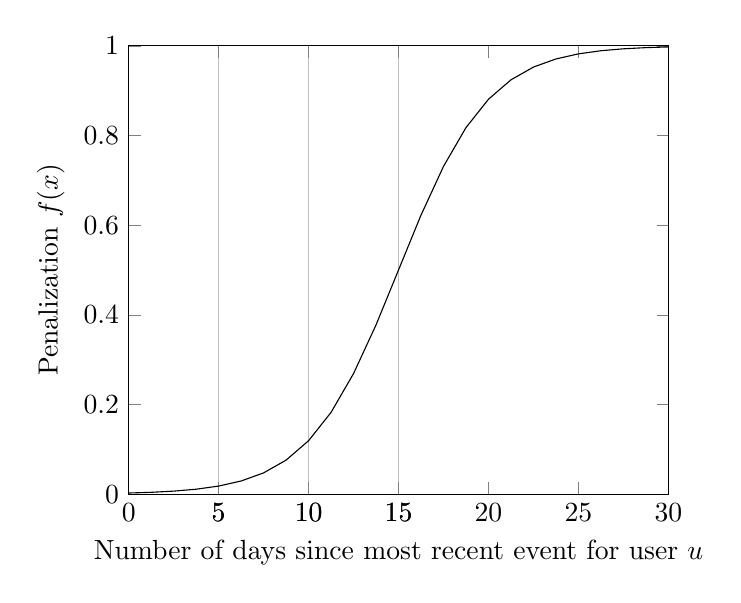
\begin{tikzpicture}
    \begin{axis}[
      ymin=0,ymax=1,
      xmin=0,xmax=30,
      xlabel=Number of days since most recent event for user $u$,
      ylabel=Penalization $f(x)$,
      extra x ticks={5,10,15},
      extra tick style={grid=major}
    ]
    \addplot[
    black,
    xlabel=$x$,
    ylabel=$f(x)$,
    domain=0:30]
    {1/(1+exp(-0.4*(x-15)))};
    \end{axis}
  \end{tikzpicture}
\end{figure}

As one can see, an event happening 15 days after the most recent event for user
$u$ will get a penalization of $0.5$ whilst an event with $x=5$ recieves
$0.018$. Following up on Table~\ref{events-example} we can calculate the
various penalizations and final scores for each day, by taking the highest
possible score for event $i$ and penalizing it in the following manner:

\begin{equation}
  s_{e}(x,u) = b_e - (b_e - w_e) \cdot p_{x}(u)
\end{equation}

where $p_x$ is the penalization after $x$ days. $b_e$ and $w_e$ are the best
and worst scores achievable for event $e$, respectivly. The final score
$s_{e}(x,u)$ is presented for each event below:

\begin{table}[H]
  \centering
  \begin{tabular}{llm{2cm}ll}
    \toprule
    Num. days ($x$) & Event types & Penalization $p_{x}(u)$ & Scores & Highest score \\
    \midrule
    5   & 1,2,3 & 0.018   & 59.1, 79.64, 99.64 & \textbf{99.64} \\
    10  & 1     & 0.1192  & 55.23              & 55.23  \\
    15  & 1,2   & 0.5     & 50.0, 70.0         & 70.0 \\
    \bottomrule
  \end{tabular}
  \caption[]{}
  \label{events-example}
\end{table}
\marginpar{Perhaps represent this differently?}

When selecting a score for user $u$ we select the highest valued one, in this
case 99.64. In fact, we can optimize our algorithm by starting at the most
recent events and not calculating scores for events types that yield a lower
score than the current highest score. In the scenario above we could take all
events on $x=5$, then taken the event type with highest maximum value (3) and
ignored all other events. Note that this is only true if you have
non-overlapping event type scores/intervals, as we have per
Table~\ref{implicit-example-scores}. We can now normalize $s$ and get a rating
$r$ between $a$ and $b$ by using the following equation, knowing that $X_{max}
= 100$ and $X_{min} = 0$:

\begin{equation}
  X' = a + \frac{(X-X_{min})\cdot(b-a)}{X_{max}-X_{min}}
  \label{eq-normalization}
\end{equation}

Setting $a$ to 0 and $b$ to 5, as is common in recommender systems we get the
rating $X' = 4.982$ when $s = 99.64$. Intuitivly this makes sense, if we assume
event type 3 to be the highest valued event in our system it would be
equivalaent to a user buying a product - or similar. Thus, if user $u$ bought
product $i$ only $5$ days ago this would get $4.98$ as final rating. If the
user does not interact with the product again in 30 days we can re-calculate
the score, now using $x=35$ which yields a penalization of $0.999$ and score $s
= 100-((100-80)*0,999) = 80.2$, normalized in the same likert scale as above we
get a new normalized rating $4.01$ - thus still a high rating, but not as
relevant for the user as 30 days earlier.

\subsection{Considering ordering of events}

In the our previous method using the number of days since the most recent event
we encounter several weaknesses when a user is either very active or have
events with a high degree of sparsity. In the latter a user interacting with
products every 20th day would see a divide in ratings since old events are
placed after at the top of the S-curve ($f(x) > 0.9$) and new events achieves a
penalization in the lower values ($f(x) < 0.1$). Similarily, when the user is
highly active we obtain a large number of items having the same penalization
weights and in essence a large duplication of ratings, provided the spread of
event types are not large, which in many systems are unlikely. One possibility
would be to use a finer granularity on the x values, such as seconds or minutes
since the most recent event, but instead we extend our method by not taking
into consideration the \textit{time}, but instead the \textit{ordering} of
events.

As before we use an example event log where we have 10 events of three
different types (1,2 and 3) on 6 different item IDs (1001-1006).

\begin{table}
  \centering
  \label{event-log-sigmoid-count}
  \begin{tabular}{lll}
    \toprule
    Ordering & Event type & Item id \\
    \midrule
    0 & 1 & 1001 \\
    1 & 1 & 1003 \\
    2 & 3 & 1002 \\
    3 & 1 & 1004 \\
    4 & 2 & 1002 \\
    5 & 2 & 1006 \\
    6 & 1 & 1005 \\
    7 & 1 & 1001 \\
    8 & 3 & 1005 \\
    9 & 1 & 1003 \\
    \bottomrule
  \end{tabular}
\end{table}

We want to continue using the sigmoid function, but in this case we will
differentiate based on how many events we observe for a user. Further, if a
user has e.g. more than 100 events in the event log we have two options: we can
set a ceiling, saying that events older than a threshold recieves the maximum
penalty or we can distribute all items evenly and extend the max-value of
x-axis. Probably one would want a combination of the two, having a pretty large
threshold and evenly distribute the items. In the case of evenly distribute the
values you would need a \textit{distribution factor} $f$ expressing the
relationship between steepness and shift coefficients. We use the following
equation where $c$ is the number of events for user $u$.

\begin{equation}
  f_{u}(x, c) =
    \begin{cases}
      1               & \text{if } c > 1000 \\
      \frac{1}{1+e^{-(f/c) \cdot (x - c)}} & \text{else }
    \end{cases}
\end{equation}

\subsection{Linearly blending the results}

\marginpar{Move this introduction to the pre-study?}
At this point we have found multiple novel ways of calculating the
implicit ratings, based on our implicit feedback. However, as one may observe
each method has its weknesses and strengths. A sigmoid-function considering the
number of days between events is good for including our implicit knowledge
about seasons into the ratings, but is not as effective if users has high
spread in between events or low activity. Further, there may exist some clothes
that has longer life-span than others, e.g. warm jackets that generally are
bought from September to March (7 months) compared to shorts which are
generally bought from May to August (4 months), depending on where the store
reside. Our second sigmoid function has the strength of always keeping the
ratings for a user fresh, also for less active users, but it is weaker in
differentiating between seasons - which can be seen if a user is on a hiatus
between January and August, not using the application. Upon return all ratings
would be based on his/hers winter activity, not penalizing the fact that the
type of clothes generally bought in the store at this time are different than
in January.

Optimally we would like to combine these two methods, taking their strenghts
and weaknesses together trying to average them out in order to end up with
generally better ratings - where we cannot trivally imagine scenarios as
depicted above where our models would fail. The process of combining such
ratings are in the Recommender Systems community called \textbf{blending} and
is in many ways a seperate research area in itself, if done advanced enough.
However, in the case of the naive and linear blend on can achieve results a
magninute higher than for each method seperatly as seen in \ref{}
\marginpar{find some refs using linear blending}.

When linearly blending $M$ models $m$, we choose $M$ factors $f$ all adding up
to 1.0, representing the weight of model $m_{i}$ in the final blend. Then when
calculating the final rating for item $j$ we sum over all models:

\begin{equation}
  r_j = \sum _{i=1}^{M} f_{i} * m_{j}
\end{equation}

As one may observe given the linear blend between with factors $f_1 = 0.7$ and
$f_2 = 0.3$ and the two ratings $m_1 = 5$ and $m_2 = 3$ for a given item, we
can calculate the final rating as $0.7 \cdot 5 + 0.3 \cdot 3 = 4.4$. A weakness
when linearly blending models in this way is the need for manually finding good
weights for the $M$ factors. There exists methods where this given a good test
set can be done automatically, such as using Linear Regression or KNN blending.
Many other blending schemes exists as well, such as Binned Linear Regression,
Bagged Gradient Boosted Decision Tree (BGBDT), Neural Networks and Kernel Ridge
Regression Blending \cite{jahrer2010combining} \cite{toscher2009bigchaos}.

As we have multiple proposed models we present our results given various
evaluation metrics and combinations of weights. Note that when a model has the
weight 1.0 its equal to that the model has not been blended with any other
model, and is included in the table below as a baseline.

\begin{table}[H]
  \centering
  \begin{tabular}{lll|ll}
    \toprule
    \textbf{Naive} &  \textbf{Sigmoid Count} & \textbf{Sigmoid Recent} &
    \textbf{RMSE} & \textbf{MAE} \\
    \midrule
    1.0  &      0.0        &      0.0       &  X   &  X  \\
    0.0  &      1.0        &      0.0       &  X   &  X  \\
    0.0  &      0.0        &      1.0       &  X   &  X  \\
    \midrule
    0.6  &      0.2        &      0.2       &  X   &  X  \\
    0.5  &      0.3        &      0.2       &  X   &  X  \\
    0.4  &      0.3        &      0.3       &  X   &  X  \\
    0.3  &      0.3        &      0.4       &  X   &  X  \\
    0.2  &      0.4        &      0.4       &  X   &  X  \\
    0.1  &      0.4        &      0.5       &  X   &  X  \\
    0.0  &      0.5        &      0.5       &  X   &  X  \\
    \bottomrule
  \end{tabular}
\end{table}

As one may see, the best results are achivied when blending with...
\marginpar{todo: analyze and finish this table}

% !TEX root = ../../report.tex
\clearpage
\section{Experimental Plan}

%We can sometimes evaluate how well the recommender achieves its overall goals.
%For example, we can check an e-commerce website revenue with and without the
%recommender system and thereby estimate the value of the system to the website.

This section will cover our experimental plan, starting off by looking at the
goals for our experiments. And how we want to get there. The remaining parts of
the section will describe the datasets used for evaluation, our evaluation methodology.
We have the following main goals for our experiment:

\begin{itemize}
	\item Determine the effect of utilizing multiple event types
	\item Determine whether our proposed implicit rating methods improve the recommendation quality over
	binary preference data.
	\item Evaluate the different implicit rating features and attempt to quantify their importance.
	\item Quantify the value of adding a cold-start solution method to the system.
	\item Propose a \emph{best} best combination of methods, given our current limitations for the SoBazar recommender system.
\end{itemize}

As baselines for our project we wish to first test a set of binary methods on the sobazar data
looking only at \emph{purchases}. We do the same for a binary dataset including the events
\emph{purchase}, \emph{wants} and \emph{likes}. We then want to test our \emph{implicit ratings}
considering different factors such as \emph{implicit factor weighting}, \emph{global popularity},
\emph{recency} and factors blended together using different schemes and see if they improve the
recommendation quality.

\subsection{Challenges}

%Every researchers wet dream - online system
The main problem with our experiment is the evaluation part. Namely, how can be determine
whether one set of ratings is better than another, and thereby validating our experiments?
The main reasons for implementing a recommender system is the desire to improve user
satisfaction and to increase the economic
success of a platform. Although both goals are interrelated they may be competing in some
scenarios. The user might be more interested in purchasing the products with the best
price-performance ratio, while the \emph{owners}
are more interested in showing the products that lead to the highest revenue for the
business. For this purpose, a commercial recommender could/should consider implementing
a reward attribute for items that show how much the company profits from its sale. However,
this is something that could be factored in during online testing at a later point.
The following figure shows an overview of the rating evaluation pipeline:

\begin{figure}[H]
		\centering
	  	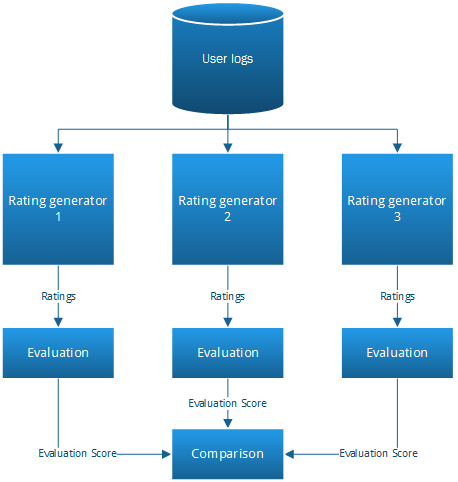
\includegraphics[height=0.65\linewidth]{image/ratinggeneval.png}
		\caption[Comparing Ratings]{The Figure shows the process of comparing ratings}
		\label{figure:compareratings}
\end{figure}

In order to further specify our goals we therefore have to take a closer look at the recommender's task,
its interface and the available data. The most typical task for a e-commerce recommender system is to
determine an order of items, often with the purpose of creating a top-k list of items that is shown in a sidebar
or on a dedicated page. The following figure shows the Sobazar newsfeed. Recommendations are likely
to be shown in a similar fashion. The interface currently initially shows four items, but lets the
user scroll sideways over up to 20 items.

\begin{figure}[H]
		\centering
		\begin{minipage}{.45\linewidth}
	  		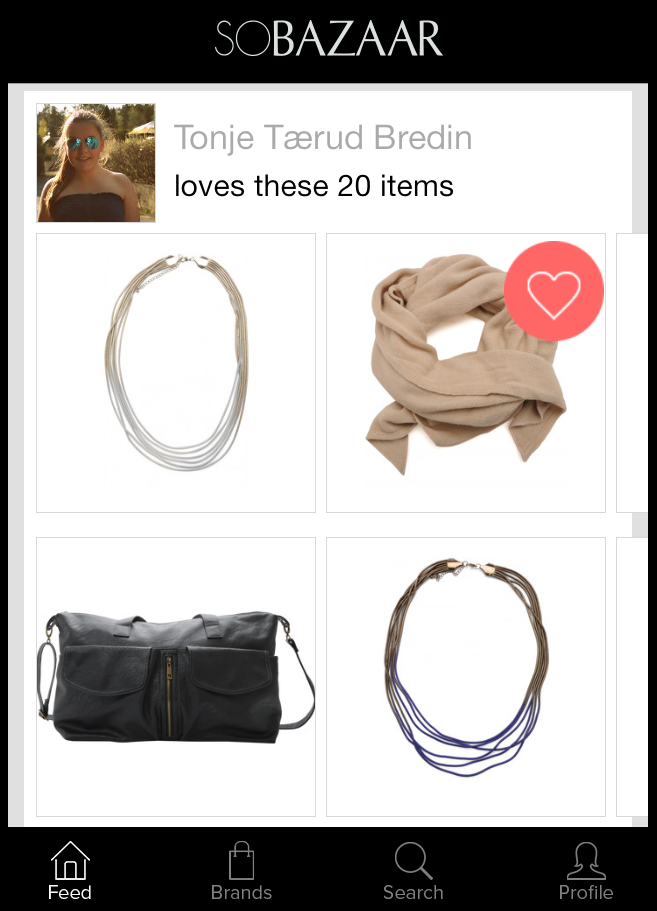
\includegraphics[height=1.2\linewidth]{image/SoBazaarfeed2.png}
		\end{minipage}
		\begin{minipage}{.45\linewidth}
			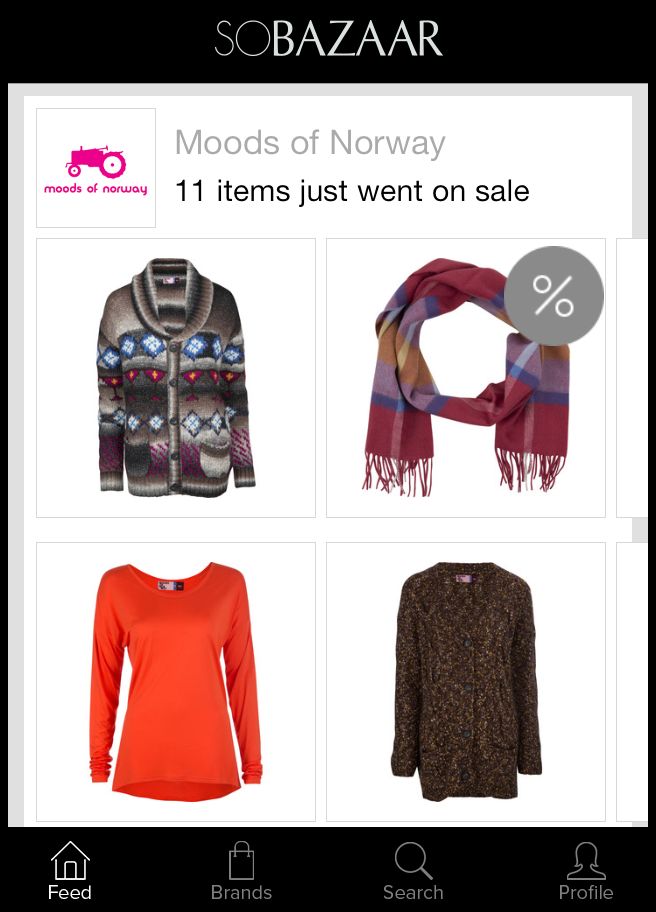
\includegraphics[height=1.2\linewidth]{image/SoBazaarsale.png} 
		\end{minipage}
		\caption[Sobazaar News Feed - Version 0.5.1]{SobBazaar news feed items}
		\label{figure:sobazarfeed}
\end{figure}

Ultimately, the goal of the experiment is to evaluate and measure the properties
of the system, which we have identified as the most important for the systems success,
and select the method that performs the best overall with respect to these properties.

\subsubsection{Dataset}

In addition to evaluate the methods on the Sobazar dataset we want to make sure that our
methods generalizes beyond our experimental dataset, in accordance to the general guidelines
for experimental studies \cite{Shani2011}. The data used for offline evaluation should match
as closely as possible the data we expect the recommender system to face when it is
deployed \cite{Gunawardana2009}. When selecting datasets for evaluation we focused on the
following dataset properties:

\begin{itemize}
	\item Size of dataset: Preferable as close as possible to Sobazar or larger (a few months from now)
	in terms of number of ratings, users and items.
	\item Different different types of implicit factors	such as clicks, likes and purchases.
	\item Domain: Preferably a domain as close to possible as the e-commerce domain where
	factors like recency also would apply.
	\item Timestamps: To evaluate the recentness mapping
	\item Presence of features (Secondary)
\end{itemize}

We were unable to acquire any e-commerce datasets containing user browsing history, purchases etc.
Thus making the main contributions of this article untestable, thus rendering further experiments
on other datasets useless. It is worth nothing that we inquired other researchers having
experimented with similar datasets to no luck.

\paragraph{The Sobazar Dataset}

The Sobazar dataset is small and sparse dataset. When looking only at the purchases
we have a total of 1,592 binary ratings given by 466 users to 1188 items. When including
clicks, wants and purchases we end up with 27,873 ratings given by 1,511 users to 5,855 items.
We also have access to semi-structured product information collected/crawled from
the online retailers for \emph{a majority} items.

Having such a small and sparse dataset has several implications. Firstly we have
to avoid \emph{wishful thinking} as we have very thin data, meaning that we cannot
rely on getting reliable results. Secondly, our evaluation methodology must be
\emph{tailored} for small sparse datasets. E.g. when using cross-validation the number
of folds depends on the size of the dataset. For large datasets, even 3-fold Cross
validation will be quite accurate, while for very sparse datasets, one may have to
use leave-one-out in order to train on as many examples as possible. The advantages
of using a large number of folds is that the bias of the true error rate estimators
will be small, meaning that the estimator will be very accurate, with the disadvantages being that
the variance of the true error rate estimator will be large in addition to increased
computation time. Another alternative well suited for sparse datasets is the \emph{all but one} or the
\emph{leave one out} method, in which we remove one rating from the test users
and try to predict the hidden rating.

Another important concern is whether or not to take the timestamps into consideration,
which directly speaks against the use of cross-validation, as we wish to use the past
interactions to predict future actions. When using the \emph{leave one out} method one
could e.g. always remove the users freshest rating and try to predict it and repeat the
process any number of times. This is particularly relevant as some of our implicit mapping functions
factors in recency.

\subparagraph{Overview of the Dataset}

Table \ref{table:datasets} shows an overview of the sobazar dataset.

%TODO - What else is interesting to know? Rating scale, average number of ratings per user, number of cold start users...
%TODO - % of users with less than 5 ratings for both datasets

\begin{table}[H]
    \centering
    \begin{tabular}{l l l l l l }
    \toprule
	Dataset						& 	Ratings		& 	Users		& 	Items 		& 	Sparsity			& Rating Scale 				    \\ \midrule
	Sobazar	(Purchases Only) 	&	1,592		&	466			&	1188		&	99.71243			& Binary						\\
	Sobazar (All events)		& 	27,873  	& 	1,511		&	5855		& 	99.69657			& Binary/Implicit Ratings		\\ 
	%Movielens 1M				& 	1,000,029   &	6040 		&	3706		&	95.53164			& Explicit (1-5)				\\ 
	\bottomrule
    \end{tabular}
    \caption [Overview of the datasets used for evaluation]{Overview of the datasets used for evaluation}
    \label{table:datasets}
\end{table}

As you can see the recommender can cover a much larger portion of the user group and items when including multiple event types.

\subsection{Comparing Ratings}

The success on our experiment mainly relies on whether we can successfully compare a set of ratings.
Evaluating and comparing a set of ratings is not something you often encounter in the literature. And the
bottom line is that evaluating and comparing a set of ratings is hard. However, we have a few theories on
how it can be done:

\begin{enumerate}
\item Can we put the ratings into a traditional recommender system evaluation pipeline and use the
	  results from that to compare the ratings. In that case, what evaluation metrics are suitable?
\item User studies. Ask users to evaluate how well the produced ratings fit their actual preferences \cite{parra2011walk}.
\item Online experiments measuring e.g. the increased revenue generated or the click-through-rate.
\end{enumerate}

Where we \emph{chose} to go for the first alternative, despite its obvious weaknesses. User studies
are expensive and we simply do not have the time or resources to interview hundreds of actual users.
We do also not have the option of performing any online experiments. Either way it would be best to
get some kind of validation on our results before deploying the system to minimize the risk of giving
low-quality recommendations to the users.

We could say that we believe that better ratings gives us better recommendation results, and use this
as a basis for our evaluation. However, this means that the results we get from testing them
on different algorithms should be comparable. There are two main problems with this. The first is that
we rely on a recommender algorithm can make use of our implicit ratings. We also need to be careful
when selecting evaluation metrics. Many evaluation metrics consider supplied ratings as the \emph{ground truth}
and bases its evaluation score on these numbers. This automatically disqualifies any evaluation metrics
that consider the rating values such as e.g. MAE. After some thought and consideration
we identified the following properties as the best indicators of improved recommendation quality.

\begin{itemize}
\item Does it improve the recall?
\item Does it improve the recommenders ability to rank the items?
\end{itemize}

A further discussion on evaluation metrics will follow in the next Section \ref{sec:eval-metrics}.

\subsubsection{Purchase Only Vs. Multiple Implicit Factors}

\marginpar{I cannot see how we possibly can compare these two...}

We want to evaluate whether a recommender system utilizing multiple implicit factors outperform
a recommender system utilizing purchase data only.
How, then, do we determine one as better than the other? We can see the following challanges:
Firstly, we have two different datasets, as one contains 1045 users and 4667 items more than the
other. How much should the additional coverage factor in? How do we treat the items and users
occurring only in one dataset when evaluating? How do we \emph{treat} the events types only
occurring in one dataset? Only \emph{sensible} thing to do is to compare the purchased items
in some way, the question is how? Currently we can not see how we possibly could compare the
two using traditional offline evaluation methods. Meaning that our comparison of the two will
be made on somewhat of a \emph{subjective} basis.
	
\subsubsection{Comparing Binary and Non-Binary Models}

\marginpar{The question then, is how critical this flaw is to our experiment}
We want to quantify the improvements if any from using implicit ratings over binary ratings.
The main challenges of comparing the binary ratings with the non-binary ones are the fact
that the models for making recommendations differ. Optimally you would like to fix every
\emph{variable} when doing this comparison, however, it is not possible in this case.
To \emph{solve} this problem we decided that the best solution was to select \emph{state-of-the-art}
methods from both classes and compare their results. Worst case scenario we find out that the
methods for non-binary implicit feedback are not as \emph{good} as the binary models and thus
should not be used.

\subsubsection{Comparing Implicit Rating Methods}

%What we want to do
We want to figure out how to evaluate and compare the different implicit rating methods. 
The most obvious solution here would be to analyze the amount of purchases, wants and clicks
in the recommendation lists individually. This is mainly a evaluation metric problem. Which
will be discussed at length in the next Section.

%Challanges/Problems of actually doing it
%How can we determine if one set of recommendations is better than another?
%	- Evaluation metric problem
%	- One obvious solution would be to analyze the amount of purchases, wants and clicks
%	  in the recommendation lists individually.
%	  	- How much at the list do we take into consideration?
%	  		- 20 is a pretty obvious choice based on the UI of the application
%	  	- How do we weight the different events
%	  	- How do we determine the positional importance of the recommendations?
%	  		- Always recommending purchases in the top positions is better than
%	  		  recommending clicks, but how much better exactly?
%How do we plan to solve them
	%Assumptions & Weaknesses


\subsection{Combining Implicit Ratings With Existing Cold-Start Solutions}

%Only use cold-start splits for this sections tables.

After the best method have been chosen we wish to further improve our results by adding
a cold-start solution to our system. In the second stage of our experiment we wish
to see if we can apply a cold-start solution to increase the systems cold-start performance.
Here we also wish to factor in factors such as recency to see whether or not connecting
new users with the most popular items for the $k$ last weeks, instead of the entire
period further can improve the cold-start performance of the system. Similarly
for our criticBot where we can select the most active users for the $n$ last weeks.

\subsubsection{Simulating the Cold-Start Problem}

To simulate the cold-start problem and evaluate how well our the different
methods tackle the different cold-start situations we use the following
evaluation methodology. As mentioned in Section \ref{sec:cold-start-eval} there is
no common framework for assessing the cold-start performance of recommender systems.
Our goal is to come up with \emph{comprehensive} framework to assess the cold-start
performance of our recommender systems. The following inputs changes the dataset over time:

\begin{itemize}
	\item 	Existing users watch new items in the catalogue
	\item	New users join the system and view their first item
	\item	New items are added to the catalogue
\end{itemize}

The first input source has the effect of increasing the dataset density, the average user
profile length, and the average number of views per item. The second input factor has
the effect of decreasing both the dataset density and the average user profile length,
as the new users that join the system have interacted with only a few items. Similarly,
the third input factor has the effect of decreasing both the dataset density and the average
number of views per item.

To simulate the cold-start user problem we propose splitting the users into two disjoint
sets, similarly as in \cite{Stern2009, Lam2008}, using 90\% of the users for training and
setting aside the remaining 10\% for evaluation. We then train the model with e.g. 5, 15,
25 and 35 of the test users ratings and give predictions for all models. Alternatively one could train the model
using e.g. 25\% and 75\% of each test users ratings. Similarly, to simulate the cold-start
item problem we again split the items into two disjoint sets, using 90\% of the items
for training and the remaining 10\% for evaluation.  We then train the model with
e.g. 20, 40, 60 and 80 ratings and predict the remaining values. The selection criteria
for test items and users can differ from dataset to dataset. E.g. in \cite{Rashid2002, Rashid2008}
the authors selected a subset of the users with more than 200 ratings, but you can not
expect 10\% all the users for all datasets to have provided 200 ratings, so this number
might be lowered if necessary. The implications of removing the top 10\% of the
raters from the Sobazar dataset is fairly large as they stand for a large portion
of the few ratings we have.

To evaluate the cold-start system performance we use the same method as described
in ~\cite{Agarwal2009} where the authors propose using a 75:25 training/test split,
where we at random draw e.g. 35\%, 50\% and then finally use all (75\%) of the
ratings in the training set and predict the remaining 25\%.

%How is this implemented on the sobazar data?

For the Sobazar dataset we select 10\% of the users as test users, for a user to be
selected as a test user, the user must have provided at least 20 ratings. The test user are drawn
at random from the eligible candidates. We then train
the model using 10\%, 40\% and 75\% of their ratings and try to predict their remaining ratings.
The reason for choosing percentages over hard limits is due to the fact that the ratings are
distributed unevenly among the users. As we have a very low number of ratings and a large item collection we had to use
only 5\% of the items as test items, where each test item have been rated by atleast 15 users.
We train the model using 10\%, 40\% and 75\% of their ratings and try to predict their remaining
ratings. As we have access time timestamps, we split the users and items based on timestamp.
E.g. for the 10\% user split we train the model with their initial ratings and try to predict
their following ratings. To evaluate the cold-start system performance we split the dataset in a test
and training set using 20\% of the ratings for testing and then train the model
using 40\%, 60\% and 80\% of the ratings for training. It is important to note that
this process should be repeated multiple times, as the chance of getting an
\emph{unfortunate} split is highly probable due to the dataset size. For the cold-start
system task we also split the dataset based on timestamps, meaning that the test set consists
of the most recent ratings.





\begin{center}
    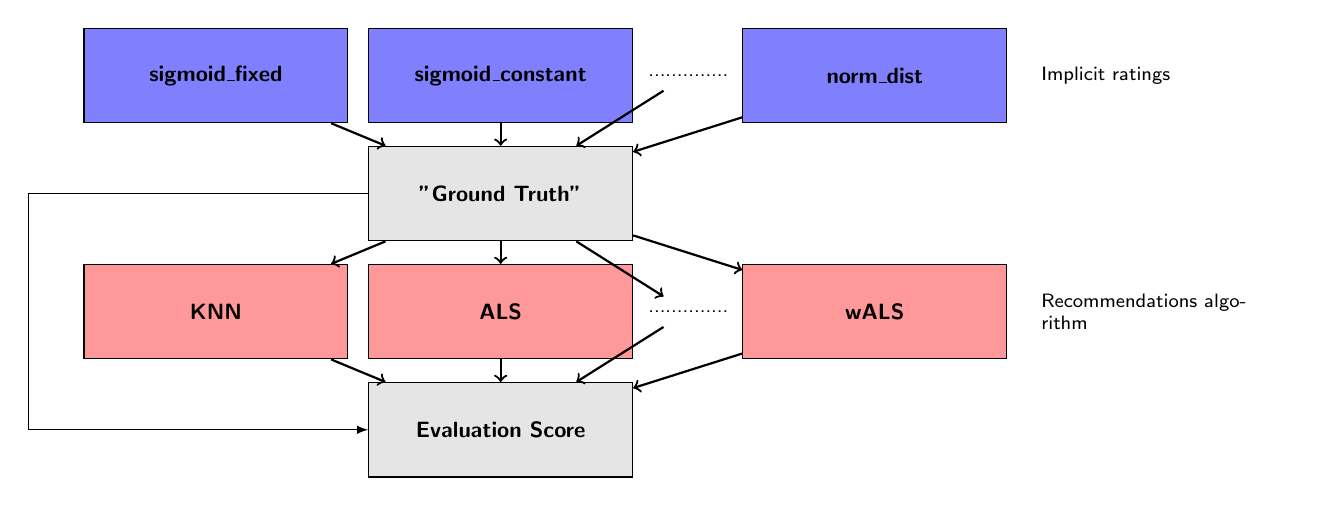
\begin{tikzpicture}
		[node distance = 1cm, auto,font=\footnotesize,
		% STYLES
		every node/.style={node distance=1.5cm},
		% The comment style is used to describe the characteristics of each process
		comment/.style={rectangle, inner sep= 5pt, text width=3cm, node distance=0.25cm, font=\scriptsize\sffamily},
		% small comment lol
		comment-small/.style={rectangle, inner sep= 5pt, text width=1cm, node distance=0.25cm, font=\scriptsize\sffamily},
		% The nonProcess style
		nonProcess/.style={rectangle, draw, inner sep=5pt, text width=3cm, text badly centered, minimum height=1.2cm, font=\footnotesize\sffamily},
		% The process style is used to draw the processs' name
		process/.style={rectangle, draw, fill=black!10, inner sep=5pt, text width=3cm, text badly centered, minimum height=1.2cm, font=\bfseries\footnotesize\sffamily},
		% ratingsGenerator style
		ratingsGenerators/.style={rectangle, draw, fill=blue!50, inner sep=5pt, text width=3cm, text badly centered, minimum height=1.2cm, font=\bfseries\footnotesize\sffamily},
		% racommendation algorithms
		recAlgs/.style={rectangle, draw, fill=red!40, inner sep=5pt, text width=3cm, text badly centered, minimum height=1.2cm, font=\bfseries\footnotesize\sffamily}]

		% Draw processs
		\node [ratingsGenerators] (rg1) {sigmoid\_fixed};
		\node [ratingsGenerators, right=0.25 of rg1] (rg2) {sigmoid\_constant};
		\node [comment-small, right=0.01 of rg2] (dotdotdot) {..............};
		\node [ratingsGenerators, right=0.01 of dotdotdot] (rg3) {norm\_dist};

		\node [process, below of=rg2] (gt) {"Ground Truth"};

		\node [recAlgs, below of=gt] (ra2) {ALS};
		\node [recAlgs, left=0.25 of ra2] (ra1) {KNN};
		\node [comment-small, right=0.01 of ra2] (dotdotdot2) {..............};
		\node [recAlgs, right=0.01 of dotdotdot2] (ra3) {wALS};

		\node [process, below of=ra2] (eval) {Evaluation Score};

		% \node [nonProcess, below of=implicitConverter] (ratings) {Ratings for the items};
		% \node [process, below of=ratings] (recommendations) {Make recommendations};
		% \node [process, below of=recommendations] (evaluations) {Evaluate recommendations};
		% \node [nonProcess, below of=evaluations] (evaluationValue) {Recommendation score};

		%%%%%%%%%%%%%%%
		% Comments
		\node [comment, right=0.25 of rg3] (comment-rg3) {
			Implicit ratings
		};
		\node [comment, right=0.25 of ra3] (comment-ra3) {
			Recommendations algorithm
		};
		% \node [comment, right=0.25 of ratings] (comment-ratings) {
		% The output of the conversion is a set of ratings on the different items from the soBazar dataset
		% };
		% \node [comment, right=0.25 of recommendations] (comment-recommendations) {
		% Makes recommendations based on the inputed ratings. Different approaches to make the recommendations can be take, such as matrix factorization or neighborhood based approaches
		% };
		% \node [comment, right=0.25 of evaluations] (comment-evaluations) {
		% Evaluate the recommender system(s). Different evaluation metrics will be usea, such as e.g. AUC and nDCG
		% };

		%%%%%%%%%%%%%%%%
		% Draw the links between processs
		\path[->,thick]
			(rg1) edge (gt)
			(rg2) edge (gt)
			(dotdotdot) edge (gt)
			(rg3) edge (gt)
			(gt) edge (ra1)
			(gt) edge (ra2)
			(gt) edge (dotdotdot2)
			(gt) edge (ra3)
			(ra1) edge (eval)
			(ra2) edge (eval)
			(dotdotdot2) edge (eval)
			(ra3) edge (eval);
		% \path[>=latex,->] (gt) edge (eval);
		% \draw[rectangle connector=-3cm] (gt) to (eval);
		\draw[>=latex,->] (gt) -- +(-6,0) |- (eval);
    \end{tikzpicture}
    \captionof{figure}[Implicit Rating Evaluation]{Overview of how the generated ratings from the implicit feedback can be evaluated.}
  	\label{figure:implicitRatingEvaluation}
  \end{center}

The blue boxes in figure~\ref{figure:implicitRatingEvaluation} are functions used to produce the implicit ratings based on the implicit feedback. Based on this, the system gets an estimated \emph{ground truth}, which can be used to evaluate the different recommendation algorithms show in the red boxes. Based on the evaluation score something can be said about the implicit feedback conversion to implicit ratings and the recommendation algorithms used.









\section{Evaluation Metrics}
\label{sec:eval-metrics}

%http://www.slideshare.net/gunnar-schroeder

A large variety of metrics have been published, and some of these metrics are highly correlated \cite{Herlocker2004}.
There is little guidance for evaluating recommender systems and choosing metrics. However, there are
some important questions one should ask oneself when selecting evaluation metrics:

\begin{itemize}
	\item Which aspects of the usage scenario and the data influence the choice?
	\item Which metrics are applicable?
	\item What does these metrics express?
	\item What are the differences among them?
	\item Which metric represent our user-case best?
	\item How much do the metrics suffer biases?
\end{itemize}

It is safe to assume that the users are more interested in the top ranked items, than rating
predictions for the entire item collection. The social feed shown in Figure \ref{figure:sobazarfeed}
shows that the interface currently supports showing up to 20 items.

\begin{figure}[H]
  \centering
  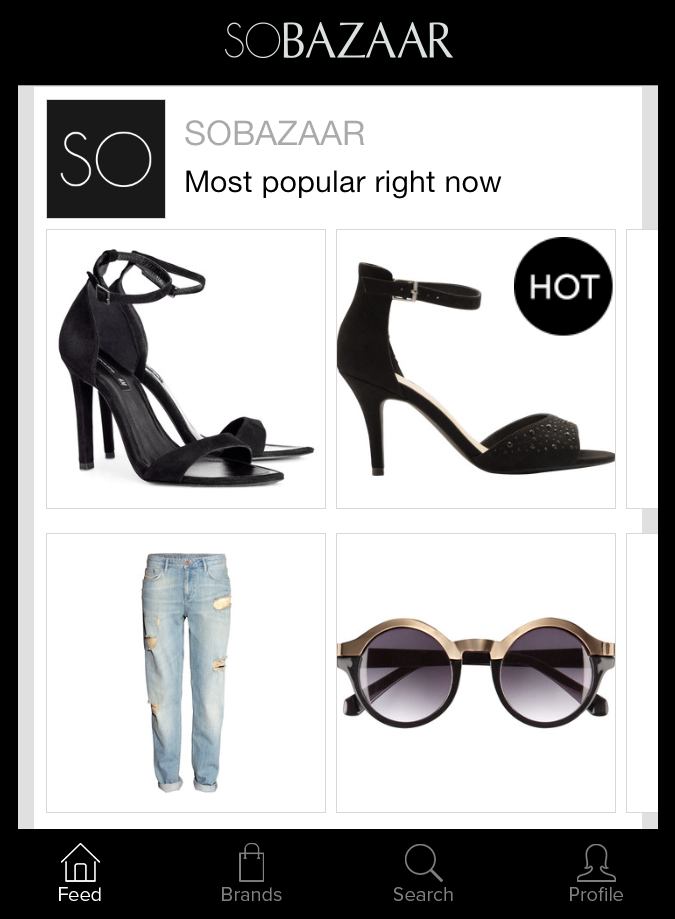
\includegraphics[height=.5\linewidth]{image/SoBazaarmostpop.png}
  \caption[Sobazar most-popular recommendation]{The Figure shows how the most-popular recommendations are shown in the application}
\label{figure:mostpopular}
\end{figure}

Evaluation of top-k recommendations suggests a classification or ranking task, the evaluation
should therefore focus on classification or ranking accuracy. A classification accuracy metric
will tell us something about the recommenders ability to retrieve relevant items. The ranking
accuracy metric should measure how well the different methods are at putting the most relevant items
e.g. purchases consistently over the assumed less relevant ones such as e.g. clicks. This gives us
two hints with regards to our evaluation: (1) a ranking accuracy that measures the overall ranking
is not appropriate, (2) the ranking accuracy metric should be able to factor in difference relevance
values for the different event types.

%TODO - Add some more cites

\subsection{Accuracy Metrics}

The Area Under Curve (AUC) is a popular classification accuracy metric. ROC curves provide a graphical
representation for the performance of a recommender system, by plotting the recall (true positive rate)
against the fallout (false positive rate) for increasing recommendation set size. A perfect recommender
would therefore yield a ROC curve that goes straight up towards 1.0 recall and 0.0 fallout until all
relevant items are retrieved. Afterwards it would go straight towards 1.0 fallout while the remaining
irrelevant items follow. One therefore obviously aims to maximize the area under the curve (AUC). The higher
up all relevant items (true positives) are in the recommendation list, the higher the AUC score.
AUC can therefore be used as a single measure for the overall quality of a recommender system. Table \ref{table:auc}
shows an example of the AUC values when varying the position of a single relevant document through the
recommendation list.

\begin{table}[H]
	\centering
	\begin{tabular}{*{12}l}
	\toprule
	\#Example	& R1 & R2 & R3 & R4 & R5 & R6 & R7 & R8 & R9 & R10 & AUC \\ \midrule
	1		& \cmark & \xmark & \xmark & \xmark & \xmark & \xmark & \xmark & \xmark & \xmark & \xmark & 1.000 \\ 
	2		& \xmark & \cmark & \xmark & \xmark & \xmark & \xmark & \xmark & \xmark & \xmark & \xmark & 0.889 \\ 
	3		& \xmark & \xmark & \cmark & \xmark & \xmark & \xmark & \xmark & \xmark & \xmark & \xmark & 0.778 \\ 
	4		& \xmark & \xmark & \xmark & \cmark & \xmark & \xmark & \xmark & \xmark & \xmark & \xmark & 0.667 \\ 
	5		& \xmark & \xmark & \xmark & \xmark & \cmark & \xmark & \xmark & \xmark & \xmark & \xmark & 0.556 \\ 
	6		& \xmark & \xmark & \xmark & \xmark & \xmark & \cmark & \xmark & \xmark & \xmark & \xmark & 0.444 \\ 
	7		& \xmark & \xmark & \xmark & \xmark & \xmark & \xmark & \cmark & \xmark & \xmark & \xmark & 0.333 \\ 
	8		& \xmark & \xmark & \xmark & \xmark & \xmark & \xmark & \xmark & \cmark & \xmark & \xmark & 0.222 \\ 
	9		& \xmark & \xmark & \xmark & \xmark & \xmark & \xmark & \xmark & \xmark & \cmark & \xmark & 0.111 \\ 
	10		& \xmark & \xmark & \xmark & \xmark & \xmark & \xmark & \xmark & \xmark & \xmark & \cmark & 0.000 \\
	\bottomrule
	\end{tabular}
	\caption{Varying the position of a single relevant item on a four out of ten recommendation list}
	\label{table:auc}
\end{table}

One should also be aware of that the AUC scores can be highly inaccurate, especially for cold-start users,
users which the recommender is unable to provide more than a handful of recommendations for. AUC requires
a total ordering of all items not yet rated by the user. This means that the items not recommendable
to the user will be appended in a random order after the known recommendations.
E.g. lets say the recommender is able to generate 10 recommendations for a user out of 4000 items.
The recommender was only able to retrieve one out of two relevant test items. The remaining 3990
items are therefor appended in random order to the users recommendation list.
Where the last test item is appended in the recommendation list can mean the difference between a AUC score of above
0.9 to less than 0.6 if the item is appended at the end of the list, the results can be even more
severe if none of the items is in the initial recommended list, then the results for that user will be
completely random. The most obvious solution to this problem would be to use resampling or to repeat
the experiment multiple times where the order of the items not in the recommendation list are drawn at random and
the results averaged over all the trials.

However, a frequently uttered point of criticism is that users are often more interested in the items
at the top of a recommendation list but that the AUC measure is equally affected by swaps at the top
or the bottom. To \emph{complement} AUC, we also wish to measure the rank accuracy to get a better
overall picture of the systems performance. This means that we want to measure whether or not
highly rated items such as purchases, likes etc. are ranked higher than less relevant items such as clicks,
as having these highly ranked items higher up in the recommendation list aligns with our previously
mentioned financial incentives.

%TODO - What is the "best" rank-accuracy metric?

\subsection{Rank accuracy}

\marginpar{TODO: Move to evaluation section?...}

When using rank accuracy metrics, it is worth knowing whether one is measuring total or partial orderings.
Most rank accuracy metrics (e.g. Kendall's tau and Spearman's rho) compare two total ordering. The problem
with these measures is that we in most cases are not provided with a full ranking of the items as most recommendation
algorithms only generate a partial list of items that are likely to be preferred by a user. The remaining items
would therefore have to be concatenated in random order. The recommendation list can also consist of several
items with similar rating that can appear in varying orders. Therefore, in order to create a full ranking of
the items all preference values for the user have to be known. Since the user can express the same rating for similar
items, the list will again contain groups of items that can appear in arbitrary order. However, the largest problem
is posed by items for which no rating is known. These items could hold an arbitrary place within the ranking.
Again, consider an example where a user e.g. have rated 5 items out of 4000, and the recommender is able to recommend
only 10 items for that user. To measure the rank accuracy we would have to randomly add 3995 items to the users known
preference list and 3990 to the users prediction list. Comparing the order of these lists would not make much sense.
The bottom line is that in most cases a rank metric for partial ordering would be more appropriate for comparing
recommendation lists that are produced by recommenders to item rankings from known user preferences.

We assume that we can recommend at most $k$ items for each user at a time. It also pays to submit all $k$
recommendations, because we are not penalized for bad guesses. We also assume that the order matters, so it
is better to submit more certain recommendations first, followed by recommendations we are less sure about.
Which means that we basically select the $k$ best candidates in order.
However, a problem is that the likeliness of finding a \emph{hidden} item in e.g. the top 20 recommended items
is not very large when one is working with large item catalogs. The problem then, is how to select the value of $k$.
Setting it to low you risk ending up with many $0.0$ values, and when setting it to high you risk including to many
\emph{randomly} concatenated ratings in the results. We believe a value of \textit{20} is natural choice for our
application as up to 20 recommendations can be shown in the user interface.

Mean average precision (MAP@k), described in Section \ref{subp:mean_average_precision_map_} is a popular metric for search
engines and is applied, for example, to report results at the Text Retrieval Conference (TREC). The main weakness with regard
to recommender systems is that it assumes that the user is interested in finding many relevant documents for each query, and
does not look at the relevance of the items. Consider the following examples where we have three lists of hidden items and
three recommendations lists. All none relevant items are labeled with the item-id $0$.

\begin{table}[H]
\label{table:ap}
\centering
\begin{tabular}{*{4}l}
\toprule
Example 	& 	Actual					& 	Recommended					&	AP@10   \\ \midrule
1			& [1,2,3,4,5,6,7,8,9,10]	&	[1,0,0,0,0,0,0,0,0,0]		&	0.100  \\ 
2			& [1,2,3,4,5,6,7,8,9,10]	&	[1,0,0,0,2,0,0,0,0,0]		&	0.140  \\ 
3			& [1,2,3,4,5,6,7,8,9,10]	&	[8,0,0,0,9,0,0,0,0,0]		&	0.140  \\
4			& [1,2,3,4,5,6,7,8,9,10]	&	[1,0,0,0,3,0,5,0,0,0]		&	0.183  \\ 
5			& [1,2,3,4,5,6,7,8,9,10]	&	[0,0,0,2,0,0,0,6,5,0]		&	0.083  \\ 
6			& [1,2,3,4,5,6,7,8,9,10]	&	[0,0,0,0,7,0,8,0,0,0]		&	0.049  \\
7			& [1,2,3,4,5,6,7,8,9,10]	&	[0,0,0,0,7,0,0,0,0,1]		&	0.040  \\ 
8			& [1,2,3,4,5,6,7,8,9,10]	&	[0,0,0,0,0,0,0,8,5,0]		&	0.035  \\ 
9			& [1,2,3,4,5,6,7,8,9,10]	&	[1,3,4,5,6,0,0,0,0,0]		&	0.500  \\
10			& [1,2,3,4,5,6,7,8,9,10]	&	[0,0,0,0,0,1,2,8,5,3]		&	0.178  \\ 
\bottomrule
\end{tabular}
\caption{AP@10 Examples}
\end{table}

As you see from example two and three average precision does not consider the order of the actual item list. We want some way to
reward the recommender for getting the purchased ranked higher than both wants and clicks.


Normalized Discounted Cumulative Gain (nDCG) described in Section \ref{subp:normalized_discounted_cumulative_gain_} is another metric to
measure the rank accuracy. It is based on two main assumptions; (1) Highly relevant items are more useful than marginally relevant ones,
(2) The lower the ranked position of a relevant item, the less useful it is for the user, since it is less likely to be \emph{examined}.
The maybe most interesting aspect of nDCG is that it contains an utility function $rel_i$. One can replace the original utility function
and replace it with a function that is more suited to the application. One could e.g. assign the relevance of an item using
the following functions:

\begin{itemize}
\item $rel_i = 1/log(i+k)$, where i is the index of the item in the actual sorted rating list, where $k$ is a constant.
\item $rel_i = u(i)$, simply assign a relevance or utility score.
\end{itemize}

The latter would have been perfect, given that we could specify the importance of each event e.g. purchase gets a relevance of 3, want
a relevance of 2 and a click a relevance of 1, as it would give us a single number on the ranking quality of the recommendations.
However, we do not not know these values, meaning that nDCG cannot be used without making assumptions of the importance of the different
event types.

\marginpar{Mention why we think it is wrong to make these assumptions?}

To solve this problem we decided to chose a \emph{simpler} approach. We separately measure the recall for purchases, wants and
clicks separately in addition to measuring the MAP\@20 scores for the different event types. Given that we have known the relevance of
the different event types nDCG could have given us all these numbers summarized in one column, instead we now have twelve. 

By combing the AUC which gives us the recall for the entire recommendation list for each user, the MAP\@20 to measure the precision of
the top 20 recommendations and then give individual numbers for the different event types we believe we would get a good overview of
the systems overall performance with the main emphasis on the top 20 recommendations.

%Normalized Discounted Cumulative Gain ($nDCG_{k}$), described in Section \ref{subp:normalized_discounted_cumulative_gain_}
% 
%
%For our application we believe it to be beneficial to use the rating of the item as a
%relevance score, as we could have multiple items with highly similar ratings (thus the same relevance). When using a low $k$ value for the logarithmic alternative this could mean that the relevance between two almost similarly rated items might end up being disproportionately large. We will also most likely look at the 20 top items, which means that the difference between the lower ranked items will be fairly small, as the logarithmic function converges. A third alternative would be to also use some linear decay function. The following table shows the $nDCG$ score for a set of examples where the function $rel_i = 1/log(i+1)$ is used to assign the relevance score to item $i$ in the sorted list of actual ratings. E.g. item one is assigned a relevance score of $1/(log(2)$ and so on. We hope the following table will give the reader a better idea of how $nDCG$ \emph{works}.
%
%\begin{table}[H]
%\label{table:ndcg}
%\centering
%\begin{tabular}{*{4}l}
%\toprule
%Example 	& 	Actual					& 	Recommended				&	nDCG 	\\ \midrule
%1			& 	[1,2,3,4]				&	[1,0,0,0]				&	0.470   \\ 
%2			& 	[1,2,3,4]				&	[2,0,0,0]				&	0.360   \\ 
%3			& 	[1,2,3,4]				&	[3,0,0,0]				&	0.330   \\ 
%4			& 	[1,2,3,4,5,6,7,8,9,10] 	& 	[1,2,3,4,5,6,7,8,9,10] 	&   1.000	\\ 
%5			& 	[1,2,3,4,5,6,7,8,9,10] 	& 	[10,9,8,7,6,5,4,3,2,1] 	&   0.900	\\ 
%6			&	[1,2,3,4,5,6,7,8,9,10] 	& 	[1,2,0,0,0,0,0,0,0,0] 	&   0.440	\\ 
%7			& 	[1,2,3,4,5,6,7,8,9,10] 	& 	[1,0,0,3,0,0,0,0,0,0] 	&   0.390	\\ 
%8			& 	[1,2,3,4,5,6,7,8,9,10] 	& 	[4,0,0,0,8,0,0,0,0,0] 	&   0.280	\\ 
%9			& 	[1,2,3,4,5,6,7,8,9,10] 	& 	[0,0,0,0,5,0,0,0,0,10] 	&   0.130	\\ 
%10			& 	[1,2,3,4,5,6,7,8,9,10] 	& 	[0,0,0,0,0,0,0,0,9,10]	&   0.110	\\
%\bottomrule
%\end{tabular}
%\caption{nDCG Test Examples}
%\end{table}
%
%As you can see from the above mentioned examples nDCG will give us an indication whether or not our recommender
%ranks \emph{highly relevant} items above those who are less relevant. As for the limitations, nDCG is designed for situations of non-binary notions of relevance, thus it cannot be used in our experiment where we wish to compare binary ratings with implicit ratings. The main difficulty encountered in using nDCG is the unavailability of an ideal ordering of results when only partial relevance feedback is available. This is often the case when we have several equally good results. This is especially true when the metric is limited to only first few results as it is often done in practice.
%
%We chose take a closer look at the different ways of calculating nDCG. There are two commonly used methods used to calculate the DCG and IDCG scores.
%
%\begin{itemize}
%\item Method 1  $DCG_p = rel_1 + \sum_{i=2}^{p} \frac{rel_i}{log_2(i)}$
%\item Method 2: $DCG_p = \sum_{i=1}^{p} \frac{2^{rel_i}-1}{log_2(i+1})$
%\end{itemize}
%
%The following table shows the differences between Method 1 and Method 2 on a few selected examples. Here we set the value of $rel_i$ equal to the implicit rating of item $i$.
%
%\begin{table}[H]
%\label{table:ndcgfinal}
%\centering
%\begin{tabular}{*{5}l}
%\toprule
%\#Ex & 	Actual																		& 	Recommended				&	$nDCG^1$  	   & $nDCG^2$	\\ \midrule
%1 		& 	[$1_{5}, 2_{3.8}, 3_{3.55}, 4_{2.78},5_{1.3}$]								&	[5,0,0,0,0]				&	0.113 		   & 0.026  \\ 
%2 		& 	[$1_{5}, 2_{3.8}, 3_{3.55}, 4_{2.78},5_{1.3}$]								&	[0,0,1,0,0]				&	0.217 		   & 0.275   \\ 
%3   	& 	[$1_{5},2_{4.8}, 3_{3.55}, 4_{2.78}, 5_{2.2}, 6_{2.0},7_{1.77},8_{1.3}$]	&	[2,3,4,5,6,7,8,0]		&	0.827		   & 0.682   \\ 
%4  	& 	[$1_{5},2_{4.8}, 3_{3.55}, 4_{2.78}, 5_{2.2}, 6_{2.0},7_{1.77},8_{1.3}$]	&	[1,2,0,0,0,0,0,0]		&	0.592 		   & 0.805   \\
%5 		& 	[$1_{5},2_{4.93},3_{2.88}, 4_{1.85},5_{1.8},6_{1.77}, 7_{1.63},8_{1.52}$]	&	[1,0,0,0,0,0,0,0]		&	0.394 		   & 0.544   \\
%6 		& 	[$1_{5},2_{4.93},3_{2.88}, 4_{1.85},5_{1.8},6_{1.77}, 7_{1.63},8_{1.52}$]	&	[3,4,5,6,7,8,0,0]		&	0.542 		   & 0.206   \\
%\bottomrule
%\end{tabular}
%\caption{Comparison of nDCG scores for different methods of computing DCG. Each item in the Actual list is on the form $ItemId_{Rating}$, the first item in the actual list of example one therefore has en ItemId of 1 and a Rating of 5. All non relevant items are given the ItemId 0 in the Recommended list.}
%\end{table}
%
%As you can see Method 1 is a bit more \emph{balanced} than Method 2, as it does not give as much weight to highly rated items. Especially example 5 and 6 highlights this as Method 2 prefers retrieving one highly rated item over retrieving multiple less relevant ones. Method 2 is ultimately closer to what we want in addition to being commonly used by web search companies and on the data science competition platform Kaggle \cite{kaggle}. We have also chosen to truncate the recommendation list and only calculate the nDCG of the $k$ top items. Because nDCG has a relatively low positional discount, it allows us to set $k$ fairly high, but this only makes sense if we believe that the user will read large portions of the recommendation list. 
%
%\marginpar{TODO: Spend any more time looking at partial order ranking measures?...}
%
%%TODO - Select K value based on user interface
%%TODO - Justify why these metrics combined will give a good overview of the performance.
%%TODO - Cold-start evaluation Metrics

\subsection{Cold-Start Metrics}

In addition to looking at the above mentioned metrics it would be interesting to see how
the different sparsity levels affect both the user- and item-space coverage of the different
methods when evaluating the cold-start system performance, as having a recommender that can only
recommend a limited set of items to a small portion of the users is \emph{unfortunate}. The
user-space coverage is the number of users the recommender is able to produce recommendations for while the item-space
coverage is measured by looking at how many of the items are recommendable.

% !TEX root = ../../report.tex

\section{Experimental Setup}

\subsection{Computer Specs}

%How badass is our computer?
%RAM
%Number of cores + clock speed

\subsection{Requirements}

%Are there any requirements we would like to meet?
%	- Scalability
%	- Recommendation Speed

\subsection{Parameter Settings}

%Parameter settings for our fancy algorithms


% !TEX root = ../report.tex

\chapter{Evaluation}
\label{chap:resulteval}
\minitoc

\clearpage

% !TEX root = ../../report.tex
\section{Experimental Results}

In this section we present the experimental results...



\section{Binary Purchase Only Dataset}

\begin{table}
    \centering
    \begin{tabular}{*{5}l}
    \toprule
    Model 			&	AUC			&	$MAP@20$ \\ \midrule
    Most Popular	&	0.30314		&	0.00000	\\
    ItemBasedKNN	&	0.52366		&	0.00000	\\
    UserBasedKNN	&	0.52189		&	0.00000	\\
    BPR-MF			&	0.34490		&	0.00000	\\
    \bottomrule
    \end{tabular}
\caption[Experimental Results - Purchase Only Dataset]{Experimental Results for the purchase only dataset using random splits. The results are averaged over 5 runs}
\end{table}


\section{Binary Multiple Events Dataset}



\begin{table}
    \centering
    \resizebox{\columnwidth}{!}{%
    \begin{tabular}{*{15}l}
    \toprule
    Model 			&	AUC			&	$MAP@20$		&	$P_c$ 	& 	$P_w$ 	& 	$P_p$ 	& 	$A_c$ 	& 	$A_w$ 	& 	$A_p$ 	& 	$R_c	$	&	$R_w$		& 	$R_p$	& 	$MAP@_p$	& 	$MAP@_w$ & 	$MAP@_p$ \\ \midrule
    Most Popular	&	0.00000		&	0.00000		&	0.00000	& 	0.00000	& 	0.00000	& 	0.00000	& 0.00000	& 0.00000	& 	0.00000	& 	0.00000	& 	0.00000 & 	0.00000	& 	0.00000	&   0.00000\\
    %ItemBasedKNN	&	
    %UserBasedKNN	&	
    %BPR-MF			&	
    \bottomrule
    \end{tabular}
    }
\caption{Experimental Results - Purchase Only Dataset}
\end{table}




\subsection{The SoBazaar Dataset (Implicit Ratings)}

This subsection will present the experimental results for the SoBazaar dataset using implicit ratings.


\begin{table}
    \centering
    \resizebox{\columnwidth}{!}{%
    \begin{tabular}{*{15}l}
    \toprule
    Model 			&	AUC			&	$MAP@20$		&	$P_c$ 	& 	$P_w$ 	& 	$P_p$ 	& 	$A_c$ 	& 	$A_w$ 	& 	$A_p$ 	& 	$R_c	$	&	$R_w$		& 	$R_p$	& 	$MAP@_p$	& 	$MAP@_w$ & 	$MAP@_p$ \\ \midrule
    Most Popular	&	0.00000		&	0.00000		&	0.00000	& 	0.00000	& 	0.00000	& 	0.00000	& 0.00000	& 0.00000	& 	0.00000	& 	0.00000	& 	0.00000 & 	0.00000	& 	0.00000	&   0.00000 \\
    %ItemBasedKNN	&	
   % UserBasedKNN	&	
   % ALS-WR			&	
    \bottomrule
    \end{tabular}
    }
\caption{Experimental Results - Linear Count}
\end{table}




\begin{table}
    \centering
    \resizebox{\columnwidth}{!} &
    \multicolumn{1}{c}{60\%} &
    \multicolumn{1}{c}{80\%} &
    \multicolumn{1}{c}{40\%} &
    \multicolumn{1}{c}{60\%} &
    \multicolumn{1}{c}{80\%} &
    \multicolumn{1}{c}{40\%} &
    \multicolumn{1}{c}{60\%} &
    \multicolumn{1}{c}{80\%} &
    \multicolumn{1}{c}{40\%} &
    \multicolumn{1}{c}{60\%} &
    \multicolumn{1}{c}{80\%} &
    \multicolumn{1}{c}{40\%} &
    \multicolumn{1}{c}{60\%} &
    \multicolumn{1}{c}{80\%} &
    \multicolumn{1}{c}{40\%} &
    \multicolumn{1}{c}{60\%} &
    \multicolumn{1}{c}{80\%} \\ \midrule
    MostPopular 		& 0.5982 & 0.6028 & 0.6071 & 0.0254 & 0.0256 & 0.0187 & 0.0136 & 0.0156 & 0.0089 & 5.7803 & 5.7803 & 2.8902 & 1.0  & 1.0  & 1.0  & 1.0 	& 1.0  & 1.0						\\
    MostPopular + FB 	& 0.7557 & 0.7687 & 0.7714 & 0.0254 & 0.0256 & 0.0174 & 0.0157 & 0.0156 & 0.0085 & 5.7803 & 5.7803 & 2.8902 & 1.0  & 1.0  & 1.0  & 1.0 	& 1.0  & 1.0  						\\
    Rec 3				& -		 & - 	  & - 	   & - 		& - 	 & - 	  & -	   & -		& - 	 & -	  & -	   & - 		& -	   & -	  &	-	 & -	& -    & - 							\\

    \bottomrule
    \end{tabular}
    }
    \caption{SoBazaar Cold-start System Evaluation Results using Implicit Ratings (count\_sigmoid\_fixed\_sr-3.5.txt)}
\end{table}

\begin{table}
\centering
\resizebox{\columnwidth}{!}{%
\begin{tabular}{|c|*{18}{c|}c|}
\hline
&	 \multicolumn{3}{c|}{AUC} & \multicolumn{3}{c|}{nDCG@20} &	 \multicolumn{3}{c|}{MAP@20} &	 \multicolumn{3}{c|}{HLU} & \multicolumn{3}{c|}{IS Coverage} & \multicolumn{3}{c|}{US Coverage} \\ \hline
Model 				& 10\% 	 & 40\%   & 75\%   & 10\%   & 40\%   & 75\%   & 10\%   & 40\% 	& 75\%	 & 10\%   & 40\%   & 75\%   & 10\% & 40\% & 75\% & 10\% & 40\% & 75\%   					\\ \hline
MostPopular 		& 0.7385 & 0.7391 & 0.7533 & 0.0247 & 0.0400 & 0.0474 & 0.0087 & 0.0135 & 0.0219 & 5.7143 & 7.4561 & 8.7336 & 1.0  & 1.0  & 1.0  & 1.0 	& 1.0  & 1.0						\\ \hline
MostPopular + FB 	& 0.8569 & 0.8587 & 0.8672 & 0.0254 & 0.0400 & 0.0474 & 0.0089 & 0.0135 & 0.0219 & 2.0179 & 5.7143 & 8.7336 & 1.0  & 1.0  & 1.0  & 1.0 	& 1.0  & 1.0						\\ \hline
Rec 3				& -		 & - 	  & - 	   & - 		& - 	 & - 	  & -	   & -		& - 	 & 	   	  & -	   &		&	   &	  &		 &		&	   & - 							\\ \hline
Rec 4				& -		 & - 	  & - 	   & - 		& - 	 & - 	  & -	   & -		& - 	 & 	   	  & -	   &		&	   &	  &		 &		&	   & - 							\\ \hline
\end{tabular}
}
\caption{SoBazaar Cold-start Item Evaluation Results using Implicit Ratings (count\_sigmoid\_fixed\_sr-3.5.txt)}
\end{table}

\begin{table}
\centering
\resizebox{\columnwidth}{!}{%
\begin{tabular}{|c|*{18}{c|}c|}
\hline
&	 \multicolumn{3}{c|}{AUC} & \multicolumn{3}{c|}{nDCG@20} &	 \multicolumn{3}{c|}{MAP@20} &	 \multicolumn{3}{c|}{HLU} & \multicolumn{3}{c|}{IS Coverage} & \multicolumn{3}{c|}{US Coverage} \\ \hline
Model 				& 10\% 	 & 40\%   & 75\%   & 10\%   & 40\%   & 75\%   & 10\%   & 40\% 	& 75\%	 & 10\%   & 40\%   & 75\%   & 10\% & 40\% & 75\% & 10\% & 40\% & 75\%   					\\ \hline
MostPopular 		& 0.9775 & 0.9807 & 0.9811 & 0.0804 & 0.0937 & 0.1045 & 0.0449 & 0.0468 & 0.0533 & 4.0595 & 6.0879 & 7.6238 & 1.0  & 1.0  & 1.0  & 1.0 	& 1.0  & 1.0						\\ \hline
MostPopular + FB 	& 0.9877 & 0.9895 & 0.9897 & 0.0804 & 0.0937 & 0.1045 & 0.0449 & 0.0468 & 0.0533 & 4.0595 & 6.0879 & 7.6238 & 1.0  & 1.0  & 1.0  & 1.0 	& 1.0  & 1.0						\\ \hline
Rec 3				& -		 & - 	  & - 	   & - 		& - 	 & - 	  & -	   & -		& - 	 & 	   	  & -	   &		&	   &	  &		 &		&	   & - 							\\ \hline
Rec 4				& -		 & - 	  & - 	   & - 		& - 	 & - 	  & -	   & -		& - 	 & 	   	  & -	   &		&	   &	  &		 &		&	   & - 							\\ \hline
\end{tabular}
}
\caption{SoBazaar Cold-start User Evaluation Results using Implicit Ratings (count\_sigmoid\_fixed\_sr-3.5.txt)}
\end{table}


\begin{table}
    \centering
    \resizebox{\columnwidth}{!} &
    \multicolumn{1}{c}{60\%} &
    \multicolumn{1}{c}{80\%} &
    \multicolumn{1}{c}{40\%} &
    \multicolumn{1}{c}{60\%} &
    \multicolumn{1}{c}{80\%} &
    \multicolumn{1}{c}{40\%} &
    \multicolumn{1}{c}{60\%} &
    \multicolumn{1}{c}{80\%} &
    \multicolumn{1}{c}{40\%} &
    \multicolumn{1}{c}{60\%} &
    \multicolumn{1}{c}{80\%} &
    \multicolumn{1}{c}{40\%} &
    \multicolumn{1}{c}{60\%} &
    \multicolumn{1}{c}{80\%} &
    \multicolumn{1}{c}{40\%} &
    \multicolumn{1}{c}{60\%} &
    \multicolumn{1}{c}{80\%} \\ \midrule
NameID: MostPopular  mode: item &   0.9833  &   0.6840  &   0.6203  &   0.0000  &   0.0000  &   0.0000  &   0.0435  &   0.0606  &   0.0647  &   0.0000  &   0.0000  &   0.0000  &   0.9992  &   0.9992  &   0.9992  &   1.0000  &   1.0000  &   1.0000 \\
NameID: MostPopular  mode: system   &   0.5679  &   0.5913  &   0.5916  &   0.0029  &   0.0024  &   0.0015  &   0.0220  &   0.0204  &   0.0201  &   0.0000  &   0.4149  &   0.0000  &   0.9989  &   0.9990  &   0.9991  &   1.0000  &   1.0000  &   1.0000 \\
NameID: MostPopular  mode: user &   0.7664  &   0.7514  &   0.7405  &   0.0000  &   0.0000  &   0.0000  &   0.0081  &   0.0029  &   0.0024  &   0.0000  &   0.0000  &   0.0000  &   0.9992  &   0.9992  &   0.9992  &   1.0000  &   1.0000  &   1.0000 \\
NameID: Random   mode: item &   0.4893  &   0.4979  &   0.4985  &   0.0007  &   0.0015  &   0.0021  &   0.0000  &   0.0004  &   0.0016  &   0.0000  &   0.2301  &   0.0967  &   0.9992  &   0.9992  &   0.9992  &   1.0000  &   1.0000  &   1.0000 \\
NameID: Random   mode: system   &   0.5210  &   0.4918  &   0.5188  &   0.0031  &   0.0040  &   0.0009  &   0.0002  &   0.0023  &   0.0008  &   0.0000  &   0.0000  &   0.0000  &   0.9989  &   0.9990  &   0.9991  &   1.0000  &   1.0000  &   1.0000 \\
NameID: Random   mode: user &   0.5055  &   0.5108  &   0.4934  &   0.0012  &   0.0008  &   0.0005  &   0.0014  &   0.0007  &   0.0001  &   0.0000  &   0.0000  &   0.0000  &   0.9992  &   0.9992  &   0.9992  &   1.0000  &   1.0000  &   1.0000 \\
NameID: Zero     mode: item &   0.0170  &   0.3164  &   0.3794  &   0.0000  &   0.0000  &   0.0000  &   0.0000  &   0.0000  &   0.0000  &   0.0000  &   0.0000  &   0.0000  &   0.0000  &   0.0000  &   0.0000  &   0.0000  &   0.0000  &   0.0000 \\
NameID: Zero     mode: system   &   0.5619  &   0.5504  &   0.5614  &   0.0000  &   0.0045  &   0.0018  &   0.0000  &   0.0010  &   0.0007  &   0.0000  &   0.0000  &   0.0000  &   0.0000  &   0.0000  &   0.0000  &   0.0000  &   0.0000  &   0.0000 \\
NameID: Zero     mode: user &   0.7184  &   0.7115  &   0.6864  &   0.0079  &   0.0031  &   0.0009  &   0.0024  &   0.0008  &   0.0006  &   0.0000  &   0.0000  &   0.0000  &   0.0000  &   0.0000  &   0.0000  &   0.0000  &   0.0000  &   0.0000 \\
NameID: svd  mode: item &   0.8101  &   0.6013  &   0.5748  &   0.0134  &   0.0132  &   0.0158  &   0.0362  &   0.0304  &   0.0275  &   0.6303  &   0.6135  &   1.0155  &   1.0000  &   0.9992  &   1.0000  &   1.0000  &   1.0000  &   1.0000 \\
NameID: svd  mode: system   &   0.5498  &   0.5549  &   0.5699  &   0.0179  &   0.0065  &   0.0044  &   0.0045  &   0.0057  &   0.0050  &   1.3274  &   0.0000  &   0.0000  &   0.9989  &   0.9990  &   1.0000  &   1.0000  &   1.0000  &   1.0000 \\
NameID: svd  mode: user &   0.7814  &   0.7788  &   0.7743  &   0.0013  &   0.0012  &   0.0005  &   0.0189  &   0.0058  &   0.0034  &   0.0000  &   0.0000  &   0.0000  &   0.9992  &   0.9992  &   0.9992  &   1.0000  &   1.0000  &   1.0000 \\
NameID: ItemKNN  mode: item &   0.2779  &   0.4035  &   0.4405  &   0.0000  &   0.0000  &   0.0000  &   0.0014  &   0.0059  &   0.0101  &   0.0000  &   0.0000  &   0.0000  &   0.6422  &   0.5735  &   0.6134  &   0.9174  &   0.9159  &   0.9180 \\
NameID: ItemKNN  mode: system   &   0.5555  &   0.5729  &   0.5729  &   0.0161  &   0.0015  &   0.0057  &   0.0067  &   0.0005  &   0.0011  &   3.0973  &   0.0000  &   0.0000  &   0.8922  &   0.9039  &   0.9455  &   0.9948  &   0.9530  &   0.9355 \\
NameID: ItemKNN  mode: user &   0.7377  &   -1.0000 &   0.7337  &   0.0121  &   -1.0000 &   0.0003  &   0.0000  &   nan &   0.0028  &   0.0000  &   -1.0000 &   0.8000  &   0.8491  &   0.8173  &   0.9508  &   0.9314  &   0.8943  &   0.9337 \\
NameID: WRMF     mode: item &   0.8422  &   0.6315  &   0.5858  &   0.0070  &   0.0102  &   0.0091  &   0.0416  &   0.0358  &   0.0374  &   0.6303  &   0.9202  &   0.9671  &   0.9992  &   0.9992  &   0.9992  &   1.0000  &   1.0000  &   1.0000 \\
NameID: WRMF     mode: system   &   0.5230  &   0.5329  &   0.5592  &   0.0080  &   0.0014  &   0.0052  &   0.0030  &   0.0040  &   0.0032  &   0.8850  &   0.0000  &   0.8000  &   0.9989  &   0.9990  &   0.9991  &   1.0000  &   1.0000  &   1.0000 \\
NameID: WRMF     mode: user &   0.7602  &   0.7580  &   0.7507  &   0.0013  &   0.0026  &   0.0000  &   0.0130  &   0.0044  &   0.0025  &   0.0000  &   0.5333  &   0.0000  &   0.9992  &   0.9992  &   0.9992  &   1.0000  &   1.0000  &   1.0000 \\
NameID: UserKNN  mode: item &   0.9426  &   0.6679  &   0.6094  &   0.0000  &   0.0000  &   0.0000  &   0.0418  &   0.0294  &   0.0280  &   0.0000  &   0.0000  &   0.0000  &   0.9992  &   0.9992  &   0.9992  &   1.0000  &   1.0000  &   1.0000 \\
NameID: UserKNN  mode: system   &   0.5508  &   0.5672  &   0.5684  &   0.0023  &   0.0066  &   0.0014  &   0.0035  &   0.0112  &   0.0123  &   0.0000  &   0.0000  &   0.0000  &   0.9989  &   0.9990  &   0.9991  &   1.0000  &   1.0000  &   1.0000 \\
NameID: UserKNN  mode: user &   0.7925  &   0.7979  &   0.7839  &   0.0016  &   0.0000  &   0.0000  &   0.0184  &   0.0072  &   0.0062  &   0.0000  &   0.0000  &   0.0000  &   0.9992  &   0.9992  &   0.9992  &   1.0000  &   1.0000  &   1.0000 \\
NameID: BPRMF    mode: item &   0.9214  &   0.6576  &   0.6071  &   0.0012  &   0.0000  &   0.0000  &   0.0285  &   0.0352  &   0.0384  &   0.0000  &   0.0000  &   0.0000  &   0.9992  &   0.9992  &   0.9992  &   1.0000  &   1.0000  &   1.0000 \\
NameID: BPRMF    mode: system   &   0.5885  &   0.6359  &   0.6072  &   0.0027  &   0.0025  &   0.0045  &   0.0030  &   0.0043  &   0.0055  &   0.4425  &   0.0000  &   0.4000  &   0.9989  &   0.9990  &   0.9991  &   1.0000  &   1.0000  &   1.0000 \\
NameID: BPRMF    mode: user &   0.7490  &   0.7408  &   0.7361  &   0.0018  &   0.0005  &   0.0007  &   0.0042  &   0.0016  &   0.0014  &   0.0000  &   0.0000  &   0.2667  &   0.9992  &   0.9992  &   0.9992  &   1.0000  &   1.0000  &   1.0000 \\
    \bottomrule
    \end{tabular}
    }
    \caption{Testur}
\end{table}


Explanation:
\begin{table}
    \centering
    \resizebox{\columnwidth}{!}{%
    \begin{tabular}{ll}
    \toprule
    Variable & Description \\
    \midrule
    AUC &  \\
    MAP@20 & Mean average precision  \\
    T\_c & Test  \\
    T\_w &  \\
    T\_p &  \\
    P\_c &  \\
    P\_w &  \\
    P\_p &  \\
    R\_c &  \\
    R\_w &  \\
    R\_p &  \\
    MAP@20-click &  \\
    MAP@20-want &  \\
    MAP@20-purchase &  \\
    \bottomrule
    \end{tabular}
    }
    \caption{Testur}
\end{table}

\newcommand{\Testur}{
\begin{table}\centering\resizebox{\columnwidth}{!}{\begin{tabular}{*{19}l}\toprule
 & AUC &        MAP@20 &        T\_c &  T\_w &  T\_p &  P\_c &  P\_w &  P\_p &  R\_c &  R\_w &  R\_p &  MAP@20-click &  MAP@20-want &   MAP@20-purchase &        \\
\midrule
Count sigmoid   &       -1 &    0 &     1309 &  1327 &  144 &   0 &     0 &     0 &     0 &     0 &     0 &     0 &     0 &     0 &      \\
Recentness sigmoid      &       -1 &    0 &     1323 &  1274 &  132 &   0 &     0 &     0 &     0 &     0 &     0 &     0 &     0 &     0 &      \\
Recentness linear       &       -1 &    0 &     1332 &  1313 &  135 &   0 &     0 &     0 &     0 &     0 &     0 &     0 &     0 &     0 &      \\
Count linear    &       -1 &    0 &     1394 &  1241 &  145 &   0 &     0 &     0 &     0 &     0 &     0 &     0 &     0 &     0 &      \\
\bottomrule\end{tabular}}\caption{svd mahout}\end{table}
\begin{table}\centering\resizebox{\columnwidth}{!}{\begin{tabular}{*{19}l}\toprule
 & AUC &        MAP@20 &        T\_c &  T\_w &  T\_p &  P\_c &  P\_w &  P\_p &  R\_c &  R\_w &  R\_p &  MAP@20-click &  MAP@20-want &   MAP@20-purchase &        \\
\midrule
Count linear    &       -1 &    0.001838 &      1394 &  1241 &  145 &   0 &     0 &     0 &     0 &     0 &     0 &     0.001346 &      0.000297 &      0.001961 &       \\
Recentness sigmoid      &       -1 &    0.001122 &      1323 &  1274 &  132 &   0 &     0 &     0 &     0 &     0 &     0 &     0.002281 &      0.000844 &      0 &      \\
Recentness linear       &       -1 &    0.001517 &      1332 &  1313 &  135 &   0 &     0 &     0 &     0 &     0 &     0 &     0.0025 &        0.00344 &       0.000387 &       \\
Count sigmoid   &       -1 &    0.000565 &      1309 &  1327 &  144 &   0 &     0 &     0 &     0 &     0 &     0 &     0.001334 &      0.00035 &       0.001041 &       \\
\bottomrule\end{tabular}}\caption{loglikelihood mahout}\end{table}
\begin{table}\centering\resizebox{\columnwidth}{!}{\begin{tabular}{*{19}l}\toprule
 & AUC &        MAP@20 &        T\_c &  T\_w &  T\_p &  P\_c &  P\_w &  P\_p &  R\_c &  R\_w &  R\_p &  MAP@20-click &  MAP@20-want &   MAP@20-purchase &        \\
\midrule
Count linear    &       -1 &    0 &     1394 &  1241 &  145 &   121 &   106 &   13 &    0.086801 &      0.085415 &      0.089655 &      0 &     0 &     0 &      \\
Recentness sigmoid      &       -1 &    0.000012 &      1323 &  1274 &  132 &   111 &   108 &   17 &    0.0839 &        0.084772 &      0.128788 &      0 &     0 &     0 &      \\
Recentness linear       &       -1 &    0.000076 &      1332 &  1313 &  135 &   127 &   136 &   14 &    0.095345 &      0.10358 &       0.103704 &      0 &     0 &     0 &      \\
Count sigmoid   &       -1 &    0 &     1309 &  1327 &  144 &   127 &   109 &   16 &    0.097021 &      0.08214 &       0.111111 &      0 &     0.000207 &      0 &      \\
\bottomrule\end{tabular}}\caption{UserKNN None}\end{table}
\begin{table}\centering\resizebox{\columnwidth}{!}{\begin{tabular}{*{19}l}\toprule
 & AUC &        MAP@20 &        T\_c &  T\_w &  T\_p &  P\_c &  P\_w &  P\_p &  R\_c &  R\_w &  R\_p &  MAP@20-click &  MAP@20-want &   MAP@20-purchase &        \\
\midrule
Count linear    &       -1 &    0 &     1394 &  1241 &  145 &   141 &   128 &   17 &    0.101148 &      0.103143 &      0.117241 &      0 &     0 &     0.000207 &       \\
Recentness sigmoid      &       -1 &    0 &     1323 &  1274 &  132 &   124 &   123 &   8 &     0.093726 &      0.096546 &      0.060606 &      0 &     0.000018 &      0 &      \\
Recentness linear       &       -1 &    0.000021 &      1332 &  1313 &  135 &   125 &   116 &   17 &    0.093844 &      0.088347 &      0.125926 &      0 &     0.000011 &      0 &      \\
Count sigmoid   &       -1 &    0 &     1309 &  1327 &  144 &   131 &   124 &   11 &    0.100076 &      0.093444 &      0.076389 &      0 &     0 &     0.000364 &       \\
\bottomrule\end{tabular}}\caption{ItemKNN None}\end{table}
\begin{table}\centering\resizebox{\columnwidth}{!}{\begin{tabular}{*{19}l}\toprule
 & AUC &        MAP@20 &        T\_c &  T\_w &  T\_p &  P\_c &  P\_w &  P\_p &  R\_c &  R\_w &  R\_p &  MAP@20-click &  MAP@20-want &   MAP@20-purchase &        \\
\midrule
Count sigmoid   &       -1 &    0.009564 &      1309 &  1327 &  144 &   106 &   125 &   11 &    0.080978 &      0.094197 &      0.076389 &      0.007667 &      0.005249 &      0.008223 &       \\
Recentness sigmoid      &       -1 &    0.004292 &      1323 &  1274 &  132 &   92 &    123 &   9 &     0.069539 &      0.096546 &      0.068182 &      0.006348 &      0.009645 &      0.017195 &       \\
Recentness linear       &       -1 &    0.006055 &      1332 &  1313 &  135 &   117 &   118 &   13 &    0.087838 &      0.089871 &      0.096296 &      0.004981 &      0.003477 &      0.000813 &       \\
Count linear    &       -1 &    0.006872 &      1394 &  1241 &  145 &   108 &   122 &   18 &    0.077475 &      0.098308 &      0.124138 &      0.003901 &      0.02623 &       0.003874 &       \\
\bottomrule\end{tabular}}\caption{UserKNN item recommender}\end{table}
\begin{table}\centering\resizebox{\columnwidth}{!}{\begin{tabular}{*{19}l}\toprule
 & AUC &        MAP@20 &        T\_c &  T\_w &  T\_p &  P\_c &  P\_w &  P\_p &  R\_c &  R\_w &  R\_p &  MAP@20-click &  MAP@20-want &   MAP@20-purchase &        \\
\midrule
Count linear    &       -1 &    0.015234 &      1394 &  1241 &  145 &   57 &    36 &    5 &     0.04089 &       0.029009 &      0.034483 &      0.01478 &       0.009365 &      0.011881 &       \\
Recentness sigmoid      &       -1 &    0.014354 &      1323 &  1274 &  132 &   63 &    45 &    2 &     0.047619 &      0.035322 &      0.015152 &      0.013854 &      0.011252 &      0.002665 &       \\
Recentness linear       &       -1 &    0.014338 &      1332 &  1313 &  135 &   71 &    35 &    8 &     0.053303 &      0.026657 &      0.059259 &      0.015405 &      0.007984 &      0.022969 &       \\
Count sigmoid   &       -1 &    0.006715 &      1309 &  1327 &  144 &   55 &    49 &    2 &     0.042017 &      0.036925 &      0.013889 &      0.010057 &      0.006602 &      0.001176 &       \\
\bottomrule\end{tabular}}\caption{MostPopular item recommender}\end{table}
\begin{table}\centering\resizebox{\columnwidth}{!}{\begin{tabular}{*{19}l}\toprule
 & AUC &        MAP@20 &        T\_c &  T\_w &  T\_p &  P\_c &  P\_w &  P\_p &  R\_c &  R\_w &  R\_p &  MAP@20-click &  MAP@20-want &   MAP@20-purchase &        \\
\midrule
Count linear    &       -1 &    0.000344 &      1394 &  1241 &  145 &   3 &     3 &     0 &     0.002152 &      0.002417 &      0 &     0.000397 &      0.000529 &      0.000335 &       \\
Recentness sigmoid      &       -1 &    0.000161 &      1323 &  1274 &  132 &   1 &     3 &     0 &     0.000756 &      0.002355 &      0 &     0.000825 &      0.00076 &       0 &      \\
Recentness linear       &       -1 &    0.000107 &      1332 &  1313 &  135 &   8 &     3 &     0 &     0.006006 &      0.002285 &      0 &     0.000076 &      0.000113 &      0 &      \\
Count sigmoid   &       -1 &    0.000386 &      1309 &  1327 &  144 &   6 &     3 &     0 &     0.004584 &      0.002261 &      0 &     0.000501 &      0.000875 &      0.000784 &       \\
\bottomrule\end{tabular}}\caption{Random item recommender}\end{table}
\begin{table}\centering\resizebox{\columnwidth}{!}{\begin{tabular}{*{19}l}\toprule
 & AUC &        MAP@20 &        T\_c &  T\_w &  T\_p &  P\_c &  P\_w &  P\_p &  R\_c &  R\_w &  R\_p &  MAP@20-click &  MAP@20-want &   MAP@20-purchase &        \\
\midrule
Count sigmoid   &       -1 &    0.000555 &      1309 &  1327 &  144 &   8 &     19 &    2 &     0.006112 &      0.014318 &      0.013889 &      0.000901 &      0.000043 &      0 &      \\
Recentness sigmoid      &       -1 &    0.000139 &      1323 &  1274 &  132 &   13 &    23 &    2 &     0.009826 &      0.018053 &      0.015152 &      0.000216 &      0.001771 &      0.000415 &       \\
Recentness linear       &       -1 &    0.000049 &      1332 &  1313 &  135 &   15 &    18 &    1 &     0.011261 &      0.013709 &      0.007407 &      0.000723 &      0.000072 &      0 &      \\
Count linear    &       -1 &    0.000139 &      1394 &  1241 &  145 &   15 &    21 &    0 &     0.01076 &       0.016922 &      0 &     0.000193 &      0.002742 &      0.000861 &       \\
\bottomrule\end{tabular}}\caption{ItemKNN item recommender}\end{table}

}

\Testur

\subsection{Does our proposed implicit rating methods improve the recommendation quality over binary preference data?}

Does our findings support our hypothesis?

\subsection{Compare the different implicit rating functions}

Does our findings support our hypothesis?

\subsection{Select the best combination of methods for the SoBazar recommender system}

Does our findings support our hypothesis?



\section{Development Process}

\subsection*{Good}

\subsection*{Bad}

%Writing a report is something that takes up the majority of the time


\section{Result Evaluation}
\label{sec:result-evaluation}




\section{Discussion}

In Chapter 1 we introduced a total of 8 goals for our Master's thesis:

\begin{itemize}
\item G1: Gain a better understanding of the fashion domain.
\item G2: Identify the specific challenges of making fashion recommendations.
\item G3: How can existing technologies be adapted to mitigate or overcome these challenges?
\item G4: Find the existing solutions to the cold-start problem presented in the recommender system literature
	      and present the possible solution(s) best suited for our application and needs.
\item G5: Explore the existing solutions of how to infer user preference from implicit feedback data.
\item G6: Establish user interaction patterns to support our assumptions.
\item G7: Find different methods of combining various event types into implicit ratings.
\item G8: Evaluate the implicit ratings.
\end{itemize}

In the following subsection we will reiterate these goals and discuss whether we have succeeded in reaching our goals. Readers should
note that we already have performed a detailed analysis of the results of the work on goals G1 in Section \ref{sec:dataset-conclusion},
G2 in Section \ref{}, G3 in Section \ref{}, G4 in Section \ref{sec:cold-start-discussion}, G5 in Section \ref{implicit-weaknesses},
G6 in Section \ref{}, G7 in Section \ref{} and finally G8 in Section \ref{sec:result-evaluation}.
The following discussion will therefore be fairly high-level, and avoid the \emph{nitty-gritty} details.

\subsection{G1, G2 and G3: Solutions to the fashion domain related problems}
\label{sec:fashion-discussion}

Through thorough examination and analysis of the data and a literature review of fashion articles we came to the following main conclusions...

%Important notes 

\subsection{G4: The Cold-Start Problem}
\label{sec:cold-start-discussion}

Through our literature review, we closely examined five different classes of solutions to the cold-start problem. Namely trust-aware recommender system, filterbots, seed users, interview process and hybrid methods.

However, a question that should be asked is whether there exists and solutions which we did not discover or was excluded from our review. An issue that could have influenced the results of our review is \emph{researchers bias}, which could have arisen of any of the researchers had preferences for one of the solution types before the literature search. The reason for including multiple methods that never were used was due to uncertainty regarding what data would become available during the project. Trust-aware recommender system and hybrid methods in particular could never be tested out due to a lack of social/demographic data, which we were hoping to get access to.



After closely examining the different methods we concluded that both filterbots and content-boosted hybrid methods could provide a possible solution for
our specific scenario...

Demographic information could further improve its performance and usefulness. Agarwal et. al. \cite{Agarwal2009} used 13 filterbots in their experiments, where 11 out of 13 bots rated items based on demographic information.


\subsection{G5, G6, G7: Implicit Ratings}
\label{sec:implicit-discussion}

Importance of implicit factors for the domain

Another question that arises is: when does it become obsolete to look at clicks and wants?

\subsection{Final Words}
\marginpar{Move somewhere else?}

%http://datacommunitydc.org/blog/2013/05/recommendation-engines-why-you-shouldnt-build-one/

Recommender systems are arguably one of the trendiest uses of data science startups today. However, with the exception of very
rare cases, it is not \emph{the killer} feature of your application which make users flock to you. The reason it works
well for Amazon and Netflix is because they have \emph{millions} of titles and a large existing user base. Presenting users
with recommended movies and products increase usage and sales, but does not create either to begin with.

The more data the better. With little or no data you won't be able to make recommendations \emph{at all}. Unless you have the users, domain expertise, algorithm development skill, massive inventory and frictionless user data entry your recommender
system will not be \emph{the milkshake that brings all the boys to the yard}. Instead the focus should be on building your core product, optimizing your e-commerce funnel, growing your user base, developing user loyalty and growing your inventory. In the meantime you can drive serendipitous recommendations simply by using a combination of most popular content and editors.



\section{Issues}\label{sec:issues}

%TODO - Mention that the recommender system libraries are terribad for evaluation...

% !TEX root = ../report.tex

\chapter{Conclusion}
\minitoc

\clearpage

\section{Final Product}


\section{Related Work}


\section{Future Work}



As previously mentioned in the evaluation section the main reasons for implementing a recommender
system is the desire to improve user satisfaction and to increase the economic success of a platform.
We believe it would be interesting to look into how one could implement a reward attribute for the
items, that factors in how much Telenor will profit from its sale.

\begin{equation}
Expected return_i = P(Sale_i) * Reward(i)
\end{equation}


The question then, is how this information can e.g. be used/incorporated into the recommender to
increase profits while without sacrificing user satisfaction.


% !TEX root = ../report.tex

\appendix
\clearpage
\pagenumbering{Roman}
\setcounter{page}{1}

\chapter{Data}\label{app:req}
    \begin{table}[H]
        \centering
        \begin{tabular}{l|l}
            \toprule
            \emph{Variable}        & \emph{Example}   \\
            \midrule
            \emph{app\_version}   &   0.3  \\
            \emph{user\_agent}"   &   "SOBAZAR 0.3 (iPhone; iPhone OS 6.1.4; Scale/2.00; nb\_NO)"   \\
            \emph{product\_type}  &   "product"    \\
            \emph{server\_time\_stamp} &   "2013-10-24T11:33:17.632Z"   \\
            \emph{dy}    &   24   \\
            \emph{origin\_ui} &   "storefront"     \\
            \emph{currency}  &   "kr"     \\
            \emph{country\_name}  &   "Norway"     \\
            \emph{price} &   1995     \\
            \emph{product\_name}  &   "DWS No47"   \\
            \emph{tag\_name}  &   "NULL"   \\
            \emph{tag\_id}    &   "NULL"   \\
            \emph{storefront\_name}   &   "BIK BOK"    \\
            \emph{event\_id}  &   "product\_purchase\_intended"  \\
            \emph{age\_target}    &   "Any"    \\
            \emph{epoch\_day} &   16002    \\
            \emph{mo}    &   10   \\
            \emph{yr}    &   2013     \\
            \emph{product\_id}    &   2298002  \\
            \emph{event\_location}    &   Geo Location     \\
            \emph{ipAddress} &   IP  \\
            \emph{contentDescription}    &   null     \\
            \emph{sessionId} &   null     \\
            \emph{contentId} &   null     \\
            \emph{instKey}   &   "ed4c76251ac47da54299d8c0bce3dca6"   \\
            \emph{viewer}    &   null     \\
            \emph{ts}    &   NumberLong("1382614397632")  \\
            \emph{gender\_target} &   "Female"     \\
            \emph{client\_time\_stamp} &   "NULL"   \\
            \emph{login\_type}    &   "NULL"   \\
            \emph{transaction\_id}    &   "N/A"    \\
            \emph{service\_id}    &   "SOBAZAR"    \\
            \emph{platform}  &   "iPhone"     \\
            \emph{epoch\_week}    &   2286     \\
            \emph{storefront\_id} &   23002    \\
            \emph{hr}    &   11   \\
            \emph{tag\_position}  &   "NULL"   \\
            \emph{time\_stamp}    &   "2013-10-24T13:33+0200"  \\
            \emph{retailer\_brand}    &   13001    \\
            \emph{storefront\_position}   &   2    \\
            \emph{user\_id}   &   1342189870   \\
            \emph{country\_id}    &   194001   \\
            \emph{server\_environment}    &   "prod" \\
            \bottomrule
        \caption[Complete List of Event Metadata]{Table of the complete list of event metadata stored when an event is triggered}
        \label{table:completeEventData}
        \end{tabular}
    \end{table}

    \begin{table}[H]
        \centering
        \begin{tabular}{l}
            \toprule
            \emph{Event Name}   \\
            \midrule
            \emph{activity\_clicked}  \\
            \emph{storefront\_clicked}  \\
            \emph{product\_detail\_clicked}  \\
            \emph{user\_logged\_in}  \\
            \emph{featured\_collection\_clicked}  \\
            \emph{app\_started}  \\
            \emph{featured\_storefront\_clicked}  \\
            \emph{product\_wanted}  \\
            \emph{around\_me\_clicked}  \\
            \emph{menu\_opened}  \\
            \emph{end:app\_backgrounded}  \\
            \emph{app\_became\_active}  \\
            \emph{wantlist\_menu\_entry\_clicked}  \\
            \emph{content:interact:item\_scroll}  \\
            \emph{navigation:paging\_triggered}  \\
            \emph{content:explore:user\_logo\_clicked}  \\
            \emph{collection\_viewed}  \\
            \emph{stores\_map\_clicked}  \\
            \emph{product\_purchase\_intended}  \\
            \emph{friend\_invited}  \\
            \emph{store\_clicked}  \\
            \emph{facebook\_login\_failed}  \\
            \emph{end:app\_closed}  \\
            \emph{content:explore:search}  \\
            \emph{navigation:navbar:sobazaar\_icon}  \\
            \emph{app\_first\_started}  \\
            \bottomrule
        \caption[List of Different Events]{Table of the different events that can be triggered by the user and an explanation}
        \label{table:events}
        \end{tabular}
    \end{table}


    \begin{figure}[H]
        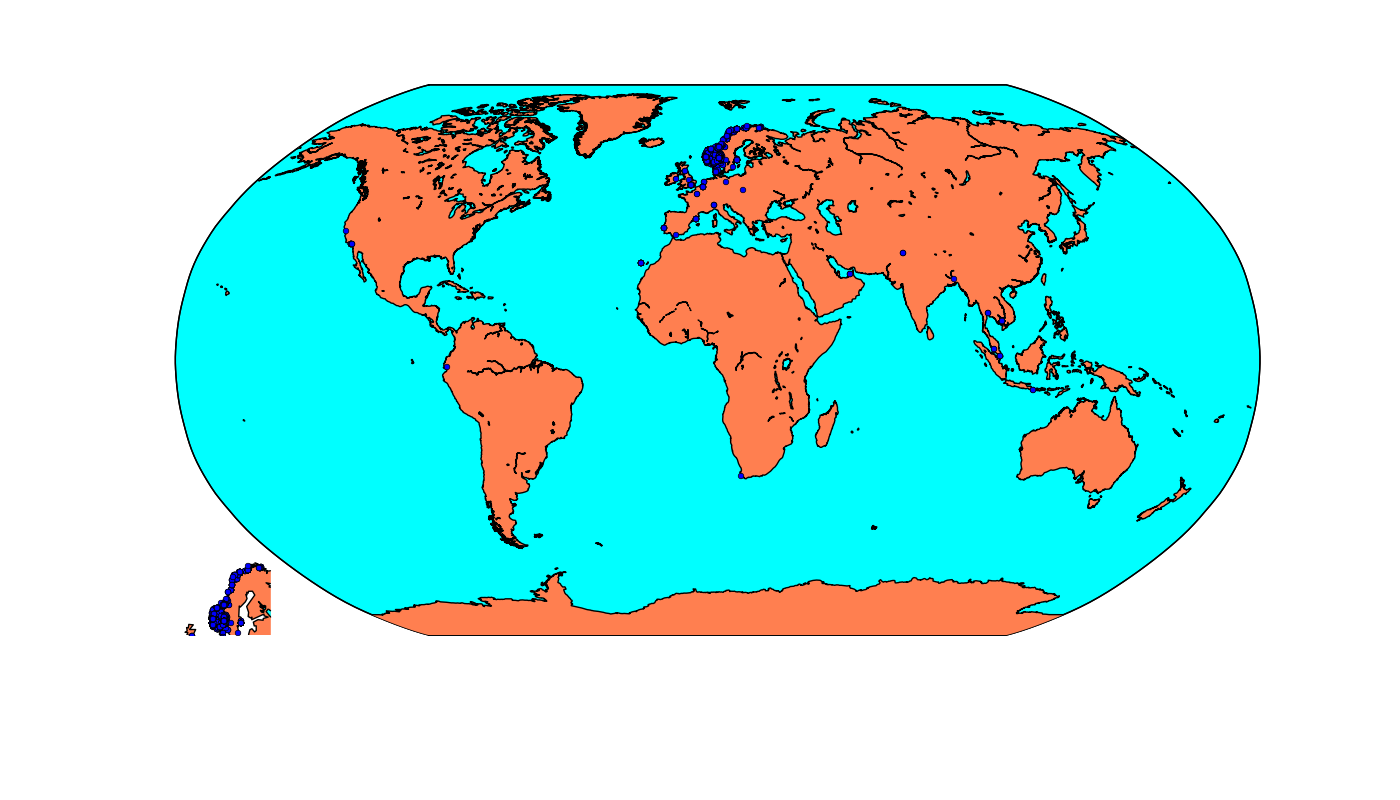
\includegraphics[width=5in]{image/simpleGeoPlotworld.png}
        \centering
        \caption[Event location mapped on the world]{This figure shows the location of the events from all over the world.
        For a cropped version with focus on Norway and the surrounding countries, refer to~\ref{figure:croppedGeoplot}}
    \end{figure}

    \begin{figure}[H]
        \includegraphics[width=5in]{image/statesInteractionFalse-gvfile.pdf}
        \centering
        \caption[States in session and how they interact]{The different states of the system and how they interact with each other.}
        \label{figure:statesInteractions}
    \end{figure}

\chapter{Extended State Of the Art}
\label{app:sota}

\section{Fashion domain}

\marginpar{TODO: Fix some kind of left align centering og content}
\begin{table}[H]
    \centering
    \begin{tabular}{ccc}
    \toprule
      \multicolumn{2}{c}{Concrete Attributes (Product Features)} & Abstract Attributes (Attitude-Based) \\
      \cmidrule(r{1em}){1-2}
      \multicolumn{1}{c}{Intrinsic (Hedonic)} & \multicolumn{1}{c}{Extrinsic} 				 	& \\ \midrule
      Style 				& Price						 	& Fun \\
      Color				& Brand 					 	& Entertainment \\
      Patten 				& Country of origin			 	& Enjoyment\\
      Fabric/fiber 		& Place(Store) 				 	& Need \\
      Appearance	   	 	& Salespeson's evaluation	 	&  Function\\
      Fashionability  	& Approval of others 		 	&\\
      Durability			& Coordination with wardrobe 	&\\
      Comfort				&								& \\
      Quality				&								& \\
      Fit					&								& \\
      Care 				&								& \\
    \bottomrule
    \end{tabular}
    \caption[Consumers' Purchase Decisions]{The attributes effecting the consumer when in the process of consuming products~\cite{dutton2006}}
    \label{table:ConsumersPurchaseDec}
\end{table}

\section{SoBazaar Competitors}\label{app:sec:soCompetitors}
\subsubsection{Flink} % (fold)
\label{par:flink}
    "Flink is THE brand-new app to discover, get inspired and share trendy looks from top fashion bloggers" - About Flink~\cite{flink}.

    Flink is a fashion discovery application for iPhone.
    It allows the user to browse fashion blogs, hot brands and new trends.

    The content displayed can be "liked" and can be a collection of clothes from different brands.
    If the user is interested in the item, the application can redirect the user to the web page where it is sold.
    \begin{table}[H]
            \centering
            \begin{tabularx}{\linewidth}{>{\parskip1ex}X@{\kern4\tabcolsep}>{\parskip1ex}X}
                \toprule
                \hfil\bfseries Strengths
                &
                \hfil\bfseries Weaknesses
                \\\cmidrule(r{3\tabcolsep}){1-1}\cmidrule(l{-\tabcolsep}){2-2}
                Can follow other users \par
                Connect with facebook \par
                Ability to add item to a \emph{want list} \par
                &
                No personalized recommendations \par
                \\\bottomrule
                \end{tabularx}
        \caption[Recommendation related strengths and weaknesses of Flink~\cite{flink}]{This table is the list of the recommendation related strengths and weaknesses of the mobile fashion application Flink~\cite{flink}}
        \label{table:iphoneAppFlink}
    \end{table}
  % todo - might be more, but can't explore the application since it is iOS 7 required
% paragraph flink (end)

\subsubsection{Motilo} % (fold)
\label{par:motilo}
    "Motilo was launched in 2011 to answer that perennial fashion dilemma all women face --- what shall I wear tonight?" - About Motilo~\cite{motilo}.

    Items on the web page are gathered by the Motilo stylists.
    This gives the page a fresh set of items for the user to select from.

    Motilo gives the user the ability to put together item sets through dragging and dropping the items into a "fashion dilemma", or simply like items.
    The user can ask friends, the Motilo community or the Motilo stylists about suggestions regarding what to wear.
    If the user wants to buy an item, Motilo redirects the user to the page which sells the item in question.

    \begin{table}[H]
    \centering
    \begin{tabularx}{\linewidth}{>{\parskip1ex}X@{\kern4\tabcolsep}>{\parskip1ex}X}
        \toprule
        \hfil\bfseries Strengths
        &
        \hfil\bfseries Weaknesses
            \\\cmidrule(r{3\tabcolsep}){1-1}\cmidrule(l{-\tabcolsep}){2-2}
            Connected with facebook \par
            Ability to add item to a "want list" \par
            A feed with the most trending item collections \par
            Ask Motilo stylists for suggestions \par
            &
            Manual/limited personalized recommendations \par
            \\\bottomrule
            \end{tabularx}
            \caption[Recommendation related strengths and weaknesses of Motilo~\cite{motilo}]{This table is the list of the recommendation related strengths and weaknesses of e-commerce fashion web site Motilo~\cite{motilo}}
            \label{table:ecommenreceMotilo}
        \end{table}
% paragraph motilo (end)


\subsubsection{ModCloth} % (fold)
\label{par:modcloth}
    "A top e-retailer of indie clothing, accessories, and decor, and provide an engaging shopping experience where you, our customer, can have a voice" - About ModCloth~\cite{modcloth}

    ModCloth focuses on giving what the community is looking for.
    The user is given the opportunity to both be the seller and the buyer.
    The item base is affected by the user trough voting.
    \begin{table}[H]
            \centering
            \begin{tabularx}{\linewidth}{>{\parskip1ex}X@{\kern4\tabcolsep}>{\parskip1ex}X}
                \toprule
                \hfil\bfseries Strengths
                &
                \hfil\bfseries Weaknesses
                \\\cmidrule(r{3\tabcolsep}){1-1}\cmidrule(l{-\tabcolsep}){2-2}
                Ability to add item to a "want list" \par
                A feed with the most popular items \par
                A feed with new items \par
                A list of similar items \par
                &
                No personalized recommendations \par
                \\ \bottomrule
        \end{tabularx}
        \caption[Recommendation related strengths and weaknesses of
        ModCloth~\cite{modcloth}]{This table is the list of the recommendation
        related strengths and weaknesses of e-commerce fashion web site
        ModCloth~\cite{modcloth}}
        \label{table:ecommenreceModCloth}
    \end{table}
% paragraph modcloth (end)

\subsubsection{UsTrendy} % (fold)
\label{par:ustrendy}
    "UsTrendy allows you to shop and discover one-of-a-kind fashions from all over the world." - About UsTrendy~\cite{UsTrendy}

    UsTrendy has a large item database of more than hundred thousand unique items.

    When the user is viewing an item, UsTrendy displays other items the user might like, which have common traits with the one the user is currently watching.
    The currently viewed item can be added to a sopping cart.
    \begin{table}[H]
                \centering
                \begin{tabularx}{\linewidth}{>{\parskip1ex}X@{\kern4\tabcolsep}>{\parskip1ex}X}
                    \toprule
                    \hfil\bfseries Strengths
                    &
                    \hfil\bfseries Weaknesses
                    \\\cmidrule(r{3\tabcolsep}){1-1}\cmidrule(l{-\tabcolsep}){2-2}
                  Ability to add item to a "want list" \par
                  A feed with the most popular items \par
                  A feed with new items \par
                  A list of similar items \par
                  &
                  No personalized recommendations \par
                \\ \bottomrule
        \end{tabularx}
        \caption[Recommendation related strengths and weaknesses of UsTrendy~\cite{UsTrendy}]{This table is the list of the recommendation related strengths and weaknesses of e-commerce fashion web site UsTrendy~\cite{UsTrendy}}
        \label{table:ecommenreceUsTrendy}
    \end{table}
% paragraph ustrendy (end)

\subsubsection{Polyvore} % (fold)
\label{par:polyvore}
    "Polyvore is a new way to discover and shop for things you love." - About Polyvore~\cite{polyvore}

    In Polyvore the user can put together sets of items and show them off to their friends and others.
    The items shown on Polyvore are gathered based on the community of Polyvore.

    When accessing an item the user is shown similar items to the one which is currently being watched.
    When the user want to purchase an item, the user is redirected to the page which sells the item.
    \begin{table}[H]
                \centering
                \begin{tabularx}{\linewidth}{>{\parskip1ex}X@{\kern4\tabcolsep}>{\parskip1ex}X}
                \toprule
                \hfil\bfseries Strengths
                &
                \hfil\bfseries Weaknesses
                \\\cmidrule(r{3\tabcolsep}){1-1}\cmidrule(l{-\tabcolsep}){2-2}
                    Ability to add item to a "want list" \par
                    The user can follow other users \par
                    Crawl other fashion sites to add to their item base \par
                    A feed with trending items \par
                    A list of recently viewed items \par
                &
                    No personalized recommendations \par
                \\ \bottomrule
        \end{tabularx}
        \caption[Recommendation related strengths and weaknesses of
        Polyvore~\cite{polyvore}]{This table is the list of the recommendation
        related strengths and weaknesses of e-commerce fashion web site
        Polyvore~\cite{polyvore}}
        \label{table:ecommenrecePolyvore}
    \end{table}
% paragraph polyvore (end)

\subsubsection{Clothia} % (fold)
\label{par:clothia}
    "An online destination where you can mix and match outfits, share looks you love, even try on clothes virtually via your webcam using augmented reality technology" - About Clothia~\cite{clothia}

    The user can put together a set of clothes from the web site and make a "set".
    The set can be shared with other users and like by other users.
    If the user is interested in buying an item, the user is redirected to the page from which the item is sold.
    \begin{table}[H]
                \centering
                \begin{tabularx}{\linewidth}{>{\parskip1ex}X@{\kern4\tabcolsep}>{\parskip1ex}X}
                \toprule
                \hfil\bfseries Strengths
                &
                \hfil\bfseries Weaknesses
                \\\cmidrule(r{3\tabcolsep}){1-1}\cmidrule(l{-\tabcolsep}){2-2}
                Ability to add item to a "want list" \par
                The user can follow other users \par
                A feed with trending items \par
                &
                Lack personalized recommendations \par
                \\ \bottomrule
        \end{tabularx}
        \caption[Recommendation related strengths and weaknesses of Clothia~\cite{clothia}]{This table is the list of the recommendation related strengths and weaknesses of e-commerce fashion web site Clothia~\cite{clothia}}
        \label{table:ecommenreceClothia}
    \end{table}
% paragraph clothia (end)

\subsubsection{Trendabl} % (fold)
\label{par:trendabl}
    "Trendabl is a community of people who love fashion" - About Trendable~\cite{trendabl}

    The user is shown a feed with the newest items, and is free to browse different sets of collections, such as collections with shoes and pants.
    If the user wants to buy an item it can be added to a shopping chart.
    \begin{table}[H]
                    \centering
                    \begin{tabularx}{\linewidth}{>{\parskip1ex}X@{\kern4\tabcolsep}>{\parskip1ex}X}
                    \toprule
                    \hfil\bfseries Strengths
                    &
                    \hfil\bfseries Weaknesses
                    \\\cmidrule(r{3\tabcolsep}){1-1}\cmidrule(l{-\tabcolsep}){2-2}
                    Ability to add item to a "want list" \par
                    The user can follow other users \par
                    System recommends the top users in the system for the user to follow \par
                    &
                    No personalized recommendations \par
                    \\ \bottomrule
        \end{tabularx}
        \caption[Recommendation related strengths and weaknesses of Trendabl~\cite{trendabl}]{This table is the list of the recommendation related strengths and weaknesses of e-commerce fashion web site Trendabl~\cite{trendabl}}
        \label{table:ecommenreceTrendabl}
    \end{table}
% paragraph trendabl (end)


\subsubsection{Rue La La} % (fold)
\label{par:rue_la_la}
    "Rue La La is the destination for the most desired brands" - About Rue La La~\cite{RueLaLa}

    Rue La La is a sale on site e-commerce web site.
    It is built up of a set of different boutiques, which can be browsed by the user.
    When the user is watching an item, Rue La La shows other items from the current boutique.

    \begin{table}[H]
                \centering
                \begin{tabularx}{\linewidth}{>{\parskip1ex}X@{\kern4\tabcolsep}>{\parskip1ex}X}
                \toprule
                \hfil\bfseries Strengths
                &
                \hfil\bfseries Weaknesses
                \\\cmidrule(r{3\tabcolsep}){1-1}\cmidrule(l{-\tabcolsep}){2-2}
                Ability to add item to a "want list" \par
                List of most popular items \par
                &
                No personalized recommendations \par
                \\ \bottomrule
        \end{tabularx}
        \caption[Recommendation related strengths and weaknesses of Rue La La~\cite{RueLaLa}]{This table is the list of the recommendation related strengths and weaknesses of e-commerce fashion web site Rue La La~\cite{RueLaLa}}
        \label{table:ecommenreceRueLaLa}
    \end{table}
% paragraph rue_la_la (end)

\subsubsection{Zalando} % (fold)
\label{par:zalando}
    "Clothes, accessories, sports items, beauty products" - About Zalando~\cite{Zalando}

    Zalando has a large set of items.
    When browsing an item the user is shown a set of similar items the user might also like, and a set of items which might "go well"  with the currently viewed item.

    \begin{table}[H]
                    \centering
                    \begin{tabularx}{\linewidth}{>{\parskip1ex}X@{\kern4\tabcolsep}>{\parskip1ex}X}
                    \toprule
                    \hfil\bfseries Strengths
                    &
                    \hfil\bfseries Weaknesses
                    \\\cmidrule(r{3\tabcolsep}){1-1}\cmidrule(l{-\tabcolsep}){2-2}
                    Ability to add item to a "want list" \par
                    Shop on site \par
                    Similar items \par
                    &
                    No personalized recommendations \par
                    \\ \bottomrule
        \end{tabularx}
        \caption[Recommendation related strengths and weaknesses of Zalando~\cite{Zalando}]{This table is the list of the recommendation related strengths and weaknesses of e-commerce fashion web site Zalando~\cite{Zalando}}
        \label{table:ecommenreceZalando}
    \end{table}
% paragraph zalando (end)

\subsubsection{Ellos~\cite{Ellos}} % (fold)
\label{par:ellos}
    Ellos is a e-commerce web site, which specializes in fashion.

    When browsing an item, similar items to the one currently being watched is presented to the user.
    Other items which might go well with the item is also presented for the user.

    \begin{table}[H]
                \centering
                \begin{tabularx}{\linewidth}{>{\parskip1ex}X@{\kern4\tabcolsep}>{\parskip1ex}X}
                \toprule
                \hfil\bfseries Strengths
                &
                \hfil\bfseries Weaknesses
                \\\cmidrule(r{3\tabcolsep}){1-1}\cmidrule(l{-\tabcolsep}){2-2}
                Ability to add item to a "want list" \par
                Shop on site \par
                Similar items \par
                On site most popular list \par
                Items which might go well with the current \par
                &
                No personalized recommendations \par
                \\ \bottomrule
        \end{tabularx}
        \caption[Recommendation related strengths and weaknesses of Ellos~\cite{Ellos}]{This table is the list of the recommendation related strengths and weaknesses of e-commerce fashion web site Ellos~\cite{Ellos}}
        \label{table:ecommenreceEllos}
    \end{table}
% paragraph ellos (end)

\subsubsection{LookBook} % (fold)
\label{par:lookbook}
    "LOOKBOOK is the \#1 source for fashion inspiration from real people around the world." - About LookBook~\cite{LookBook}

    LookBook is a leading online community which is centered around the looks of the users.
    The users can share their own looks and keep up with other users through watching their uploads.
    With over 1.2 million members LookBook is constantly up to date on the newest fashion trends.
    \begin{table}[H]
                \centering
                \begin{tabularx}{\linewidth}{>{\parskip1ex}X@{\kern4\tabcolsep}>{\parskip1ex}X}
                \toprule
                \hfil\bfseries Strengths
                &
                \hfil\bfseries Weaknesses
                \\\cmidrule(r{3\tabcolsep}){1-1}\cmidrule(l{-\tabcolsep}){2-2}
                Ability to add item to a "want list" \par
                Shop on site \par
                Similar items \par
                Most popular items list \par
                Hot items list \par
                &
                No personalized recommendations \par
                \\ \bottomrule
        \end{tabularx}
        \caption[Recommendation related strengths and weaknesses of LookBook~\cite{LookBook}]{This table is the list of the recommendation related strengths and weaknesses of e-commerce fashion web site LookBook~\cite{LookBook}}
        \label{table:ecommenreceLookBook}
    \end{table}
% paragraph lookbook (end)


\subsubsection{Fashiolista} % (fold)
\label{par:fashiolista}
    "Let Fashiolista's community be your style guide in the online fashion jungle" - About Fasho~\cite{Fashiolista}

    The items on Fashiolista is selected by the users of Fashiolista, and the sites is therefore customized to fit the user crowd's wishes and interests.

    When accessing an item, the user is presented with the item, and a set of other items from the store the current item originated from.
    Other users who liked the item are also shown, so the user can browse their personal want list.
    \begin{table}[H]
                    \centering
                    \begin{tabularx}{\linewidth}{>{\parskip1ex}X@{\kern4\tabcolsep}>{\parskip1ex}X}
                    \toprule
                    \hfil\bfseries Strengths
                    &
                    \hfil\bfseries Weaknesses
                    \\\cmidrule(r{3\tabcolsep}){1-1}\cmidrule(l{-\tabcolsep}){2-2}
                Ability to add item to a "want list" \par
                On site most popular list \par
             &
                 No personalized recommendations \par
             \\ \bottomrule
        \end{tabularx}
        \caption[Recommendation related strengths and weaknesses of Fashiolista~\cite{Fashiolista}]{This table is the list of the recommendation related strengths and weaknesses of e-commerce fashion web site Fashiolista~\cite{Fashiolista}}
        \label{table:ecommenreceFahiolista}
    \end{table}
% paragraph fashiolista (end)

\subsubsection{ShopStyle} % (fold)
\label{par:shopstyle}
    "POPSUGAR is a global women's lifestyle brand focused in media, commerce, and technology" - About ShopStyle~\cite{ShopStyle}

    ShopStyle is a commerce brand of POPSUGAR.
    ShopStyle displays items from other e-commerce web sites, and redirects the user directly to the e-commerce web site from which the item clicked originated.
    Items can be liked on ShopStyle, and viewed in less detail at the web page of ShopStyle.
    \begin{table}[H]
                    \centering
                    \begin{tabularx}{\linewidth}{>{\parskip1ex}X@{\kern4\tabcolsep}>{\parskip1ex}X}
                    \toprule
                    \hfil\bfseries Strengths
                    &
                    \hfil\bfseries Weaknesses
                    \\\cmidrule(r{3\tabcolsep}){1-1}\cmidrule(l{-\tabcolsep}){2-2}
                Ability to add item to a "want list" \par
                Similar items \par
                Editor's picks \par
            &
                No personalized recommendations \par
            \\ \bottomrule
        \end{tabularx}
        \caption[Recommendation related strengths and weaknesses of ShopStyle~\cite{ShopStyle}]{This table is the list of the recommendation related strengths and weaknesses of e-commerce fashion web site ShopStyle~\cite{ShopStyle}}
        \label{table:ecommenreceShopStyle}
    \end{table}
% paragraph shopstyle (end)

\section{State of the Art: Evaluation}
\label{appendix:evaluation-metrics}

% Describe why this is in the Appendix.
In this section we will cover an in-depth study of evaluation metrics and
methods, which were not included in~\ref{sec:evaluation} as they are not
directly suited for either the domain or setting in the proposed system.
They are included here as they may provide clarity on \textit{why} they are not
suited, as well the fact that non-suitednes is a result in itself. Finally we
identify some resources of which the avid reader may do further research into
the field of evaluation recommender systems.

% Boostrapping in Appendix, as we do not use it and Helge proposed it.
\subsubsection{Using bootstrapping for validating offline experiments}
Bootstrapping~\cite{efron1994introduction} is used to estimate properties of an
estimate, such as bias, variance, confidence, intervals and prediction error.
This is done trough measuring these properties when sampling from an
approximated distribution, creating an empirical distribution of the observed
data.  Since the entire population is unknown it will not be possible to
calculate the true error from the sample data.  The idea then is that with this
information from sample data it is possible to say something about the
population.  Since it will not be possible to perform inference on:

\emph{sample data} $\rightarrow$ \emph{population} this is modeled as:
\emph{re-sample data} $\rightarrow$ \emph{sample data}.
The \emph{re-sample data} is a re-sampling of the sample data.

In practice an example to bootstrapping is when we want to calculate the
average height of the population worldwide.  The issue here is that it is not
as doable to measure everyone, so a subset of the population is used.  Since
the average on this number only will be an estimate of the actual world wide
average a sense of error margin must be introduced.  Bootstrapping is then used
to reduce the error of margin through re-sampling the sample data a large
number of times~\footnote{Numbers vary on sample size, but is often 1 000 to 10
000}, and new averages are calculated.  With these averages a histogram can be
produced, which provides an estimate of the distribution of this average.

\begin{figure}[H]
    \includegraphics[scale=0.6]{image/bootstrap.png}
    \centering
    \caption[Bootstrapping principles]{A figure of the principles bootstrapping. Taken from~\cite{Eichler2003}}
    \label{figure:bootstrapping}
\end{figure}

One prominent issue with bootstrapping is that important properties of the
actual data might not be caught when undertaking the bootstrapping analysis
~\footnote{"Bootstrapping" comes from the phrase, "to pull oneself up by one's
bootstraps"~\cite{bootstrapSaying1843}}.

% Sub-section on resources available for avid readers who want further research
% into the field of evaluating recommender systems.
\subsubsection{Datasets for Offline Evaluation}
The main aim of a recommender system is to identify the set of items in a
dataset that might be interesting to a user based on their expressed
preferences. For a fashion recommender this would mean estimating how much a
user might like an item, by e.g.\\ predicting what rating a user might give an
item. In recent years, various test collections for different domains such as
books, music, movies have been made available to the public. These datasets
usually consist of user ratings similar to the ones used in this thesis (see
Section~\ref{}):

\begin{table}[H]
\centering
	\begin{tabular}{*{4}l}
	\toprule
		User ID & Item ID & Rating & Timestamp \\ \midrule
		1		  &	11	  &	5	    &  2014-12-15 10:14:51  \\
		2		  &	19	  &	2	    &  2014-12-12 11:44:31  \\
		\dots &	\dots &	\dots &  \dots                \\
	\bottomrule
	\end{tabular}
\caption{Classical recommender system dataset}
\end{table}

In recent years more or more datasets have been made available which contains
additional information such as demographic information about the users,
trust-networks, user-assigned tags and etc. Below we have listed a few selected
popular datasets containing additional information:

\begin{itemize}

\item \textbf{MovieLens 100k dataset}~\cite{Movielens}: The movielens dataset
	incorporates demographic information about the user in addition the
	traditional rating matrix

\item \textbf{Epinions dataset}~\cite{Epinions}: The Epinions dataset includes a
	trust-network, which specifices who-trust-whom in a social network based on
	customer reviews for the website Epinions.com

\item \textbf{The Million Song Dataset}~\cite{Bertin-Mahieux2011}: The million song
	dataset is a implicit feedback dataset. This data also includes information on the users,
	and audio features and song meta-data.

\item \textbf{The Book-Crossing Dataset}: The bookcrossing dataset consists of both implicit and explicit feedback,
	demographic information about users and some content based information about the books.
\end{itemize}

\chapter{Extended Implementation}
\label{app:impl}

\section{Implemented Functional Requirements}
\begin{enumerate}[label=\bfseries FR \arabic*:]
  \item {\color{ForestGreen}Blablaba}
  \item {\color{RedOrange}\st{Blablaba}}
\end{enumerate}

\section{Implemented Non Functional Requirements}
\begin{enumerate}[label=\bfseries NFR \arabic*:]
  \item {\color{ForestGreen}Blablaba}
  \item {\color{RedOrange}\st{Blablaba}}
\end{enumerate}

\section{Experimental Results}
\label{app:results}


%----------------------------------------------
% BIBLIOGRAPHY
%----------------------------------------------
\clearpage
\addcontentsline{toc}{chapter}{References}
\bibliographystyle{plain}
\bibliography{references}

\end{document}
